\PassOptionsToPackage{obeyspaces}{url}
\documentclass[cn,11pt]{elegantbook}

\usepackage[labelformat=simple,listofformat=subsimple]{subfig}
\usepackage{longtable}
\usepackage[boxed]{algorithm2e}
\usepackage{makecell}
\usepackage{rotating}
\usepackage{wrapfig}
\usepackage{tikz}
\usepackage{forest}
\usepackage{pgfplots}
\usepackage{multirow}
\usepackage{verbatim}

\pgfplotsset{compat=1.6}
\hypersetup{bookmarksdepth=5}
\lstset{language={C++}}

\AtBeginDocument{
	\setcounter{tocdepth}{0}
}

\renewcommand{\figureautorefname}{图}
\renewcommand{\tableautorefname}{表}
\renewcommand{\sectionautorefname}{节}
\renewcommand{\subsectionautorefname}{小节}
\renewcommand{\chapterautorefname}{章}
\renewcommand{\algorithmautorefname}{算法}
\renewcommand{\algorithmcfname}{算法}
\newcommand{\examautorefname}{例}
\newcommand{\probautorefname}{例题}
\renewcommand\thesubfigure{(\alph{subfigure})}
\newcommand{\subfigureautorefname}{\figureautorefname}
\renewcommand\thesubtable{(\alph{subtable})}
\newcommand{\subtableautorefname}{\tableautorefname}
\newcommand{\wiki}[1]{\href{https://terraria.wiki.gg/zh/wiki/#1}{#1}}
\newcommand{\wikii}[2]{\href{https://terraria.wiki.gg/zh/wiki/#1}{#2}}
\setcounter{totalnumber}{100}
\makeatletter
\g@addto@macro\UrlBreaks{%
 \do\.\do\@\do\\\do\/\do\!\do\_\do\|\do\;\do\>\do\]%这里没有语法问题,属于分析器bug
 \do\)\do\,\do\?\do\&\do\'\do+\do\=\do\#}
\makeatother

\newcommand{\DMC}{死人的宝箱}
\newcommand{\FM}{Fog Machine}
\newcommand{\Grate}{格栅}
\newcommand{\PL}{Plasma Lamp}
\newcommand{\Volcano}{Volcano}
\newcommand{\GC}{高尔夫球洞}
\newcommand{\Lesion}{损伤}
\newcommand{\Bamboo}{竹}

\usepackage{xstring}

\newcommand{\titem}[1]{
  \IfEqCase{#1}{
    {148}{水蜡烛}
  }
}

\newcommand{\tnpc}[1]{
  \IfEqCase{#1}{
    {4}{克苏鲁之眼}
    {26}{哥布林苦力}
    {27}{哥布林盗贼}
    {28}{哥布林战士}
    {29}{哥布林巫士}
    {35}{骷髅王头部}
    {46}{兔兔}
    {48}{鸟妖}
    {50}{史莱姆王}
    {55}{金鱼}
    {111}{哥布林弓箭手}
    {113}{血肉墙}
    {125}{激光眼}
    {126}{魔焰眼}
    {127}{机械骷髅王}
    {134}{毁灭者头部}
    {143}{雪人暴徒}
    {144}{戳刺先生}
    {145}{巴拉雪人}
    {163}{黑隐士}
    {164}{爬墙蜘蛛}
    {212}{海盗水手}
    {213}{私船海盗}
    {214}{海盗神射手}
    {215}{海盗弩手}
    {216}{海盗船长}
    {222}{蜂王}
    {245}{石巨人身体}
    {252}{鹦鹉}
    {262}{世纪之花}
    {266}{克苏鲁之脑}
    {299}{松鼠}
    {300}{老鼠}
    {303}{史莱姆兔兔}
    {337}{圣诞兔兔}
    {354}{织网发型师}
    {357}{蠕虫}
    {359}{蜗牛}
    {370}{猪龙鱼公爵}
    {381}{扰脑怪}
    {382}{激光枪手}
    {383}{火星军官}
    {385}{灰咕噜兽}
    {386}{火星工程师}
    {388}{火星飞船}
    {389}{电击怪}
    {390}{鳞甲怪枪手}
    {395}{火星飞碟核心}
    {396}{月亮领主头部}
    {397}{月亮领主手}
    {398}{月亮领主心脏}
    {399}{火星探测器}
    {402}{银河织妖头部}
    {405}{星细胞}
    {407}{流体入侵怪}
    {409}{闪耀炮手}
    {411}{观星怪}
    {412}{千足蜈蚣头部}
    {415}{火龙怪}
    {416}{火龙怪骑士}
    {417}{火滚怪}
    {418}{流星火怪}
    {419}{火月怪}
    {420}{星云浮怪}
    {421}{吮脑怪}
    {422}{星旋柱}
    {423}{进化兽}
    {424}{预言帝}
    {425}{漩泥怪}
    {426}{异星蜂王}
    {427}{异星黄蜂}
    {429}{星旋怪}
    {439}{拜月教邪教徒}
    {443}{金兔}
    {447}{金老鼠}
    {448}{金蠕虫}
    {471}{哥布林召唤师}
    {491}{荷兰飞盗船}
    {493}{星尘柱}
    {507}{星云柱}
    {517}{日耀柱}
    {518}{火龙战士}
    {520}{火星走妖}
    {538}{红松鼠}
    {539}{金松鼠}
    {540}{派对兔兔}
    {549}{神秘传送门}
    {579}{昏睡男子}
    {624}{侏儒}
    {636}{光之女皇}
    {657}{史莱姆皇后}
  }
}

\newcommand{\twall}[1]{
  \IfEqCase{#1}{
    {0}{无背景墙}
    {1}{石墙}
    {4}{木墙}
    {5}{灰砖墙}
    {6}{红砖墙}
    {10}{金砖墙}
    {11}{银砖墙}
    {12}{铜砖墙}
    {16}{人造土墙}
    {17}{人造蓝砖墙}
    {18}{人造绿砖墙}
    {19}{人造粉砖墙}
    {20}{人造黑曜石砖墙}
    {21}{玻璃墙}
    {22}{珍珠石砖墙}
    {23}{荧光砖墙}
    {24}{泥石砖墙}
    {25}{钴砖墙}
    {26}{秘银砖墙}
    {27}{板条墙}
    {29}{糖棒墙}
    {30}{绿糖棒墙}
    {31}{雪砖墙}
    {32}{精金梁墙}
    {33}{魔矿砖墙}
    {34}{沙岩砖墙}
    {35}{黑檀石砖墙}
    {36}{红泥灰墙}
    {37}{黄泥灰墙}
    {38}{绿泥灰墙}
    {39}{灰泥灰墙}
    {41}{乌木墙}
    {42}{红木墙}
    {43}{珍珠木墙}
    {44}{彩虹砖墙}
    {45}{锡砖墙}
    {46}{钨砖墙}
    {47}{铂金砖墙}
    {48}{天然紫晶墙}
    {49}{天然黄玉墙}
    {50}{天然蓝玉墙}
    {51}{天然翡翠墙}
    {52}{天然红玉墙}
    {53}{天然钻石墙}
    {60}{天然生命树叶墙}
    {62}{天然蜘蛛墙}
    {66}{人造草墙}
    {67}{人造丛林墙}
    {68}{人造花墙}
    {72}{仙人掌墙}
    {73}{云墙}
    {74}{人造蘑菇墙}
    {75}{骨块墙}
    {76}{史莱姆块墙}
    {77}{血肉块墙}
    {78}{人造生命木墙}
    {82}{飞盘墙}
    {84}{冰雪砖墙}
    {85}{暗影木墙}
    {86}{天然蜂巢墙}
    {87}{天然丛林蜥蜴砖墙}
    {88}{紫花窗玻璃}
    {89}{黄花窗玻璃}
    {90}{蓝花窗玻璃}
    {91}{绿花窗玻璃}
    {92}{红花窗玻璃}
    {93}{五彩花窗玻璃}
    {100}{人造蓝板墙}
    {101}{人造蓝瓷砖墙}
    {102}{人造粉板墙}
    {103}{人造粉瓷砖墙}
    {104}{人造绿板墙}
    {105}{人造绿瓷砖墙}
    {106}{木栅栏}
    {107}{铅栅栏}
    {108}{人造蜂巢墙}
    {109}{钯金柱墙}
    {110}{泡泡糖块墙}
    {111}{钛石块墙}
    {112}{人造丛林蜥蜴砖墙}
    {113}{南瓜墙}
    {114}{干草墙}
    {115}{阴森木墙}
    {116}{圣诞树壁纸}
    {117}{装饰壁纸}
    {118}{糖棒壁纸}
    {119}{节日壁纸}
    {120}{星星壁纸}
    {121}{波浪条纹壁纸}
    {122}{雪花壁纸}
    {123}{坎卜斯犄角壁纸}
    {124}{蓝绿壁纸}
    {125}{格林奇手指壁纸}
    {126}{别致灰壁纸}
    {127}{浮冰壁纸}
    {128}{音符壁纸}
    {129}{紫雨壁纸}
    {130}{彩虹壁纸}
    {131}{烁石壁纸}
    {132}{星光天堂壁纸}
    {133}{泡泡壁纸}
    {134}{铜管壁纸}
    {135}{黄鸭壁纸}
    {136}{瀑布墙}
    {137}{熔岩瀑布墙}
    {138}{乌木栅栏}
    {139}{红木栅栏}
    {140}{珍珠木栅栏}
    {141}{暗影木栅栏}
    {142}{白王朝墙}
    {143}{蓝王朝墙}
    {144}{奥术神符墙}
    {145}{铁栅栏}
    {146}{镀铜墙}
    {147}{石板墙}
    {148}{船帆}
    {149}{针叶木墙}
    {150}{针叶木栅栏}
    {151}{棕榈木墙}
    {152}{棕榈木栅栏}
    {153}{琥珀晶莹宝石墙}
    {154}{紫晶晶莹宝石墙}
    {155}{钻石晶莹宝石墙}
    {156}{翡翠晶莹宝石墙}
    {157}{黯淡琥珀晶莹宝石墙}
    {158}{黯淡紫晶晶莹宝石墙}
    {159}{黯淡钻石晶莹宝石墙}
    {160}{黯淡翡翠晶莹宝石墙}
    {161}{黯淡红玉晶莹宝石墙}
    {162}{黯淡蓝玉晶莹宝石墙}
    {163}{黯淡黄玉晶莹宝石墙}
    {164}{红玉晶莹宝石墙}
    {165}{蓝玉晶莹宝石墙}
    {166}{黄玉晶莹宝石墙}
    {167}{镀锡墙}
    {168}{彩纸墙}
    {169}{午夜彩纸墙}
    {172}{蜂蜜瀑布墙}
    {173}{叶绿砖墙}
    {174}{猩红矿砖墙}
    {175}{蘑菇矿镀层墙}
    {176}{火星管道墙}
    {177}{人造狱石砖墙}
    {178}{天然大理石墙}
    {179}{光面大理石墙}
    {180}{天然花岗岩墙}
    {181}{光面花岗岩墙}
    {182}{陨石砖墙}
    {183}{人造大理石墙}
    {184}{人造花岗岩墙}
    {186}{水晶块墙}
    {187}{天然沙岩墙}
    {216}{天然硬化沙墙}
    {217}{天然硬化黑檀沙墙}
    {218}{天然硬化猩红沙墙}
    {219}{天然硬化珍珠沙墙}
    {220}{天然黑檀沙岩墙}
    {221}{天然猩红沙岩墙}
    {222}{天然珍珠沙岩墙}
    {223}{天然沙漠化石墙}
    {224}{夜明砖墙}
    {225}{齿轮墙}
    {226}{沙暴墙}
    {227}{降雪墙}
    {228}{呆萌粉气球墙}
    {229}{呆萌紫气球墙}
    {230}{呆萌绿气球墙}
    {231}{铁砖墙}
    {232}{铅砖墙}
    {233}{Lesion Block Wall}
    {234}{Crimstone Brick Wall}
    {235}{Smooth Sandstone Wall}
    {236}{Spider Nest Wall}
    {237}{Solar Brick Wall}
    {238}{Vortex Brick Wall}
    {239}{Nebula Brick Wall}
    {240}{Stardust Brick Wall}
    {241}{Orange Stained Glass}
    {242}{Gold Starry Wall}
    {243}{Blue Starry Wall}
    {244}{天然生命木墙}
    {245}{Wrought Iron Fence}
    {246}{人造黑檀石墙}
    {247}{人造泥墙}
    {248}{人造珍珠石墙}
    {249}{人造雪墙}
    {250}{人造紫晶石墙}
    {251}{人造黄玉石墙}
    {252}{人造蓝玉石墙}
    {253}{人造翡翠石墙}
    {254}{人造红玉石墙}
    {255}{人造钻石石墙}
    {256}{人造Green Mossy Wall}
    {257}{人造Brown Mossy Wall}
    {258}{人造Red Mossy Wall}
    {259}{人造Blue Mossy Wall}
    {260}{人造Purple Mossy Wall}
    {261}{人造Rocky Dirt Wall}
    {262}{人造Old Stone Wall}
    {263}{人造蜘蛛墙}
    {264}{人造腐化草墙}
    {265}{人造神圣草墙}
    {266}{人造冰墙}
    {267}{人造Obsidian Wall}
    {268}{人造猩红草墙}
    {269}{人造猩红石墙}
    {270}{人造山洞土墙}
    {271}{人造Rough Dirt Wall}
    {272}{人造大理石墙(未使用)}
    {273}{人造花岗岩墙(未使用)}
    {274}{人造Craggy Stone Wall}
    {275}{人造沙岩墙}
    {276}{人造Corrupt Growth Wall}
    {277}{人造Corrupt Mass Wall}
    {278}{人造Corrupt Pustule Wall}
    {279}{人造Corrupt Tendril Wall}
    {280}{人造Crimson Crust Wall}
    {281}{人造Crimson Scab Wall}
    {282}{人造Crimson Teeth Wall}
    {283}{人造Crimson Blister Wall}
    {284}{人造Layered Dirt Wall}
    {285}{人造Crumbling Dirt Wall}
    {286}{人造Cracked Dirt Wall}
    {287}{人造Wavy Dirt Wall}
    {288}{人造Hallowed Prism Wall}
    {289}{人造神圣洞穴墙}
    {290}{人造神圣碎块墙}
    {291}{人造Hallowed Crystalline Wall}
    {292}{人造Lichen Stone Wall}
    {293}{人造Leafy Jungle Wall}
    {294}{人造Ivy Stone Wall}
    {295}{人造Jungle Vine Wall}
    {296}{人造Ember Wall}
    {297}{人造Cinder Wall}
    {298}{人造岩浆墙}
    {299}{人造Smouldering Stone Wall}
    {300}{人造Worn Stone Wall}
    {301}{人造Stalactite Stone Wall}
    {302}{人造Mottled Stone Wall}
    {303}{人造Fractured Stone Wall}
    {304}{人造硬化沙墙}
    {305}{人造硬化黑檀沙墙}
    {306}{人造硬化猩红沙墙}
    {307}{人造硬化珍珠沙墙}
    {308}{人造黑檀沙岩墙}
    {309}{人造猩红沙岩墙}
    {310}{人造珍珠沙岩墙}
    {311}{人造沙漠化石墙}
    {312}{竹墙}
    {313}{Large Bamboo Wall}
    {314}{人造琥珀石墙}
    {315}{Bamboo Fence}
  }
}

\newcommand{\ttile}[1]{
  \IfEqCase{#1}{
    {0}{土块}
    {1}{石块}
    {2}{草}
    {3}{矮小草类植物}
    {4}{火把}
    {5}{树}
    {6}{铁矿}
    {7}{铜矿}
    {8}{金矿}
    {9}{银矿}
    {10}{门(关上)}
    {11}{门(打开)}
    {14}{桌}
    {16}{铁/铅砧}
    {18}{工作台}
    {19}{平台}
    {22}{魔矿}
    {23}{腐化草}
    {24}{腐化植物}
    {25}{黑檀石块}
    {30}{木材}
    {32}{腐化多刺灌木}
    {37}{陨石}
    {38}{灰砖}
    {39}{红砖}
    {40}{粘土块}
    {41}{蓝砖}
    {43}{绿砖}
    {44}{粉砖}
    {45}{金砖}
    {46}{银砖}
    {47}{铜砖}
    {48}{尖刺}
    {49}{水蜡烛}
    {53}{沙块}
    {54}{玻璃}
    {56}{黑曜石}
    {57}{灰烬块}
    {58}{狱石}
    {59}{泥块}
    {60}{丛林草}
    {61}{矮小丛林植物}
    {62}{丛林蔓藤}
    {63}{蓝玉块}
    {64}{红玉块}
    {65}{翡翠块}
    {66}{黄玉块}
    {67}{紫晶块}
    {68}{钻石块}
    {70}{蘑菇草}
    {71}{生长的发光蘑菇}
    {72}{地下巨型发光蘑菇}
    {74}{高大丛林植物}
    {75}{黑曜石砖}
    {76}{狱石砖}
    {85}{墓石}
    {87}{钢琴}
    {88}{梳妆台}
    {101}{书架}
    {107}{钴矿}
    {108}{秘银矿}
    {109}{神圣草}
    {110}{矮小神圣植物}
    {111}{精金矿}
    {112}{黑檀沙块}
    {113}{高大神圣植物}
    {114}{工匠作坊}
    {116}{珍珠沙块}
    {117}{珍珠石块}
    {118}{珍珠石砖}
    {119}{荧光砖}
    {120}{泥石砖}
    {121}{钴砖}
    {122}{秘银砖}
    {123}{泥沙块}
    {127}{冰块(冰雪魔杖)}
    {130}{通电石块}
    {134}{秘银/山铜砧}
    {137}{机关}
    {138}{巨石}
    {140}{魔矿砖}
    {145}{糖棒块}
    {146}{绿糖棒块}
    {147}{雪块}
    {148}{雪砖}
    {150}{精金梁}
    {151}{沙岩砖}
    {152}{黑檀石砖}
    {153}{红泥灰}
    {154}{黄泥灰}
    {155}{绿泥灰}
    {156}{灰泥灰}
    {157}{乌木}
    {158}{红木}
    {159}{珍珠木}
    {160}{彩虹砖}
    {161}{冰雪块}
    {162}{薄冰}
    {163}{紫冰雪块}
    {164}{粉冰雪块}
    {166}{锡矿}
    {167}{铅矿}
    {168}{钨矿}
    {169}{铂金矿}
    {170}{松树块}
    {175}{锡砖}
    {176}{钨砖}
    {177}{铂金砖}
    {179}{青绿苔藓}
    {180}{黄绿苔藓}
    {181}{红苔鲜}
    {182}{蓝苔藓}
    {183}{紫苔藓}
    {188}{仙人掌(放置)}
    {189}{云}
    {190}{发光蘑菇(放置)}
    {191}{生命木}
    {192}{树叶块}
    {193}{史莱姆块}
    {194}{骨块}
    {195}{血肉块}
    {196}{雨云}
    {197}{冰冻史莱姆块}
    {198}{沥青块}
    {199}{猩红草}
    {200}{红冰雪块}
    {202}{日盘块}
    {203}{猩红石块}
    {204}{猩红矿}
    {206}{冰雪砖}
    {208}{暗影木}
    {211}{叶绿矿}
    {221}{钯金矿}
    {222}{山铜矿}
    {223}{钛金矿}
    {224}{雪泥块}
    {225}{蜂巢}
    {226}{丛林蜥蜴砖}
    {229}{蜂蜜块}
    {230}{松脆蜂蜜块}
    {232}{木尖刺}
    {234}{猩红沙块}
    {235}{传送机}
    {239}{锭}
    {248}{钯金柱}
    {249}{泡泡糖块}
    {250}{钛石块}
    {251}{南瓜}
    {252}{干草}
    {253}{阴森木}
    {255}{紫晶晶莹宝石块(黯淡)}
    {256}{黄玉晶莹宝石块(黯淡)}
    {257}{蓝玉晶莹宝石块(黯淡)}
    {258}{翡翠晶莹宝石块(黯淡)}
    {259}{红玉晶莹宝石块(黯淡)}
    {260}{钻石晶莹宝石块(黯淡)}
    {261}{琥珀晶莹宝石块(黯淡)}
    {262}{紫晶晶莹宝石块(激活)}
    {263}{黄玉晶莹宝石块(激活)}
    {264}{蓝玉晶莹宝石块(激活)}
    {265}{翡翠晶莹宝石块(激活)}
    {266}{红玉晶莹宝石块(激活)}
    {267}{钻石晶莹宝石块(激活)}
    {268}{琥珀晶莹宝石块(激活)}
    {272}{齿轮}
    {273}{石板}
    {274}{沙岩板}
    {284}{铜镀层}
    {311}{王朝木}
    {312}{红王朝瓦}
    {313}{蓝王朝瓦}
    {315}{珊瑚石块}
    {321}{针叶木}
    {322}{棕榈木}
    {325}{锡镀层}
    {326}{瀑布块}
    {327}{熔岩瀑布块}
    {328}{彩纸块}
    {329}{午夜彩纸块}
    {345}{蜂蜜瀑布块}
    {346}{叶绿砖}
    {347}{猩红矿砖}
    {348}{蘑菇矿镀层}
    {350}{火星管道镀层}
    {352}{猩红多刺灌木}
    {357}{光面大理石块}
    {367}{大理石块}
    {368}{花岗岩块}
    {369}{光面花岗岩块}
    {370}{陨石砖}
    {371}{粉史莱姆块}
    {372}{和平蜡烛}
    {376}{宝匣}
    {379}{泡泡}
    {380}{种植盆}
    {381}{火焰苔藓}
    {383}{生命红木}
    {384}{红木树叶墙}
    {385}{水晶块}
    {387}{机关门(关上)}
    {388}{高门(关上)}
    {396}{沙岩块}
    {397}{硬化沙块}
    {398}{硬化黑檀沙块}
    {399}{硬化猩红沙块}
    {400}{黑檀沙岩块}
    {401}{猩红沙岩块}
    {402}{硬化珍珠沙块}
    {403}{珍珠沙岩块}
    {404}{沙漠化石}
    {405}{壁炉}
    {407}{坚固头盔}
    {408}{夜明矿}
    {409}{夜明砖}
    {415}{日耀碎片块}
    {416}{星旋碎片块}
    {417}{星云碎片块}
    {418}{星尘碎片块}
    {421}{传送带(顺时针)}
    {422}{传送带(逆时针)}
    {426}{红团队块}
    {427}{红团队平台}
    {430}{绿团队块}
    {431}{蓝团队块}
    {432}{黄团队块}
    {433}{粉团队块}
    {434}{白团队块}
    {435}{绿团队平台}
    {436}{蓝团队平台}
    {437}{黄团队平台}
    {438}{粉团队平台}
    {439}{白团队平台}
    {446}{呆萌粉气球}
    {447}{呆萌紫气球}
    {448}{呆萌绿气球}
    {458}{沙暴块}
    {459}{降雪块}
    {460}{雪云}
    {469}{水晶桌}
    {472}{铁砖}
    {473}{铅砖}
    {474}{损伤块}
    {476}{高尔夫球洞}
    {477}{Mowed Grass}
    {478}{猩红石砖}
    {479}{Smooth Sandstone}
    {481}{Cracked Blue Brick}
    {482}{Cracked Green Brick}
    {483}{Cracked Pink Brick}
    {484}{Rolling Cactus}
    {492}{Mowed Hallowed Grass}
    {495}{Shell Pile}
    {496}{反入口块}
    {498}{蜘蛛巢块}
    {500}{日耀砖}
    {501}{星旋砖}
    {502}{星云砖}
    {503}{星尘砖}
    {507}{Gold Starry Block}
    {508}{Blue Starry Block}
    {512}{绿苔藓(灰砖)}
    {513}{黄绿苔藓(灰砖)}
    {514}{红苔鲜(灰砖)}
    {515}{蓝苔藓(灰砖)}
    {516}{紫苔藓(灰砖)}
    {517}{火焰苔藓(灰砖)}
    {528}{Mushroom Vines}
    {534}{Krypton Moss}
    {535}{Krypton Moss(灰砖)}
    {536}{Xenon Moss}
    {537}{Xenon Moss(灰砖)}
    {539}{Argon Moss}
    {540}{Argon Moss(灰砖)}
    {541}{回声块}
    {546}{格栅}
    {557}{格栅(关闭)}
    {562}{竹}
    {563}{Large Bamboo}
    {566}{Amber Stone Block}
    {618}{Stone Accent Slab}
  }
}

\newcommand{\tzone}[1]{
  \IfEqCase{#1}{
    {dungeon}{\hyperref[app37]{地牢环境}}
    {cavern}{\hyperref[app45]{洞穴层}}
    {corruption}{\hyperref[app37]{腐化环境}}
    {crimson}{\hyperref[app37]{猩红环境}}
    {graveyard}{\hyperref[app37]{墓地环境}}
    {meteor}{\hyperref[app37]{陨石环境}}
    {oldonearmy}{\hyperref[app46]{撒旦军团环境}}
    {pillar}{\hyperref[app46]{天界柱环境}}
    {space}{\hyperref[app45]{太空层}}
    {surface}{\hyperref[app45]{地表层}}
    {underground}{\hyperref[app45]{地下层}}
    {underworld}{\hyperref[app45]{地狱层}}
    {watercandle}{\hyperref[app37]{水蜡烛环境}}
  }
}

\newcommand{\tset}[1]{
  \IfEqCase{#1}{
    {boss}{\hyperref[app49]{Boss}}
    {DangerThatPreventsOtherDangers}{\hyperref[app49]{独立危险源}}
    {HardenedSand}{\hyperref[app9]{转化硬化沙墙}}
    {IsSkippedForNPCSpawningGroundTypeCheck}{\hyperref[app48]{传送带}}
    {Sandstone}{\hyperref[app9]{转化沙岩墙}}
    {tileDungeon}{\hyperref[app48]{地牢砖}}
    {tileSolid}{\hyperref[app47]{实体块}}
    {tileSolidTop}{\hyperref[app48]{平台类}}
    {wallHouse}{\hyperref[app39]{人工背景墙}}
    {wallLight}{\hyperref[app9]{透光墙}}
  }
}

\newcommand{\tcheck}[2]{
  \IfEqCase{#1}{
    {AnyDanger}{\IfEqCase{#2}{{true}{世界中存在\nameref{app41}}{false}{世界中不存在\nameref{app41}}}}
    {FlyingAntlionCheck}{\IfEqCase{#2}{{true}{通过了\nameref{app53}}{false}{未通过\nameref{app53}}}}
  }
}


\title{Terraria 电路文档}
\subtitle{最全面的Terraria电路参考资料}

% 这部分不要删掉任何一个属性,否则会导致 "undefined control sequence"
\author{putianyi888}
\institute{Terraria 电路爱好者交流群(\href{https://jq.qq.com/?_wv=1027\&k=52nFXER}{231355279})}
\date{\today}
\version{3.2}

\extrainfo{\LaTeX 模板:\href{https://github.com/ElegantLaTeX/}{ElegantBook}}

\logo{logo.png}
\cover{cover1.jpg}
\begin{document}

\maketitle
\tableofcontents

\mainmatter
\hypersetup{pageanchor=true}

\chapter{从零开始}

\section{前言}\label{sec1:1}

本书定位为“文档”,主要用于系统性收录电路理论,因此行文中会先讲理论后讲例子。如果读者觉得理论难以理解,不妨先看例子,再结合例子看理论。

每章后的思考题,有部分是经典电路的分析理解,有部分是因为我懒而没有去做的电路,还有一部分是纯理论推导。它们的共同点就是做不做都无所谓。与思考题相比,正文中用于举例、自成一节的电路是必须熟练掌握的。

学习\autoref{dianlujichu}后,你就可以做出大多数解谜地图与刷怪场里的电路,包括南瓜神教等。学习\autoref{sec7}后,你将可以研究设计复杂电路,例如电路小游戏。\autoref{chap7}难度较高,仅供有能力的读者阅读。\autoref{sec8}不加解释地列举了一些简化后的电路结果,供查阅。不要忽视附录,附录中包含大量的有价值链接与游戏机制,它们会有助于你学习电路和设计一些场地。

因为泰拉瑞亚官方资料都是全英文的,并且几乎所有英文资料都没有翻译,所以在对泰拉瑞亚进行深入研究的时候请务必备好词典以及初中以上的英文水准。同时,一定的计算机或数学专业知识也会有帮助。如果你在词典的帮助下仍然看不懂英文,建议找人求助,而不是去使用机翻,机翻基本上没有一句话是准确的。\url{https://github.com/putianyi889/TMECbackup}整理了泰拉瑞亚英文官方论坛电路版块的部分帖子,你可以在那里求助翻译。

如果你对于纯文字的内容难以接受,也可以去观看视频教程,链接在附录中。视频相对于文字的缺点主要是时效性,因为视频不易更改,所以视频中的技术往往是已被淘汰的技术。我们仍建议在理解了视频教程的内容后以本书作为主参考。

本书中所有游戏名词首选为\href{https://store.steampowered.com/}{Steam平台}上最新版本\href{https://store.steampowered.com/app/105600/Terraria/}{泰拉瑞亚}的中文,其次是\href{https://terraria-zh.gamepedia.com/index.php?title=Terraria_Wiki&variant=zh}{中文wiki}。此外,对于想做大型装置的同学,\hyperref[app3]{地图编辑器}与模组\footnote{\hyperref[app4]{tModLoader}、\hyperref[app5]{CheatSheet}、\hyperref[app6]{HERO's mod}}是必不可少的,它们可以帮助你快速建造、备份。

关于游戏机制,如果你有编程基础,看反编译的\hyperref[app8]{c\#源码}是最可靠的方法。否则请参考\hyperref[app2]{Wiki},对Wiki有疑问的话再求助可以看懂源码的人。

本书正文部分用于集中讨论电路,对于电路以外的信息会在附录中讨论。

在\url{https://github.com/putianyi889/TerrariaWiringTutorial}协助编写本书是唯一的支持我们的方式。你可以主动创作,也可以在\href{https://github.com/putianyi889/TerrariaWiringTutorial/issues}{Issues}中领取任务。如果你不会使用GitHub,可以看教程\url{https://zhuanlan.zhihu.com/p/34693871}。关注(Watch)本书的GitHub项目可以即时获取更新信息。

\section{一些基本概念与机制}

\subsection{实体}
实体指的是可以发生碰撞的物体\footnote{严格地讲,实体是编程术语,这里仅仅是在不影响游戏理解的前提下进行简化。},包括但不限于\href{https://terraria.gamepedia.com/NPC_IDs}{NPC}、玩家、\href{https://terraria.gamepedia.com/Projectile_IDs}{射弹}、\href{https://terraria.gamepedia.com/Item_IDs}{物品}、\href{https://terraria.gamepedia.com/Tile_IDs}{图格}。

史莱姆对玩家造成接触伤害,就是史莱姆(NPC)与玩家的碰撞;玩家用弓射出木箭击中了史莱姆,就是史莱姆(NPC)与木箭(射弹)的碰撞;玩家被血肉墙激光击中,就是玩家与激光(射弹)的碰撞;玩家、掉落物、大多数NPC、大多数射弹不能穿墙,是因为玩家、掉落物、NPC、射弹会和图格碰撞。

碰撞是通过碰撞箱判定的,例如史莱姆与玩家碰撞,是因为史莱姆的碰撞箱与玩家的碰撞箱有重叠。泰拉瑞亚中所有实体的碰撞箱均为矩形,有宽度和高度两个属性,它们可以在\hyperref[app8]{源码}中查到。

\subsection{硬上限与软上限}
泰拉瑞亚中许多实体都有数量上限,而数量上限又分为硬上限和软上限。硬上限是游戏中的静态常量,例如NPC硬上限200等。软上限是游戏中的变量,例如活跃刷怪数量(一般在5到15)等。

从程序角度来说,硬上限是由C\#定长数组的长度决定的,如果尝试突破会导致数组越界。为避免在正常游戏过程中出现崩溃现象,游戏程序中在关键函数中都有越界检查,例如NPC达到上限时,游戏会拒绝生成新NPC以防止崩溃。软上限是开发者对游戏的平衡控制,例如玩家附近的活跃敌怪数量到达15则不会进行刷怪。

目前已知的硬上限见\autoref{tab8928}。
\begin{longtable}{|c|c|}
\caption{泰拉瑞亚中的硬上限}\label{tab8928}\\\hline
对象&上限\\\hline
\endfirsthead
\hline 对象&上限\\\hline
\endhead
\hline
\endfoot
buff&22\\\hline
傀儡影子&100\\\hline
NPC&200\\\hline
玩家&255\\\hline
掉落物&400\\\hline
射弹&1000\\\hline
冷却机关&1000\\\hline
宝箱&1000\\\hline
活跃液体&5000\\\hline
缓冲液体&10000
\end{longtable}

\subsection{图像帧/物理帧}

图像帧(frame)指泰拉瑞亚游戏过程中电脑显示屏更新的每帧画面,在游戏中按F10可以在游戏窗口左下角显示当前图像帧率。

物理帧(tick)指泰拉瑞亚中时间的最小单位,为1/60秒。泰拉瑞亚中所有碰撞/刷怪判定都是以物理帧为单位进行。由于本书是针对游戏机制的讨论,未经特殊说明的情况下将直接用“帧”表示物理帧。

关于图像帧与物理帧的详细对比,请参阅\url{https://www.bilibili.com/video/av22788696} 1分53秒处。

\subsection{坐标}
坐标就是在世界中的位置。坐标并非深度计与罗盘所显示的那样。程序中的坐标是以世界左上角为(0,0),横坐标向右,纵坐标向下。

泰拉瑞亚中纵坐标分层一般分为太空、地表、地下、洞穴、地狱五层。而游戏机制中,只有两个阈值,一个是地表层与地下层交界处的纵坐标,称为worldSurface;另一个是地下层与洞穴层交界处的纵坐标,称为rockLayer。太空层高度是把地表之上总高度(即地表的纵坐标)乘上一个系数得到的;地狱层高度是把世界底端坐标(即世界总高度)减去一个常数得到的。这个系数一般是0.35,常数一般是200格,但是在不同情况下也可能会有出入。

\subsection{度量}
泰拉瑞亚中的长度单位有:英里、格、英尺、像素。换算关系是1英尺=8像素=1/2格=1/5280英里。

泰拉瑞亚中的时间单位有:帧、秒、分、天。换算关系是1天=24分,1分=60秒,1秒=60帧。有的时候帧、秒、分也分别叫做游戏秒、游戏分、游戏时。

速度单位=长度单位/时间单位,主要有:英里/小时、格/秒、像素/帧。

程序内部的长度单位是像素,时间单位是帧,速度单位是像素/帧。

\subsection{驱动}

驱动(engine)指可以间歇性自动激活电路的装置。驱动按频率分类可分为低频驱动、高频驱动、满频驱动、超频驱动。

\begin{itemize}
\item 低频驱动指频率小于等于1Hz的驱动。这类驱动一般通过计时器降频得到。
\item 高频驱动指频率大于1Hz且小于60Hz的驱动。这类驱动造法非常丰富,最可靠稳定的方法是利用满频驱动降频。
\item 满频驱动指频率等于60Hz的驱动。主流的满频驱动有假人驱动和传送带驱动。之所以叫满频驱动,是因为驱动频率与物理帧率相同。更高的频率也可以通过满频驱动得到相同的效果。例如,120Hz的驱动的输出效果和两个满频驱动同时输出的效果完全相同。
\item 超频驱动指频率大于60Hz的驱动。此类驱动一般用多个满频驱动同时运行,或者利用加重压力板的超灵敏度。超频驱动可用于驱动计算装置。
\end{itemize}

\subsection{半砖}

当掉落物/非穿墙生物的碰撞箱与实体块重合时,程序会尝试将碰撞箱推离实体块。从1.2版本开始,大多数前景物块都有六种半砖形态,每种半砖推离碰撞箱的机制各不相同。尽管半砖在电路中占有一席之地,由于其:本身不涉及到电路;应用不广泛\footnote{其大多数功能可以用传送机或传送带解决。};目前没有严谨的机制;设计装置主要靠经验和尝试,本书中暂时不涉及半砖教学。

关于半砖有关的研究与教程,读者可以参考以下的链接,链接排序随机。

\begin{itemize}
\item 视频
\begin{itemize}
\item 你会使用半砖吗?-Zerogravitas \url{https://www.bilibili.com/video/av22088325}
\item 物品半砖以及一些有趣应用!-Zerogravitas \url{https://www.bilibili.com/video/av22739847}
\item 鬼畜的石巨人!-Zerogravitas \url{https://www.bilibili.com/video/av22088547}
\end{itemize}
\item 文章
\begin{itemize}
\item 【实验】半砖性质探究 \url{https://tieba.baidu.com/p/3603529198}
\item HOIK! [Guide] - Rapid Player/NPC/Etc Transport Using Only Sloped Tiles. \url{https://forums.terraria.org/index.php?threads/hoik-guide-rapid-player-npc-etc-transport-using-only-sloped-tiles.1656/}
\item {[}Early Game] Anti-Monster Wall Defense (Using HOIK! and Stair Glitch) \url{https://forums.terraria.org/index.php?threads/early-game-anti-monster-wall-defense-using-hoik-and-stair-glitch.29917/}
\item Hoik tracks with pressure plates for mounts \url{https://forums.terraria.org/index.php?threads/hoik-tracks-with-pressure-plates-for-mounts.37113/}
\end{itemize}
\end{itemize}

\subsection{射弹生成以及刷新机制}
射弹(projectile)是泰拉瑞亚中的一大类实体。包括但不限于机关射出来的飞镖、火焰,抛出的悠悠球,棱镜射出的激光,扔出的沙滩球,挥舞的日耀链刃,甚至玩家死亡后弹跳的墓碑。

这小节内容主要针对所有射弹的生成及刷新过程,用于后续某些内容的引用,读者大可直接跳过本小节。

游戏使用一个长度为1000的列表存储射弹。射弹生成时,其信息会被存储在射弹列表的第一个空位。如果射弹列表没有空位,那么该射弹不会生成。

每个物理帧,游戏会执行一轮射弹刷新过程,即对列表从头到尾扫描,对每个射弹执行其刷新函数。每个射弹的刷新方式取决于射弹的id。射弹刷新第一步是改变射弹的位置,即$$\textrm{新位置}=\textrm{原位置}+\textrm{速度。}$$对于非匀速直线运动的射弹,还需要对其速度进行计算。第二步就要进行碰撞判定,射弹如果与生物碰撞了,就可能要进行伤害计算;如果与前景物块碰撞了,就可能要销毁射弹;如果与青绿压力垫板碰撞了,就可能要插入电路结算。这最后一种情况就是这本书主要关心的内容。

机关射弹的刷新机制列举在附录中。
\chapter{电路基础}\label{dianlujichu}

\section{电源/电线/用电器}

在现实生活中,电路的三个基本组成部分为电源、导电回路和用电器,电源产生的电流经回路传导到用电器并驱动用电器。在泰拉瑞亚中,电路的三个基本组成部分为电源、电线和用电器,电源产生的电信号经电线传导到用电器,用电器响应该电信号。wiki上这样描述这个过程:电源激活——电源上的电线激活——电线下的用电器激活。在本书接下来的讨论中,我们采用wiki上的解释,统一使用激活(activate)来表达电路的活跃状态。

由于电线和图格处于不同图层,它们可以重叠。如果某电线与某图格重叠,我们说该图格在该电线下,该电线在该图格上。

电源指可激活其上电线的图格或该图格对应的物品,每个电源有其特有的激活条件。泰拉瑞亚中所有电源及其激活条件见表\ref{dianyuan},详细信息请参阅\autoref{dianluwupinjieshao}及wiki。

\begin{table}[t]
\begin{tabular}{c|c|l}
电源		&	物品贴图	&	激活条件	\\
\hline
\hline
开关/控制杆	&	\raisebox{0pt}{\includegraphics{figures/Switch.png}} \raisebox{0pt}{\includegraphics{figures/Lever.png}}	&	鼠标右击	\\
\hline
灰/棕/蓝/丛林蜥蜴压力板	&	\raisebox{0pt}{\includegraphics{figures/Gray_Pressure_Plate.png}} \raisebox{0pt}{\includegraphics{figures/Brown_Pressure_Plate.png}} \raisebox{0pt}{\includegraphics{figures/Blue_Pressure_Plate.png}} \raisebox{0pt}{\includegraphics{figures/Lihzahrd_Pressure_Plate.png}}	&	玩家踩踏	\\
\hline
红/绿压力板	&	\raisebox{0pt}{\includegraphics{figures/Red_Pressure_Plate.png}} \raisebox{0pt}{\includegraphics{figures/Green_Pressure_Plate.png}}	&	玩家/NPC/敌怪踩踏	\\
\hline
黄压力板	&	\raisebox{0pt}{\includegraphics{figures/Yellow_Pressure_Plate.png}}	&	NPC/敌怪踩踏	\\
\hline
加重压力板	&	\raisebox{0pt}{\includegraphics{figures/Pink_Weighted_Pressure_Plate.png}} \raisebox{0pt}{\includegraphics{figures/Orange_Weighted_Pressure_Plate.png}} \raisebox{0pt}{\includegraphics{figures/Purple_Weighted_Pressure_Plate.png}} \raisebox{0pt}{\includegraphics{figures/Cyan_Weighted_Pressure_Plate.png}}	&	玩家踩上或离开	\\
\hline
青绿压力垫板	&	\raisebox{0pt}{\includegraphics{figures/Teal_Pressure_Pad.png}}	&	射弹触碰	\\
\hline
1/3/5秒计时器	&	\raisebox{0pt}{\includegraphics{figures/1_Second_Timer.png}} \raisebox{0pt}{\includegraphics{figures/3_Second_Timer.png}} \raisebox{0pt}{\includegraphics{figures/5_Second_Timer.png}}	&	开启后每隔1/3/5秒激活	\\
\hline
引爆器	&	\raisebox{0pt}{\includegraphics{figures/Detonator.png}}	&	玩家自上而下冲击或鼠标右击	\\
\hline
宝石锁	&	\tabincell{c}{\raisebox{0pt}{\includegraphics{figures/Amethyst_Gem_Lock.png}} \raisebox{0pt}{\includegraphics{figures/Topaz_Gem_Lock.png}} \raisebox{0pt}{\includegraphics{figures/Sapphire_Gem_Lock.png}} \raisebox{0pt}{\includegraphics{figures/Emerald_Gem_Lock.png}}\\ \raisebox{0pt}{\includegraphics{figures/Ruby_Gem_Lock.png}} \raisebox{0pt}{\includegraphics{figures/Diamond_Gem_Lock.png}} \raisebox{0pt}{\includegraphics{figures/Amber_Gem_Lock.png}}}	&	对应的大宝石被嵌入或取出	\\
\hline
受困宝箱	&	\\
\hline
逻辑感应器(昼/夜)	&	\raisebox{0pt}{\includegraphics{figures/Logic_Sensor_(Day).png}} \raisebox{0pt}{\includegraphics{figures/Logic_Sensor_(Night).png}}	&	入昼/入夜	\\
\hline
逻辑感应器(玩家)	&	\raisebox{0pt}{\includegraphics{figures/Logic_Sensor_(Player_Above).png}}	&	玩家进或出蓝色方框	\\
\hline
液体感应器	&	\raisebox{0pt}{\includegraphics{figures/Liquid_Sensor_(Water).png}} \raisebox{0pt}{\includegraphics{figures/Liquid_Sensor_(Lava).png}} \raisebox{0pt}{\includegraphics{figures/Liquid_Sensor_(Honey).png}} \raisebox{0pt}{\includegraphics{figures/Liquid_Sensor_(Any).png}}	&	对应液体触碰	\\
\hline
逻辑门	&	\raisebox{0pt}{\includegraphics{figures/Logic_Gate_(AND).png}} \raisebox{0pt}{\includegraphics{figures/Logic_Gate_(NAND).png}} \raisebox{0pt}{\includegraphics{figures/Logic_Gate_(OR).png}} \raisebox{0pt}{\includegraphics{figures/Logic_Gate_(NOR).png}} \raisebox{0pt}{\includegraphics{figures/Logic_Gate_(XOR).png}} \raisebox{0pt}{\includegraphics{figures/Logic_Gate_(XNOR).png}}	&	详见后文	\\
\hline

\end{tabular}
\caption{泰拉瑞亚中的电源}\label{dianyuan}
\end{table}

用电器指可被其上电线激活的图格或该图格对应的物品,每个用电器被激活时有其特有的响应方式。泰拉瑞亚中所有用电器及其响应方式见表\ref{yongdianqi},详细信息请参阅\autoref{dianluwupinjieshao}及wiki。

最简单的电路包含一个电源、一个用电器,以及连接电源与用电器的电线。在这个电路中,激活电源的瞬间,用电器会被自动激活。

广义的电源指一个起到电源作用的模块,例如假人驱动。广义的用电器指一个起到用电器作用的模块,例如显示屏。

有一部分用电器被激活的时候会在两个状态间切换,例如发光物品的亮灭切换,功能物品的开关切换。在涉及到逻辑的时候,可以将两个状态看作1和0。

\begin{longtable}{c|c|c}
	\caption{泰拉瑞亚中的用电器}\label{yongdianqi}\\
%\tablefirsthead{
	用电器		&	物品贴图	&	响应方式	\\
	\hline \hline
	\endfirsthead
%}
%\tablehead{
用电器		&	物品贴图	&	响应方式	\\
\hline \hline
\endhead
%}
%\tabletail{\hline}
\hline
\endfoot


火把	&	
\begin{tabular}{cccccccc}
\raisebox{0pt}{\includegraphics{figures/Torch.png}}&\raisebox{0pt}{\includegraphics{figures/Purple_Torch.png}}&\raisebox{0pt}{\includegraphics{figures/Yellow_Torch.png}}&\raisebox{0pt}{\includegraphics{figures/Blue_Torch.png}}&\raisebox{0pt}{\includegraphics{figures/Green_Torch.png}}&\raisebox{0pt}{\includegraphics{figures/Red_Torch.png}}&\raisebox{0pt}{\includegraphics{figures/Orange_Torch.png}}&\raisebox{0pt}{\includegraphics{figures/White_Torch.png}}\\
\raisebox{0pt}{\includegraphics{figures/Pink_Torch.png}}&\raisebox{0pt}{\includegraphics{figures/Ice_Torch.png}}&\raisebox{0pt}{\includegraphics{figures/Cursed_Torch.png}}&\raisebox{0pt}{\includegraphics{figures/Ichor_Torch.png}}&\raisebox{0pt}{\includegraphics{figures/Demon_Torch.png}}&\raisebox{0pt}{\includegraphics{figures/Rainbow_Torch.png}}&\raisebox{0pt}{\includegraphics{figures/Ultrabright_Torch.png}}&\raisebox{0pt}{\includegraphics{figures/Bone_Torch.png}}
\end{tabular}
	&	亮/灭切换	\\
\hline
部分蜡烛	& 
\begin{tabular}{cccccccc}
\raisebox{0pt}{\includegraphics{figures/Candle.png}}&\raisebox{0pt}{\includegraphics{figures/Platinum_Candle.png}}&\raisebox{0pt}{\includegraphics{figures/Boreal_Wood_Candle.png}}&\raisebox{0pt}{\includegraphics{figures/Palm_Wood_Candle.png}}&\raisebox{0pt}{\includegraphics{figures/Rich_Mahogany_Candle.png}}&\raisebox{0pt}{\includegraphics{figures/Ebonwood_Candle.png}}&\raisebox{0pt}{\includegraphics{figures/Shadewood_Candle.png}}&\raisebox{0pt}{\includegraphics{figures/Pearlwood_Candle.png}}\\
\raisebox{0pt}{\includegraphics{figures/Dynasty_Candle.png}}&\raisebox{0pt}{\includegraphics{figures/Spooky_Candle.png}}&\raisebox{0pt}{\includegraphics{figures/Cactus_Candle.png}}&\raisebox{0pt}{\includegraphics{figures/Mushroom_Candle.png}}&\raisebox{0pt}{\includegraphics{figures/Pumpkin_Candle.png}}&\raisebox{0pt}{\includegraphics{figures/Granite_Candle.png}}&\raisebox{0pt}{\includegraphics{figures/Marble_Candle.png}}&\raisebox{0pt}{\includegraphics{figures/Meteorite_Candle.png}}\\
\raisebox{0pt}{\includegraphics{figures/Martian_Hover_Candle.png}}&\raisebox{0pt}{\includegraphics{figures/Crystal_Candle.png}}&\raisebox{0pt}{\includegraphics{figures/Flesh_Candle.png}}&\raisebox{0pt}{\includegraphics{figures/Glass_Candle.png}}&\raisebox{0pt}{\includegraphics{figures/Honey_Candle.png}}&\raisebox{0pt}{\includegraphics{figures/Frozen_Candle.png}}&\raisebox{0pt}{\includegraphics{figures/Lihzahrd_Candle.png}}&\raisebox{0pt}{\includegraphics{figures/Living_Wood_Candle.png}}\\
\raisebox{0pt}{\includegraphics{figures/Skyware_Candle.png}}&\raisebox{0pt}{\includegraphics{figures/Slime_Candle.png}}&\raisebox{0pt}{\includegraphics{figures/Steampunk_Candle.png}}&\raisebox{0pt}{\includegraphics{figures/Blue_Dungeon_Candle.png}}&\raisebox{0pt}{\includegraphics{figures/Green_Dungeon_Candle.png}}&\raisebox{0pt}{\includegraphics{figures/Pink_Dungeon_Candle.png}}&\raisebox{0pt}{\includegraphics{figures/Obsidian_Candle.png}}&\raisebox{0pt}{\includegraphics{figures/Golden_Candle.png}}
\end{tabular}
	&	亮/灭切换	\\
\hline
部分灯笼&
\begin{tabular}{cccccccc}
\raisebox{0pt}{\includegraphics{figures/Boreal_Wood_Lantern.png}}&\raisebox{0pt}{\includegraphics{figures/Palm_Wood_Lantern.png}}&\raisebox{0pt}{\includegraphics{figures/Rich_Mahogany_Lantern.png}}&\raisebox{0pt}{\includegraphics{figures/Ebonwood_Lantern.png}}&\raisebox{0pt}{\includegraphics{figures/Shadewood_Lantern.png}}&\raisebox{0pt}{\includegraphics{figures/Pearlwood_Lantern.png}}&\raisebox{0pt}{\includegraphics{figures/Dynasty_Lantern.png}}&\raisebox{0pt}{\includegraphics{figures/Spooky_Lantern.png}}\\
\raisebox{0pt}{\includegraphics{figures/Cactus_Lantern.png}}&\raisebox{0pt}{\includegraphics{figures/Mushroom_Lantern.png}}&\raisebox{0pt}{\includegraphics{figures/Pumpkin_Lantern.png}}&\raisebox{0pt}{\includegraphics{figures/Hanging_Jack_'O_Lantern.png}}&\raisebox{0pt}{\includegraphics{figures/Granite_Lantern.png}}&\raisebox{0pt}{\includegraphics{figures/Marble_Lantern.png}}&\raisebox{0pt}{\includegraphics{figures/Meteorite_Lantern.png}}&\raisebox{0pt}{\includegraphics{figures/Martian_Lantern.png}}\\
\raisebox{0pt}{\includegraphics{figures/Crystal_Lantern.png}}&\raisebox{0pt}{\includegraphics{figures/Star_in_a_Bottle.png}}&\raisebox{0pt}{\includegraphics{figures/Heart_Lantern.png}}&\raisebox{0pt}{\includegraphics{figures/Bone_Lantern.png}}&\raisebox{0pt}{\includegraphics{figures/Flesh_Lantern.png}}&\raisebox{0pt}{\includegraphics{figures/Frozen_Lantern.png}}&\raisebox{0pt}{\includegraphics{figures/Glass_Lantern.png}}&\raisebox{0pt}{\includegraphics{figures/Honey_Lantern.png}}\\
\raisebox{0pt}{\includegraphics{figures/Lihzahrd_Lantern.png}}&\raisebox{0pt}{\includegraphics{figures/Living_Wood_Lantern.png}}&\raisebox{0pt}{\includegraphics{figures/Skyware_Lantern.png}}&\raisebox{0pt}{\includegraphics{figures/Slime_Lantern.png}}&\raisebox{0pt}{\includegraphics{figures/Steampunk_Lantern.png}}&\raisebox{0pt}{\includegraphics{figures/Chain_Lantern.png}}&\raisebox{0pt}{\includegraphics{figures/Brass_Lantern.png}}&\raisebox{0pt}{\includegraphics{figures/Caged_Lantern.png}}\\
\raisebox{0pt}{\includegraphics{figures/Carriage_Lantern.png}}&\raisebox{0pt}{\includegraphics{figures/Alchemy_Lantern.png}}&\raisebox{0pt}{\includegraphics{figures/Diabolist_Lamp.png}}&\raisebox{0pt}{\includegraphics{figures/Oil_Rag_Sconse.png}}&\raisebox{0pt}{\includegraphics{figures/Obsidian_Lantern.png}}&\raisebox{0pt}{\includegraphics{figures/Golden_Lantern.png}}
\end{tabular}
&	亮/灭切换	\\
\hline
灯&
\begin{tabular}{cccccccc}
\raisebox{0pt}{\includegraphics{figures/Boreal_Wood_Lamp.png}}&\raisebox{0pt}{\includegraphics{figures/Palm_Wood_Lamp.png}}&\raisebox{0pt}{\includegraphics{figures/Rich_Mahogany_Lamp.png}}&\raisebox{0pt}{\includegraphics{figures/Ebonwood_Lamp.png}}&\raisebox{0pt}{\includegraphics{figures/Shadewood_Lamp.png}}&\raisebox{0pt}{\includegraphics{figures/Pearlwood_Lamp.png}}&\raisebox{0pt}{\includegraphics{figures/Dynasty_Lamp.png}}&\raisebox{0pt}{\includegraphics{figures/Spooky_Lamp.png}}\\
\raisebox{0pt}{\includegraphics{figures/Cactus_Lamp.png}}&\raisebox{0pt}{\includegraphics{figures/Mushroom_Lamp.png}}&\raisebox{0pt}{\includegraphics{figures/Pumpkin_Lamp.png}}&\raisebox{0pt}{\includegraphics{figures/Tiki_Torch.png}}&\raisebox{0pt}{\includegraphics{figures/Granite_Lamp.png}}&\raisebox{0pt}{\includegraphics{figures/Marble_Lamp.png}}&\raisebox{0pt}{\includegraphics{figures/Meteorite_Lamp.png}}&\raisebox{0pt}{\includegraphics{figures/Martian_Lamppost.png}}\\
\raisebox{0pt}{\includegraphics{figures/Crystal_Lamp.png}}&\raisebox{0pt}{\includegraphics{figures/Golden_Lamp.png}}&\raisebox{0pt}{\includegraphics{figures/Obsidian_Lamp.png}}&\raisebox{0pt}{\includegraphics{figures/Bone_Lamp.png}}&\raisebox{0pt}{\includegraphics{figures/Flesh_Lamp.png}}&\raisebox{0pt}{\includegraphics{figures/Frozen_Lamp.png}}&\raisebox{0pt}{\includegraphics{figures/Glass_Lamp.png}}&\raisebox{0pt}{\includegraphics{figures/Honey_Lamp.png}}\\
\raisebox{0pt}{\includegraphics{figures/Lihzahrd_Lamp.png}}&\raisebox{0pt}{\includegraphics{figures/Living_Wood_Lamp.png}}&\raisebox{0pt}{\includegraphics{figures/Skyware_Lamp.png}}&\raisebox{0pt}{\includegraphics{figures/Slime_Lamp.png}}&\raisebox{0pt}{\includegraphics{figures/Steampunk_Lamp.png}}&\raisebox{0pt}{\includegraphics{figures/Blue_Dungeon_Lamp.png}}&\raisebox{0pt}{\includegraphics{figures/Green_Dungeon_Lamp.png}}&\raisebox{0pt}{\includegraphics{figures/Pink_Dungeon_Lamp.png}}
\end{tabular}
&	亮/灭切换	\\
\hline
篝火&
\begin{tabular}{cccc}
\raisebox{0pt}{\includegraphics{figures/Campfire.png}}&\raisebox{0pt}{\includegraphics{figures/Cursed_Campfire.png}}&\raisebox{0pt}{\includegraphics{figures/Demon_Campfire.png}}&\raisebox{0pt}{\includegraphics{figures/Frozen_Campfire.png}}\\
\raisebox{0pt}{\includegraphics{figures/Ichor_Campfire.png}}&\raisebox{0pt}{\includegraphics{figures/Rainbow_Campfire.png}}&\raisebox{0pt}{\includegraphics{figures/Ultra_Bright_Campfire.png}}&\raisebox{0pt}{\includegraphics{figures/Bone_Campfire.png}}
\end{tabular}
&	亮/灭切换	\\
\hline
烛台&
\begin{tabular}{cccccc}
\raisebox{0pt}{\includegraphics{figures/Candelabra.png}}&\raisebox{0pt}{\includegraphics{figures/Platinum_Candelabra.png}}&\raisebox{0pt}{\includegraphics{figures/Boreal_Wood_Candelabra.png}}&\raisebox{0pt}{\includegraphics{figures/Palm_Wood_Candelabra.png}}&\raisebox{0pt}{\includegraphics{figures/Rich_Mahogany_Candelabra.png}}&\raisebox{0pt}{\includegraphics{figures/Ebonwood_Candelabra.png}}\\
\raisebox{0pt}{\includegraphics{figures/Shadewood_Candelabra.png}}&\raisebox{0pt}{\includegraphics{figures/Pearlwood_Candelabra.png}}&\raisebox{0pt}{\includegraphics{figures/Large_Dynasty_Candle.png}}&\raisebox{0pt}{\includegraphics{figures/Spooky_Candelabra.png}}&\raisebox{0pt}{\includegraphics{figures/Cactus_Candelabra.png}}&\raisebox{0pt}{\includegraphics{figures/Mushroom_Candelabra.png}}\\
\raisebox{0pt}{\includegraphics{figures/Pumpkin_Candelabra.png}}&\raisebox{0pt}{\includegraphics{figures/Granite_Candelabra.png}}&\raisebox{0pt}{\includegraphics{figures/Marble_Candelabra.png}}&\raisebox{0pt}{\includegraphics{figures/Meteorite_Candelabra.png}}&\raisebox{0pt}{\includegraphics{figures/Martian_Table_Lamp.png}}&\raisebox{0pt}{\includegraphics{figures/Crystal_Candelabra.png}}\\
\raisebox{0pt}{\includegraphics{figures/Flesh_Candelabra.png}}&\raisebox{0pt}{\includegraphics{figures/Glass_Candelabra.png}}&\raisebox{0pt}{\includegraphics{figures/Honey_Candelabra.png}}&\raisebox{0pt}{\includegraphics{figures/Frozen_Candelabra.png}}&\raisebox{0pt}{\includegraphics{figures/Lihzahrd_Candelabra.png}}&\raisebox{0pt}{\includegraphics{figures/Living_Wood_Candelabra.png}}\\
\raisebox{0pt}{\includegraphics{figures/Skyware_Candelabra.png}}&\raisebox{0pt}{\includegraphics{figures/Slime_Candelabra.png}}&\raisebox{0pt}{\includegraphics{figures/Steampunk_Candelabra.png}}&\raisebox{0pt}{\includegraphics{figures/Blue_Dungeon_Candelabra.png}}&\raisebox{0pt}{\includegraphics{figures/Green_Dungeon_Candelabra.png}}&\raisebox{0pt}{\includegraphics{figures/Pink_Dungeon_Candelabra.png}}\\
\raisebox{0pt}{\includegraphics{figures/Obsidian_Candelabra.png}}&\raisebox{0pt}{\includegraphics{figures/Golden_Candelabra.png}}&\raisebox{0pt}{\includegraphics{figures/Bone_Candelabra.png}}&\raisebox{0pt}{\includegraphics{figures/Jack_'O_Lantern.png}}
\end{tabular}
&	亮/灭切换	\\
\hline
吊灯&
\begin{tabular}{ccccc}
\raisebox{0pt}{\includegraphics{figures/Copper_Chandelier.png}}&\raisebox{0pt}{\includegraphics{figures/Tin_Chandelier.png}}&\raisebox{0pt}{\includegraphics{figures/Silver_Chandelier.png}}&\raisebox{0pt}{\includegraphics{figures/Tungsten_Chandelier.png}}&\raisebox{0pt}{\includegraphics{figures/Gold_Chandelier.png}}\\
\raisebox{0pt}{\includegraphics{figures/Platinum_Chandelier.png}}&\raisebox{0pt}{\includegraphics{figures/Boreal_Wood_Chandelier.png}}&\raisebox{0pt}{\includegraphics{figures/Palm_Wood_Chandelier.png}}&\raisebox{0pt}{\includegraphics{figures/Rich_Mahogany_Chandelier.png}}&\raisebox{0pt}{\includegraphics{figures/Ebonwood_Chandelier.png}}\\
\raisebox{0pt}{\includegraphics{figures/Shadewood_Chandelier.png}}&\raisebox{0pt}{\includegraphics{figures/Pearlwood_Chandelier.png}}&\raisebox{0pt}{\includegraphics{figures/Large_Dynasty_Lantern.png}}&\raisebox{0pt}{\includegraphics{figures/Spooky_Chandelier.png}}&\raisebox{0pt}{\includegraphics{figures/Cactus_Chandelier.png}}\\
\raisebox{0pt}{\includegraphics{figures/Mushroom_Chandelier.png}}&\raisebox{0pt}{\includegraphics{figures/Pumpkin_Chandelier.png}}&\raisebox{0pt}{\includegraphics{figures/Granite_Chandelier.png}}&\raisebox{0pt}{\includegraphics{figures/Marble_Chandelier.png}}&\raisebox{0pt}{\includegraphics{figures/Meteorite_Chandelier.png}}\\
\raisebox{0pt}{\includegraphics{figures/Martian_Chandelier.png}}&\raisebox{0pt}{\includegraphics{figures/Crystal_Chandelier.png}}&\raisebox{0pt}{\includegraphics{figures/Flesh_Chandelier.png}}&\raisebox{0pt}{\includegraphics{figures/Glass_Chandelier.png}}&\raisebox{0pt}{\includegraphics{figures/Honey_Chandelier.png}}\\
\raisebox{0pt}{\includegraphics{figures/Frozen_Chandelier.png}}&\raisebox{0pt}{\includegraphics{figures/Lihzahrd_Chandelier.png}}&\raisebox{0pt}{\includegraphics{figures/Living_Wood_Chandelier.png}}&\raisebox{0pt}{\includegraphics{figures/Skyware_Chandelier.png}}&\raisebox{0pt}{\includegraphics{figures/Slime_Chandelier.png}}\\
\raisebox{0pt}{\includegraphics{figures/Steampunk_Chandelier.png}}&\raisebox{0pt}{\includegraphics{figures/Blue_Dungeon_Chandelier.png}}&\raisebox{0pt}{\includegraphics{figures/Green_Dungeon_Chandelier.png}}&\raisebox{0pt}{\includegraphics{figures/Pink_Dungeon_Chandelier.png}}&\raisebox{0pt}{\includegraphics{figures/Obsidian_Chandelier.png}}\\
\raisebox{0pt}{\includegraphics{figures/Golden_Chandelier.png}}&\raisebox{0pt}{\includegraphics{figures/Bone_Chandelier.png}}&\raisebox{0pt}{\includegraphics{figures/Jackelier.png}}
\end{tabular}
&	亮/灭切换	\\
\hline
晶莹宝石块	&
\tabincell{c}{\raisebox{0pt}{\includegraphics{figures/Amethyst_Gemspark_Block.png}} \raisebox{0pt}{\includegraphics{figures/Topaz_Gemspark_Block.png}} \raisebox{0pt}{\includegraphics{figures/Sapphire_Gemspark_Block.png}} \raisebox{0pt}{\includegraphics{figures/Emerald_Gemspark_Block.png}} \raisebox{0pt}{\includegraphics{figures/Ruby_Gemspark_Block.png}} \raisebox{0pt}{\includegraphics{figures/Diamond_Gemspark_Block.png}} \raisebox{0pt}{\includegraphics{figures/Amber_Gemspark_Block.png}}}
&	亮/灭切换	\\
\hline
\tabincell{c}{其他\\单色\\发光物}&
\tabincell{c}{\raisebox{0pt}{\includegraphics{figures/Chinese_Lantern.png}} \raisebox{0pt}{\includegraphics{figures/Lamp_Post.png}} \raisebox{0pt}{\includegraphics{figures/Disco_Ball.png}} \raisebox{0pt}{\includegraphics{figures/Blue_Light.png}} \raisebox{0pt}{\includegraphics{figures/Red_Light.png}} \raisebox{0pt}{\includegraphics{figures/Green_Light.png}} \raisebox{0pt}{\includegraphics{figures/Fireplace.png}}}
&	亮/灭切换	\\
\hline
门&
\begin{tabular}{cccccc}
\raisebox{0pt}{\includegraphics{figures/Wooden_Door.png}}&\raisebox{0pt}{\includegraphics{figures/Boreal_Wood_Door.png}}&\raisebox{0pt}{\includegraphics{figures/Palm_Wood_Door.png}}&\raisebox{0pt}{\includegraphics{figures/Rich_Mahogany_Door.png}}&\raisebox{0pt}{\includegraphics{figures/Ebonwood_Door.png}}&\raisebox{0pt}{\includegraphics{figures/Shadewood_Door.png}}\\
\raisebox{0pt}{\includegraphics{figures/Pearlwood_Door.png}}&\raisebox{0pt}{\includegraphics{figures/Dynasty_Door.png}}&\raisebox{0pt}{\includegraphics{figures/Spooky_Door.png}}&\raisebox{0pt}{\includegraphics{figures/Pine_Door.png}}&\raisebox{0pt}{\includegraphics{figures/Cactus_Door.png}}&\raisebox{0pt}{\includegraphics{figures/Pumpkin_Door.png}}\\
\raisebox{0pt}{\includegraphics{figures/Mushroom_Door.png}}&\raisebox{0pt}{\includegraphics{figures/Meteorite_Door.png}}&\raisebox{0pt}{\includegraphics{figures/Granite_Door.png}}&\raisebox{0pt}{\includegraphics{figures/Marble_Door.png}}&\raisebox{0pt}{\includegraphics{figures/Martian_Door.png}}&\raisebox{0pt}{\includegraphics{figures/Crystal_Door.png}}\\
\raisebox{0pt}{\includegraphics{figures/Iron_Door.png}}&\raisebox{0pt}{\includegraphics{figures/Lead_Door.png}}&\raisebox{0pt}{\includegraphics{figures/Living_Wood_Door.png}}&\raisebox{0pt}{\includegraphics{figures/Glass_Door.png}}&\raisebox{0pt}{\includegraphics{figures/Steampunk_Door.png}}&\raisebox{0pt}{\includegraphics{figures/Skyware_Door.png}}\\
\raisebox{0pt}{\includegraphics{figures/Frozen_Door.png}}&\raisebox{0pt}{\includegraphics{figures/Honey_Door.png}}&\raisebox{0pt}{\includegraphics{figures/Slime_Door.png}}&\raisebox{0pt}{\includegraphics{figures/Bone_Door.png}}&\raisebox{0pt}{\includegraphics{figures/Flesh_Door.png}}&\raisebox{0pt}{\includegraphics{figures/Lihzahrd_Door.png}}\\
\raisebox{0pt}{\includegraphics{figures/Dungeon_Door.png}}&\raisebox{0pt}{\includegraphics{figures/Blue_Dungeon_Door.png}}&\raisebox{0pt}{\includegraphics{figures/Green_Dungeon_Door.png}}&\raisebox{0pt}{\includegraphics{figures/Pink_Dungeon_Door.png}}&\raisebox{0pt}{\includegraphics{figures/Obsidian_Door.png}}&\raisebox{0pt}{\includegraphics{figures/Golden_Door.png}}
\end{tabular}
&	开/关切换	\\
\hline
\tabincell{c}{机关门/\\高门}	& \tabincell{cc}{\raisebox{0pt}{\includegraphics{figures/Trap_Door.png}}&\raisebox{0pt}{\includegraphics{figures/Tall_Gate.png}}}&	开/关切换	\\
\hline
泵	& \tabincell{cc}{\raisebox{0pt}{\includegraphics{figures/Inlet_Pump.png}}&\raisebox{0pt}{\includegraphics{figures/Outlet_Pump.png}}}&	\tabincell{c}{把入水泵上\\的液体传送\\到出水泵}	\\
\hline
机关	& \tabincell{cccccc}{\raisebox{0pt}{\includegraphics{figures/Dart_Trap.png}}&\raisebox{0pt}{\includegraphics{figures/Super_Dart_Trap.png}}&\raisebox{0pt}{\includegraphics{figures/Spear_Trap.png}}&\raisebox{0pt}{\includegraphics{figures/Spiky_Ball_Trap.png}}&\raisebox{0pt}{\includegraphics{figures/Flame_Trap.png}}&\raisebox{0pt}{\includegraphics{figures/Geyser.png}}}&	发射射弹	\\
\hline
\tabincell{c}{炸药\\地雷}&\tabincell{cc}{\raisebox{0pt}{\includegraphics{figures/Explosives.png}}&\raisebox{0pt}{\includegraphics{figures/Land_Mine.png}}}&爆炸并消失\\
\hline
炮台&\tabincell{ccccc}{\raisebox{0pt}{\includegraphics{figures/Cannon.png}}&\raisebox{0pt}{\includegraphics{figures/Bunny_Cannon.png}}&\raisebox{0pt}{\includegraphics{figures/Confetti_Cannon.png}}&\raisebox{0pt}{\includegraphics{figures/Portal_Gun_Station.png}}&\raisebox{0pt}{\includegraphics{figures/Snowball_Launcher.png}}}&\tabincell{c}{根据激活点\\改变方向/\\射击}\\
\hline
\tabincell{c}{烟花喷泉/\\烟花盒}&\tabincell{cc}{\raisebox{0pt}{\includegraphics{figures/Firework_Fountain.png}}&\raisebox{0pt}{\includegraphics{figures/Fireworks_Box.png}}}&产生烟花\\
\hline
烟花火箭&\tabincell{cccc}{\raisebox{0pt}{\includegraphics{figures/Red_Rocket.png}}&\raisebox{0pt}{\includegraphics{figures/Green_Rocket.png}}&\raisebox{0pt}{\includegraphics{figures/Blue_Rocket.png}}&\raisebox{0pt}{\includegraphics{figures/Yellow_Rocket.png}}}&发射\\
\hline
\tabincell{c}{泡泡机/\\呆萌气球机/\\派对中心}&\tabincell{ccc}{\raisebox{0pt}{\includegraphics{figures/Bubble_Machine.png}}&\raisebox{0pt}{\includegraphics{figures/Silly_Balloon_Machine.png}}&\raisebox{0pt}{\includegraphics{figures/Party_Center.png}}}&开/关切换\\
\hline
喷泉&
\raisebox{0pt}{\includegraphics{figures/Pure_Water_Fountain.png}} \raisebox{0pt}{\includegraphics{figures/Desert_Water_Fountain.png}} \raisebox{0pt}{\includegraphics{figures/Jungle_Water_Fountain.png}} \raisebox{0pt}{\includegraphics{figures/Icy_Water_Fountain.png}} \raisebox{0pt}{\includegraphics{figures/Corrupt_Water_Fountain.png}} \raisebox{0pt}{\includegraphics{figures/Crimson_Water_Fountain.png}} \raisebox{0pt}{\includegraphics{figures/Hallowed_Water_Fountain.png}} \raisebox{0pt}{\includegraphics{figures/Blood_Water_Fountain.png}}
&开/关切换\\
\hline
八音盒&
\begin{tabular}{ccccc}
\raisebox{0pt}{\includegraphics{figures/Music_Box_(Overworld_Day).png}}&\raisebox{0pt}{\includegraphics{figures/Music_Box_(Alt_Overworld_Day).png}}&\raisebox{0pt}{\includegraphics{figures/Music_Box_(Night).png}}&\raisebox{0pt}{\includegraphics{figures/Music_Box_(Rain).png}}&\raisebox{0pt}{\includegraphics{figures/Music_Box_(Snow).png}}\\
\raisebox{0pt}{\includegraphics{figures/Music_Box_(Ice).png}}&\raisebox{0pt}{\includegraphics{figures/Music_Box_(Desert).png}}&\raisebox{0pt}{\includegraphics{figures/Music_Box_(Ocean).png}}&\raisebox{0pt}{\includegraphics{figures/Music_Box_(Space).png}}&\raisebox{0pt}{\includegraphics{figures/Music_Box_(Underground).png}}\\
\raisebox{0pt}{\includegraphics{figures/Music_Box_(Alt_Underground).png}}&\raisebox{0pt}{\includegraphics{figures/Music_Box_(Mushrooms).png}}&\raisebox{0pt}{\includegraphics{figures/Music_Box_(Jungle).png}}&\raisebox{0pt}{\includegraphics{figures/Music_Box_(Corruption).png}}&\raisebox{0pt}{\includegraphics{figures/Music_Box_(Underground_Corruption).png}}\\
\raisebox{0pt}{\includegraphics{figures/Music_Box_(Crimson).png}}&\raisebox{0pt}{\includegraphics{figures/Music_Box_(Underground_Crimson).png}}&\raisebox{0pt}{\includegraphics{figures/Music_Box_(The_Hallow).png}}&\raisebox{0pt}{\includegraphics{figures/Music_Box_(Underground_Hallow).png}}&\raisebox{0pt}{\includegraphics{figures/Music_Box_(Hell).png}}\\
\raisebox{0pt}{\includegraphics{figures/Music_Box_(Dungeon).png}}&\raisebox{0pt}{\includegraphics{figures/Music_Box_(Temple).png}}&\raisebox{0pt}{\includegraphics{figures/Music_Box_(Boss_1).png}}&\raisebox{0pt}{\includegraphics{figures/Music_Box_(Boss_2).png}}&\raisebox{0pt}{\includegraphics{figures/Music_Box_(Boss_3).png}}\\
\raisebox{0pt}{\includegraphics{figures/Music_Box_(Boss_4).png}}&\raisebox{0pt}{\includegraphics{figures/Music_Box_(Boss_5).png}}&\raisebox{0pt}{\includegraphics{figures/Music_Box_(Plantera).png}}&\raisebox{0pt}{\includegraphics{figures/Music_Box_(Eerie).png}}&\raisebox{0pt}{\includegraphics{figures/Music_Box_(Eclipse).png}}\\
\raisebox{0pt}{\includegraphics{figures/Music_Box_(Goblin_Invasion).png}}&\raisebox{0pt}{\includegraphics{figures/Music_Box_(Pirate_Invasion).png}}&\raisebox{0pt}{\includegraphics{figures/Music_Box_(Martian_Madness).png}}&\raisebox{0pt}{\includegraphics{figures/Music_Box_(Pumpkin_Moon).png}}&\raisebox{0pt}{\includegraphics{figures/Music_Box_(Frost_Moon).png}}\\
\raisebox{0pt}{\includegraphics{figures/Music_Box_(The_Towers).png}}&\raisebox{0pt}{\includegraphics{figures/Music_Box_(Lunar_Boss).png}}&\raisebox{0pt}{\includegraphics{figures/Music_Box_(Sandstorm).png}}&\raisebox{0pt}{\includegraphics{figures/Music_Box_(Old_One's_Army).png}}&\raisebox{0pt}{\includegraphics{figures/Music_Box_(Title).png}}
\end{tabular}
&开/关切换\\
\hline
部分雕像&
\begin{tabular}{cccccc}
\raisebox{0pt}{\includegraphics{figures/Armed_Zombie_Statue.png}}&\raisebox{0pt}{\includegraphics{figures/Bat_Statue.png}}&\raisebox{0pt}{\includegraphics{figures/Blood_Zombie_Statue.png}}&\raisebox{0pt}{\includegraphics{figures/Bone_Skeleton_Statue.png}}&\raisebox{0pt}{\includegraphics{figures/Chest_Statue.png}}&\raisebox{0pt}{\includegraphics{figures/Crab_Statue.png}}\\
\raisebox{0pt}{\includegraphics{figures/Drippler_Statue.png}}&\raisebox{0pt}{\includegraphics{figures/Granite_Golem_Statue.png}}&\raisebox{0pt}{\includegraphics{figures/Harpy_Statue.png}}&\raisebox{0pt}{\includegraphics{figures/Hoplite_Statue.png}}&\raisebox{0pt}{\includegraphics{figures/Jellyfish_Statue.png}}&\raisebox{0pt}{\includegraphics{figures/Medusa_Statue.png}}\\
\raisebox{0pt}{\includegraphics{figures/Pigron_Statue.png}}&\raisebox{0pt}{\includegraphics{figures/Piranha_Statue.png}}&\raisebox{0pt}{\includegraphics{figures/Shark_Statue.png}}&\raisebox{0pt}{\includegraphics{figures/Skeleton_Statue.png}}&\raisebox{0pt}{\includegraphics{figures/Slime_Statue.png}}&\raisebox{0pt}{\includegraphics{figures/Undead_Viking_Statue.png}}\\
\raisebox{0pt}{\includegraphics{figures/Unicorn_Statue.png}}&\raisebox{0pt}{\includegraphics{figures/Wall_Creeper_Statue.png}}&\raisebox{0pt}{\includegraphics{figures/Wraith_Statue.png}}&\raisebox{0pt}{\includegraphics{figures/Bird_Statue.png}}&\raisebox{0pt}{\includegraphics{figures/Buggy_Statue.png}}&\raisebox{0pt}{\includegraphics{figures/Bunny_Statue.png}}\\
\raisebox{0pt}{\includegraphics{figures/Butterfly_Statue.png}}&\raisebox{0pt}{\includegraphics{figures/Duck_Statue.png}}&\raisebox{0pt}{\includegraphics{figures/Firefly_Statue.png}}&\raisebox{0pt}{\includegraphics{figures/Fish_Statue.png}}&\raisebox{0pt}{\includegraphics{figures/Frog_Statue.png}}&\raisebox{0pt}{\includegraphics{figures/Grasshopper_Statue.png}}\\
\raisebox{0pt}{\includegraphics{figures/Mouse_Statue.png}}&\raisebox{0pt}{\includegraphics{figures/Penguin_Statue.png}}&\raisebox{0pt}{\includegraphics{figures/Scorpion_Statue.png}}&\raisebox{0pt}{\includegraphics{figures/Snail_Statue.png}}&\raisebox{0pt}{\includegraphics{figures/Squirrel_Statue.png}}&\raisebox{0pt}{\includegraphics{figures/Worm_Statue.png}}\\
\raisebox{0pt}{\includegraphics{figures/King_Statue.png}}&\raisebox{0pt}{\includegraphics{figures/Queen_Statue.png}}&\raisebox{0pt}{\includegraphics{figures/Bomb_Statue.png}}&\raisebox{0pt}{\includegraphics{figures/Heart_Statue.png}}&\raisebox{0pt}{\includegraphics{figures/Star_Statue.png}}&\raisebox{0pt}{\includegraphics{figures/Mushroom_Statue.png}}
\end{tabular}
&\tabincell{c}{生成物品/\\传送NPC/\\开/关切换/\\生成敌怪/\\生成小动物}\\
\hline
烟囱&\tabincell{c}{\raisebox{0pt}{\includegraphics{figures/Chimney.png}}}&\tabincell{c}{三个状态\\切换}\\
\hline
传送机&\raisebox{0pt}{\includegraphics{figures/Teleporter.png}}&\tabincell{c}{交换两个\\传送机上\\的生物}\\
\hline
天塔柱&\tabincell{cccc}{\raisebox{0pt}{\includegraphics{figures/Vortex_Monolith.png}}&\raisebox{0pt}{\includegraphics{figures/Nebula_Monolith.png}}&\raisebox{0pt}{\includegraphics{figures/Stardust_Monolith.png}}&\raisebox{0pt}{\includegraphics{figures/Solar_Monolith.png}}}&开/关切换\\
\hline
广播盒&\tabincell{c}{\raisebox{0pt}{\includegraphics{figures/Announcement_Box.png}}}&\tabincell{c}{显示\\文字信息}\\
\hline
传送带&\tabincell{cc}{\raisebox{0pt}{\includegraphics{figures/Conveyor_Belt.png}}&\raisebox{0pt}{\includegraphics{figures/Conveyor_Belt_(Counter_Clockwise).png}}}&改变方向\\
\hline
制动器&\raisebox{0pt}{\includegraphics{figures/Actuator.png}}&\tabincell{c}{切换前景\\物块的\\虚化状态}\\
\hline
彩线灯泡&\raisebox{0pt}{\includegraphics{figures/Wire_Bulb.png}}&\tabincell{c}{四色电线\\各控制一个\\灯泡的亮灭}\\
\hline
像素盒&\raisebox{0pt}{\includegraphics{figures/Pixel_Box.png}}&\tabincell{c}{从上/下激活\\时熄灭,\\同时从上/下\\和左/右\\激活时点亮}\\
\hline
逻辑灯&\tabincell{ccc}{\raisebox{0pt}{\includegraphics{figures/Logic_Gate_Lamp_(Off).png}}&\raisebox{0pt}{\includegraphics{figures/Logic_Gate_Lamp_(On).png}}&\raisebox{0pt}{\includegraphics{figures/Logic_Gate_Lamp_(Faulty).png}}}&详见后文\\
\hline
\tabincell{c}{矿车轨道\\交叉点}&&\tabincell{c}{在两种\\交叉方式\\中切换}
\end{longtable}

\subsection{让派对永不停止}

在视频\url{https://www.bilibili.com/video/av21009075/}中,为了使所有NPC戴上派对帽,需要使地图保持在派对事件中。派对事件可通过派对中心激活。入夜时派对事件自动结束,派对中心也会关闭。想让地图保持在派对事件中,就需要在入夜时重新开启派对中心。一个简单的装置可以实现这个功能。如\autoref{i3:4}所示,用电线连接逻辑感应器(夜)与派对中心,组成一个完整的电路。这个电路中,逻辑感应器(夜)为电源,派对中心为用电器。入夜时,首先派对事件结束,派对中心关闭,然后逻辑感应器(夜)激活,派对中心激活,又重新打开。每天入夜时重复这个过程,从而使地图保持在派对事件中。需要注意的是该装置能够实现所需功能,依赖于入夜时事件结算先于感应器结算。如果感应器先结算,则该装置无法实现所需功能。

\begin{figure}[!h]
\begin{center}
\includegraphics{images/3.png}
\qquad
\includegraphics{images/4.png}
\end{center}
\caption{}
\label{i3:4}
\end{figure}

\subsection{传送带驱动}

传送带驱动是结构最简单、占地最小的满频驱动,其电路图见\autoref{i5:6}。在这个电路中,加重压力板是电源,传送带是用电器。要触发此驱动,只需要玩家站在传送带上。传送带使玩家向右移动,玩家进入加重压力板所在格时激活加重压力板,进而激活传送带,传送带变为逆时针,玩家向左移动,移出加重压力板时又激活加重压力板,传送带变为顺时针,玩家向右移动,如此反复。红线上的信号即为驱动信号。需要注意的是,玩家进入压力板的“瞬间”即向左移动,移出压力板的“瞬间”即向右移动,所以该驱动的频率等于电脑判断玩家与压力板是否重叠的频率,即帧率。

\begin{figure}[!h]
\begin{center}
\includegraphics{images/5.png}
\qquad
\includegraphics{images/6.png}
\end{center}
\caption{传送带驱动。图中传送带为顺时针。}
\label{i5:6}
\end{figure}

\subsection{自动门}

很多人刚开始玩泰拉瑞亚的时候,盖房子都会造门。普通的门是非常不方便的,不光出入都需要操作,门的两边不能有障碍物,而且有些时候并不能阻止敌怪进入。解救了机械师后,自然就会把普通的门改成装有制动器的物块(\autoref{i38:39}),这样的门两边可以有障碍物,而且血月也不会被开门。为了节省出入门的额外操作,就发明了自动门,它可以在玩家出入门时自动打开,出入门后自动关闭。

\begin{figure}[!h]
\begin{center}
\includegraphics{images/38.png}
\qquad
\includegraphics{images/39.png}
\end{center}
\caption{使用制动器做的门,开关可以开关门。}
\label{i38:39}
\end{figure}

使用两个压力板就可以完成这个功能。如\autoref{i40:41}所示,当玩家从左边走向门时,会踩到门左边的压力板,压力板激活制动器,把物块虚化。当玩家通过门时,踩到门右边的压力板,压力板激活制动器,把物块实化。玩家从右边向左走同理。

\begin{figure}[!h]
\begin{center}
\includegraphics{images/40.png}
\qquad
\includegraphics{images/41.png}
\end{center}
\caption{}
\label{i40:41}
\end{figure}

善于思考的人很快就会发现这个门的漏洞,那就是如果人走到门口,又回去,门就会保持开启状态。为了解决这个问题,需要把普通压力板改成加重压力板(\autoref{i44:45})。

\begin{figure}[!h]
\begin{center}
\includegraphics{images/44.png}
\qquad
\includegraphics{images/45.png}
\end{center}
\caption{}
\label{i44:45}
\end{figure}

然而改成了加重压力板后并非万事大吉。如果进入多人游戏,两个人站在门的两侧,同时试图到对方一边,那么制动器被激活两次,物块仍实化,除非一个人让步。这是非常不方便的。使用逻辑感应器(玩家)可以解决这个问题(\autoref{i46:47})。当已经有一个玩家站在感应器的蓝框内时,其他玩家进出不会改变感应器状态,感应器自然就不会激活。因此,当感应器的蓝框内有玩家时门开启,否则门关闭。

\begin{figure}[!h]
\begin{center}
\includegraphics{images/46.png}
\qquad
\includegraphics{images/47.png}
\end{center}
\caption{}
\label{i46:47}
\end{figure}

\subsection{刷液体机}

刷水机曾经是钓鱼党的必备,不过有了无底水桶后就彻底成为了电路党的专利。目前来说刷液体机主要用于会消耗液体的装置,例如2D打印机\footnote{视频链接\url{https://v.youku.com/v_show/id_XMjUwNDY5MzM4OA} 11分\\地图下载\url{http://pan.baidu.com/s/1slbFpnR}}、打开地图瞬间触发电路的模块、三液体混合反应池。另外也有人利用刷液体做一些考验电脑配置的事,比如水淹世界、水淹地狱等。

刷液体的基本原理就是泰拉瑞亚中液体的“玄学”流动机制。之所以说是“玄学”,是因为目前尚无一个完善的理论来解释和预测液体的行为。一般来说,分流会导致液体增加,而在平面上摊开会导致液体减少。刷液体机大多数都是利用前景物块分流液体。由于液体的机制尚不明确,刷液体机的分流构造也都是凭经验。这里介绍刷液体机侧重点在于激活电路的方式,因此分流结构从简。

首先我们用物块搭一个有分流装置的小池子,并在底部放上入水泵,顶部放上出水泵,设置一个1秒计时器(\autoref{i7})。往池里倒上一定量的水,然后用电线连接入水泵、出水泵和1秒计时器(\autoref{i8}),右键打开1秒计时器,那么每隔一秒,入水泵上的水被传送到出水泵,刷水机就开始工作了。可以虚化一格池壁来取水。由于不同液体流速不同,刷熔岩建议使用3秒计时器,刷蜂蜜建议使用5秒计时器。

这种构造的刷液体机有一个小缺点,那就是需要手动打开计时器,因为计时器在退出地图时会自动关闭。另一方面,水充满池子的时候,水泵无效,但计时器仍在运行,这对于强迫症来说是一个打击。有一个方法可以解决这个问题,那就是在水泵边上设置液体感应器(\autoref{i9},\autoref{i10})。如果水位够高,液体感应器保持为亮,水泵不工作。如果取水使得水位下降低于液体感应器,那么液体感应器熄灭,激活水泵,水泵抽水,抽出的水经过液体感应器时点亮液体感应器,液体感应器又激活水泵,直到水位达到液体感应器时液体感应器才因保持为亮而不激活电路。这个装置不仅做到了智能刷水,而且液体感应器这个驱动频率可以完美适配液体流速。

\begin{figure}[!h]
\begin{center}
\subfloat[]{
\label{i7}
\includegraphics{images/7.png}
}
\subfloat[]{
\label{i8}
\includegraphics{images/8.png}
}
\subfloat[]{
\label{i9}
\includegraphics{images/9.png}
}
\subfloat[]{
\label{i10}
\includegraphics{images/10.png}
}
\end{center}
\caption{}
\label{i7:10}
\end{figure}

\subsection{二进制数显}

数字显示屏是一个装逼利器。事实上是,很多泰拉瑞亚视频中的数字显示屏都是整个电路中最简单的一个模块。二进制数显是最简单的一种数显。

首先用火把摆出数字“0”和“1”(\autoref{i32})。我们要让火把可以在“0”和“1”之间切换,只需要用电线连接“0”比“1”多出来的火把(\autoref{i33})。右击开关,这些火把就会在亮灭之间切换,从而数显在“0”“1”之间切换。

\begin{figure}[!h]
\begin{center}
\subfloat[]{
\label{i32}
\includegraphics{images/32.png}
}
\qquad\qquad
\subfloat[]{
\label{i33}
\includegraphics{images/33.png}
}
\end{center}
\caption{}
\label{i32:33}
\end{figure}

\section{逻辑门灯/逻辑门}

逻辑门灯是用电器,简称为逻辑灯。逻辑灯还可以分为普通逻辑灯和故障逻辑灯。普通逻辑灯被激活时在开/关之间切换,故障逻辑灯被激活时状态被设定为“激活”(无图像效果)。逻辑灯必须堆叠在逻辑门上,我们说这些逻辑灯在该逻辑门上,该逻辑门在这些逻辑灯下。

逻辑门是电源,不同的逻辑门有不同的逻辑判定规则。如果一个逻辑门上没有故障逻辑灯,我们称其为普通逻辑门。在本节中讨论的逻辑门均为普通逻辑门。当一个逻辑门上的逻辑灯状态改变时,逻辑门会在下一个逻辑帧\footnote{逻辑帧的概念将在其有重要作用的时候详细解释,这里可以暂时认为是远小于1帧的时间。}进行逻辑判定并调整自己的亮灭状态。如果逻辑门的状态改变了,那么逻辑门会激活。

\subsection{二极管/换线器}

在开始这一小节之前,先思考一个问题:如何用一个开关同时开启多于4个的1秒计时器并使它们独立工作?

要回答这个问题,首先需要明确的一点是,如果你不确信你在做正确的事,用一根电线连接两个计时器是十分危险的。因为计时器既是电源又是用电器,连接在一起的两个计时器在下一次激活的时候就会互相干扰,导致其中一个计时器将另一个计时器关闭。由于泰拉瑞亚中只有四种颜色的电线,如果要用一个开关同时开启多于4个计时器,那么必然有两个计时器要用同一种颜色的线激活。然而要让它们互不干扰,就意味着这两根线不能连接。同时又必须用大小只有1格的开关控制这两根线,那怎么办呢?

矛盾的根源在于,开关通过一根电线激活多个计时器后,经过一个计时器周期,计时器会通过开关上的电线互相干扰。要消除这种干扰,就要让信号既可以从开关传到计时器,又无法从计时器传到开关,即实现类似二极管的功能。

如\autoref{i13}所示,在与门上放一个逻辑灯就做成了一种二极管。用红线连接逻辑灯,蓝线连接与门(\autoref{i14},\autoref{i15}),则激活红线会导致蓝线激活,而激活蓝线不会影响红线。根据与门的定义,当逻辑灯点亮时与门点亮,当逻辑灯熄灭时与门熄灭。红线激活时,逻辑灯在亮灭之间切换,从而逻辑门也在亮灭之间切换,激活一次蓝线。由于逻辑门不是用电器,所以激活蓝线不会影响红线。

\begin{figure}[!h]
\begin{center}
\subfloat[]{
\label{i13}
\includegraphics{images/13.png}
}
\qquad
\subfloat[]{
\label{i14}
\includegraphics{images/14.png}
}
\subfloat[]{
\label{i15}
\includegraphics{images/15.png}
}
\end{center}
\caption{\protect\subref{i14}\protect\subref{i15}:上面的开关能控制两个火把,而下面的开关只能控制一个火把}
\label{i13:15}
\end{figure}

用这个原理可以轻松用一个开关开启很多1秒计时器并使它们互不干扰(\autoref{i16:17})。

\begin{figure}[!h]
\begin{center}
\subfloat{
\label{i16}
\includegraphics[width=0.4\textwidth]{images/16.png}
}
\subfloat{
\label{i17}
\includegraphics[width=0.4\textwidth]{images/17.png}
}
\end{center}
\caption{}
\label{i16:17}
\end{figure}

在另外一些时候,我们会用到换线器。例如我们已经预先做了一个计数器(计数器会在后面讲),它是使用蓝线输入的。同时我们做了一个驱动,该驱动使用红线输出。想用计数器来测量驱动的频率,就需要把计数器改成红线输入或者把驱动改成蓝线输出。当电路较复杂的时候,这个修改可能是非常困难的,这时就需要利用到换线器。由于这里驱动和计数器之间只是单向的信号传递,所以可以用\autoref{i13:15}中的二极管充当换线器,这样一来就解决了电线颜色不一致的问题。

\subsection{1秒延时器}

打开1秒计时器后计时器每隔1秒激活一次电路。我们希望做一个1秒延时,打开1秒延时器后,经过1秒,1秒延时器激活一次,然后关闭。

装置如\autoref{i48:49}所示。打开1秒计时器,经过1秒,计时器激活电路,然后逻辑灯被激活,进而逻辑门激活,把1秒计时器关闭。

\begin{figure}[!h]
\begin{center}
\includegraphics{images/48.png}
\qquad
\includegraphics{images/49.png}
\end{center}
\caption{}
\label{i48:49}
\end{figure}

%MappyGaming的速杀Boss方法\footnote{视频链接\url{https://www.bilibili.com/video/av13658918}}中需要精确控制召唤Boss的时间。由于秒杀拜月教邪教徒允许的误差极小,MappyGaming在召唤拜月教邪教徒时利用了电路精确控制烟花爆炸时间。电路从矿车传送到地牢开始计时,经过一段时间后触发烟花火箭杀死四个邪教徒。通过精确地控制这一段时间的长度即可以精确地控制召唤拜月教邪教徒的时间。

\subsection{改进自动门}

上一节中我们使用逻辑感应器(玩家)实现了自动门的功能。这个自动门仍有缺点,那就是感应器的感应范围太大,导致玩家在很远的地方,甚至不想开门的地方(门的上方和下方)门也会打开。加重压力板的感应范围合适,但是当门两边同时站人时会导致门关闭。我们需要实现的功能是:当门的左边站人或右边站人时门开启。因此使用或门可以达到我们的要求。

\begin{figure}[!h]
\begin{center}
\subfloat{
\label{i50}
\includegraphics{images/50.png}
}
\subfloat{
\label{i51}
\includegraphics{images/51.png}
}
\end{center}
\caption{}
\label{i50:51}
\end{figure}

在之前的电路分析中,我们都是使用的“激活”来分析。使用激活分析总是没错的,但是在有时不如状态分析来的简单。在\autoref{i50:51}中,所有的电源与用电器都是两状态的:加重压力板有踩下和弹起两个状态,逻辑灯、逻辑门有亮灭两个状态,制动器有实化和虚化两个状态。同时,所有电源会在状态改变时激活电路,所有用电器会在电路激活时状态改变。在这种情况下,电源和用电器的状态始终是同步的,例如逻辑门亮时制动器一定是虚化状态,逻辑门灭时制动器一定是实化状态;压力板踩下时对应的逻辑灯一定亮,压力板弹起时对应的逻辑灯一定灭。我们用这种思路来分析电路:门打开=逻辑门亮=两个逻辑灯至少有1个亮=两个压力板至少有一个被踩下=门附近有人。逻辑正确。

状态分析并非万能,它只适用于电源和用电器都是两状态切换的情况下。在多数情况下仍需要用激活分析。

\subsection{绝对等价的逻辑门}
泰拉瑞亚中共有六种普通逻辑门:包括与门、与非门、或门、或非门、异或门、异或非门。

这么多种门的名字看起来十分头大,是不是必须熟悉每种门才能做电路呢?事实上,这六种门中有很多都是绝对等价的。绝对等价是什么意思?如\autoref{},左边是与门,右边是与非门,分别放上数量和状态均相同的逻辑灯后,这两个门在任何情况下都完全相同。换句话说,如果把逻辑门和逻辑灯都刷黑,那么通过任何实验都无法分辨这两个门。与门和与非门的唯一区别就是,对于相同输入,与门亮时与非门一定灭,与门灭时与非门一定亮。由于逻辑门在亮灭切换时会激活,与门和与非门总是同时激活。在泰拉瑞亚中,由亮到灭的激活和由灭到亮的激活是没有区别的,所以与门和与非门没有区别。同理,或门和或非门没有区别,异或门和异或非门没有区别。

现在我们已经把需要学习的范围缩小到了三个门:与门、或门、异或门。接下来我们看\autoref{},左边是与门,右边是或门,与门上全是亮灯,或门上全是灭灯。现在将这两个门及上面的灯刷黑,也是无法分辨这两个门的。这是因为,它们上面的逻辑灯初始状态相反,对于相同输入,最终取值也相反。所以,与门亮=与门上的所有灯亮=或门上的所有灯灭=或门灭。这样一来与门和或门的亮灭状态永远是相反的,类似于前面的讨论,这里的两个门也没有区别。

现在只剩下两种门了:与门、异或门。这两个有没有可能绝对等价呢?不可能,因为与门满足结合律,而异或门不满足结合律。具体分析见\autoref{chap7}。读者在这里只需要知道,我们使用与门和异或门就足够了,其他普通逻辑门都可以用这两种门代替。

\subsection{十进制数显}\label{sec2:2}

在上一节中,我们做了一个可以显示二进制数的数显。有了逻辑门后我们就可以做十进制数显。数显视输入不同有不同的做法,这里我们使用4位二进制数输入,要求二进制数在0000\~{}1001时显示对应的十进制数0\~{}9,其他情况下显示屏熄灭。

我们选择使用七段线显示。首先用火把摆出七段线(\autoref{i34:35}\subref{i34}),然后用七根电线分别控制每一段线(\autoref{i34:35}\subref{i35})。对于0\~{}9,a\~{}g分别有对应部分点亮\autoref{qiduanxian}。

\begin{figure}[!h]
\begin{center}
\subfloat[]{
\label{i34}
\includegraphics{images/34.png}
}
\quad
\subfloat[]{
\label{i35}
\includegraphics{images/35.png}
}
\end{center}
\caption{}
\label{i34:35}
\end{figure}

\begin{table}[!h]
\centering
\begin{tabular}{c||c|c|c|c|c|c|c|c|c|c|c}
显示数值&0		&1	&2		&3		&4		&5		&6		&7		&8			&9\\
\hline
点亮部分&abcefg	&cf	&acdeg	&acdfg	&bcdf	&abdfg	&abdefg	&acf	&abcdefg	&abcdfg
\end{tabular}
\caption{}
\label{qiduanxian}
\end{table}

然后我们来处理输入。我们需要把输入的四位二进制信息转换为10个数字中的一个,这个过程叫做解码。我们用\autoref{i36:37}中的电路进行解码。

\begin{figure}[!h]
\begin{center}
\subfloat[]{
\label{i36}
\includegraphics{images/36.png}
}
\quad
\subfloat[]{
\label{i37}
\includegraphics{images/37.png}
}
\end{center}
\caption{十个与门从左到右依次代表0\~{}9,四个开关/火把从上到下依次代表8,4,2,1。例如火把4,2,1点亮,则代表数字4+2+1=7的逻辑门点亮,其他逻辑门熄灭。}
\label{i36:37}
\end{figure}

接下来就可以进行接线了。把十个逻辑门依次标号为0\~{}9。把七段线显示器置为0状态,然后依据\autoref{qiduanxian}接线:把0号逻辑门连到abcefg,把1号逻辑门连到cf,等等。遇到电线颜色冲突的时候要使用换线器,最终连好的电路如\autoref{i42:43}。操作四个开关,显示屏即显示0\~{}9的数字或者熄灭。之所以会这样,是因为每次数字改变的时候,原有数字的逻辑门熄灭,激活一次,使原数字对应的所有火把熄灭;新数字的逻辑门点亮,激活一次,使新数字对应的所有火把点亮。

\begin{figure}[!h]
\begin{center}
\subfloat[]{
\label{i42}
\includegraphics[width=0.3\textwidth]{images/42.png}
\includegraphics[width=0.3\textwidth]{images/43.png}
}
\subfloat[黄线绿线接法]{
\label{i115}
\includegraphics[width=0.3\textwidth]{images/115.png}
}
\subfloat{}
\end{center}
\caption{a连接到02356789,b连接到045689,c连接到01234789,d连接到2345689,e连接到0268,f连接到013456789,g连接到0235689。}
\label{i42:43}
\end{figure}

\section{故障逻辑门}

如果任意的普通逻辑门上有至少一个故障逻辑灯,那么该逻辑门会变为蓝色,称为故障逻辑门。故障逻辑门是一个(不是一类)特殊的逻辑门,无论其下方的普通逻辑门是什么,故障逻辑门的性质是相同的。故障逻辑门与其上最下方的故障逻辑灯之间的普通逻辑灯为有效逻辑灯。当故障逻辑门上有一个故障逻辑灯被激活时,故障逻辑门会在下一个逻辑帧依一定概率激活并把其上所有故障逻辑灯状态设定为“未激活”。该概率等于点亮的有效逻辑灯的数量除以所有有效逻辑灯的数量。请读者对照\autoref{i54:58}仔细揣摩这段话的描述。

\begin{figure}[!h]
\begin{center}
\subfloat[]{
\label{i54}
\includegraphics{images/54.png}
}
\subfloat[]{
\label{i55}
\includegraphics{images/55.png}
}
\subfloat[]{
\label{i56}
\includegraphics{images/56.png}
}
\subfloat[]{
\label{i57}
\includegraphics{images/57.png}
}
\subfloat[]{
\label{i58}
\includegraphics{images/58.png}
}
\end{center}
\caption{当激活顶端的故障逻辑灯时,故障逻辑门激活的概率分别是:\protect\subref{i54}1/7;\protect\subref{i55}2/7;\protect\subref{i56}6/7;\protect\subref{i57}1/2;\protect\subref{i58}1。}
\label{i54:58}
\end{figure}

只有1个有效逻辑灯的故障逻辑门较特殊。因为该逻辑灯熄灭时对应的概率为0,故障逻辑门一定不激活;当逻辑灯点亮时对应概率为1,故障逻辑门一定激活。使用只有1个有效逻辑灯的故障逻辑门可以进行电路控制。

\subsection{换线器}
在普通逻辑门那里我们已经讲了换线器的做法。简单来说,换线器就是利用某些逻辑门遇输入必输出的特性。在实际应用中换线器的变种非常多。

单灯换线器只有一种,就是任何一个普通逻辑门上加一个逻辑灯。双灯换线器因为有中间的逻辑门隔开,输入和输出可以用同色的线。与门、异或门、故障门都可以做双灯换线器,如\autoref{}所示。

这三种换线器乍看起来又是等价的,然而实际上不是。正因为它们不等价,实际应用中可以利用它们的区别丰富我们的设计思路。

首先来看与门和故障门的区别。它们的最上面的逻辑灯激活时,逻辑门都会激活。但是,如果最上面的逻辑灯同时激活两次,与门不会激活,而故障门会激活一次,对应的实验电路如\autoref{},读者可以自己实验,然后结合普通逻辑门和故障逻辑门的特性描述,思考一下为什么会这样。异或门和故障门也有同样的区别。

再来看与门和异或门的区别。与门不抗干扰,异或门抗干扰。什么意思呢?看到\autoref{},有一根与换线器无关的电线想要横穿换线器。如果是与门,那么无论如何横穿,这根线激活后换线器都会或多或少发生异常;如果是异或门,只要把这根线接到两个逻辑灯上,那么这根线无论如何激活,都不影响换线器的工作。读者可自行分析其中原因。可能你会问,有谁会自找麻烦把一根线穿过去?在实际应用中有时不得不这么做,这时异或门就提供了便利。

\subsection{置1/置0电路}

泰拉瑞亚中的逻辑电路有个非常大的缺点,就是赋值困难。在数电中,想要给电路赋值0或1,只用连上对应电平的电源即可。然而在泰拉瑞亚中,电线没有电平高低,只有激活,而激活只能改变逻辑灯状态。把一个逻辑灯赋值为0,就需要在这个逻辑灯本来是1的情况下激活一次(或激活奇数次),在逻辑灯本来是0的情况下不激活(或激活偶数次)。如\autoref{i52:53}所示的电路可以做到这一点:当逻辑灯灭时,激活红线会将故障逻辑灯激活,因为逻辑灯灭,逻辑门不激活,逻辑灯保持灭。当逻辑灯亮时,激活红线会将故障逻辑灯激活,因为逻辑灯亮,逻辑门激活蓝线,逻辑灯熄灭。无论如何,激活红线都会使逻辑灯熄灭。

\begin{figure}[!h]
\begin{center}
\subfloat{
\label{i52}
\includegraphics{images/52.png}
}
\subfloat{
\label{i53}
\includegraphics{images/53.png}
}
\end{center}
\caption{}
\label{i52:53}
\end{figure}

如果将逻辑灯与一个火把同步,就可以做到激活红线使火把熄灭。如果将逻辑灯与火把反向同步,就可以做到激活红线使火把点亮(\autoref{i59:60})。

\begin{figure}[!h]
\begin{center}
\subfloat{
\label{i59}
\includegraphics{images/59.png}
}
\subfloat{
\label{i60}
\includegraphics{images/60.png}
}
\end{center}
\caption{左边开关使火把点亮(置1),右边开关使火把关闭(置0)。}
\label{i59:60}
\end{figure}

\subsection{递次电路}

递次电路是使用频率非常高的电路。经典的递次电路如\autoref{i72:73}所示。当激活绿线时,一排故障逻辑灯被激活。但是由于只有第一个有效逻辑灯是亮的,只有第一个故障逻辑门激活,从而第一个有效逻辑灯熄灭,第二个有效逻辑灯被点亮。当再次激活绿线时,同理,第二个故障逻辑门激活,第二个有效逻辑灯熄灭,第三个有效逻辑灯点亮。依此进行,当反复激活绿线时,六个故障逻辑门依次激活并循环。将每个故障逻辑门接出一个电路,就可以实现六个电路依次运行并循环。

\begin{figure}[!h]
\begin{center}
\subfloat{
\label{i72}
\includegraphics{images/72.png}
}
\subfloat{
\label{i73}
\includegraphics{images/73.png}
}
\end{center}
\caption{}
\label{i72:73}
\end{figure}

实际应用中的递次电路非常灵活。不仅故障逻辑门的数量可以随意变化,有效逻辑灯的亮灭、接线方式都可以视实际需求变化。递次电路的常见变种见\autoref{i74:85}。使用递次电路时不要死板,要善于针对需求设计最合理的电路。

\begin{figure}[p]
\begin{center}
\subfloat[只有3个故障逻辑门的递次电路,为了省一种电线颜色使用了换线器]{
\label{i74:75}
\includegraphics{images/74.png}
\includegraphics{images/75.png}
}
\qquad
\subfloat[有多个有效逻辑灯点亮的递次电路,激活绿线使点亮的逻辑灯右移一位]{
\label{i76:77}
\includegraphics{images/76.png}
\includegraphics{images/77.png}
}
\qquad
\subfloat[斜向的递次电路]{
\label{i78:79}
\includegraphics{images/78.png}
\includegraphics{images/79.png}
}
\qquad
\subfloat[反向的递次电路]{
\label{i80:81}
\includegraphics{images/80.png}
\includegraphics{images/81.png}
}
\qquad
\subfloat[紧凑的递次电路]{
\label{i82:83}
\includegraphics{images/82.png}
\includegraphics{images/83.png}
}
\qquad
\subfloat[注意红线连接了三个有效逻辑灯,这个推广的递次电路会在15个状态之间循环]{
\label{i84:85}
\includegraphics{images/84.png}
\includegraphics{images/85.png}
}
\end{center}
\caption{各种递次电路}
\label{i74:85}
\end{figure}

递次电路的使用非常广泛。它可以与十进制数显结合做成\url{https://www.bilibili.com/video/av22894193}中的十进制计数器,也可以做出\url{https://www.bilibili.com/video/av21009075}中的霓虹灯效果,还可以做出\url{https://www.bilibili.com/video/av6393957}中的回血回蓝大阵,等等等等等等。

递次电路的另一个典型用途就是降频。我们知道,传送带驱动的频率是60Hz。现在我们需要20Hz的驱动,只需要利用循环长度为3的递次电路(\autoref{i90:91})。

\begin{figure}[!h]
\begin{center}
\subfloat{
\label{i90}
\includegraphics{images/90.png}
}
\subfloat{
\label{i91}
\includegraphics{images/91.png}
}
\end{center}
\caption{将黄线接出即得到20Hz的驱动,因为绿线每激活3次,黄线都激活1次。}
\label{i90:91}
\end{figure}

在一些时候,比如上面提到的十进制计数器中,我们需要“清零”操作,即将递次电路复位到初始状态。使用置0/置1电路很容易实现这一点(\autoref{i86:87})。但是这里想说明的是,对置0/置1对象的理解需要非常灵活。

\begin{figure}[!h]
\begin{center}
\subfloat{
\label{i86}
\includegraphics{images/86.png}
}
\subfloat{
\label{i87}
\includegraphics{images/87.png}
}
\end{center}
\caption{上面的开关用来正常激活递次电路,下面的开关用来复位。除了横穿所有故障逻辑灯的绿线和黄线外,红线和蓝线用来进行递次电路中的循环并将上面有效逻辑灯的状态同步到下面,绿线和黄线用来置0/1。多加一排故障逻辑灯是为了将颜色冲突的线分开。}
\label{i86:87}
\end{figure}

是不是只有逻辑灯才有状态?在经典递次电路中,电线也可以有状态。如\autoref{},如果我们把每根电线接到一个火把,就可以把火把的状态看作电线的状态。那么与其对逻辑灯置0/置1,不如直接对电线置0/置1,电路如\autoref{i88:89}所示。对电线进行赋值的前提是电线状态可以决定逻辑灯的状态。

\begin{figure}[!h]
\begin{center}
\subfloat{
\label{i88}
\includegraphics{images/88.png}
}
\subfloat{
\label{i89}
\includegraphics{images/89.png}
}
\end{center}
\caption{上面的开关用来正常激活递次电路,下面的开关用来复位。}
\label{i88:89}
\end{figure}

将\autoref{i88:89}中下面一排复位电路穿插到上面递次电路的缝隙里,可以得到占用空间更小的版本(\autoref{i106:107})。

\begin{figure}[!h]
\begin{center}
\subfloat{
\label{i106}
\includegraphics{images/106.png}
}
\subfloat{
\label{i107}
\includegraphics{images/107.png}
}
\end{center}
\caption{上面的开关用来正常激活递次电路,下面的开关用来复位。}
\label{i106:107}
\end{figure}

另外,偶尔我们可能需要用到双向递次电路,它的各种做法见\autoref{i261:266}。

\begin{figure}[!h]
\begin{center}
\subfloat[紧凑的双向递次电路]{
\label{i261:262}
\includegraphics{images/261.png}\qquad
\includegraphics{images/262.png}
}\qquad
\subfloat[一般的双向递次电路]{
\label{i263:264}
\includegraphics{images/263.png}\qquad
\includegraphics{images/264.png}
}
\qquad
\subfloat[带复位的双向递次电路]{
\label{i265:266}
\includegraphics{images/265.png}\qquad
\includegraphics{images/266.png}
}
\end{center}
\caption{各种双向递次电路}
\label{i261:266}
\end{figure}

\subsection{降频电路}\label{sec2:1}

我们已经讲过了如何利用递次电路降频。例如\autoref{i92:97}\subref{i92:93}中,绿线激活奇数次时红线激活,偶数次时蓝线激活。事实上降频一半有更简单的方式。在\autoref{i92:97}\subref{i94:95}中,激活绿线会激活故障逻辑灯并同时点亮有效逻辑灯,此时故障逻辑门会激活,红线激活;再次激活绿线会激活故障逻辑灯并同时熄灭有效逻辑灯,此时故障逻辑门不激活。\autoref{i92:97}\subref{i94:95}也可以做到在绿线激活奇数次时红线激活,\autoref{i92:97}\subref{i96:97}也可以做到在绿线激活偶数次时蓝线激活。一般说的降频电路就指这种使用一个故障逻辑门,把频率降低一半的电路。一般不要求精确频率时,使用降频电路比递次电路更节省空间。

\begin{figure}[!h]
\begin{center}
\subfloat[]{
\label{i92:93}
\includegraphics{images/92.png}
\includegraphics{images/93.png}
}
\qquad
\subfloat[]{
\label{i94:95}
\includegraphics{images/94.png}
\includegraphics{images/95.png}
}
\qquad
\subfloat[]{
\label{i96:97}
\includegraphics{images/96.png}
\includegraphics{images/97.png}
}
\end{center}
\caption{}
\label{i92:97}
\end{figure}

\subsection{十进制计数器}

在这一小节中我们将使用之前学过的模块来做一个四位带数显的十进制计数器。

计数器计数的对象是驱动或某个特定的信号源。信号源每激活一次,计数器的数字加1。因为是十进制,所以满十进一,这提示我们使用循环为10的递次电路作为计数模块。因为计数器要有清零功能,所以递次电路要带上复位电路。根据数字的书写习惯,右边低位,左边高位,所以采用反向的递次电路并且将逻辑门稍微错位使接线更顺。将低位的递次电路最后一个逻辑门的输出接上高一位递次电路的输入即可完成进位功能(\autoref{i108:109}),然后将最低位的递次电路输入接上驱动的输出即可以实现计数功能。

\begin{figure}[!h]
\begin{center}
\subfloat{
\label{i108}
\includegraphics[width=0.9\textwidth]{images/108.png}
}
\\
\subfloat{
\label{i109}
\includegraphics[width=0.9\textwidth]{images/109.png}
}
\end{center}
\caption{绿线计数,黄线复位。最右边是个位,最左边是千位。}
\label{i108:109}
\end{figure}

对递次电路熟悉的人通过递次电路上的逻辑灯已经可以读出数字:递次电路上最右边的有效逻辑灯亮代表这一位是0,最左边的有效逻辑灯亮代表这一位是9。但是既然要面向不懂电路的用户,就需要把数字可视化,即加上数显。我们在之前已经做过一个十进制的数显,如果将那个数显的显示部分照搬过来,很容易发现显示的不对,这是因为两个数显的输入不同。之前做的数显,数字改变时显示器收到两个信号:第一个信号将之前的数字熄灭,第二个信号将新的数字点亮。而我们的递次电路的输出只是之前的数字。因为计数器中之前的数字可以唯一确定新的数字,所以我们可以直接让递次电路发出的信号激活从旧数字变成新数字需要激活的火把。另外,由于显示器是多个数字排列在一起,为了避免接线困难,应当先把数字上的线确定好,再往递次电路上接。如果选用\autoref{i110:112}\subref{i110}所示的火把排布,由于数字间只空了一格,之前用过的七段线接法就不能用了。所以我们采用的另一种七段线接法\autoref{i110:112}\subref{i112},注意某些线有重叠。利用\autoref{jishuqi}就可以完成接线(\autoref{i113:114})。注意到这里使用了故障逻辑门做换线器。

\begin{figure}[!h]
\begin{center}
\subfloat[]{
\label{i110}
\includegraphics[width=0.45\textwidth]{images/110.png}
}
\subfloat[]{
\label{i112}
\includegraphics[width=0.45\textwidth]{images/112.png}
}
\end{center}
\caption{}
\label{i110:112}
\end{figure}

\begin{table}[h]
\centering
\begin{tabular}{c||c|c|c|c|c|c|c|c|c|c}
数字变化&$0\rightarrow 1$&$1\rightarrow 2$&$2\rightarrow 3$&$3\rightarrow 4$&$4\rightarrow 5$&$5\rightarrow 6$&$6\rightarrow 7$&$7\rightarrow 8$&$8\rightarrow 9$&$9\rightarrow 0$\\
\hline
激活部分&ad&abdeg&bcfg&abcd&acdf&bc&de&def&bc&bcef
\end{tabular}
\caption{}
\label{jishuqi}
\end{table}

\begin{figure}[!h]
\begin{center}
\subfloat{
\label{i113}
\includegraphics[width=0.9\textwidth]{images/113.png}
}
\\
\subfloat{
\label{i114}
\includegraphics[width=0.9\textwidth]{images/114.png}
}
\end{center}
\caption{}
\label{i113:114}
\end{figure}

\subsection{骰子}

在前面的例子中,我们仅使用了有一个有效逻辑灯的故障逻辑门的控制功能。在这个例子中我们来使用故障逻辑门的概率功能。我们的目标是做一个电路,该电路有一个开关和六个火把。当激活开关时,六个输出有且仅有一个点亮,且每个火把点亮的概率都为1/6。

电路如\autoref{i98:99}所示。激活顶端黄线即可运行。下面很明显是递次电路,我们先分析上面部分,看看绿线会激活多少次。

\begin{figure}[!h]
\begin{center}
\subfloat{
\label{i98}
\includegraphics{images/98.png}
}
\subfloat{
\label{i99}
\includegraphics{images/99.png}
}
\end{center}
\caption{}
\label{i98:99}
\end{figure}

当顶端黄线激活时,第一个故障逻辑门有5/6的概率激活。只有第一个故障逻辑门激活的前提下,后面的故障逻辑门才有可能激活,也就是说,有1-5/6=1/6的概率一次也不激活。在第一个故障逻辑门激活的前提下,第二个故障逻辑门有4/5的概率激活。只有第二个故障逻辑门激活的前提下,后面的故障逻辑门才有可能激活,也就是说,有5/6*(1-4/5)=1/6的概率仅第一个故障逻辑门激活,此时绿线激活一次。依此类推,可以得到绿线有5/6*4/5*(1-3/4)=1/6的概率激活两次,有5/6*4/5*3/4*(1-2/3)=1/6的概率激活三次,有5/6*4/5*3/4*2/3*(1-1/2)=1/6的概率激活四次,有5/6*4/5*3/4*2/3*1/2=1/6的概率激活五次。也就是说,顶端黄线激活时,绿线等可能地激活0\~{}5次。

绿线等可能地激活0\~{}5次,经过下面的递次电路,就会导致点亮的火把等可能地循环右移0\~{}5个。无论激活顶端黄线之前哪个火把是亮的,这都意味着六个火把有等可能的概率点亮。

\section{思考题}

\begin{enumerate}
\item 为什么只能由玩家激活的压力板会选用灰/棕/蓝/丛林蜥蜴这四种颜色?
\item 解释为什么如\autoref{i11:12}所示装置会在世界开启瞬间激活广播盒。该装置里的故障逻辑门有什么作用?
\begin{figure}[h]
\begin{center}
\subfloat{
\label{i11}
\includegraphics[width=0.4\textwidth]{images/11.png}
}
\subfloat{
\label{i12}
\includegraphics[width=0.4\textwidth]{images/12.png}
}
\end{center}
\caption{}
\label{i11:12}
\end{figure}
\item 制作一个装置,在每天入昼时显示讯息“日食正在发生...”,入夜时显示“血月正在升起...”。
\item 找出\url{https://www.bilibili.com/video/av5271577}中的延时装置。
\item 做一个显示当前月相的显示器,显示效果如\autoref{i61:68}。
\begin{figure}[h]
\begin{center}
\subfloat[满月]{
\label{i61}
\includegraphics[width=0.12\textwidth]{images/61.png}
}
\subfloat[亏凸月]{
\label{i62}
\includegraphics[width=0.12\textwidth]{images/62.png}
}
\subfloat[下弦月]{
\label{i63}
\includegraphics[width=0.12\textwidth]{images/63.png}
}
\subfloat[残月]{
\label{i64}
\includegraphics[width=0.12\textwidth]{images/64.png}
}
\subfloat[新月]{
\label{i65}
\includegraphics[width=0.12\textwidth]{images/65.png}
}
\subfloat[峨眉月]{
\label{i66}
\includegraphics[width=0.12\textwidth]{images/66.png}
}
\subfloat[上弦月]{
\label{i67}
\includegraphics[width=0.12\textwidth]{images/67.png}
}
\subfloat[盈凸月]{
\label{i68}
\includegraphics[width=0.12\textwidth]{images/68.png}
}
\end{center}
\caption{}
\label{i61:68}
\end{figure}
\item 实现\url{https://www.bilibili.com/video/av5271577} 2分57秒处神庙尖刺的效果。
\item 设计如\autoref{i69:70}所示的二进制数显。
\begin{figure}[h]
\begin{center}
\subfloat[0]{
\label{i69}
\includegraphics{images/69.png}
}
\qquad
\subfloat[1]{
\label{i70}
\includegraphics{images/70.png}
}
\end{center}
\caption{}
\label{i69:70}
\end{figure}
\item 补全十进制数显\autoref{i71}的接线。
\begin{figure}[h]
\centering
\includegraphics{images/71.png}
\caption{}
\label{i71}
\end{figure}
\item 分析\autoref{i74:85}\subref{i84:85}的循环过程。
\item 为什么十进制带数显的计数器一般不会多于四位?
\item 利用降频电路和二进制数显制作一个多位的二进制计数器。
\item 做一个可以显示点数的骰子,六个点数效果如\autoref{i100:105}。
\begin{figure}[h]
\begin{center}
\subfloat[1]{
\label{i100}
\includegraphics[width=0.15\textwidth]{images/100.png}
}
\subfloat[2]{
\label{i101}
\includegraphics[width=0.15\textwidth]{images/101.png}
}
\subfloat[3]{
\label{i102}
\includegraphics[width=0.15\textwidth]{images/102.png}
}
\subfloat[4]{
\label{i103}
\includegraphics[width=0.15\textwidth]{images/103.png}
}
\subfloat[5]{
\label{i104}
\includegraphics[width=0.15\textwidth]{images/104.png}
}
\subfloat[6]{
\label{i105}
\includegraphics[width=0.15\textwidth]{images/105.png}
}
\end{center}
\caption{}
\label{i100:105}
\end{figure}
\end{enumerate}
\chapter{逻辑结算}\label{sec7}

在上一章中我们介绍了很多电路模块。这时候读者如果想当然地把这些电路模块组合起来,容易发生一些意想不到的问题,这也是上一章没有介绍过多复合电路的原因。在这一章中,我们将完善整个逻辑结算中的所有细节,确保可以预测任何复合逻辑电路的行为。

在一个逻辑电路中,每个电源和用电器可以接多根线,每根线可以接多个电源和用电器。当电路激活时,所有电源、电线、用电器都会按照一定顺序激活。

非常明显的结论是,电源激活后,电源上的电线激活,然后电线下的用电器激活。进一步的,如果电源$A$比电源$B$先激活,那么电源$A$上的电线也应当比$B$上的电线先激活;如果电线$a$比电线$b$先激活,那么$a$下的所有用电器也应当比$b$下的所有用电器先激活;如果逻辑门$A$上的逻辑灯比逻辑门$B$上的逻辑灯先激活,那么逻辑门$A$也应当比逻辑门$B$先激活。

以上的一些规则都是合理的,很容易理解。接下来的规则则是泰拉瑞亚特有的,需要进行记忆。

当一个电源激活后,其上的四色电线,按照红、蓝、绿、黄的先后顺序激活。

当一根电线激活后,其上各点按照距离电源由近到远的顺序激活。到电源距离相等的点,理解激活顺序需要理解图的广度优先搜索(BFS)算法,这里不详细解释。

对于涉及到逻辑门的电路,电路结算被分步进行。每一步中都进行逻辑门激活——电线激活——逻辑灯激活——逻辑门判断这四小步。逻辑灯被激活后,暂时不进行逻辑判断,等到所有电线结算完毕后,再统一进行逻辑判断。这每一步叫做\textbf{逻辑帧}。一个逻辑电路的结算过程中,反复运行每个逻辑帧中的四小步,直到没有逻辑门需要激活。

除了逻辑门以外的电源叫做\textbf{物理电源}。一个逻辑结算必须通过物理电源的激活启动。一个逻辑结算中一个逻辑门只能激活至多一次。如果它尝试激活第二次,那么激活失败并有白烟从逻辑门发出,称为\textbf{爆门}。逻辑门状态仍然会正常切换但是不会发出信号。爆门属于正常机制,是开发者有意为之,加以利用也可以起到作用。

\section{用 MechScope 模组研究电路结算过程}
MechScope 模组可以将电路结算过程可视化。其下载链接已经在\autoref{sec1:1}中给出。安装该模组后,在游戏内可以看到电路的结算过程。

\begin{figure}[!ht]
  \centering
  \adjincludegraphics{images/273.png}
  \caption{MechScope模组}\label{i273}
\end{figure}

进入游戏后,打开设置——控制,可以看到MechScope的键位设置。默认键位为:
\begin{itemize}
  \item 小键盘1 - Toggle(触发)
  \item 小键盘2 - Step(步进)
  \item 小键盘3 - Auto Step(自动步进)
  \item 小键盘5 - Settings(设置)。设置UI会跟随游戏画面缩放。如果你看不到设置UI,可以尝试缩小游戏画面。
\end{itemize}

如\autoref{i274}所示,先做一个最简单的电路。在这个电路中,开关通过一根红线控制火把。

\begin{figure}[!ht]
  \centering
  \subfloat[]{\label{i274}\adjincludegraphics{images/274.png}}%
  \smarthfill{12}%
  \subfloat[]{\label{i277}\adjincludegraphics[scale=0.75]{images/277.png}}
  \caption{}
\end{figure}

按下\shortcut{Num1},可以看到光标右上角有一个黄点(\autoref{i275}),表示MechScope正在运行。

\begin{wrapfigure}{R}{0.4\textwidth}
  \centering
  \subfloat[]{\label{i275}\adjincludegraphics{images/275.png}}
  \qquad
  \subfloat[]{\label{i276}\adjincludegraphics{images/276.png}}
  \caption{}
\end{wrapfigure}

右键点击开关,此时电路会被暂停。开关上显示一个红框,电线所在格加了一层红色滤镜,分别表示激活的电源和电线(\autoref{i277})。火把已经熄灭。光标右上角的黄点变成了红点(\autoref{i276}),表示有正在运行的电路。按一下\shortcut{Num2}进行步进,电路结算完成,光标右上角恢复黄点。

\begin{figure}[H]
  \centering
  \adjustimage{max height=5cm}{images/278.png}
  \caption{MechScope的设置菜单}\label{i278}
\end{figure}

了解了基本操作,我们来看设置菜单。按下小键盘5,打开设置菜单(\autoref{i278})。前四项是单选,表示每次步进的幅度。Single是逐格步进,Wire是逐线步进,Source是逐源步进,Stage是逐逻辑帧步进。后六项是显示设置,仅影响可视化程度,这里不进行介绍,读者可自行尝试。最后一个数字是自动步进的周期/物理帧,这个值越小,自动步进越快。

我们的重心放在前四项设置,它们是有关于电路结算的,其中Stage是关于逻辑结算的。

\begin{example}{逐格步进}{}

  \begin{center}
    \adjincludegraphics{images/274.png}
  \end{center}

  上图中一根红线连接了一个开关和一个火把。设置菜单中选择逐格步进,\shortcut{Num1}启用MechScope,然后右键点击开关进入下图所示的步进模式。开关上出现了\textcolor{red}{红}框,表示开关作为电源,激活了它上面的\textcolor{red}{红}线。每按一次\shortcut{Num2},红框都往右延伸一格,表示红线激活的范围。最后一步中,红线激活到火把,使火把熄灭。

  \begin{center}
    \adjincludegraphics[scale=0.75]{images/279.png}%
    \smarthfill{36}[6]%
    \adjincludegraphics[scale=0.75]{images/280.png}%
    \smarthfill{36}[6]%
    \adjincludegraphics[scale=0.75]{images/281.png}
    \smarthfill{36}[6]%
    \adjincludegraphics[scale=0.75]{images/282.png}%
    \smarthfill{36}[6]%
    \adjincludegraphics[scale=0.75]{images/283.png}%
    \smarthfill{36}[6]%
    \adjincludegraphics[scale=0.75]{images/284.png}
  \end{center}

  \begin{remark}{}{}
    这个实验展示了单根电线上的激活顺序:电线由近到远依次激活。对于复杂的情况,读者可以自己使用MechScope模组研究。一般情况下我们只需要知道距离电源近的先激活,距离电源远的后激活,这里的距离指沿电线到电源最短路径的长度。这里为计算机专业的同学提供一个信息:单根电线是按照从电源开始广度优先搜索的顺序激活的,四个方向的顺序是下上右左。
  \end{remark}

\end{example}

\begin{example}{逐线步进}{}

  \begin{center}
    \adjincludegraphics[scale=0.75]{images/285.png}
  \end{center}

  上图中四色电线分别连接开关和四个火把。设置菜单中选择逐线步进,在下图所示的步进模式中可以看到红线、蓝线、绿线、黄线依次激活。

  \begin{center}
    \adjincludegraphics[scale=0.75]{images/286.png}%
    \smarthfill{33}[4]%
    \adjincludegraphics[scale=0.75]{images/287.png}%
    \smarthfill{33}[4]%
    \adjincludegraphics[scale=0.75]{images/288.png}%
    \smarthfill{33}[4]%
    \adjincludegraphics[scale=0.75]{images/289.png}
  \end{center}

\end{example}

\begin{example}{逐逻辑帧步进}{}

  \begin{center}
    \adjincludegraphics{images/290.png}
  \end{center}

  在逐逻辑帧步进模式下,每次步进会前进一个逻辑帧。如下图所示,开关发出的信号经过6个逻辑帧到达火把,每个逻辑门产生了一个逻辑延迟。每个逻辑帧中执行的内容是逻辑门激活、电线激活、用电器激活。“\textcolor{red}{□}”标记出了当前逻辑帧激活的逻辑门,“✗”标记出了本次逻辑结算中已经激活过的逻辑门,“\textcolor{red}{⬯}”标记出了下个逻辑帧中需要激活的逻辑门。

  \begin{figure}[H]
    \centering
    \adjincludegraphics{images/291.png}
    \smarthfill{78}[6]
    \adjincludegraphics{images/292.png}
    \smarthfill{78}[6]
    \adjincludegraphics{images/293.png}
    \smarthfill{78}[6]
    \adjincludegraphics{images/294.png}
    \smarthfill{78}[6]
    \adjincludegraphics{images/295.png}
    \smarthfill{78}[6]
    \adjincludegraphics{images/296.png}
  \end{figure}

\end{example}

\begin{example}{}{}

  \begin{center}
    \adjustimage{}{images/297.png}
  \end{center}

  这个例子稍复杂。电路结算完毕经过了4个逻辑帧。

  \begin{center}
    \adjincludegraphics{images/298.png}%
    \smarthfill{52}[4]%
    \adjincludegraphics{images/299.png}%
    \smarthfill{52}[4]%
    \adjincludegraphics{images/300.png}%
    \smarthfill{52}[4]%
    \adjincludegraphics{images/301.png}
  \end{center}

  \begin{enumerate}
    \item 开关作为电源激活,开关上的红线激活,两个逻辑灯激活,两个逻辑门进行判断,并计划激活(用“\textcolor{red}{⬯}”标记)。
    \item 两个之前标“\textcolor{red}{⬯}”的逻辑门作为电源激活,蓝线和绿线激活,三个逻辑灯及火把激活。其中火把改变状态,左右两个逻辑灯改变状态,中间的逻辑灯因为激活了两次,状态不变。三个逻辑灯下的逻辑门进行判断,其中左右两个逻辑门计划激活,中间的逻辑门不计划激活。
    \item 两个逻辑门作为电源激活,两根红线激活,四个逻辑灯及火把激活,全部改变状态。四个逻辑门计划激活。
    \item 四个逻辑门作为电源激活,蓝线激活四次,火把激活四次,状态不变。没有计划激活的逻辑门,逻辑结算结束。
  \end{enumerate}

\end{example}

\subsection{爆门}

来看\autoref{i302},这是一个循环电路,看起来,红线在第0个逻辑帧激活,蓝线在第1个逻辑帧激活,红线又在第2个逻辑帧激活,蓝线又在第三个逻辑帧激活……如果真是这样,那么游戏会崩溃,因为泰拉瑞亚中,无论电路有多复杂,都必须要在一个物理帧内结算完毕。如果1/60秒没法结算完的话,物理帧会相应的加长,导致帧率降低。如果永远结算不完,那么游戏就会卡在一个物理帧中,无法进行任何操作。

泰拉瑞亚使用了一种傻瓜方法来规避这种死循环。一个逻辑门激活后,会有一个标记,在MechScope中会显示一个白色的“×”。如果之后这个逻辑门还计划激活(MechScope显示红色的“○”),那么取消这个计划,并且播放爆门动画(冒烟)。在\autoref{i302:305}中,爆门的行为发生在\autoref{i305},即上面的逻辑门再次计划激活时。截图没能截下爆门的瞬间,读者可以自行尝试。

\begin{figure}[!ht]
  \centering
  \subfloat[]{\label{i302}\adjincludegraphics{images/302.png}}%
  \smarthfill{8}[4]%
  \subfloat[]{\label{i303}\adjincludegraphics{images/303.png}}%
  \smarthfill{8}[4]%
  \subfloat[]{\label{i304}\adjincludegraphics{images/304.png}}%
  \smarthfill{8}[4]%
  \subfloat[]{\label{i305}\adjincludegraphics{images/305.png}}
  \caption{}\label{i302:305}
\end{figure}

之所以称之为“傻瓜方法”,是因为它有副产物。换句话讲,对于不会死循环的电路也会发生爆门。在\autoref{i306:308}中,下方的逻辑门在第1个逻辑帧激活,并被标记了“×”。第1个逻辑帧中,蓝线激活,下方的逻辑灯状态改变,所以逻辑门又要计划激活,结果爆门。

\begin{figure}[!ht]
  \centering
  \subfloat[]{\label{i306}\adjincludegraphics{images/306.png}}%
  \smarthfill{6}[3]%
  \subfloat[]{\label{i307}\adjincludegraphics{images/307.png}}%
  \smarthfill{6}[3]%
  \subfloat[]{\label{i308}\adjincludegraphics{images/308.png}}
  \caption{}\label{i306:308}
\end{figure}

从上面两个例子中我们总结一下爆门的原因。一个逻辑门在一次电路结算中至多只会激活一次。如果尝试再次激活,那么激活失败并爆门。需要注意的是,逻辑门状态仍会照常改变。

在实际应用中,爆门经常导致电路bug,这是因为我们往往希望逻辑门在多次状态切换时可以多次激活,但实际上不会。学会了预测爆门,就可以想办法避免爆门,甚至利用爆门。

\section{逻辑延迟器}

在连接多个逻辑电路模块时,要让它们正确地合作,就需要控制它们的运行顺序。不同电路模块从输入到输出经历的逻辑帧数量不同,所以简单的接线方式可能使得一些模块在不该工作时工作,打乱电路状态。使用逻辑延迟器可以推迟一个电路模块的运行逻辑帧,使得这个电路模块在需要运行的时候才运行。

上一章讲到的换线器就可以作为逻辑延迟器,因为输出激活比输入激活晚一个逻辑帧。如果将多个换线器首尾连接,就可以控制延迟的逻辑帧数量。逻辑延迟器的常见套路见\autoref{i153:156}。

\begin{figure}[!ht]
  \centering
  \subfloat[横式]{\adjincludegraphics{images/153.png}}%
  \smarthfill{31}[5]%
  \subfloat[竖式]{\quad\adjincludegraphics{images/154.png}\quad}%
  \smarthfill{31}[5]%
  \subfloat[斜式]{\adjincludegraphics{images/155.png}}%
  \smarthfill{31}[5]%
  \subfloat[双竖式]{\quad\adjincludegraphics{images/156.png}\quad}%
  \smarthfill{31}[5]%
  \subfloat[紧凑横式,利用了爆门]{\adjincludegraphics{images/157.png}}
  \caption{逻辑延迟器的不同摆法,逻辑延迟均为3个逻辑帧。}
  \label{i153:156}
\end{figure}

\section{网线}\label{sec17}
在设计大型电路时,有时会遇到需要在两地之间传递复杂信号的情况,例如在A地设置多个传感器,在B地进行处理并响应。一般来说每个信号都需要接一根线,这样一来当信号较复杂时,接线会占用非常大的空间。这是由于一根电线能传递的信号复杂度太低:一根电线只能选择激活或不激活两种状态,所以每根电线只能传递一个二进制位。

在了解了逻辑结算机制以后,我们可以使用一根电线传递多个二进制位。这个功能与现实生活中网线的功能类似,所以我们把它称为网线。因为逻辑门是对逻辑帧敏感的,我们可以将多个二进制位在不同的逻辑帧通过一根电线发送出,并在接收端将这些信息解析。归根到底,我们需要做一个编码器和一个解码器。编码器用来把多根线上的简单信号翻译为一根线上的复杂信号,解码器用来将一根线上复杂信号翻译为多根线上的简单信号。

编码器和解码器的设计取决于信号特点,因此这里不给出固定的做法,仅给出一个简单例子作参考。我们在A地放置8根火把,使用开关可以改变它们的状态;在B地放置8根火把;A地和B地之间只能通过1根线连接。我们希望在设置完A地的火把之后,触发一个开关,就可以把A地的火把状态更新到B地,即利用一根线传递八个二进制位。在发送端电路中,读者需要学习到如何利用逻辑延迟器在某个特定的逻辑帧发送信号;在接收端电路中,读者需要学习如何利用故障逻辑门判断一根线是否在某个特定的逻辑帧激活。

\begin{figure}[!ht]
  \centering
  \adjincludegraphics{images/239.png}%
  \smarthfill{44}%
  \adjincludegraphics{images/240.png}
  \caption{8个开关分别控制8个火把的状态,控制杆用来发送信号,黄线用来输出。第0个逻辑帧黄线激活,用来做启动信号,随后通过上方的逻辑延迟器,8个D锁存器依次在1\~{}8个逻辑帧激活。}
  \label{i239:240}
\end{figure}

在A地,我们需要在8个逻辑帧中依次触发对应的D触发器,把信号发送出去(\autoref{i239:240})。

\begin{figure}[!ht]
  \centering
  \adjincludegraphics{images/241.png}%
  \smarthfill{44}%
  \adjincludegraphics{images/242.png}
  \caption{接收到黄线(在第0个逻辑帧)的激活时开始工作。上方的逻辑延迟器依次在1\~{}8个逻辑帧将下方对应的有效逻辑灯点亮,对应逻辑帧时如果黄线激活,那么下方对应的火把被激活。第9个逻辑帧复位。}
  \label{i241:242}
\end{figure}

在B地,我们需要把各个逻辑帧的输入提取出来,然后分别输出给8个火把(\autoref{i241:242})。

以上的装置虽然使用了很多逻辑门,但是当AB两地距离较远时,使用这些逻辑门总比使用8根电线连接AB两地要好。

\section{普通逻辑门的逻辑同步}
对于有数电基础的玩家,刚涉及泰拉瑞亚电路时会遇到各种各样的爆门。而通过各种各样教学视频入门的“外行”反而不容易遇到这样的问题。

爆门的原因是一个逻辑门在一次逻辑结算中激活多次。虽然故障逻辑门也可以发生爆门(下一小节会讲),但是普通逻辑门才是爆门的重灾区。我们在使用普通逻辑门的时候,一般都是要进行简单的组合逻辑运算,比如几个与逻辑,几个异或逻辑的结合。这样的逻辑运算当然是可以进行状态判断的而不需要使用激活判断。可以进行状态判断的前提是,一根线连接的所有电源和用电器的状态要同步,换句话就是,电源状态改变时,和电源连接的所有用电器状态也要改变。但是当爆门发生时,逻辑门状态改变却不发出信号,这样就会导致用电器状态不变,电路就无法进行状态判断了。不能进行状态判断的电路就没办法做组合逻辑。

举一个简单的例子。我们知道降频电路(\autoref{sec2:1})可以做二进制计数,而\autoref{sec2:2}中的电路可以将二进制编码转成十进制显示。那么自然而然就会想到,把这两个电路连起来不就可以进行十进制计数了吗?

\begin{figure}[!ht]
  \centering
  \subfloat[]{
    \label{fig13}
    \adjincludegraphics{images/367.png}%
    \quad%
    \adjincludegraphics{images/368.png}
  }%
  \smarthfill{50}[6]%
  \subfloat[]{\label{fig14}\adjincludegraphics{images/369.png}}%
  \smarthfill{50}[6]%
  \subfloat[]{\label{fig15}\adjincludegraphics{images/371.png}}%
  \smarthfill{50}[6]%
  \subfloat[]{\label{fig16}\adjincludegraphics{images/373.png}}%
  \smarthfill{50}[6]%
  \subfloat[]{\label{fig17}\adjincludegraphics{images/375.png}}%
  \smarthfill{50}[6]%
  \subfloat[]{
    \label{fig18}
    \adjincludegraphics{images/377.png}%
    \quad%
    \adjincludegraphics{images/378.png}
  }
  \caption{}
\end{figure}

这里仅给出精简版的电路来说明这样做不对。如\autoref{fig13},仅用一个降频电路,那么可以计四个数,用四个双灯与门进行解码,输出到四个火把。

开关第一次激活,仅红线激活,激活后各逻辑灯与逻辑门的状态如\autoref{fig14},所以第一个门和第二个门激活,第一个火把熄灭,第二个火把点亮。开关第二次激活,红线与蓝线都激活,但是红线比蓝线早一个逻辑帧。红线激活后各逻辑灯与逻辑门状态如\autoref{fig15},此时第一个门和第二个门激活,第一个火把点亮,第二个火把熄灭。蓝线激活后各逻辑灯与逻辑门状态如\autoref{fig16},此时第一个门和第三个门激活,但是第一个门已经激活过了,所以爆门,只有第三个门激活,所以第三个火把点亮(\autoref{fig17})。到这里可以看出来,尽管逻辑门的状态是对的,即只有第三个逻辑门是亮的,但是火把状态不对,这是因为第一个门爆门后第一个火把少了一次激活。

导致这个爆门的原因是红线比蓝线早一个逻辑帧,解决起来也很简单,那就是在红线上做一个逻辑延迟,让红线和蓝线在同一个逻辑帧激活(\autoref{fig18})。

\section{状态表示与激活表示}

泰拉瑞亚电路中的信号有两种表示方式:状态表示和激活表示。状态表示一般是显式的,即肉眼可以直接通过电路元件的状态读出其要表示的信息,例如亮表示1,灭表示0。激活表示是隐式的,激活表示1,不激活表示0。因为激活对于任何有显示效果的物品(像素盒除外)都只能改变其状态,因此想读出激活的信息,就需要在电路元件激活前和激活后的状态之间比较,状态变化的是1,状态不变的是0。这种读法显然是不方便的。

从电路运行角度,状态表示与激活表示经常需要搭配使用。普通逻辑门一般适用于状态表示,而故障逻辑门适用于激活表示。无论是为了产生可读性输出,还是为了在各电路模块之间传输信息,都会用到在状态表示与激活表示之间互换的方法。这一节中就将介绍将状态表示与激活表示互换的方法。

\subsection{状态表示转为激活表示}

一个故障逻辑门就可以做到将亮转变为激活,灭转变为不激活的功能。需要注意的是,仅用一个故障逻辑门的话,即使有效逻辑灯在一个逻辑结算中多次在亮灭之间切换,逻辑门也至多只能激活一次。所以更细分,有点亮立刻激活(\autoref{i173:175}\subref{i174})与事后激活(\autoref{i173:175}\subref{i175})两种造法。

\begin{figure}[!ht]
  \centering
  \subfloat[]{\label{i173}\adjincludegraphics{images/173.png}}%
  \smarthfill{7}[3]%
  \subfloat[]{\label{i174}\adjincludegraphics{images/174.png}}%
  \smarthfill{7}[3]%
  \subfloat[]{\label{i175}\adjincludegraphics{images/175.png}}
  \caption{红线控制有效逻辑灯状态。\protect\subref{i174}有效逻辑灯点亮时立刻激活;\protect\subref{i175}事后激活,在某个时刻激活蓝线可以将有效逻辑灯的亮/灭转换为故障逻辑门的激活/不激活。}
  \label{i173:175}
\end{figure}

点亮瞬间激活使用的就是降频电路,这里不作详细解释。事后激活即在某个时候(逻辑帧)中对于状态为1的激活,状态为0的不激活。

\subsection{激活表示转为状态表示}

激活转状态,需要将激活转变为点亮,不激活转变为熄灭。电路设计时需要特别注意“不激活”时的响应,因为按照电路原理,不激活时是不会有用电器响应的。如果要响应“不激活”,就必须在某个时间令电路执行不激活时的响应,见\autoref{i173:176}。

\begin{figure}[!ht]
  \centering
  \subfloat[]{\label{i173b}\adjincludegraphics{images/173.png}}
  \smarthfill{5}
  \subfloat[]{\label{i176}\adjincludegraphics{images/176.png}}
  \caption{无论红线是否激活,首先激活蓝线将有效逻辑灯置0,随后红线激活则有效逻辑灯变为1,否则有效逻辑灯为0。}
  \label{i173:176}
\end{figure}

\subsection{可以随机显示的十进制数显}

上一章我们做的十进制数显输入还不够自由:要么需要输入二进制,要么需要连续数字。一个完美意义下的十进制数显应该接收11个输入,前十个输入激活则显示0\~{}9的数字,最后一个输入激活则全部熄灭。

显示0\~{}9的数字对应的是火把状态,而输入是激活。因此需要一个将激活转化为状态的电路。如\autoref{i127:128},在火把上加上事前置0电路。无论激活哪个开关,事前置0电路都会在第0个逻辑帧激活,在第1个逻辑帧生效。显示电路在第0个逻辑帧激活,在第1至2个逻辑帧生效。

\begin{figure}[!ht]
  \centering
  \subfloat{\label{i127}\adjincludegraphics{images/127.png}}%
  \smarthfill{64}%
  \subfloat{\label{i128}\adjincludegraphics{images/128.png}}
  \caption{}
  \label{i127:128}
\end{figure}

\section{双激活技术}\label{sec33}
双激活技术,指在两个相邻逻辑帧激活同一个逻辑灯的做法。双激活一般通过\autoref{fig43}实现。双激活有很多种用途。
\begin{figure}[!ht]
  \centering
  \adjincludegraphics{images/421.png}
  \caption{第一次激活红线时,由于逻辑门的影响,在紧接着的逻辑帧中红线还会再激活一次。由于爆门机制,红线不会激活第三次。}\label{fig43}
\end{figure}

\subsection{普通逻辑门的状态转激活}
普通逻辑门的状态转激活有三种常见做法,见\autoref{fig44}。

\begin{figure}[!ht]
  \centering
  \subfloat[]{
    \label{fig45}
    \adjincludegraphics{images/422.png}%
    \quad%
    \adjincludegraphics{images/423.png}
  }%
  \smarthfill{9}[3]%
  \subfloat[]{\label{fig46}\adjincludegraphics{images/424.png}}%
  \smarthfill{9}[3]%
  \subfloat[]{\label{fig47}\adjincludegraphics{images/425.png}}
  \caption{\protect\subref{fig45}与门从灭变亮时激活,从亮变灭不激活。\protect\subref{fig46}与门亮时故障逻辑门可以激活,灭时不可以激活。\protect\subref{fig47}与门亮时故障逻辑门可以激活,灭时不可以激活。}\label{fig44}
\end{figure}

\autoref{fig45}使用了降频电路实现两次激活变一次激活。\autoref{fig46}在某个时刻由与门的状态控制激活。\autoref{fig47}就是我们在这里需要强调的双激活技术,其功能与\autoref{fig46}类似。当下方两个逻辑灯全亮时,对顶端逻辑灯进行一次双激活会使与门激活一次并爆门。其他情况下双激活不产生影响。与\autoref{fig46}相比,\autoref{fig47}的做法更省空间,并且因为双激活之前逻辑门始终为灭,\textbf{不需要进行逻辑同步}。如果只考虑模块本身,\autoref{fig47}性能略低于\autoref{fig46},但是由于大多数情况下\autoref{fig46}都需要谨慎地进行逻辑同步,考虑到实现逻辑同步所需的额外电路,其性能反而不如\autoref{fig47}。

\subsection{精确到逻辑帧的信号检测}\label{sec32}
这个内容我们在\nameref{sec17}里面已经遇到过,在那里我们通过串联的逻辑延迟器实现双激活。如果只检测单次信号,可以使用\autoref{fig43}的做法,省去一根电线或者一个逻辑门。

\begin{figure}[!ht]
  \centering
  \subfloat[]{
    \label{i138:139}
    \adjincludegraphics{images/138.png}%
    \quad%
    \adjincludegraphics{images/139.png}
  }%
  \smarthfill{20}%
  \subfloat[]{
    \label{i140:141}
    \adjincludegraphics{images/140.png}%
    \quad%
    \adjincludegraphics{images/141.png}
  }
  \caption{只有激活蓝线和红线重合处的开关,火把才会响应。}
  \label{i138:141}
\end{figure}

例如\autoref{i138:141}中的两个电路,只当蓝线和红线在一个逻辑帧激活时,右侧的逻辑门才会激活。换个思路,也可以认为这里的一根线对另一根线实现了精确到逻辑帧的信号检测。这两个电路也有细微差别。故障逻辑门上的有效逻辑灯是灭的情况下故障逻辑灯怎么激活都不会爆门,而双激活电路是一次性的,所以\autoref{i138:139}的激活条件实际上是蓝线与红线的第一次激活在同一个逻辑帧;\autoref{i140:141}的激活条件是红线第一次激活的同一个逻辑帧蓝线也激活。

\subsection{嵌入式赋值电路}\label{sec37}
我们已经知道如何用故障逻辑门做\nameref{sec14}。有了\nameref{sec33}以后,我们可以用普通逻辑门做\nameref{sec14}。

\begin{figure}[!ht]
  \centering
  \subfloat[]{
    \label{fig66}
    \adjincludegraphics{images/428.png}%
    \quad%
    \adjincludegraphics{images/429.png}
  }%
  \smarthfill{12}%
  \subfloat[]{
    \label{fig67}
    \adjincludegraphics{images/430.png}%
    \quad%
    \adjincludegraphics{images/431.png}
  }
  \caption{\protect\subref{fig66}嵌入式和\protect\subref{fig67}故障门两种赋值方式。红线改变火把状态,蓝线将火把赋0。}
\end{figure}

\autoref{fig66}和\autoref{fig67}分别是嵌入式赋值电路和我们之前学过的故障逻辑门赋值电路。嵌入式赋值电路中,默认状态下上灯灭、下灯亮,对下灯执行一次双激活,不会发生任何事。如果红线状态切换了,那么变成上灯亮、下灯灭,对下灯执行一次双激活,第一次激活时与门点亮激活,将上下灯都熄灭,第二次激活时把下灯点亮,电路恢复到默认状态。

用嵌入式赋值电路可以实现\autoref{fig56}。“嵌入式”名称来自于\vip{drkv}。

\section{随机分两组}\label{sec36}

上一章我们学习了骰子的电路,即从n个元素里随机选取出1个。这一节中将介绍从n个元素里随机选取m个(或将n个元素随机分成两组,每组的元素数量分别为m和n-m)的电路。要理解本节内容需要有高中的概率知识。我们以随机8选4为例。

首先考虑需要用到哪些概率的故障逻辑门。
\begin{itemize}
  \item 第一个元素有4/8的概率分到第1组。
  \item 第一个元素的分组确定后就可以来给第二个元素分组,这时有两种情况。如果第一个元素分到了第1组,那么第二个元素有3/7的概率分到第1组,否则该概率为4/7。
  \item 同理,如果前两个元素全部分到了第1组,那么第三个元素有2/6的概率分到第1组;如果前两个元素中只有1个分到了第1组,那么第三个元素有3/6的概率分到第1组;如果前两个元素全部分到了第2组,那么第三个元素有4/6的概率分到第1组。
  \item 如果前三个元素有3/2/1/0个分到了第1组,那么第四个元素有$\frac{1}{5}/\frac{2}{5}/\frac{3}{5}/\frac{4}{5}$的概率分到第1组。
  \item 如果前四个元素有4/3/2/1/0个分到了第1组,那么第五个元素有$\frac{0}{4}/\frac{1}{4}/\frac{2}{4}/\frac{3}{4}/\frac{4}{4}$的概率分到第1组。
  \item 如果前五个元素有4/3/2/1个分到了第1组,那么第六个元素有$\frac{0}{3}/\frac{1}{3}/\frac{2}{3}/\frac{3}{3}$的概率分到第1组。
  \item 如果前六个元素有4/3/2个分到了第1组,那么第七个元素有$\frac{0}{2}/\frac{1}{2}/\frac{2}{2}$的概率分到第1组。
  \item 如果前七个元素有4/3个分到了第1组,那么第八个元素有$\frac{0}{1}/\frac{1}{1}$的概率分到第1组。
\end{itemize}

乍一看这就需要24个故障逻辑门,还没有算上控制电路。如果m和n再稍微大点,就是天文数字了。仔细观察可以发现,每个元素的分组概率虽然有很多个可能值,但是这些概率都有两个特点:分母相同;分子与之前元素的分组情况有非常简单的关系。这就提醒我们使用之前元素的分组状态直接修改后续故障逻辑门的有效逻辑灯的亮灭,从而修改后续元素的分组概率。

用于概率的故障逻辑门组如\autoref{i126}所示。

\begin{figure}[!ht]
  \centering
  \adjincludegraphics{images/126.png}
  \caption{}
  \label{i126}
\end{figure}

激活第一个故障逻辑灯,第一个故障逻辑门有4/8概率激活。我们假设逻辑门激活代表对应元素被分到第1组。当第一个故障逻辑门未激活时,我们希望第二个故障逻辑门保持当前的4/7的概率;当第一个故障逻辑门激活时,我们希望第二个故障逻辑门的概率被修改为3/7,即有一个点亮的有效逻辑灯被熄灭。总而言之,只要第1组和第2组都没有排满,之前的逻辑门每激活一次,都会使后面逻辑门的概率降低。当第1组或第2组已经分到4个元素时,后面逻辑门的概率都保持在0或1不变了。

由于后面逻辑门的概率降低是根据之前逻辑门激活的次数确定的,所以使用递次电路完成这个计数功能。递次电路以所有用于概率的故障逻辑门作为输入。递次电路激活1次,表示有一个元素分到了第1组,将从下到上第4排有效逻辑灯熄灭,使后面分组的分子至多为3;递次电路激活2次,表示有两个元素分到了第1组,再将从下到上第3排有效逻辑灯熄灭,使后面分组的分子至多为2;...;递次电路激活4次,表示已经有4个元素分到了第1组,将最下面一排有效逻辑灯熄灭,此时所有有效逻辑灯熄灭,代表后面的概率全部为0,即剩余所有元素都被分到第2组。为接线方便,采用斜向的递次电路(\autoref{i130:131})。

\begin{figure}[!ht]
  \centering
  \adjincludegraphics{images/130.png}%
  \smarthfill{40}%
  \adjincludegraphics{images/131.png}
  \caption{}
  \label{i130:131}
\end{figure}

为重复使用,复位电路也是必须的,即将八个用于概率的故障逻辑灯全部激活后将电路恢复到初始状态。全部激活后,递次电路一定被激活了4次,所以递次电路已经自动复位;有效逻辑灯一定全灭,复位电路只需要将需要的有效逻辑灯全部点亮即可(\autoref{i132:133})。

\begin{figure}[!ht]
  \centering
  \adjincludegraphics{images/132.png}%
  \smarthfill{42}%
  \adjincludegraphics{images/133.png}
  \caption{}
  \label{i132:133}
\end{figure}

在上面的电路中,我们需要依次从左到右点击八个开关,对应的故障逻辑门激活代表对应的元素被分到第1组\footnote{注意这里用激活表示分组,因此如果使用火把显示,需要额外的置0电路。}。分完以后需要点击第九个开关复位。理想的电路当然是希望只需要点一次开关就自动完成所有功能。整个电路的运行顺序应该是:第一个故障逻辑灯激活,第一个故障逻辑门(可能)激活后,递次电路激活,修改有效逻辑灯,然后第二个故障逻辑灯激活,……八个故障逻辑灯激活后,复位电路激活。因此每两个相邻的故障逻辑灯之间需要有逻辑延迟,最后一个故障逻辑灯和复位电路之间有逻辑延迟。接下来需要计算至少需要延迟几个逻辑帧。

当一个用于概率的故障逻辑灯在第k个逻辑帧激活后,该故障逻辑门在第k+1个逻辑帧激活,并激活递次电路;递次电路在第k+2个逻辑帧激活,并将对应的有效逻辑灯关闭。因此下一个故障逻辑灯激活时机不能早于第k+2个逻辑帧,否则概率还没有修改。也就是说,相邻两个故障逻辑灯之间的逻辑延迟至少为2个逻辑帧。

当最后一个用于概率的故障逻辑灯在第k个逻辑帧激活后,该故障逻辑门在第k+1个逻辑帧激活,并激活递次电路;递次电路在第k+2个逻辑帧激活并关闭对应的有效逻辑灯。由于递次电路和复位电路都只是对有效逻辑灯做操作,因此谁先谁后对电路运行结果没有影响,只需要复位电路运行时不干扰到故障逻辑门的概率判断即可。因此复位电路激活时机不早于第k+1个逻辑帧,即复位电路至少比最后一个故障逻辑灯晚一个逻辑帧激活。

捋好这些逻辑后就可以接线了。如\autoref{i134:135},在每两个相邻的故障逻辑灯之间加两个换线器用来构造2个逻辑帧的延迟;在最后一个故障逻辑灯和复位电路之间加一个换线器用来构造1个逻辑帧的延迟。火把上加了事前置0电路用来将激活转换为点亮。

\begin{figure}[!ht]
  \centering
  \adjincludegraphics{images/134.png}%
  \smarthfill{44}%
  \adjincludegraphics{images/135.png}
  \caption{}
  \label{i134:135}
\end{figure}

这里只是举了随机8选4的例子。随机m选n电路除了逻辑门和逻辑灯数量以外,原理和构造完全一样。

\section{随机分三组}

上一节中我们介绍了随机分两组的电路,这一节介绍随机分三组,其原理可应用于随机分多组。这节中的电路需要把9个元素分成3+3+3三组。

\subsection{概率模块}

要把9个元素均分为三组,只需要先分为6+3的两组,再把有6个元素的组分成3+3两组。电路如\autoref{i136:137}所示。上面的分组电路,将被分到6的一组激活。每有一个元素被分到6的一组,递次电路就将下面的6选3的电路的对应故障逻辑灯激活。如果这个逻辑门又被激活了,那么这个元素被分到第1组,否则分到第2组。如果一开始9选6都没有激活,那么分到第3组。由于9选6中相邻两个故障逻辑门已经设置了2逻辑帧的延迟,因此下面的6选3相邻的故障逻辑门间延迟已经至少是2个逻辑帧,因此不再需要调整。受电线颜色限制,6选3的复位电路与9选6略有不同。

\begin{figure}[!ht]
  \centering
  \adjincludegraphics{images/136.png}%
  \smarthfill{52}%
  \adjincludegraphics{images/137.png}
  \caption{}
  \label{i136:137}
\end{figure}

通过识别该核心模块发出的激活信号,已经可以判断出分组情况:如果9选6的某个故障逻辑灯未激活,那么该元素被分到第3组;如果这个故障逻辑灯激活了,但是两个逻辑帧后,6选3下方的蓝线未激活,说明该元素被分到第2组;如果这个故障逻辑灯激活后两个逻辑帧,6选3下方的蓝线恰好激活,那么该元素被分到第1组。

如果要将分组可视化,就需要做一个判断:6选3下方的蓝线是否在9选6的某个故障逻辑灯后2逻辑帧激活?这种精确到逻辑帧的判断需要通过下面的激活与门来实现。

\subsection{信号处理}

现在我们回到随机分组的电路。我们已经知道,当9选6的某个故障逻辑门激活后,如果在两个逻辑帧后,6选3的输出恰好激活,那么对应元素被分到第1组。我们可以通过\nameref{sec32}来实现这个功能。

选好了信号处理方式,再选择可视化方式。火把只有两个状态,没法表示分成三组的情况,因此只能使用多个火把或者使用彩线灯泡。彩线灯泡显示更直观,所以这里选用彩线灯泡:使用9个彩线灯泡,灯泡显示红色、蓝色、绿色分别代表分到3组。

由于9个灯泡的信号处理电路完全相同,这里只讲一个的原理。我们做的这个信号处理电路有两个输入(红线和蓝线)。如果红线没有输入,那么灯泡为红;如果红线输入且蓝线在之后的第二个逻辑帧没有输入,那么灯泡为蓝;如果红线输入且蓝线在之后的第二个逻辑帧输入,那么灯泡为绿。另外,红线在逻辑结算中至多输入一次,蓝线一定会输入三次。由于没有输出时灯泡为红,所以可以使用置0/置1电路将灯泡置为红色。当红线激活时,将灯泡的红色熄灭,蓝线点亮。当蓝线在两个逻辑帧后激活时,将蓝色熄灭,绿色点亮。电路如\autoref{i142:143}所示。在红线上接两个换线器,这样判定就成了当红线和蓝线在同一个逻辑帧激活时蓝色熄灭,绿色点亮,从而应用激活与门。左右两个故障逻辑门用于事前将彩线灯泡置为红色\footnote{注意,尽管故障逻辑门上接了两种颜色的电线,只有一种颜色的电线接到了有效逻辑灯。}。

\begin{figure}[!ht]
  \centering
  \adjincludegraphics{images/142.png}%
  \smarthfill{8}%
  \adjincludegraphics{images/143.png}
  \caption{上面的红线、蓝线、黄线分别为红线输入、蓝线输入、复位。}
  \label{i142:143}
\end{figure}

\subsection{电路优化}

把信号处理装置接到灯泡上和核心模块上时有个问题:核心模块输出的空间间距比较窄(每个输出的宽度为2);为美观起见彩线灯泡之间的距离也要尽量窄。然而上面的信号处理装置宽度为4,所以要么接线会比较丑(\autoref{i144:145}),要么就只能将核心模块和彩线灯泡之间的距离强行拉宽。所以对于信号处理模块的空间压缩是有必要的。

\begin{figure}[!ht]
  \centering
  \adjincludegraphics{images/145.png}
  \caption{}
  \label{i144:145}
\end{figure}

\autoref{i146:147}和\autoref{i148:149}分别是占用宽度为2和3的解,还不确定是否是对应宽度的最优解。占用宽度越小,占用高度越大\footnote{有得选的话没人会用占用宽度和高度都大的电路。}。电路优化没有固定套路,需要通过大量的实践与尝试总结经验,因此这里省略优化过程1万字,仅放出电路图供参考。

\begin{figure}[!htp]
  \centering
  \begin{tikzpictureC}[TRsch]
    % 六选三
    \begin{scope}
      \placeFaultyGate{21}{0}{0}
      \placeFaultyGate{211}{1}{0}
      \placeFaultyGate{2111}{2}{0}
      \placeFaultyGate{20111}{3}{0}
      \placeFaultyGate{200111}{4}{0}
      \placeFaultyGate{2000111}{5}{0}

      \placeFaultyGate{21}{6}{3}
      \placeFaultyGate{20}{7}{2}
      \placeFaultyGate{20}{8}{1}

      \placeAndGate{0}{-1}{1}

      \draw[yellow wire]
        (-1.125,1) -- (-1.125,-1.25) -- (7,-1.25) -- (7,3)
        (1,2) -- (8,2);
      \draw[green wire]
        (-0.875,1) -- (-0.875,-1) -- (6,-1) -- (6,4)
        (2,3) -- (7,3);
      \draw[red wire] (-1,1) -- (8,1) -- (8,2);

      % 向右连接
      \draw[blue wire, -Butt Cap]
        (0,0) -- (9,0) -- (9,3)
        (6,5) -- (7,5) -- (7,4) -- (8,4) -- (8,3) -- (9.5,3);
    \end{scope}

    % 九选六
    \begin{scope}[xshift=160pt, yshift=112pt]
      \placeFaultyGate{2000111111}{0}{0}
      \placeFaultyGate{200111111}{2}{0}
      \placeFaultyGate{20111111}{4}{0}
      \placeFaultyGate{2111111}{6}{0}
      \placeFaultyGate{211111}{8}{0}
      \placeFaultyGate{21111}{10}{0}
      \placeFaultyGate{2111}{12}{0}
      \placeFaultyGate{211}{14}{0}
      \placeFaultyGate{21}{16}{0}

      \foreach \i in {1,...,8} {
        \pgfmathsetmacro{\x}{\i*2-1}
        \pgfmathsetmacro{\y}{10-\i}
        \pgfmathsetmacro{\z}{12-\i}

        \placeAndGate{0}{\x}{\y}
        \placeAndGate{0}{\x}{\z}

        \draw[red wire] (\x,\y+1) -- (\x,\z);
      }
      \foreach \i in {1,...,7} {
        \pgfmathsetmacro{\x}{\i*2}
        \pgfmathsetmacro{\y}{11-\i}

        \draw[green wire] (\x-1,\y-1) -- (\x,\y-1) -- (\x,\y+1) -- (\x+1,\y+1);
      }
      \placeAndGate{0}{17}{1}
      \draw[green wire] (15,2) -- (17,2);

      \draw[yellow wire]
        (0,6) -- (0,1.25) -- (17,1.25)
        (2,6) -- (2,1.25)
        (4,6) -- (4,1.25)
        (6,6) -- (6,1.25)
        (8,5) -- (8,1.25)
        (10,4) -- (10,1.25)
        (12,3) -- (12,1.25)
        (14,2) -- (14,1.25);

      % 向左连接
      \draw[red wire, -Butt Cap] (6,6) -- (-0.5,6);
      \draw[blue wire, -Butt Cap] (8,5) -- (-0.5,5);
      \draw[red wire, -Butt Cap] (10,4) -- (-0.5,4);
      \draw[blue wire, -Butt Cap] (12,3) -- (-0.5,3);
      \draw[red wire, -Butt Cap] (14,2) -- (-0.5,2);
      \draw[blue wire, -Butt Cap] (16,1) -- (-0.5,1);
      \draw[green wire, -Butt Cap] (16,0) -- (-0.5,0);

      % 向下连接
      \draw[yellow wire, -Butt Cap] (0,10) -- (0,12) -- (18,12) -- (18,-0.5);
    \end{scope}

    % 左上递次
    \begin{scope}[yshift=128pt]
      \placeFaultyGate{20}{0}{0}
      \placeFaultyGate{20}{1}{1}
      \placeFaultyGate{20}{2}{2}
      \placeFaultyGate{20}{3}{3}
      \placeFaultyGate{20}{4}{4}
      \placeFaultyGate{21}{5}{5}

      \placetiles{Junction_Box_X}{2/0,3/1,4/0,4/2,5/1,5/3,6/2,6/4}

      \draw[red wire, -Butt Cap]
        (5,6) -- (5,-1)
        (4,5) -- (9.5,5);
      \draw[blue wire, -Butt Cap]
        (4,5) -- (4,-2)
        (3,4) -- (9.5,4);
      \draw[red wire, -Butt Cap]
        (3,4) -- (3,-3)
        (2,3) -- (9.5,3);
      \draw[blue wire, -Butt Cap]
        (2,3) -- (2,-4)
        (1,2) -- (9.5,2);
      \draw[red wire, -Butt Cap]
        (1,2) -- (1,-5)
        (0,1) -- (9.5,1);
      \draw[blue wire, -Butt Cap]
        (0,1) -- (0,-6) -- (-1,-6)
        (5,6) -- (6,6) -- (6,0)
        (0,0) -- (9.5,0);

      \draw[green wire, -Butt Cap] (0,2) -- (0,3) -- (1,3) -- (1,4) -- (2,4) -- (2,5) -- (3,5) -- (3,6) -- (4,6) -- (4,7) -- (7,7) -- (7,-1) -- (9.5,-1);
    \end{scope}

    % 输出部分
    \begin{scope}[xshift=160pt, yshift=-16pt]
      \foreach \i in {0,...,8} {
        \pgfmathsetmacro{\x}{\i*2}
        \pgfmathsetmacro{\xx}{\x+1}

        % 2个逻辑延迟
        \placetile{Wire_Bulb_R}{\x}{-15}
        \placeAndGate{0}{\x}{5}
        \placeAndGate{0}{\x+1}{6}
        \draw[red wire] (\x,8) -- (\x,7) -- (\x+1,7);
        \ifodd\i
          \draw[green wire] (\x,6) -- (\x+1,6);
        \else
          \draw[blue wire] (\x,6) -- (\x+1,6);
        \fi

        % 信号处理
        \pgfmathtruncatemacro{\k}{mod(\i,3)}
        \pgfmathsetmacro{\y}{2-\k}
        \placeAndGate{0}{\x}{\y}
        \placeFaultyGate{20}{\x+1}{\y}
        \ifnum\k=0
          \placetile{Junction_Box_X}{\x}{\y-2}
        \else
          \placetile{Junction_Box_X}{\x}{\y+2}
        \fi
        \draw[yellow wire]
          (\x,\y) -- (\x,5)
          (\x,\y+1) -- (\x+1,\y+1);
        \draw[blue wire] (\x+1,\y) -- (\x+1,\y-1) -- (\x+0.2,\y-1) -- (\x+0.2,-15);
        \draw[red wire] (\x-0.2,\y) -- (\x-0.2,-15);
        \draw[green wire] (\x+1,\y) -- (\x,\y) -- (\x,-15);

        % 复位部分
        \placeFaultyGate{20}{\x+1}{-12}
        \placeFaultyGate{20}{\x+1}{-8}
        \placeFaultyGate{20}{\x+1}{-4}
        \placetiles{Junction_Box_L}{\xx/-13,\xx/-9,\xx/-5})

        % 三色循环
        \pgfmathsetmacro{\redy}{-4-4*mod(\i,3)}
        \pgfmathsetmacro{\bluey}{-4-4*mod(\i+2,3)}
        \pgfmathsetmacro{\greeny}{-4-4*mod(\i+1,3)}
        \draw[red wire, -Butt Cap] (\x+1,\redy+1) -- (\x+1,\redy-1) -- (\x-0.1375,\redy-1);
        \draw[blue wire, -Butt Cap] (\x+1,\bluey+1) -- (\x+1,\bluey-1) -- (\x+0.2625,\bluey-1);
        \draw[green wire, -Butt Cap] (\x+1,\greeny+1) -- (\x+1,\greeny-1) -- (\x+0.0625,\greeny-1);

        \begin{scope}[opacity=0.4]
          \foreach \j in {-3,-4,-7,-8,-11,-12} {
            \placetile{Junction_Box_X}{\x}{\j}
          }
        \end{scope}
      }

      % 向左连接
      \draw[blue wire, -Butt Cap]
        (3,3) -- (3,4)
        (5,2) -- (5,4)
        (9,3) -- (9,4)
        (11,2) -- (11,4)
        (15,3) -- (15,4)
        (17,2) -- (17,4) -- (-0.5,4);

      %向上连接
      \draw[yellow wire, -Butt Cap]
        (1,-2) -- (18,-2)
        (1,-6) -- (18,-6)
        (1,-10) -- (18,-10) -- (18,7.5);

      % 注释
      \draw[-Stealth] (19,-14.5) node[right] {初始状态为全红} -- (17.5,-14.5);
      \node[right, align=left] at (19,-5.5) {
        0. 黄线复位到初始状态 \\
        \phantom{0. }三个故障逻辑门功能类似 \\
        \phantom{0. }错开颜色是为了接线
      };
      \draw[decorate, decoration={calligraphic brace}] (19,8) -- node[midway,right=8pt] {1. 延迟两个逻辑帧} (19,5);
      % \begin{noindent}
      \draw[-Stealth] (19,2.5) node[right, align=left] {
          2. 黄线双激活 \\
          \phantom{2. }这个灯仅在一个逻辑帧亮
        } -- (17.75,1.5);
      \draw[-Stealth] (19,-1) node[right, align=left] {
          3. 黄线激活,发送红绿 \\
          \phantom{3. }黄蓝同时激活,发送红蓝
        } -- (17.75,-0.5);
      % \end{noindent}
    \end{scope}
  \end{tikzpictureC}
  \caption{}
  \label{i146:147}
\end{figure}

\begin{figure}[!ht]
  \centering
  \adjincludegraphics{images/148.png}%
  \smarthfill{76}%
  \adjincludegraphics{images/149.png}
  \caption{}
  \label{i148:149}
\end{figure}

\section{电路的运算速度}
一些简单的研究表明,一个电路的复杂度主要取决于被激活的电线的格次。所以在电路较复杂时,想办法减少电线长度,或者减少一根电线的激活次数就可以减少电路的复杂度。

如果电路的复杂度过高,会导致主机CPU速度不足,从而限制物理帧率。一个简单的例子是使用电线连接四万个火把(100*400),然后使用满频驱动激活这些火把。在笔者的电脑上,打开驱动后,可以看到物理帧率降到了32左右。这个速度会受到电脑性能的影响。

\subsection{多级递次电路}\label{sec5}
假设我们要做一个超大规模的递次电路:1000-递次电路。如果我们直接摆开1000个逻辑门,这样的递次电路激活一次,就会激活连接所有顶灯的线(约2000格)和对应逻辑门上的线(4格),我们把逻辑门上的线忽略。那么递次电路运行一个周期,电线激活的格次就大约是2000*1000=2000000。

如果我们把递次电路平分成两段,分别记为$A$和$B$,一开始使用$A$,等$A$运行完一个周期以后切换到$B$,这个切换可以通过一对故障逻辑门完成。我们把这一对故障逻辑门叫做一级递次,$A$和$B$叫做二级递次。那么整个电路运行一个周期,一级递次激活了1000次,格次为数千;二级递次各激活了500次,格次约为1000*500*2=1000000。这样一来,总的复杂度就减少了一半。如果继续增加级数,复杂度还会继续减少。

\begin{figure}[!ht]
  \centering
  \adjincludegraphics{images/313.png}%
  \smarthfill{24}%
  \adjincludegraphics{images/314.png}
  \caption{周期为12的二级递次}\label{fig31}
\end{figure}
\begin{figure}[!ht]
  \centering
  \adjincludegraphics{images/316.png}%
  \smarthfill{94}%
  \adjincludegraphics{images/315.png}
  \caption{周期为64的三级递次}\label{fig32}
\end{figure}

传统递次电路周期复杂度为$O(n^2)$,平均单次激活复杂度为$O(n)$。使用多级递次电路,周期复杂度最少为$O(n\log n)$,平均单次激活复杂度最少为$O(\log n)$。多级递次电路的例子见\autoref{fig31}和\autoref{fig32}。

超大规模递次电路可用于传送器定格动画,一个实例为\bilibili{av46694445}

\section{实验测定激活顺序}

见\autoref{i167:168},一根电线连接开关和两个飞镖机关,右击开关时显然两个飞镖机关在同一个物理帧射出飞镖。如果在同样的距离上放两个青绿压力垫板,显然两个青绿压力垫板是在同一个物理帧激活,这就是在同一个逻辑帧发生的两个物理事件。

\begin{figure}[!ht]
  \centering
  \adjincludegraphics{images/167.png}%
  \smarthfill{10}%
  \adjincludegraphics{images/168.png}
  \caption{}
  \label{i167:168}
\end{figure}

按照惯性思维,由于两个飞镖是在同一个逻辑帧射出的,那么两个青绿压力垫板也应该在同一个逻辑帧激活,那么如\autoref{i169:170}所示,第一次右击开关应当使左边火把响应。然而实际上,第一次右击开关会使右边的火把响应,这意味着两个青绿压力垫板不是在同一个逻辑帧激活的,并且左边的青绿压力垫板激活更早。

\begin{figure}[!ht]
  \centering
  \adjincludegraphics{images/169.png}%
  \smarthfill{20}%
  \adjincludegraphics{images/170.png}
  \caption{}
  \label{i169:170}
\end{figure}

那么两个青绿压力垫板是否是在同一个逻辑结算中的不同逻辑帧激活的呢?看\autoref{i171:172},如果两个青绿压力垫板是在同一个逻辑结算中不同逻辑帧激活,并且左边的青绿压力垫板激活更早,那么与门会爆门。然而实际上与门并未爆门,而是激活了两次,这意味着两个青绿压力垫板并不是在同一个逻辑结算中激活的。这就是说,不同的物理电源不会参与到同一个逻辑结算中,而是等前面物理电源相关的逻辑结算完成后再执行后面物理电源的逻辑结算。

\begin{figure}[!ht]
  \centering
  \adjincludegraphics{images/171.png}%
  \smarthfill{20}%
  \adjincludegraphics{images/172.png}
  \caption{}
  \caption{最右边是降频电路,火把响应一次代表与门激活两次。}
  \label{i171:172}
\end{figure}

从上面的实验可以知道,左边的青绿压力垫板结算在前,右边的结算在后,这是由于激活它们的飞镖生成顺序不同。依照第5条规则,左边的飞镖机关的飞镖先生成,右边的飞镖机关的飞镖后生成。从飞镖生成开始,每个逻辑帧都需要判断飞镖的碰撞,因为左边的飞镖先生成,所以判断碰撞时先判断左边飞镖的碰撞情况。因此当两个飞镖同时与青绿压力垫板碰撞时,程序将左边的碰撞事件排在前面,也就是将两个碰撞事件的触发顺序安排为左边先右边后。

对于结算机制了解的这么细致用处并不大,因为功能最强大的逻辑电路对这些顺序不敏感。

\begin{enumerate}
  \item 做一个信号处理电路,有两个输入a,b,要求当b在a激活后的3个逻辑帧内激活时输出激活。其中a在整个逻辑结算中只激活一次。
  \item 做一个信号处理电路,有三个输入a,b,c,要求当a,b,c在同一个逻辑帧激活时输出激活。其中a,b,c在整个逻辑结算中只激活一次。
  \item 做一个信号处理电路,有两个输入a,b,要求当a,b在一个逻辑结算中至少有一次在同一个逻辑帧内激活时输出激活,其中a在整个逻辑结算中至多只会在两个逻辑帧的区间内激活。
  \item 证明不存在信号处理电路,有两个输入a,b,要求当a,b在一个逻辑结算中至少有一次在同一个逻辑帧内激活时输出激活。其中a,b在逻辑结算中可能激活任意多次。
\end{enumerate}

\chapter{数字电路}\label{chap7}
泰拉瑞亚中有逻辑门,自然也就会有数字电路理论。又因为游戏特性,泰拉瑞亚中的数字电路体系与现实生活中的几乎完全不同。所以不要抱有以下两种幻想:
\begin{itemize}
    \item 我在现实中学过(数字)电路,所以我也能轻松搞定泰拉瑞亚电路。
    \item 我泰拉瑞亚电路很熟,所以我也一定能搞懂现实中的(数字)电路。
\end{itemize}

本章内容,一是建立泰拉瑞亚中的数字电路体系,二是利用数字电路知识进行电路的极限优化。本章专业性较强,建议有能力的人阅读。

\section{组合逻辑与时序逻辑}
泰拉瑞亚中一共有三种功能不同的逻辑门:与门、异或门和故障逻辑门。电路中的信号传递方式也分为两种:状态传递和激活传递。状态传递是指,如果在一根线上放一个火把,那么火把亮表示这根线的状态是1,火把灭表示这根线的状态是0;激活传递是指,在某个特定的逻辑帧,电线激活表示1,不激活表示0。所有电线全部为状态传递的电路称为组合逻辑电路,有至少一根电线为激活传递的电路称为时序逻辑电路。

组合逻辑电路的特点是电路中只有与门和异或门,并且每根线只在某个固定的逻辑帧激活(逻辑延迟器中的爆门除外)。组合逻辑的每个输出都对应一个真值表。

时序逻辑电路利用激活与否来传递信息,同一根电线可能在不同的逻辑帧激活,并且不同逻辑帧激活可能表示不同的信号。递次电路就是一种典型的纯时序逻辑电路。

与现实的数电不同,泰拉瑞亚中的组合逻辑和时序逻辑没有功能上的明确限制。有很多电路既可以用组合逻辑实现,也可以用时序逻辑实现。组合逻辑电路和时序逻辑电路各有优劣,一个电路选择使用组合还是时序,取决于电路本身的特点。
\begin{itemize}
\item 在组合逻辑电路中,整个电路的运行状态可以直接通过读灯得到,如果出了bug,直接看哪个灯的状态不对,就能找到问题。相比较而言,如果时序逻辑电路出了bug,除非借助MechScope,否则很难进行调试。
\item 由于逻辑灯接线取向的问题,时序逻辑电路中经常要出现违背逻辑灯取向的反向绕线,接线比组合逻辑更困难。
\item 为了逻辑同步,复杂的电路中经常会用到逻辑延迟器。组合逻辑电路中每个数据都需要设计一个独立的逻辑延迟器,而时序逻辑电路中可以让所有数据共享一个逻辑延迟器。将所有待传输的数据暂时存储起来,然后由中央逻辑延迟器发送信号释放这个数据。这一点现在很难看明白,后面在除法器部分会体现的很清楚。
\end{itemize}

很多电路概念都分为状态和激活两种情况,也可以分别归类为组合逻辑和时序逻辑。例如测重压力板属于组合逻辑电源,而普通压力板属于时序逻辑电源;火把属于组合逻辑用电器,而像素盒属于时序逻辑用电器。

组合逻辑电路的设计需要用到布尔代数知识。

\section{布尔代数}

\subsection{布尔运算}\label{sec23}
一个数为\textbf{布尔值},是指这个数的取值只能为0和1。\textbf{布尔运算}是对布尔值进行的运算。我们把表达式中的布尔值与布尔常数1简称为\textbf{字母}。

泰拉瑞亚中一共有四种初等布尔运算,它们的运算规则如下,在电路中的意义见\autoref{fig1}:
\paragraph*{取反}$\textrm{\~{}} 0=1,\textrm{\~{}} 1=0$
\paragraph*{连接}$00=0,01=1,10=1,11=0$
\paragraph*{与}$0\&0=0,0\&1=0,1\&0=0,1\&1=1$
\paragraph*{异或}$\textrm{\^{}}(a_1,a_2,\cdots,a_n)=\left\{\begin{array}{ll}1 & \textrm{如果}a_1,\cdots,a_n\textrm{中恰好有一个为}1 \\0&\textrm{其他情况}\end{array}\right.$

\begin{figure}[!ht]
    \centering
    \subfloat[取反:$A=\textrm{\~{}}B$, $B=\textrm{\~{}}A$]{\includegraphics{images/348.png}\qquad\includegraphics{images/349.png}}\\
    \subfloat[连接:$B=AC$]{\includegraphics{images/350.png}\qquad\includegraphics{images/351.png}}\\
    \subfloat[与:$C=A\&B$]{\includegraphics{images/352.png}\qquad\includegraphics{images/353.png}}\\
    \subfloat[异或:$D=\textrm{\^{}}(A,B,C)$]{\includegraphics{images/354.png}\qquad\includegraphics{images/355.png}}
    \caption{初等布尔运算对应的电路。注意取反运算和连接运算不需要逻辑门。}
    \label{fig1}
\end{figure}

此外,在进行分析的时候,为了便于理解,我们也使用其他一些布尔运算,它们都可以由初等布尔运算导出。\autoref{fig2}展示了使用与运算导出或运算的方法。\autoref{tab2}展示了常用的非初等布尔运算。

\begin{figure}[!ht]
    \centering
	\includegraphics{images/356.png}\qquad\includegraphics{images/357.png}
    \caption{与运算导出的或运算。$C=A|B$}
    \label{fig2}
\end{figure}

\begin{table}[!ht]
\centering
\begin{tabular}{|c|c|c|}
\hline
运算名称&记号&导出公式\\\hline
或&$a|b$&$\textrm{\~{}}(\textrm{\~{}}a\&\textrm{\~{}}b)$\\\hline
小于&$a<b$&$\textrm{\~{}}a\&b$\\\hline
大于&$a>b$&$a\&\textrm{\~{}}b$\\\hline
等于&$a==b$&$\textrm{\~{}}ab$\\\hline
小于等于&$a\le b$&$\textrm{\~{}}(a\&\textrm{\~{}}b)$\\\hline
大于等于&$a\ge b$&$\textrm{\~{}}(\textrm{\~{}}a\&b)$\\\hline
不等于&$a!=b$&$ab$\\\hline
\end{tabular}
\caption{常用的非初等布尔运算。}\label{tab2}
\end{table}

\subsection{初等布尔运算的性质}\label{sec9317}

\paragraph*{交换律、分配律、结合律}

连接、与、异或都满足\textbf{交换律},改变这些运算下的字母顺序,结果不变。连接、与都满足\textbf{结合律},但是异或不满足结合律,因为$1=\textrm{\^{}}(\textrm{\^{}}(1,1),1)\ne \textrm{\^{}}(1,1,1)=0$。当$a\&b=0$时(这个条件必不可少!),与和连接满足\textbf{分配律}$ab\&c=(a\&c)(b\&c)$。

\paragraph*{其他常用运算律}
\begin{center}
\begin{tabular}{|c|c|c|c|}
\hline
&连接&与&异或\\\hline
与0的运算&$0a=a$&$0\&a=0$&$\textrm{\^{}}(0,a_1,\cdots,a_n)=\textrm{\^{}}(a_1,\cdots,a_n)$\\\hline
与1的运算&$1a=\textrm{\~{}} a$&$1\&a=a$&$\textrm{\^{}}(1,a_1,\cdots,a_n)=\textrm{\~{}} a_1\&\cdots\&\textrm{\~{}} a_n$\\\hline
与自身的运算&$aa=0$&$\begin{aligned}a\& a&=a\\\textrm{\~{}} a\& a&=0\end{aligned}$&\\\hline
转化运算&$\textrm{\^{}}(a,b)=ab$&$a\&b=\textrm{\~{}} ab\&b$&$\begin{aligned}[]&\textrm{\^{}}(a_1,a_2,a_3,\cdots,a_n)=\\&\textrm{\^{}}(\textrm{\~{}} a_1a_3\cdots a_n,\textrm{\~{}} a_2a_3\cdots a_n,a_3,\cdots,a_n)\end{aligned}$\\\hline
\end{tabular}
\end{center}

这里我们证明一下异或的转化运算。
\begin{proof}
令$b=a_1a_2\cdots a_n$,则$a_1a_3\cdots a_n=ba_2$,$a_2a_3\cdots a_n=ba_1$。

假设$\textrm{\^{}}(a_1,a_2,a_3,\cdots,a_n)=1$,那么$a_1,\cdots,a_n$中有且只有1个1,所以$b=1$。从而
\[\begin{split}
&\textrm{\^{}}(\textrm{\~{}} a_1a_3\cdots a_n,\textrm{\~{}} a_2a_3\cdots a_n,a_3,\cdots,a_n)\\
=&\textrm{\^{}}(\textrm{\~{}}ba_2,\textrm{\~{}}ba_1,a_3,\cdots,a_n)\\
=&\textrm{\^{}}(a_1,a_2,a_3,\cdots,a_n)=1.
\end{split}\]

反过来,假设$\textrm{\^{}}(\textrm{\~{}} a_1a_3\cdots a_n,\textrm{\~{}} a_2a_3\cdots a_n,a_3,\cdots,a_n)=1$。令$b_1=\textrm{\~{}} a_1a_3\cdots a_n$,$b_2=\textrm{\~{}} a_2a_3\cdots a_n$,则$\textrm{\^{}}(b_1,b_2,a_3,\cdots,a_n)=1$。与前面同理可推出$\textrm{\^{}}(\textrm{\~{}} b_1a_3\cdots a_n,\textrm{\~{}} b_2a_3\cdots a_n,a_3,\cdots,a_n)=1$。简单计算可知$\textrm{\~{}} b_1a_3\cdots a_n=a_1$,$\textrm{\~{}} b_2a_3\cdots a_n=a_2$,所以$\textrm{\^{}}(a_1,a_2,a_3,\cdots,a_n)=1$。$\hfill\blacksquare$
\end{proof}

\paragraph*{其他记号}
当我们要处理一组布尔值时,我们可以给它们编号。例如一个八位二进制数可以表示为$[a_7,a_6,a_5,a_4,a_3,a_3,a_1,a_0]$,简记为$a_{7:0}$。$a_{7:0}$的最高位是$a_7$,最低位是$a_0$。$a_{7:0}$可以分成两个四位二进制数$a_{3:0}$(可以叫做低四位)和$a_{7:4}$(可以叫做高四位)。

\subsection{真值表}
对于稍微复杂的逻辑表达式,例如$\textrm{\~{}}ab\&\textrm{\~{}}bc\&abc$,我们很难一眼看出它们表达的意义。例子里的表达式只包含三种字母,它们只有8种取值的可能性,所以我们可以直接把这8种情况穷举出来,看看每种情况下这个表达式的结果是什么。

\begin{table}[!ht]
\centering
\begin{tabular}{|c|c|c||c|}
\hline
$a$&$b$&$c$&$\textrm{\~{}}ab\&\textrm{\~{}}bc\&abc$\\\hline
0&0&0&0\\\hline
0&0&1&0\\\hline
0&1&0&0\\\hline
0&1&1&0\\\hline
1&0&0&0\\\hline
1&0&1&0\\\hline
1&1&0&0\\\hline
1&1&1&1\\\hline
\end{tabular}
\caption{$\textrm{\~{}}ab\&\textrm{\~{}}bc\&abc$的真值表。}\label{tab2308}
\end{table}

从\autoref{tab2308}可以看出来,当且仅当$a,b,c$全为1时,$\textrm{\~{}}ab\&\textrm{\~{}}bc\&abc$的值才为1,这不就是与逻辑吗?所以我们得到$\textrm{\~{}}ab\&\textrm{\~{}}bc\&abc=a\&b\&c$,这个逻辑就很好理解了。\autoref{tab2308}就称为$\textrm{\~{}}ab\&\textrm{\~{}}bc\&abc$的\textbf{真值表}。

更多的时候,我们先得到一个真值表,然后希望得出它的逻辑表达式。例如对于显示器而言(\autoref{fig4}),我们在一开始只知道每个显示单元对于哪些输入应该亮,哪些输入应该暗,而不知道应该如何搭建这个逻辑。这里遇到的就是已知真值表,求解逻辑表达式的过程。本小节一开始举的那个例子里,因为真值表比较特殊,我们只通过观察就得到了它的逻辑表达式。对于简单观察得不到逻辑表达式的情况,后续一些小节会给出解决方案。
\begin{figure}[!ht]
\centering
\subfloat[]{\label{tab4}
\begin{tabular}{|c|ccccccc|}
\hline
输入&$A$&$B$&$C$&$D$&$E$&$F$&$G$\\\hline
0&1&1&0&1&1&1&1\\
1&0&0&0&1&0&0&1\\
2&1&0&1&1&1&1&0\\
3&1&0&1&1&0&1&1\\
4&0&1&1&1&0&0&1\\
5&1&1&1&0&0&1&1\\
6&1&1&1&0&1&1&1\\
7&1&0&0&1&0&0&1\\
8&1&1&1&1&1&1&1\\
9&1&1&1&1&0&1&1\\\hline
\end{tabular}}\qquad
\subfloat[]{\raisebox{-80pt}{\includegraphics{images/35.png}\label{fig3}}}
\caption{\protect\subref{tab4}十进制数显的真值表;\protect\subref{fig3}七段线接法。}\label{fig4}
\end{figure}

\subsection{字符串的线性相关与秩}
回顾我们把逻辑表达式中的布尔值与布尔常数1简称为字母。我们把由若干字母\textbf{连接}而成的表达式称为\textbf{字符串},简称\textbf{串}。由0个字母连接成的表达式记作0,称为\textbf{空串}。0和1两个串称为\textbf{平凡串}。如果两个串恒等,那么这两个串\textbf{相同}。

注意到由连接的性质$1a=\textrm{\~{}} a$,布尔常数1在这个串里起到的作用是取反。例如,由1,a,b组成的不同串有8个\footnote{由n个字母组成的不同的串有多少个?}:0,1,a,b,ab,\~{}a,\~{}b,\~{}ab。一个串中可以包含重复的字母,但是由于连接的性质$aa=0$和$0a=a$,一对重复的字母可以直接抵消。

给定一组串$s_1,\cdots,s_r$,任选其中若干串(至少一个)做连接运算,得到的串称为这组串的一个\textbf{线性组合}。如果一组非平凡串有一个平凡的线性组合,那么我们称这组非平凡串\textbf{线性相关}。否则,如果一组非平凡串的所有线性组合都是非平凡串,那么我们称这组非平凡串\textbf{线性无关}。一组非平凡串的最大的线性无关子集的大小称为这组非平凡串的\textbf{秩}。
\begin{theorem}{}{thm1}
记一组串的秩为$r$,那么这组串拥有的不同非平凡线性组合数量为$2^r-1$。反之,一组串拥有的不同非平凡线性组合数量一定有形式$2^r-1$,并且在该形式下这组串的秩为$r$。
\end{theorem}
\begin{corollary}{}{thm2}
秩为$r$的一组互不相同的非平凡串至多有$2^r-1$个。$n$个互不相同的非平凡串的秩至少为$\lceil\log_2 (n+1)\rceil$。
\end{corollary}

\begin{example}{}{}
考虑三个串$ab$,$abc$,$abcd$。

令$A=ab,B=abc,C=abcd$,那么$A,B,C$的所有不同线性组合为$A=ab,B=abc,C=abcd,AB=c,AC=cd,BC=d,ABC=abd$。所有线性组合都是非平凡串,所以ab,abc,abcd线性无关,\{ab,abc,abcd\}的最大线性无关子集就是它自己,所以ab,abc,abcd的秩是3。
\end{example}

\begin{example}{}{}
考虑三个串bc,ac,ab。

令$A=bc,B=ac,C=ab$,那么$A,B,C$的所有不同线性组合为$A=BC=bc,B=AC=ac,C=AB=ab,ABC=0$。$ABC=0$是平凡串,所以bc,ac,ab线性相关。A和B的所有线性组合为$A=bc,B=ac,AB=ab$,都是非平凡串,所以bc,ac线性无关,所以bc,ac,ab的秩为2。
\end{example}

\subsection{简单逻辑及其复杂度}
\textbf{简单逻辑}指只用一个与门或异或门就可以实现的逻辑。这个概念很好理解,但是其复杂度比我们想象的大得多。

考虑一个简单的例子。假设我们现在用一个两灯与门做出了$a\&b$的逻辑,在游戏中,我们要用两种不同颜色的线分别连接到两个逻辑灯。实际应用中有时出于接线考虑,可以利用与逻辑的交换律将$a$与$b$换位。但是等价的逻辑还远不止这两个。在\autoref{sec9317}的转化运算中,看到$a\&b=\textrm{\~{}} ab\&b$,同理$a\&b=\textrm{\~{}} ab\&a$,再利用交换律,又有$a\&b=b\&\textrm{\~{}} ab=a\&\textrm{\~{}} ab$。因此,$a\&b$的等价两灯简单逻辑一共有6个,不考虑交换律则有3个。这些等价逻辑每个都代表不同的接线方法,而多样的接线方法可以帮助我们在一些狭小空间内摆线。

类似的,$a\&b\&c$的等价三灯简单逻辑有168个,不考虑交换律则有28个。对于异或逻辑,用转化运算中的另一个公式也可以得到其等价逻辑。
每一个逻辑都对应一种接线,这么多种等价逻辑就会带来很多种接线方式,也就会增加我们考虑问题的复杂度。一般情况下这么多种接线方式中总有一些可以满足要求,但是一旦不行,我们就需要引入复杂度还要高得多的单步逻辑。

168种等价逻辑是怎么算出来的呢?如此的工作量对于人工来说,即使再有技巧都是无法接受的,更不提人工可能漏算错算的情况。对于简单逻辑,我们开发了软件TCLC(Terraria Combinational Logic Calculator),你只需要输入这个逻辑的\textbf{真值表},它就会用穷举法找出那些满足要求的逻辑。程序下载\url{https://www.bbstr.net/threads/154/}。这个软件只进行了初步开发,因为目前还没有多少实际需求。如果你有更多的需求或想法,可以联系我。

\subsection{单步逻辑及其复杂度}
\textbf{单步逻辑}是若干简单逻辑连接而成的结果。“单步”的意思是这个逻辑在一个逻辑帧内就可以结算完毕,或者说输入与输出只间隔一个逻辑帧。类似的我们也有$k$步逻辑。

单步逻辑有什么用呢?如果电路中要同时执行多个简单逻辑,可以将其中若干逻辑进行连接以获取可能的简化。这个描述非常抽象,我们来看一个例子。

\begin{figure}[!htp]
\centering
\subfloat[可密堆叠的数显]{\label{fig27}
\makecell{\includegraphics[width=0.99\textwidth]{images/321.png}\\
\includegraphics[width=0.99\textwidth]{images/322.png}}}\\
\subfloat[控制部分]{\includegraphics[width=0.99\textwidth]{images/323.png}}\\
\subfloat[显示部分]{\includegraphics{images/324.png}}
\caption{}\label{fig26}
\end{figure}

\autoref{fig26}展示了一个BCD数显。这个数显是目前发现的唯一一个可密堆叠(\autoref{fig27})的BCD数显。可密堆叠的要求是极其苛刻的。首先,因为下方显示器的宽度相当小,控制电路的宽度也非常有限;其次,上层和下层控制单元需要可以挨在一起但是线不能连接。这些条件看上去非常不可思议,但是数显能做出来,得益于单步逻辑的超高复杂度。这个数显一共有7个输出,并且因为它们的秩为7,至少需要7个逻辑门。输入接进来时,在逻辑灯上可以有各种接线可能;逻辑门可以选取与和异或,逻辑灯数量也可以改变;输出时,多个逻辑门可以输出到同一根线上实现连接运算;电线在显示器上也可以连接若干段。这么算下来,不考虑正确性的情况下,一个简单数显的接线排列组合可以有成千上万种。从这么复杂的情况中找出一种可行方案不算太困难,但是也需要相当的观察力与经验。

\begin{example}{}{}\label{exa3}
某组合逻辑有三个输入$a,b,c$和两个输出$d,e$,其真值表如\autoref{tab13}所示,试设计电路。
\begin{table}[H]
\centering
\begin{tabular}{|ccc|cc|c|}
\hline
$a$&$b$&$c$&$d$&$e$&$de$\\\hline
0&0&0&0&0&0\\\hline
0&0&1&0&1&1\\\hline
0&1&0&0&1&1\\\hline
0&1&1&1&0&1\\\hline
1&0&0&0&1&1\\\hline
1&0&1&1&0&1\\\hline
1&1&0&1&0&1\\\hline
1&1&1&1&1&0\\\hline
\end{tabular}
\caption{}\label{tab13}
\end{table}
\end{example}
\begin{proof}[解]
利用TCLC,我们可以算出$d$有四灯表示,$e$有单灯表示:
\begin{align*}
d&=\textnormal{\^{}}(abc,\textnormal{\~{}}c,\textnormal{\~{}}b,\textnormal{\~{}}a)=\textnormal{\~{}}\textnormal{\^{}}(c,b,a,\textnormal{\~{}}abc)\\
e&=abc
\end{align*}
这里$d$和$e$都是用简单逻辑表达的。如果觉得$d$的表达式太复杂\footnote{事实上对于$n$个输入的逻辑,我们的期望是使用$n-1$个灯就能完成,这里的结果显然不尽如人意。},我们可以考虑使用不借助逻辑门的连接运算。

考虑$de$的真值表(\autoref{tab13}的最右边一列),我们可以算出$de$有双灯表示:
$$de=\textnormal{\~{}}ac\&\textnormal{\~{}}ab=\textnormal{\~{}}bc\&\textnormal{\~{}}ab=\textnormal{\~{}}bc\&\textnormal{\~{}}ac$$

\begin{figure}[!ht]
\centering
\includegraphics{images/406.png}
\qquad
\includegraphics{images/407.png}
\caption{}\label{fig36}
\end{figure}

这样一来,$e$仍用单灯表示,而$d$使用双灯与单灯的连接:$d=dee=(de)e$,我们就得到了\autoref{fig36}所示的电路。在这个例子中,我们通过考虑输出之间的连接减少了灯数。另一方面,考虑连接的逻辑为我们开阔了思路,增加了更多可能性,让我们更有希望设计出满足苛刻条件的电路。
\end{proof}

类似的例子还有使用加三移位法做的二进制与十进制互化的逻辑单元,相关内容会在后面讲到。

\section{算术电路}\label{sec34}

\subsection{加法器(Adder)}
加法器的输入是两个整数,输出是两个输入之和。加法器的解决方案有很多,一个最直接的方法就是串联全加器。

全加器是什么?我们来看二进制加法的竖式计算。计算$a_{7:0}+b_{7:0}$时,首先列出\autoref{tab1406}所示的竖式并且把两个加数填入。然后计算$a_0+b_0$,这个结果可能是$00,01,10$。结果的低位直接就是和的最低位,写在$s_0$的位置。结果的高位是最低位向前的进位,写在$c_1$的位置。然后计算$a_1+b_1+c_1$,把结果的低位填入$s_1$,高位作为进位填入$c_2$,依此类推。这整个加法过程可以用\autoref{fig78}所示的电路模拟,这个电路由八个小模块构成,每个小模块计算$a_i+b_i+c_i$,把结果的低位输出为$s_i$,高位输出到下一个小模块$c_{i+1}$。这每个小模块叫做全加器。

\begin{figure}[!ht]
\centering
\subfloat[加法竖式示意图。一般情况下$c_0=0$]{\label{tab1406}
\begin{tabular}{rccccccccc}
加数1&&$a_7$&$a_6$&$a_5$&$a_4$&$a_3$&$a_2$&$a_1$&$a_0$\\
加数2&&$b_7$&$b_6$&$b_5$&$b_4$&$b_3$&$b_2$&$b_1$&$b_0$\\
进位&&$c_7$&$c_6$&$c_5$&$c_4$&$c_3$&$c_2$&$c_1$&$c_0$\\\hline
和&$s_8$&$s_7$&$s_6$&$s_5$&$s_4$&$s_3$&$s_2$&$s_1$&$s_0$
\end{tabular}
}\\
\subfloat[电路执行加法运算]{\label{fig78}
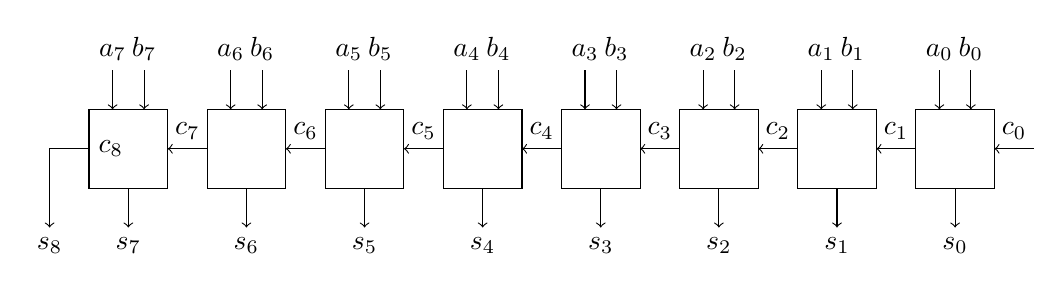
\begin{tikzpicture}[scale=0.5]
    \foreach \x [evaluate={\y=int(7-\x);\z=int(8-\x)}] in {0,1,...,7}
    {
        \draw (3*\x,0) rectangle (3*\x+2,2);
        \draw[->] (3*\x+1,0)  -- (3*\x+1,-1) node[anchor=north] {$s_\y$};
        \draw[->] (3*\x+3,1) -- node[midway,anchor=south] {$c_\y$} (3*\x+2,1);
        \draw[->] (3*\x+0.6,3) node[anchor=south] {$a_\y$} -- (3*\x+0.6,2) ;
        \draw[->] (3*\x+1.4,3) node[anchor=south] {$b_\y$} -- (3*\x+1.4,2) ;
    }
    \draw[->] (0,1) node[anchor=west] {$c_8$} -- (-1,1) -- (-1,-1) node[anchor=north] {$s_8$};
\end{tikzpicture}
}
\caption{}
\end{figure}

全加器接收三个输入$a,b,c_i$,其中$a,b$分别是两个加数,$c_i$是输入进位。全加器产生两个输出$s,c_o$,其中$s$是和,$c_o$是输出进位。全加器的真值表如\autoref{tab1819}。这个逻辑我们在\autoref{exa3}中已经讨论了。

\begin{table}[!ht]
\centering
\begin{tabular}{ccc|cc}
$a$&$b$&$c_i$&$c_o$&$s$\\\hline
0&0&0&0&0\\
0&0&1&0&1\\
0&1&0&0&1\\
0&1&1&1&0\\
1&0&0&0&1\\
1&0&1&1&0\\
1&1&0&1&0\\
1&1&1&1&1
\end{tabular}
\caption{全加器的真值表}\label{tab1819}
\end{table}

\begin{figure}[!ht]
\centering
\includegraphics{images/408.png}
\qquad
\includegraphics{images/409.png}
\caption{四位加法器。红线和蓝线分别表示两个加数,绿线为进位,黄线为和,底端绿线为溢出位。上面低位下面高位。}\label{fig37}
\end{figure}

有了全加器,直接把多个全加器首尾相连,就得到了一个加法器(\autoref{fig37})。这个加法器要求两个加数从低位到高位依次延迟一个逻辑帧输入。

\begin{figure}[!ht]
\centering
\includegraphics{images/410.png}
\qquad
\includegraphics{images/411.png}
\caption{四位累加器。两个加数依次输入红蓝线。上面低位下面高位。}\label{fig38}
\end{figure}

除了用组合逻辑,我们还可以用时序逻辑做加法器。降频电路有逢二进一的特性,所以可以直接用降频电路做一个加法器(\autoref{fig38})。与组合逻辑加法器不同,时序逻辑加法器实质上是累加器,如果不复位,那么每次输入都会直接累加到上一次的结果上。在时序逻辑加法器中,第二个加数各位要在同一个逻辑帧输入,或者低位延迟输入,这与组合逻辑加法器恰好相反。

在加法器上,时序逻辑的另一个优点是,把降频电路改成递次电路,就可以直接做任何进制的累加。\bilibili{av40474377/}中的进制转换实际上就是做了一个十进制累加器,每修改一个二进制数位就向累加器中加一个值或减一个值。

\subsection{减法器(Subtractor)}
有了补码这个工具,减法器和加法器就可以共用一个电路,我们只需要增加一些部件将其中一个加数取反加一。取反的操作是容易的,而加一的操作正好可以借用\autoref{tab1406}中我们没有用到的$c_0$。做出的组合逻辑加减法器如\autoref{fig39}所示,需要注意的是加法器的输入从低位到高位延迟一个逻辑帧,所以对每个数位取反的时候也要从低位到高位延迟一个逻辑帧,完成这项工作的是\autoref{fig39}中最右边一列逻辑门。

\begin{figure}[!ht]
\centering
\includegraphics{images/412.png}
\qquad
\includegraphics{images/413.png}
\caption{四位加减法器。顶端黄线控制加减法,0为加法,1为减法。计算加法时红线和蓝线分别表示两个加数。计算减法时蓝线为被减数,红线为减数。黄线为和,底端绿线为溢出位。上面低位下面高位。}\label{fig39}
\end{figure}

时序逻辑的减法器同样是使用补码运算,这里不给出具体实现。

\subsection{比较器(Comparator)}
比较两个数的大小,最简单的就是从高位向低位逐位比较。例如比较$a_{[7:0]}$和$b_{[7:0]}$两个8位二进制数,首先比较最高位$a_7$和$b_7$,如果它们相等再比较$a_6$和$b_6$,依此类推。最后我们可以得到一个逻辑表达式:
\[\begin{split}
a_{[7:0]}\mathtt{>}b_{[7:0]}=&(a_7\mathtt{>}b_7)(a_7\mathtt{==}b_7\& a_6\mathtt{>}b_6)(a_7\mathtt{==}b_7\& a_6\mathtt{==}b_6\& a_5\mathtt{>}b_5)\\
&(a_7\mathtt{==}b_7\& a_6\mathtt{==}b_6\& a_5\mathtt{==}b_5\& a_4\mathtt{>}b_4)\\
&(a_7\mathtt{==}b_7\& a_6\mathtt{==}b_6\& a_5\mathtt{==}b_5\& a_4\mathtt{==}b_4\& a_3\mathtt{>}b_3)\\
&(a_7\mathtt{==}b_7\& a_6\mathtt{==}b_6\& a_5\mathtt{==}b_5\& a_4\mathtt{==}b_4\& a_3\mathtt{==}b_3\& a_2\mathtt{>}b_2)\\
&(a_7\mathtt{==}b_7\& a_6\mathtt{==}b_6\& a_5\mathtt{==}b_5\& a_4\mathtt{==}b_4\& a_3\mathtt{==}b_3\& a_2\mathtt{==}b_2\& a_1\mathtt{>}b_1)\\
&(a_7\mathtt{==}b_7\& a_6\mathtt{==}b_6\& a_5\mathtt{==}b_5\& a_4\mathtt{==}b_4\& a_3\mathtt{==}b_3\& a_2\mathtt{==}b_2\& a_1\mathtt{==}b_1\& a_0\mathtt{>}b_0)
\end{split}\]
用\autoref{sec23}中的导出公式,我们得到了只包含初等布尔运算的逻辑表达式:
\[\begin{split}
a_{[7:0]}>b_{[7:0]}=&(a_7\&\textrm{\~{}}b_7)(\textrm{\~{}}a_7b_7\& a_6\&\textrm{\~{}}b_6)(\textrm{\~{}}a_7b_7\&\textrm{\~{}}a_6b_6\& a_5\&\textrm{\~{}}b_5)\\
					&(\textrm{\~{}}a_7b_7\&\textrm{\~{}}a_6b_6\&\textrm{\~{}}a_5b_5\& a_4\&\textrm{\~{}}b_4)\\
					&(\textrm{\~{}}a_7b_7\&\textrm{\~{}}a_6b_6\&\textrm{\~{}}a_5b_5\&\textrm{\~{}}a_4b_4\& a_3\&\textrm{\~{}}b_3)\\
					&(\textrm{\~{}}a_7b_7\&\textrm{\~{}}a_6b_6\&\textrm{\~{}}a_5b_5\&\textrm{\~{}}a_4b_4\&\textrm{\~{}}a_3b_3\& a_2\&\textrm{\~{}}b_2)\\
					&(\textrm{\~{}}a_7b_7\&\textrm{\~{}}a_6b_6\&\textrm{\~{}}a_5b_5\&\textrm{\~{}}a_4b_4\&\textrm{\~{}}a_3b_3\&\textrm{\~{}}a_2b_2\& a_1\&\textrm{\~{}}b_1)\\
					&(\textrm{\~{}}a_7b_7\&\textrm{\~{}}a_6b_6\&\textrm{\~{}}a_5b_5\&\textrm{\~{}}a_4b_4\&\textrm{\~{}}a_3b_3\&\textrm{\~{}}a_2b_2\&\textrm{\~{}}a_1b_1\& a_0\&\textrm{\~{}}b_0)
\end{split}\]

\begin{figure}
\centering
\includegraphics{images/396.png}\qquad\includegraphics{images/397.png}
\caption{逐位比较器。上方火把表示$b_{[7:0]}$,左边高位右边低位;右侧火把表示$a_{[7:0]}$,下方高位上方低位;左下火把表示$a_{[7:0]}\mathtt{>}b_{[7:0]}$。}\label{fig33}
\end{figure}
将这个逻辑表达式转换为电路如\autoref{fig33}所示。

比较两个数的大小,除了逐位比较之外,还可以直接将两个数做减法,并判断结果的正负性。减法器我们已经做过了,而补码表示中,一个数的正负可以直接通过最高位得出。这里有两个细节的问题。无符号整数没有符号位,如何比较两个无符号整数的大小?有符号整数的两数之差可以达到$127-(-128)=255=11111111$,而这个数作为有符号整数实际上表示$-1$,即小于0。如何处理这些特殊情况?事实上我们这里的比较器只能比较无符号整数,而所谓的“最高位”实际上指的是\autoref{tab1406}中的溢出位$s_8$。对于有符号整数有两种处理方法:第一种是首先判断符号,如果符号相等,再做无符号整数的比较;第二种是把两个数都加$128$,这样就把$-128\sim127$的范围变成了$0\sim255$,然后做无符号整数的比较即可。

比较两个数是否相等,也有两种解法,一种是直接逐位比较,另一种是判断它们的差是否为0。这两种方法并没有绝对的优劣,虽然逐位比较的电路会比较简单,但是判断差值的电路可以直接附加在其他功能上,例如加法器。

\subsection{乘法器(Multiplier)}
乘法是加法的推广,乘法器也是加法器的推广。我们首先来看二进制乘法的竖式计算。因为乘法规模较大,这里给出4位乘法的例子(\autoref{tab6585})。

\begin{figure}[!ht]
$$
\begin{array}{ccccccccc}
&&&&a_3&a_2&a_1&a_0\\
&&&&b_3&b_2&b_1&b_0\\\hline
&&&&b_0\&a_3&b_0\&a_2&b_0\&a_1&b_0\&a_0\\
&&&b_1\&a_3&b_1\&a_2&b_1\&a_1&b_1\&a_0\\
&&b_2\&a_3&b_2\&a_2&b_2\&a_1&b_2\&a_0\\
&b_3\&a_3&b_3\&a_2&b_3\&a_1&b_3\&a_0\\\hline
H_3&H_2&H_1&H_0&l_3&l_2&l_1&l_0
\end{array}
$$
\caption{乘法竖式计算}\label{tab6585}
\end{figure}

从\autoref{tab6585}可以看出来,做一个4位乘法实际上就是做4个数的加法。4个数的加法,可以按照运算顺序拆分成三次2个数的加法,如\autoref{fig79}所示。

\begin{figure}[!ht]
\centering
\begin{tikzpicture}
    \draw (0,0) rectangle node{加法器} (5,1);
    \draw (0,2) rectangle node{加法器} (5,3);
    \draw (0,4) rectangle node{加法器} (5,5);
    
    \draw[->] (2,6) node[anchor=south]{$a_1$} -- (2,5);
    \draw[->] (3,6) node[anchor=south]{$a_2$} -- (3,5);
    \draw[->] (2,4)  -- node[midway,anchor=east]{$a_1+a_2$} (2,3);
    \draw[->] (6,3.5) node[anchor=west]{$a_3$} -- (3,3.5) -- (3,3);
    \draw[->] (2,2)  -- node[midway,anchor=east]{$a_1+a_2+a_3$} (2,1);
    \draw[->] (6,1.5) node[anchor=west]{$a_4$} -- (3,1.5) -- (3,1);
    \draw[->] (2.5,0) -- (2.5,-1) node[anchor=north]{$a_1+a_2+a_3+a_4$};
\end{tikzpicture}
\caption{四个加数$a_1,a_2,a_3,a_4$连加}\label{fig79}
\end{figure}

把\autoref{fig79}中的加法器展开成串联的全加器,就得到了四位乘法器的结构示意图(\autoref{fig80})。

\begin{figure}[!ht]
\centering
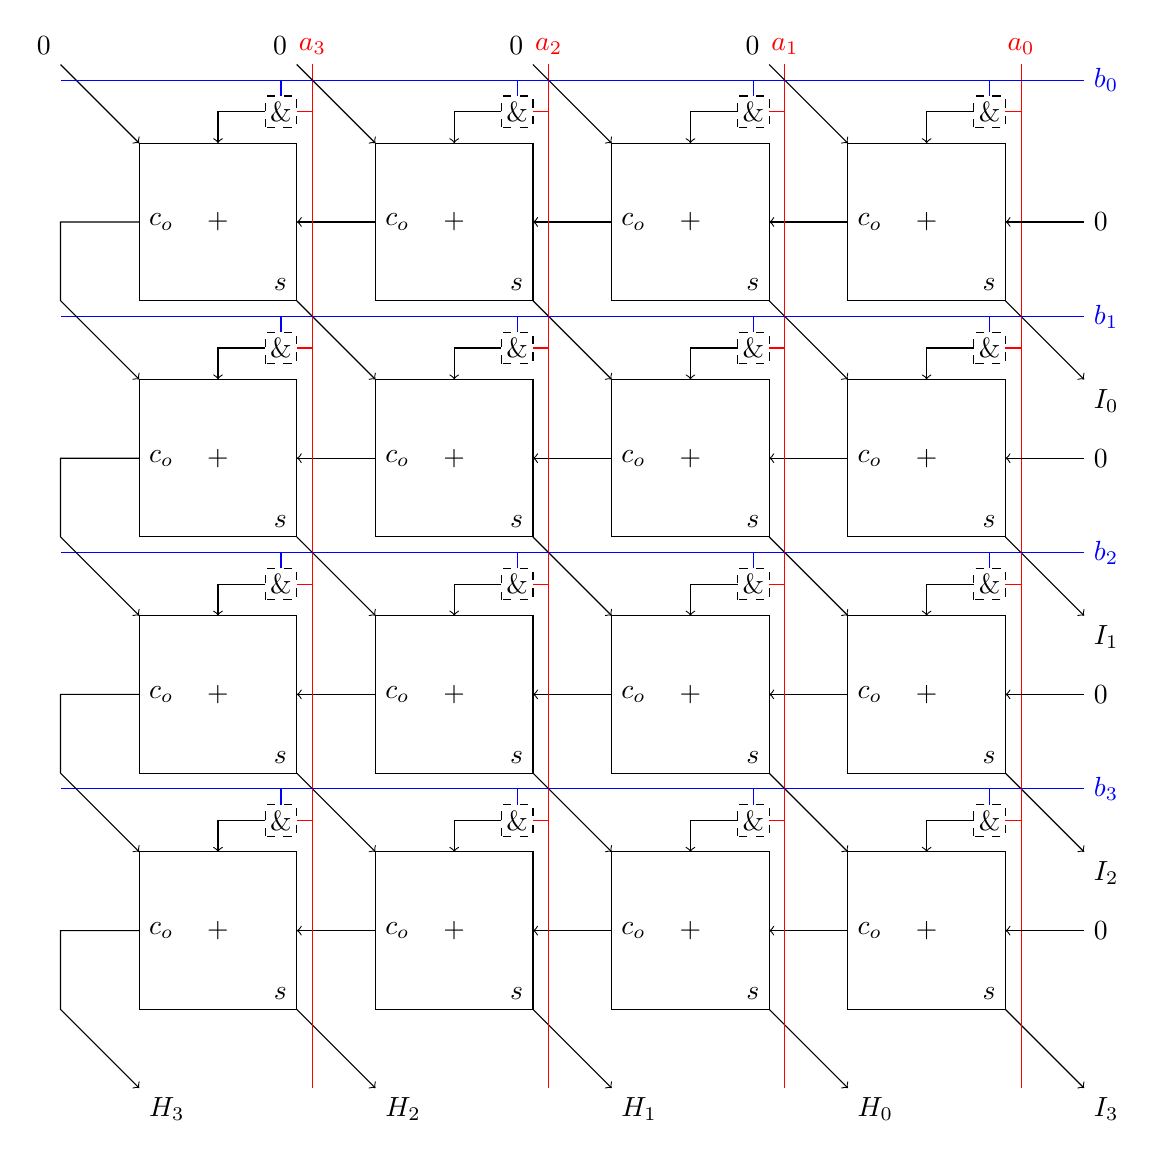
\begin{tikzpicture}
    \foreach \x [evaluate={\z=int(3-\x)}] in {0,1,2,3}
        \foreach \y [evaluate={\w=int(3-\y)}] in {0,1,2,3} {
            \draw (3*\x,3*\y) rectangle node {$+$} (3*\x+2,3*\y+2); % 全加器框架
            \draw[dashed] (3*\x+1.6,3*\y+2.2) rectangle node {\&} (3*\x+2,3*\y+2.6);
            \draw[->] (3*\x+1.6,3*\y+2.4) -- (3*\x+1,3*\y+2.4) -- (3*\x+1,3*\y+2);
            \draw[blue] (3*\x+1.8,3*\y+2.6) -- (3*\x+1.8,3*\y+2.8);
            \draw[red] (3*\x+2,3*\y+2.4) -- (3*\x+2.2,3*\y+2.4);
            \draw[->] (3*\x+2,3*\y) node[anchor=south east] {$s$} -- (3*\x+3,3*\y-1); % 和输出
        }
    \foreach \x in {1,2,3}
        \foreach \y in {0,1,2,3}
            \draw[->] (3*\x,3*\y+1) node[anchor=west] {$c_o$} -- (3*\x-1,3*\y+1); % 进位连接
    \foreach \x [evaluate={\z=int(3-\x)}] in {0,1,2,3}{
        \draw[->,] (3*\x-1,12) node[anchor=south east] {$0$} -- (3*\x,11); % 第一排缺省加数
        \draw (3*\x,-1) node[anchor=north west] {$H_\z$}; % 结果高四位
        \draw[red] (3*\x+2.2,12) node[anchor=south] {$a_\z$} -- (3*\x+2.2,-1); %乘数1输入
    }
    \foreach \y [evaluate={\w=int(3-\y)}] in {0,1,2,3}{
        \draw (12,3*\y-1) node[anchor=north west] {$I_\w$}; % 结果低四位
        \draw[->] (0,3*\y+1) node[anchor=west] {$c_o$} -- (-1,3*\y+1) -- (-1,3*\y) -- (0,3*\y-1); % 左边一列进位输出
        \draw[->] (12,3*\y+1) node[anchor=west] {$0$} -- (11,3*\y+1); % 右边一列进位输入
        \draw[blue] (12,3*\y+2.8) node[anchor=west] {$b_\w$}-- (-1,3*\y+2.8); % 乘数2输入
    }
\end{tikzpicture}
\caption{四位乘法器结构示意图。大的实线方框表示全加器,$c_o$表示进位输出,$s$表示和输出。小的虚线方框表示与门,红蓝线输入,黑线输出。两个乘数分别从上方和右方输入,乘积的低位从右边输出,高位从下边输出。全加器缺少的输入补零。左右相邻的两个全加器,右边的早一个逻辑帧;上下相邻的两个全加器,上边的早两个逻辑帧。}\label{fig80}
\end{figure}

乘法器的单个单元电路见\autoref{fig81},其中用不同颜色的背景墙标记区域和线路。橙色区域为全加器。黄色区域是与门。蓝色线路是从右边输入的乘数,每经过一个单元要延迟1个逻辑帧。红色线路是从上边输入的乘数,每经过一个单元要延迟2个逻辑帧。紫色线路是横向的进位传递。绿色线路是从左上到右下的和传递。

\begin{figure}[!ht]
\centering
\includegraphics{images/436.png}
\caption{乘法器单个单元的结构}\label{fig81}
\end{figure}

单元堆叠后的效果见\autoref{fig82},其中每个单元大小3*7。优化过程用到了如下的接线技巧:
\begin{itemize}
	\item 左右方向上红蓝线循环,便于接线。
	\item 相邻两列错位,便于进位和横向乘数的传递。
	\item 纵向的逻辑延迟用到了一个异或门,从而这个门不需要为经过的绿线让路。
	\item 与门利用了等式$a\&b=\textrm{\~{}} ab\&b$,便于接线。
\end{itemize}

\begin{figure}[!ht]
\centering
\includegraphics[width=\textwidth]{images/437.png}
\caption{堆叠优化后的效果}\label{fig82}
\end{figure}

\subsection{除法器(Divider)}
1
\subsection{移位器(Shifter)}
移位又分为逻辑移位、算术移位、循环移位,其中逻辑移位和算术移位应用较广。

\begin{figure}[!ht]
\centering
\subfloat[逻辑右移一位]{\includegraphics{images/414.png}}
\qquad
\subfloat[算术右移一位]{\includegraphics{images/415.png}}
\qquad
\subfloat[循环右移一位]{\includegraphics{images/416.png}}
\caption{递次电路移位}\label{fig40}
\end{figure}

如果只移一位的话,这三种移位都可以通过递次电路实现,如\autoref{fig40}所示。

\begin{figure}
\centering
\subfloat[逻辑右移]{\includegraphics[width=0.45\textwidth]{images/400.png}\qquad\includegraphics[width=0.45\textwidth]{images/401.png}}

\subfloat[算术右移]{\includegraphics[width=0.45\textwidth]{images/402.png}\qquad\includegraphics[width=0.45\textwidth]{images/403.png}}

\subfloat[经过简单优化的算术右移]{\includegraphics[width=0.45\textwidth]{images/404.png}\qquad\includegraphics[width=0.45\textwidth]{images/405.png}}
\caption{组合逻辑原理的移位器。右侧三个火把从上到下作用依次为移1位、移2位、移4位。}\label{fig35}
\end{figure}

如果要移任意位,递次电路大概率会爆门,此时需要考虑其他方案。一个简单的思路是使用\autoref{fig35}所示的组合逻辑。这个组合逻辑的缺点是,被移位数的所有数位输入要在同一个逻辑帧,而移位量的数位要在各个逻辑帧依次输入,调节逻辑同步较复杂。此外,由于逻辑门的取向问题,这种方法不适用于循环移位。

\begin{figure}[!ht]
\centering
\includegraphics{images/417.png}
\qquad
\includegraphics{images/418.png}
\caption{移位器。纵向的红蓝线输入待移位的数。横向红蓝线输入移位的位数。通过顶端的逻辑灯激活对应的输出。底端绿线用于切换逻辑移位和算术移位。}\label{fig41}
\end{figure}

事实上,因为数字电路结构都相对复杂,在泰拉瑞亚中想做一定规模的数字电路,一定要考虑利用\nameref{sec17}技术传输数据。\nameref{sec17}技术通过在不同逻辑帧发送不同数位传播数据,我们可以通过这一特点设计专门兼容\nameref{sec17}的移位器。\autoref{fig41}通过选取网线输出的起始数位实现移位功能。

\subsection{随机数生成器(Random Number Generator)}
在现实中需要用复杂算法实现的功能,在泰拉瑞亚中反而异常简单。直接使用8个1/2概率的故障逻辑门,我们就可以随机生成8位二进制数。
\vspace{5cm}

没了。

\subsection{进制转换}

\paragraph*{方法一} 直接用定义式$a_{n:0}=a_n2^n+a_{n-1}2^{n-1}+\cdots+a_02^0$。要利用这个式子将二进制转换为十进制,需要做一个十进制加法器,然后存储2的各次幂的十进制值。\url{https://www.bilibili.com/video/av40474377/}就是用的这种方法。

十进制转二进制可以用同样的原理,做一个二进制加法器,然后存储10的各次幂的二进制值。

\paragraph*{方法二} 利用\autoref{sec30}和\autoref{sec31}介绍的方法。在竖式的每一步中,我们需要做一个查表的操作,然后错一位。这个查表的操作实际上是一个组合逻辑,如\autoref{tab12}所示。

\begin{table}[!ht]
\centering
\begin{tabular}{|c|c|}
\hline
二进制&BCD\\\hline
0000&0000\\\hline
0001&0001\\\hline
0010&0010\\\hline
0011&0011\\\hline
0100&0100\\\hline
0101&1000\\\hline
0110&1001\\\hline
0111&1010\\\hline
1000&1011\\\hline
1001&1100\\\hline
\end{tabular}
\caption{二进制转BCD则从左到右查,BCD转二进制则从右到左查。}\label{tab12}
\end{table}

二进制转BCD和BCD转二进制对应不同的真值表,我们需要分开设计。

\section{存储电路}
一个存储电路总是要有一个用于存放数据的阵列和一个选择数据的多路选择器。

\subsection{多路选择器(Multiplexer)}
多路选择器接收一个二进制地址,激活该地址代表的位置。一个经典的四位多路选择器如\autoref{fig42}所示。

\begin{figure}[!ht]
\centering
\includegraphics{images/419.png}\vspace{16pt}

\includegraphics{images/420.png}
\caption{经典四位多路选择器。红蓝线表示地址,上面高位下面低位。绿线双激活输出。16个逻辑门从左到右依次表示0000到1111。}\label{fig42}
\end{figure}

我们在\nameref{sec2:2}中曾见过相似的电路,事实上那个就是状态版的多路选择器。本小节中我们通过\nameref{sec33}实现了激活版的多路选择器。

\subsection{只读存储器(Read-Only Memory)}
只读存储器用于存储事先设计好的、固定的数据。这些数据不需要在使用时修改,所以一般是通过物理方式直接做在电路中。
\begin{figure}[!ht]
    \centering
	\subfloat[横向输入纵向输出]{\label{fig49}\includegraphics{images/342.png}\quad\includegraphics{images/341.png}}
    \qquad
	\subfloat[纵向输入横向输出]{\label{fig50}\includegraphics{images/343.png}\quad\includegraphics{images/344.png}}
    \qquad
	\subfloat[纵向输入横向输出]{\label{fig51}\includegraphics{images/346.png}\quad\includegraphics{images/345.png}}
    \caption{ROM的三种设计。}\label{fig48}
\end{figure}
\autoref{fig48}展示了三种ROM设计。\autoref{fig49}使用故障逻辑灯存储数据。一根横线激活时,只有经过的故障逻辑灯下方的逻辑门才会激活。因为存储器要与多路选择器配合,而多路选择器是纵向输出,所以\autoref{fig49}目前没有实用价值。\autoref{fig50}和\autoref{fig51}都是通过接线存储数据,也是有广泛应用的两种ROM。两个电路在实现方式上的区别是,\autoref{fig50}通过连接输出线与逻辑门来存储,而\autoref{fig51}通过连接输入线与逻辑灯来存储。占用空间方面,\autoref{fig50}占用高度较低(1.5格/bit),\autoref{fig51}占用高度较高(2格/bit)。逻辑同步方面,\autoref{fig51}的输出是同步的,而\autoref{fig50}不同步,在本来就需要不同步的场景(例如很多\nameref{sec34}和\nameref{sec17}),\autoref{fig50}更好。

\nameref{sec2:2}中,\autoref{i36:37}就是状态式的多路选择器,\autoref{i42:43}的下半部分电路就是\autoref{fig50}样式的ROM。只有有限个输出情况的显示器都可以通过ROM实现。

\subsection{只写存储器(Write-Only Memory)}
1
\subsection{随机存储器(Random Access Memory)}
1
\subsection{寄存器(Register)}
1
\subsection{栈(Stack)}
1

\section{分段显示器化简理论}
1
\subsection{分段显示器主要结构}
1
\subsection{显示矩阵、分段矩阵和数字矩阵}
1
\subsection{矩阵的初等变换}
1
\subsection{化简原理与细节}
1

\section{处理器结构}
1
\subsection{汇编语言}
1
\subsection{机器语言}
1
\subsection{处理器的拓扑结构}
1
\subsection{数据路径(Data Path)}
1
\section{电源详解}\label{sec1}

\subsection{开关/控制杆}
开关和控制杆的激活条件是鼠标右击。同其他交互类物品/NPC相同,只有当开关/控制杆在可触及范围内时才可以右击。

与控制杆相比,由于开关体积更小,在电路密集时一般都使用开关。另一方面,小的体积带来的缺点是开关不容易发现,而且容易点错。

开关可以放置在木梁侧面与前景物块侧面而控制杆不行;控制杆可以放置在平坦表面上而开关不行(\autoref{i204})。需要注意的是,只有当砧上有足够面积的背景墙时,控制杆才可以放置在砧上,放置在砧上后敲掉背景墙也不会掉落,这可能是判定的bug。

\begin{figure}[!ht]
\centering
\includegraphics[width=0.9\textwidth]{images/204.png}
\caption{放置在平坦表面上的控制杆}
\label{i204}
\end{figure}

\subsection{压力板}
压力板分为普通压力板、加重压力板、青绿压力垫板。

普通压力板包括由玩家触发的灰/棕/蓝/丛林蜥蜴压力板、由敌怪触发的黄压力板和由玩家或敌怪触发的红/绿压力板。加重压力板是误翻译,正确翻译应为“重力压力板”。四种颜色的加重压力板功能完全一样。

普通压力板有自身的碰撞箱,碰撞箱大小是压力板弹起状态时贴图的边框大小。普通压力板激活的判定以每个碰撞箱为准,即每帧判定碰撞箱是否从侧面进入压力板,或从上面掉落到压力板上。因为是以碰撞箱为准,所以一个碰撞箱在一帧内触发两个普通压力板,只会激活一次,而不同碰撞箱在一帧内触发同一个普通压力板,每个碰撞箱都会激活一次(\autoref{i205:208})。注意到“进入”或“掉落”都是过程,所以直接传送到普通压力板上不会触发压力板。同时,“掉落”要求人物有一个悬空的过程,判断悬空可以通过人物动作(悬空时有跳跃动作)或者翅膀(装备了翅膀的人物悬空时翅膀会打开)。所以从1格高的物块上直接走下来不算掉落,同时碰撞箱也不是从侧面进入,所以不会触发普通压力板(\autoref{i201:202})。

\begin{figure}[!h]
\begin{center}
\subfloat[]{
\label{i205:206}
\includegraphics{images/205.png}
\includegraphics{images/206.png}
}
\qquad
\subfloat[]{
\label{i207:208}
\includegraphics{images/207.png}
\includegraphics{images/208.png}
}
\end{center}
\caption{\protect\subref{i205:206}同时踩踏两个红压力板,只有左边的火把响应;\protect\subref{i207:208}虚化两个NPC脚下的方块,两个NPC同时掉落到红压力板上,火把仍亮。}
\label{i205:208}
\end{figure}

\begin{figure}[!h]
\begin{center}
\subfloat[]{
\label{i201}
\includegraphics{images/201.png}
}
\qquad
\subfloat[]{
\label{i202}
\includegraphics{images/202.png}
}
\end{center}
\caption{\protect\subref{i201}直接从一格高度走下,翅膀不打开,无跳跃动作,压力板不会被触发;\protect\subref{i202}在平台上按“下”方向键,翅膀打开,有跳跃动作,压力板会被触发。}
\label{i201:202}
\end{figure}

加重压力板没有碰撞箱,判定以压力板本身为准,即每帧或者每次传送后判定是否有人物在压力板所在格内,直接传送到加重压力板上可以触发加重压力板。为避免冲突,加重压力板的激活信号及以该信号触发的逻辑结算产生的激活信号不会触发传送机。

青绿压力垫板的碰撞箱为16*10或10*16,根据其朝向而定。射弹生成后,每次更新位置都会激活碰撞到的青绿压力垫板,这里碰撞的定义是:上次更新时碰撞箱不相交,但是这次更新时相交。如果射弹同时与多个青绿压力垫板碰撞,那么只激活优先级最高的那个(不同行的青绿压力垫板,上面的优先级高;同一行的青绿压力垫板,左边的优先级高);多个射弹同时碰撞同一个青绿压力垫板,每个射弹都会激活一次(\autoref{i209:212})。

\begin{figure}[!h]
\begin{center}
\subfloat[]{
\label{i209:210}
\includegraphics{images/209.png}
\includegraphics{images/210.png}
}
\qquad
\subfloat[]{
\label{i211:212}
\includegraphics{images/211.png}
\includegraphics{images/212.png}
}
\end{center}
\caption{\protect\subref{i209:210}大炮发射,只有左边的火把响应;\protect\subref{i211:212}激活左边或右边的开关火把都响应,激活中间的开关火把不响应(实际上响应了两次)。}
\label{i209:212}
\end{figure}

普通压力板和加重压力板可以放在平台和锭上而青绿压力垫板不能;青绿压力垫板可以放在前景物块侧面和下方而普通压力板和加重压力板不能。

压力板轨道是带有压力板的轨道,它只能由矿车触发。

\subsection{引爆器}
引爆器是一个比较特殊的物品,其有压下和弹起两种状态。鼠标右击或人物以至少3像素/帧的垂直速度经过引爆器上两格时会导致引爆器压下并作为电源激活,随后经过1秒,引爆器自动弹起。可能出于判定原因,当人物以一定速度(既不快也不慢)落在引爆器旁边的支撑物边缘时引爆器也会压下(\autoref{i213:214})。引爆器处于压下状态时鼠标右击或人物踩踏均无效(贤者模式)。

\begin{figure}[!h]
\begin{center}
\subfloat[]{
\label{i213}
\includegraphics{images/213.png}
}
\qquad
\subfloat[]{
\label{i214}
\includegraphics{images/214.png}
}
\end{center}
\caption{\protect\subref{i213}站在平台边缘原地跳跃,当跳跃高度在某个范围内时,落下会踩下引爆器;\protect\subref{i214}骑乘坐骑也有这种现象。}
\label{i213:214}
\end{figure}

引爆器同样也是用电器,被激活时会在压下和弹起之间切换。如果引爆器被激活压下,那么不会作为电源激活,也不会自动弹起,直到再次被激活弹起。

引爆器可以放在几乎所有平坦表面上。与控制杆不同的是,引爆器不是悬挂家具,所以不能放在砧上。

\subsection{受困宝箱}
受困宝箱是误翻译,正确翻译应该是“机关宝箱”或“陷阱宝箱”。受困宝箱是电源,当鼠标右击时激活并播放宝箱开启关闭的动画。除了右击效果不同以外,受困宝箱与对应的普通宝箱外观、放置方式完全相同,这使得受困宝箱可以用来做陷阱的触发器。

\subsection{感应器}
泰拉瑞亚中共有3种逻辑感应器和4种液体感应器。逻辑感应器(昼)在白天点亮,夜晚熄灭;逻辑感应器(夜)在白天熄灭,夜晚点亮;逻辑感应器(玩家)放置时对应一个电路层的蓝色方框,该方框宽略大于5格,高略大于10格,当框内有玩家时感应器点亮,当框内无玩家时感应器熄灭。液体感应器在所在格中有对应液体时点亮,无对应液体时熄灭。

逻辑感应器(昼)和逻辑感应器(夜)在由灭变亮时激活,其他感应器均在亮灭切换时激活。

逻辑感应器(玩家)可以看作感应范围更大,但是对传送不敏感,仅在每帧进行判断的加重压力板。逻辑感应器(玩家)的激活信号及以该信号触发的逻辑结算产生的激活信号不会触发传送机。

所有感应器均可随意放置,无需支撑块或背景墙。

使用地图编辑器或Mod复制粘贴的感应器无法工作,需拆除后手动放置。因此设计电路时应尽量避免大规模使用感应器。

\subsection{其他电源}
剩余的电源在wiki之外的信息相当少,因此不专门介绍。它们是:计时器、宝石锁。

\section{用电器详解}\label{sec4}

\subsection{部分光源}
这里说的光源不是指有效光源,而是指所有能发光的物体。所有可由电路控制的光源如下列举。

\begin{itemize}
\item 火把:大小1*1,放置在平台上、前景物块上方和两侧、背景墙上。是有效光源。
\item 蜡烛:大小1*1,放置在除砧以外的平坦表面上,可以放置在锭上但会立刻掉落。水蜡烛和和平蜡烛无电路功能。是有效光源。
\item 灯笼:大小1*2,悬挂在前景物块下。萤火虫瓶和荧光虫瓶无电路功能。星星瓶和红心灯笼熄灭时不提供buff。是有效光源。
\item 灯:大小1*3,放置在平台上、锭上、前景物块上。是有效光源。
\item 篝火:大小3*2,放置在平台上、锭上、前景物块上。熄灭时不提供buff。是有效光源。
\item 烛台:大小2*2,放置在除砧以外的平坦表面上、前景物块上。是有效光源。
\item 吊灯:大小3*3,悬挂在前景物块下。是有效光源。
\item 晶莹宝石块:属于前景物块。不是有效光源。
\item 中式灯笼:大小2*2,悬挂在前景物块下。是有效光源。
\item 灯柱:大小1*6,放置在平台上、锭上、前景物块上。不是有效光源。
\item 迪斯科灯:大小2*2,悬挂在前景物块下。不是有效光源。
\item 圣诞灯:大小1*1,放置在前景物块四周。是有效光源。
\item 壁炉:大小3*2,放置在平台上、锭上、前景物块上。是有效光源。
\end{itemize}

这里需要强调一下常用的两种显示光源:宝石块和火把。一般情况下宝石块显示效果更好,并且其亮灭会显示在小地图中。然而由于火把激活时只是简单改变状态,而每个宝石块激活时还需要更新该块及周围8块的贴图,每次更新贴图时都需要进行大量的判断,这导致大规模使用宝石块的电路与使用火把的电路相比非常卡。

\subsection{门、机关门、高门}
上锁的丛林蜥蜴门无电路功能(废话)。门放置在上下两个前景物块之间。图格、生物出现在门一侧的开启范围内(1*3)时门不会向这一侧开启;出现在门两侧开启范围内时门无法开启。当门可以向两侧开启时,如果右键开门,那么门向玩家面对方向开启;如果电路开门,那么门似乎是随机向两侧开启。

与门相比,机关门的开启方向是上下。当机关门可以向两侧开启时,使用右键开门,根据玩家与门的相对位置确定开门方向:玩家在相对高处时门向下开启;玩家在相对低处时门向上开启。使用电路开门,固定向下开启。

高门没有方向性,开门也不受阻挡。

\subsection{泵}
用一根电线连接一个入水泵和一个出水泵,则电线激活时,入水泵上的液体会尽可能多的转移到出水泵。

为了了解一些奇怪情况下的液体转移结算,这里介绍水泵的内部运行机制。

游戏中用两个长度19的列表分别存储入水泵和出水泵的坐标。在这个列表中,每个泵都是单个图格。游戏中的泵包含四个图格,当该泵被激活时,四个图格被依次加入列表中,顺序是左下-右下-左上-右上。加到列表满时则不继续加入。

每根电线结算完成后进行水泵结算,从前往后扫描入水泵列表(没有液体的入水泵除外),对于每个入水泵,从前往后扫描出水泵列表(满液体的出水泵除外),并对入水泵和出水泵中的液体进行转移。

单格入水泵和单格出水泵之间的液体转移,首先要遵循液体一致的原则,即转移液体不会导致不同液体出现在出水泵上。其次,转移的量为入水泵上的液体总量和出水泵上空余液体量的最小值(每格中的液体量为0到255)。

\subsection{机关}
这里说的机关指激活会对玩家造成伤害的用电器。

超级飞镖机关、尖球机关、烈焰机关、长矛机关都生成在丛林蜥蜴神庙内。飞镖机关生成在地下其他位置。这5种机关属于前景物块,锤击可以改变射击方向;被激活会生成射弹,可触发青绿压力垫板。

飞镖机关、超级飞镖机关、尖球机关和烈焰机关的射弹在机关前方第2格生成,因此紧贴这4种机关前方的一个前景物块不会阻挡射弹。紧贴长矛机关前方的前景物块会阻挡长矛。

飞镖在真空中的速度是每秒45格,生存时间60秒。飞镖机关、超级飞镖机关和烈焰机关的冷却时间是200帧。

长矛机关射程19.5格\footnote{由@dcfhft 验证。},冷却时间90帧。

烈焰机关射程20格,冷却时间200帧。尽管烈焰机关的特效较宽,其射弹仍只在机关正前方生成。

尖球机关冷却时间300帧,有生成限制。其限制规则较复杂,请参阅wiki。

因为翻译原因,喷泉(机关)在中文wiki中无法查到,因为与喷泉(装饰)冲突\footnote{喷泉(Geyser)是自然景观,喷泉(Fountain)是人造景观,官中并未区分翻译。}。请在英文wiki中查阅Geyser词条。

喷泉(机关)可放置在前景物块上或下,其朝向也根据放置位置分为朝上和朝下。冷却时间200帧。不会触发青绿压力垫板。射程20格,射程从喷射方向29格内遇到的第一个2*4开放空间(没有前景物块和液体)开始,其后会被障碍物阻挡。

炸药被激活时爆炸,爆炸半径10格。炸药是一次性的,所以在电路中应用有限。使用地图编辑器或Mod可以将炸药放在宝箱下,由于宝箱下的物块无敌,炸药可以被无限引爆。

地雷被激活时爆炸。与炸药的区别是地雷不破坏图格,伤害也更低。另一方面,地雷被玩家或NPC踩踏时也会爆炸,这使得引爆地雷可以不用电线,因此可以通过刷漆使地雷完全不可见。

\subsection{炮台}
炮台包括大炮、兔兔炮、彩纸炮、传送枪站和雪球发射器。

炮台大小为4*3,但是可以放置在两格宽的前景物块、平台或锭上。

鼠标右击炮台左/右部分可转向,拿着对应炮弹左击可发射。使用电线激活时,激活炮台的不同位置有不同效果(\autoref{i215})。使用电线激活发射的炮弹不造成伤害。

炮台生成射弹的位置横坐标在中间两列的交界,纵坐标在下面一格与中间一格的交界。对于传送枪台,生成位置还要向下移5像素;如果传送枪台朝向垂直向上,生成位置还要向右移5像素。

炮台生成射弹的初速度大小,传送枪站为93像素/帧\footnote{具体为每次前进3像素,每帧前进31次},其他为14像素/帧。初速度方向只与炮台朝向有关,除了0、$\pi/2$、$\pi/4$的特殊角以外,非特殊角分别为$\arctan(1/3)$和$\pi/2-\arctan(1/3)$而不是$\pi/8$和$3\pi/8$。

大炮和兔兔炮的炮弹射出后,前17帧速度不变,从第18帧开始,每帧纵向速度增加0.28像素/帧(最大16像素/帧),横向速度乘0.99。传送枪台的射弹匀速直线运动,并会按顺序激活路径上的所有青绿压力垫板。彩纸炮发射的射弹匀速直线运行,生存期为2帧,生存期结束后爆炸,生成特效。在这2帧内,射弹只能前进28像素,无法离开炮台4*3的大小,也就无法触发青绿压力垫板。

\begin{figure}[!h]
\centering
\includegraphics{images/215.png}
\caption{红线右转,蓝线左转,绿线发射,黄线改变射弹颜色。}
\label{i215}
\end{figure}

传送枪站的鼠标操作与其他炮台不同。鼠标右击传送枪站不同位置效果与电线激活对应位置相同。

除彩纸炮以外的炮台发射的射弹可以触发青绿压力垫板。冷却时间30帧。

雪球发射器较特殊,其特性与以上描述几乎完全不同。雪球发射器大小3*3,只能放置在三格宽的前景物块、平台或锭上。雪球发射器不可手动转向,背包中有雪球时右击可发射雪球,可连发。发射出的雪球可触发青绿压力垫板。使用电路激活其左三格之一会使其朝向左,激活其右三格之一会使其朝向右,激活中间三格之一会发射不造成伤害的雪球。雪球发射器朝向只有两种:水平向左和水平向右。发射点在雪球发射器中心向左12像素(如果朝向左)或向右12像素(如果朝向右);发射速度在[12:0.01:16.49]中随机;发射方向随机(见\autoref{e1})。雪球发出后,前19帧速度不变,从第20帧开始,每帧纵向速度增加0.3(最大16),横向速度乘0.98。冷却时间10帧。

\begin{figure}[h]
\centering
\includegraphics[width=0.9\textwidth]{images/1.eps}
\caption{雪球发射器的发射方向。O为发射点,在如图所示矩形内随机取一点M,则OM为发射方向。}\label{e1}
\end{figure}

\subsection{烟花火箭}
烟花神教主角。关于烟花火箭的信息请参考wiki和\url{https://www.bilibili.com/video/av5050255}。

\subsection{传送机}\label{chuansongji}
一个传送机分为三个图格。传送机为前景物块,可以敲成半砖。传送机的工作机制中,三个图格分别有自己的传送区域(\autoref{i216})。

\begin{figure}[!h]
\centering
\includegraphics{images/216.png}
\caption{三个图格的传送区域。如果图格被敲成下半砖,则传送区域下移半格,其他半砖形态传送区域不变。}
\label{i216}
\end{figure}

当一根电线激活时,记录下该电线下第一个结算的传送机图格与最后一个结算的传送机图格\footnote{同一根电线上的结算顺序请参阅\autoref{jiesuanshunxu}},然后将两个图格传送区域内的可传送目标互换,互换后它们的速度不变,位置相对于传送区域不变。当两个图格的传送区域有重合并且第一个图格不低于最后一个图格时无法传送\footnote{这解释了为什么传送机不会自身传送。};当两个图格的传送区域有重合并且第一个图格低于最后一个图格时可以传送,此时两传送区域重叠部分属于第一个图格的传送区域(\autoref{i217:218})。

\begin{figure}[!ht]
\begin{center}
\subfloat{
\label{i217}
\includegraphics[width=0.9\textwidth]{images/217.png}
}
\qquad
\subfloat{
\label{i218}
\includegraphics[width=0.9\textwidth]{images/218.png}
}
\end{center}
\caption{左上装置:右边传送机比左边传送机传送区域高半格,因此玩家从左边传送到右边会高半格。中上装置:只要碰撞箱与传送区域有一点重叠,就可以传送。右上装置:传送机的三个图格各自有传送区域,从左边传送到右边,激活绿线会高半格,而激活蓝线红线不会。下方三个装置:激活上面开关不会传送,激活下面开关会传送;传送时只要玩家在下方传送机的传送区域内,就会被从下传到上;传送时只有玩家在上方传送机的传送区域内并且不在下方传送机的传送区域内,才会被从上传到下。}
\label{i217:218}
\end{figure}

\subsection{像素盒}
像素盒可随意摆放,无需支撑块或背景墙。像素盒有十字状态的分线盒的分线效果。当一个电源激活时,该电源上的所有电线激活,此时如果像素盒上有横向电线激活且无纵向电线激活,那么像素盒熄灭;如果像素盒上既有横向电线激活又有纵向电线激活,那么像素盒点亮;如果无横向电线激活,那么像素盒不响应。

需要注意的是,像素盒的响应是对电源敏感的,即分别结算每个电源发出的信号,这与传送机对电线敏感不同。同时,与一般的光源在亮灭之间切换不同,像素盒响应总是调整到对应状态。

\subsection{矿车轨道交叉点}
交叉点上必须有两个方向的平滑轨道,那么这两个平滑轨道必定是一个覆盖另一个,此时激活交叉点会使两个平滑轨道的覆盖关系改变。需要注意的是激活交叉点可以产生的变化数量远远小于使用锤子可以产生的变化数量。

\subsection{其他用电器}
剩余的用电器在wiki之外的信息相当少,因此不专门介绍。它们是:雕像、烟花喷泉、烟花盒、泡泡机、呆萌气球机、派对中心、喷泉、八音盒、烟囱、天塔柱、广播盒、制动器、传送带、彩线灯泡、增速轨道。
%\chapter{电路文档}

在前面章节中介绍电路的目的是帮助读者理解电路原理,所以有些电路仅给出了最简单的例子。在本章中,会直接给出一些电路的结果供参考。对于较难的电路会给出思路。

\section{传感器}
\subsection{重生感应器}
\subsection{开服感应器}
\subsection{血月感应器}
\subsection{雨天感应器}
\subsection{击退感应器}

\section{递次电路}
\subsection{传统递次电路}
\subsection{传统双向递次电路}
\subsection{多级递次电路}
\subsection{推广递次电路}

\section{降频电路}
\subsection{固定数值的降频}
\subsection{可变数值的降频}

\section{数字显示}
\subsection{BCD数显}
\subsection{十进制计数器}
\subsection{六进制计数器}
\subsection{月相显示}

\section{随机电路}
\subsection{随机多选一}
\subsection{随机分两组}
\subsection{随机分多组}

\section{操纵板}
\subsection{高频操纵板}
\subsection{低频操纵板}

\section{像素盒显示器}

\section{算术电路}
\subsection{加减乘除}
\subsection{状态位运算}
\subsection{激活位运算}
\subsection{移位}
\chapter{更多电路专题}

在前面我们已经学习了所有电路原理。在这一章中我们以电路功能分类,介绍一些常用的电路模块。当然在这之前,我们需要详细地了解泰拉瑞亚中所有电路物品的性质,这样才能知道我们可以做什么。泰拉瑞亚wiki中当然包含每个电路物品的词条,所以这里仅对wiki中没有的信息进行补充。

\section{电路物品介绍}\label{dianluwupinjieshao}

\subsection{电线、分线盒}
电线没什么好讲的,这里为了方便看电路,提供电线的15种颜色(包括不同色电线重叠显示的颜色)作参考(\autoref{i203})。

\begin{figure}[!h]
\centering
\includegraphics{images/203.png}
\caption{四列分别是:无红线无蓝线、有红线无蓝线、无红线有蓝线、有红线有蓝线。四行分别是:无绿线无黄线、有绿线无黄线、无绿线有黄线、有绿线有黄线。}
\label{i203}
\end{figure}

分线盒可任意摆放,不需要支撑块和背景墙。分线盒可以使交叉的同色电线不接通。锤击分线盒可以改变分线方式,分线方式从分线盒外观可以直观看出。

\subsection{开关/控制杆}
开关和控制杆的激活条件是鼠标右击。同其他交互类物品/NPC相同,只有当开关/控制杆在可触及范围内时才可以右击。

与控制杆相比,由于开关体积更小,在电路密集时一般都使用开关。另一方面,小的体积带来的缺点是开关不容易发现,而且容易点错。

开关可以放置在木梁侧面与前景物块侧面而控制杆不行;控制杆可以放置在平坦表面上而开关不行(\autoref{i204})。需要注意的是,只有当砧上有足够面积的背景墙时,控制杆才可以放置在砧上,放置在砧上后敲掉背景墙也不会掉落,这可能是判定的bug。

\begin{figure}[!h]
\centering
\includegraphics[width=0.9\textwidth]{images/204.png}
\caption{放置在平坦表面上的控制杆}
\label{i204}
\end{figure}


\subsection{压力板}
压力板分为普通压力板、加重压力板、青绿压力垫板。

普通压力板包括由玩家触发的灰/棕/蓝/丛林蜥蜴压力板、由敌怪触发的黄压力板和由玩家或敌怪触发的红/绿压力板。加重压力板是误翻译,正确翻译应为“重力压力板”。四种颜色的加重压力板功能完全一样。

普通压力板有自身的碰撞箱,碰撞箱大小是压力板弹起状态时贴图的边框大小。普通压力板激活的判定以每个碰撞箱为准,即每帧判定碰撞箱是否从侧面进入压力板,或从上面掉落到压力板上。因为是以碰撞箱为准,所以一个碰撞箱在一帧内触发两个普通压力板,只会激活一次,而不同碰撞箱在一帧内触发同一个普通压力板,每个碰撞箱都会激活一次(\autoref{i205:208})。注意到“进入”或“掉落”都是过程,所以直接传送到普通压力板上不会触发压力板。同时,“掉落”要求人物有一个悬空的过程,判断悬空可以通过人物动作(悬空时有跳跃动作)或者翅膀(装备了翅膀的人物悬空时翅膀会打开)。所以从1格高的物块上直接走下来不算掉落,同时碰撞箱也不是从侧面进入,所以不会触发普通压力板(\autoref{i201:202})。

\begin{figure}[!h]
\begin{center}
\subfloat[]{
\label{i205:206}
\includegraphics{images/205.png}
\includegraphics{images/206.png}
}
\qquad
\subfloat[]{
\label{i207:208}
\includegraphics{images/207.png}
\includegraphics{images/208.png}
}
\end{center}
\caption{\protect\subref{i205:206}同时踩踏两个红压力板,只有左边的火把响应;\protect\subref{i207:208}虚化两个NPC脚下的方块,两个NPC同时掉落到红压力板上,火把仍亮。}
\label{i205:208}
\end{figure}

\begin{figure}[!h]
\begin{center}
\subfloat[]{
\label{i201}
\includegraphics{images/201.png}
}
\qquad
\subfloat[]{
\label{i202}
\includegraphics{images/202.png}
}
\end{center}
\caption{\protect\subref{i201}直接从一格高度走下,翅膀不打开,无跳跃动作,压力板不会被触发;\protect\subref{i202}在平台上按“下”方向键,翅膀打开,有跳跃动作,压力板会被触发。}
\label{i201:202}
\end{figure}

加重压力板没有碰撞箱,判定以压力板本身为准,即每帧或者每次传送后判定是否有人物在压力板所在格内,直接传送到加重压力板上可以触发加重压力板。为避免冲突,加重压力板的激活信号及以该信号触发的逻辑结算产生的激活信号不会触发传送机。

青绿压力垫板的碰撞箱为16*10或10*16,根据其朝向而定。射弹生成后,每次更新位置都会激活碰撞到的青绿压力垫板,这里碰撞的定义是:上次更新时碰撞箱不相交,但是这次更新时相交。如果射弹同时与多个青绿压力垫板碰撞,那么只激活优先级最高的那个(不同行的青绿压力垫板,上面的优先级高;同一行的青绿压力垫板,左边的优先级高);多个射弹同时碰撞同一个青绿压力垫板,每个射弹都会激活一次(\autoref{i209:212})。

\begin{figure}[!h]
\begin{center}
\subfloat[]{
\label{i209:210}
\includegraphics{images/209.png}
\includegraphics{images/210.png}
}
\qquad
\subfloat[]{
\label{i211:212}
\includegraphics{images/211.png}
\includegraphics{images/212.png}
}
\end{center}
\caption{\protect\subref{i209:210}大炮发射,只有左边的火把响应;\protect\subref{i211:212}激活左边或右边的开关火把都响应,激活中间的开关火把不响应(实际上响应了两次)。}
\label{i209:212}
\end{figure}

普通压力板和加重压力板可以放在平台和锭上而青绿压力垫板不能;青绿压力垫板可以放在前景物块侧面和下方而普通压力板和加重压力板不能。

压力板轨道是带有压力板的轨道,它只能由矿车触发。

\subsection{引爆器}
引爆器是一个比较特殊的物品,其有压下和弹起两种状态。鼠标右击或人物以至少3像素/帧的垂直速度经过引爆器上两格时会导致引爆器压下并作为电源激活,随后经过1秒,引爆器自动弹起。可能出于判定原因,当人物以一定速度(既不快也不慢)落在引爆器旁边的支撑物边缘时引爆器也会压下(\autoref{i213:214})。引爆器处于压下状态时鼠标右击或人物踩踏均无效(贤者模式)。

\begin{figure}[!h]
\begin{center}
\subfloat[]{
\label{i213}
\includegraphics{images/213.png}
}
\qquad
\subfloat[]{
\label{i214}
\includegraphics{images/214.png}
}
\end{center}
\caption{\protect\subref{i213}站在平台边缘原地跳跃,当跳跃高度在某个范围内时,落下会踩下引爆器;\protect\subref{i214}骑乘坐骑也有这种现象。}
\label{i213:214}
\end{figure}


引爆器同样也是用电器,被激活时会在压下和弹起之间切换。如果引爆器被激活压下,那么不会作为电源激活,也不会自动弹起,直到再次被激活弹起。

引爆器可以放在几乎所有平坦表面上。与控制杆不同的是,引爆器不是悬挂家具,所以不能放在砧上。

\subsection{受困宝箱}
受困宝箱是误翻译,正确翻译应该是“机关宝箱”或“陷阱宝箱”。受困宝箱是电源,当鼠标右击时激活并播放宝箱开启关闭的动画。除了右击效果不同以外,受困宝箱与对应的普通宝箱外观、放置方式完全相同,这使得受困宝箱可以用来做陷阱的触发器。

\subsection{感应器}
泰拉瑞亚中共有3种逻辑感应器和4种液体感应器。逻辑感应器(昼)在白天点亮,夜晚熄灭;逻辑感应器(夜)在白天熄灭,夜晚点亮;逻辑感应器(玩家)放置时对应一个电路层的蓝色方框,该方框宽略大于5格,高略大于10格,当框内有玩家时感应器点亮,当框内无玩家时感应器熄灭。液体感应器在所在格中有对应液体时点亮,无对应液体时熄灭。

逻辑感应器(昼)和逻辑感应器(夜)在由灭变亮时激活,其他感应器均在亮灭切换时激活。

逻辑感应器(玩家)可以看作感应范围更大,但是对传送不敏感,仅在每帧进行判断的加重压力板。逻辑感应器(玩家)的激活信号及以该信号触发的逻辑结算产生的激活信号不会触发传送机。

所有感应器均可随意放置,无需支撑块或背景墙。

使用地图编辑器或Mod复制粘贴的感应器无法工作,需拆除后手动放置。因此设计电路时应尽量避免大规模使用感应器。

\subsection{逻辑门、逻辑灯}
逻辑门可随意放置,无需支撑块或背景墙。

逻辑灯只能放置在逻辑门上或其他逻辑灯上。破坏逻辑门会使得其上所有逻辑灯破坏;破坏逻辑灯也会使其上的所有逻辑灯破坏。

\subsection{部分光源}
这里说的光源不是指有效光源,而是指所有能发光的物体。所有可由电路控制的光源如下列举。

\begin{itemize}
\item 火把:大小1*1,放置在平台上、前景物块上方和两侧、背景墙上。是有效光源。
\item 蜡烛:大小1*1,放置在除砧以外的平坦表面上,可以放置在锭上但会立刻掉落。水蜡烛和和平蜡烛无电路功能。是有效光源。
\item 灯笼:大小1*2,悬挂在前景物块下。萤火虫瓶和荧光虫瓶无电路功能。星星瓶和红心灯笼熄灭时不提供buff。是有效光源。
\item 灯:大小1*3,放置在平台上、锭上、前景物块上。是有效光源。
\item 篝火:大小3*2,放置在平台上、锭上、前景物块上。熄灭时不提供buff。是有效光源。
\item 烛台:大小2*2,放置在除砧以外的平坦表面上、前景物块上。是有效光源。
\item 吊灯:大小3*3,悬挂在前景物块下。是有效光源。
\item 晶莹宝石块:属于前景物块。不是有效光源。
\item 中式灯笼:大小2*2,悬挂在前景物块下。是有效光源。
\item 灯柱:大小1*6,放置在平台上、锭上、前景物块上。不是有效光源。
\item 迪斯科灯:大小2*2,悬挂在前景物块下。不是有效光源。
\item 圣诞灯:大小1*1,放置在前景物块四周。是有效光源。
\item 壁炉:大小3*2,放置在平台上、锭上、前景物块上。是有效光源。
\end{itemize}

这里需要强调一下常用的两种显示光源:宝石块和火把。一般情况下宝石块显示效果更好,并且其亮灭会显示在小地图中。然而由于火把激活时只是简单改变状态,而每个宝石块激活时还需要更新该块及周围8块的贴图,每次更新贴图时都需要进行大量的判断,这导致大规模使用宝石块的电路与使用火把的电路相比非常卡。

\subsection{门、机关门、高门}
上锁的丛林蜥蜴门无电路功能(废话)。门放置在上下两个前景物块之间。图格、生物出现在门一侧的开启范围内(1*3)时门不会向这一侧开启;出现在门两侧开启范围内时门无法开启。当门可以向两侧开启时,如果右键开门,那么门向玩家面对方向开启;如果电路开门,那么门似乎是随机向两侧开启。

与门相比,机关门的开启方向是上下。当机关门可以向两侧开启时,使用右键开门,根据玩家与门的相对位置确定开门方向:玩家在相对高处时门向下开启;玩家在相对低处时门向上开启。使用电路开门,固定向下开启。

高门没有方向性,开门也不受阻挡。

\subsection{泵}
用一根电线连接一个入水泵和一个出水泵,则电线激活时,入水泵上的液体会尽可能多的转移到出水泵。

为了了解一些奇怪情况下的液体转移结算,这里介绍水泵的内部运行机制。

游戏中用两个长度19的列表分别存储入水泵和出水泵的坐标。在这个列表中,每个泵都是单个图格。游戏中的泵包含四个图格,当该泵被激活时,四个图格被依次加入列表中,顺序是左下-右下-左上-右上。加到列表满时则不继续加入。

每根电线结算完成后进行水泵结算,从前往后扫描入水泵列表(没有液体的入水泵除外),对于每个入水泵,从前往后扫描出水泵列表(满液体的出水泵除外),并对入水泵和出水泵中的液体进行转移。

单格入水泵和单格出水泵之间的液体转移,首先要遵循液体一致的原则,即转移液体不会导致不同液体出现在出水泵上。其次,转移的量为入水泵上的液体总量和出水泵上空余液体量的最小值(每格中的液体量为0到255)。

\subsection{机关}
这里说的机关指激活会对玩家造成伤害的用电器。

超级飞镖机关、尖球机关、烈焰机关、长矛机关都生成在丛林蜥蜴神庙内。飞镖机关生成在地下其他位置。这5种机关属于前景物块,锤击可以改变射击方向;被激活会生成射弹,可触发青绿压力垫板。

飞镖机关、超级飞镖机关、尖球机关和烈焰机关的射弹在机关前方第2格生成,因此紧贴这4种机关前方的一个前景物块不会阻挡射弹。紧贴长矛机关前方的前景物块会阻挡长矛。

飞镖在真空中的速度是每秒45格,生存时间60秒。飞镖机关、超级飞镖机关和烈焰机关的冷却时间是200帧。

长矛机关射程19.5格\footnote{由@dcfhft 验证。},冷却时间90帧。

烈焰机关射程20格,冷却时间200帧。尽管烈焰机关的特效较宽,其射弹仍只在机关正前方生成。

尖球机关冷却时间300帧,有生成限制。其限制规则较复杂,请参阅wiki。

因为翻译原因,喷泉(机关)在中文wiki中无法查到,因为与喷泉(装饰)冲突\footnote{喷泉(Geyser)是自然景观,喷泉(Fountain)是人造景观,官中并未区分翻译。}。请在英文wiki中查阅Geyser词条。

喷泉(机关)可放置在前景物块上或下,其朝向也根据放置位置分为朝上和朝下。冷却时间200帧。不会触发青绿压力垫板。射程20格,射程从喷射方向29格内遇到的第一个2*4开放空间(没有前景物块和液体)开始,其后会被障碍物阻挡。

炸药被激活时爆炸,爆炸半径10格。炸药是一次性的,所以在电路中应用有限。使用地图编辑器或Mod可以将炸药放在宝箱下,由于宝箱下的物块无敌,炸药可以被无限引爆。

地雷被激活时爆炸。与炸药的区别是地雷不破坏图格,伤害也更低。另一方面,地雷被玩家或NPC踩踏时也会爆炸,这使得引爆地雷可以不用电线,因此可以通过刷漆使地雷完全不可见。

\subsection{炮台}
炮台包括大炮、兔兔炮、彩纸炮、传送枪站和雪球发射器。

炮台大小为4*3,但是可以放置在两格宽的前景物块、平台或锭上。

鼠标右击炮台左/右部分可转向,拿着对应炮弹左击可发射。使用电线激活时,激活炮台的不同位置有不同效果(\autoref{i215})。使用电线激活发射的炮弹不造成伤害。

炮台生成射弹的位置横坐标在中间两列的交界,纵坐标在下面一格与中间一格的交界。对于传送枪台,生成位置还要向下移5像素;如果传送枪台朝向垂直向上,生成位置还要向右移5像素。

炮台生成射弹的初速度大小,传送枪站为93像素/帧\footnote{具体为每次前进3像素,每帧前进31次},其他为14像素/帧。初速度方向只与炮台朝向有关,除了0、$\pi/2$、$\pi/4$的特殊角以外,非特殊角分别为$\arctan(1/3)$和$\pi/2-\arctan(1/3)$而不是$\pi/8$和$3\pi/8$。

大炮和兔兔炮的炮弹射出后,前17帧速度不变,从第18帧开始,每帧纵向速度增加0.28像素/帧(最大16像素/帧),横向速度乘0.99。传送枪台的射弹匀速直线运动,并会按顺序激活路径上的所有青绿压力垫板。彩纸炮发射的射弹匀速直线运行,生存期为2帧,生存期结束后爆炸,生成特效。在这2帧内,射弹只能前进28像素,无法离开炮台4*3的大小,也就无法触发青绿压力垫板。

\begin{figure}[!h]
\centering
\includegraphics{images/215.png}
\caption{红线右转,蓝线左转,绿线发射,黄线改变射弹颜色。}
\label{i215}
\end{figure}

传送枪站的鼠标操作与其他炮台不同。鼠标右击传送枪站不同位置效果与电线激活对应位置相同。

除彩纸炮以外的炮台发射的射弹可以触发青绿压力垫板。冷却时间30帧。

雪球发射器较特殊,其特性与以上描述几乎完全不同。雪球发射器大小3*3,只能放置在三格宽的前景物块、平台或锭上。雪球发射器不可手动转向,背包中有雪球时右击可发射雪球,可连发。发射出的雪球可触发青绿压力垫板。使用电路激活其左三格之一会使其朝向左,激活其右三格之一会使其朝向右,激活中间三格之一会发射不造成伤害的雪球。雪球发射器朝向只有两种:水平向左和水平向右。发射点在雪球发射器中心向左12像素(如果朝向左)或向右12像素(如果朝向右);发射速度在[12:0.01:16.49]中随机;发射方向随机(见\autoref{e1})。雪球发出后,前19帧速度不变,从第20帧开始,每帧纵向速度增加0.3(最大16),横向速度乘0.98。冷却时间10帧。

\begin{figure}[h]
\centering
\includegraphics[width=0.9\textwidth]{images/1.eps}
\caption{雪球发射器的发射方向。O为发射点,在如图所示矩形内随机取一点M,则OM为发射方向。}\label{e1}
\end{figure}

\subsection{烟花火箭}
烟花神教主角。关于烟花火箭的信息请参考wiki和\url{https://www.bilibili.com/video/av5050255}。

\subsection{传送机}\label{chuansongji}
一个传送机分为三个图格。传送机为前景物块,可以敲成半砖。传送机的工作机制中,三个图格分别有自己的传送区域(\autoref{i216})。

\begin{figure}[!h]
\centering
\includegraphics{images/216.png}
\caption{三个图格的传送区域。如果图格被敲成下半砖,则传送区域下移半格,其他半砖形态传送区域不变。}
\label{i216}
\end{figure}

当一根电线激活时,记录下该电线下第一个结算的传送机图格与最后一个结算的传送机图格\footnote{同一根电线上的结算顺序请参阅\autoref{jiesuanshunxu}},然后将两个图格传送区域内的可传送目标互换,互换后它们的速度不变,位置相对于传送区域不变。当两个图格的传送区域有重合并且第一个图格不低于最后一个图格时无法传送\footnote{这解释了为什么传送机不会自身传送。};当两个图格的传送区域有重合并且第一个图格低于最后一个图格时可以传送,此时两传送区域重叠部分属于第一个图格的传送区域(\autoref{i217:218})。

\begin{figure}[!h]
\begin{center}
\subfloat{
\label{i217}
\includegraphics[width=0.9\textwidth]{images/217.png}
}
\qquad
\subfloat{
\label{i218}
\includegraphics[width=0.9\textwidth]{images/218.png}
}
\end{center}
\caption{左上装置:右边传送机比左边传送机传送区域高半格,因此玩家从左边传送到右边会高半格。中上装置:只要碰撞箱与传送区域有一点重叠,就可以传送。右上装置:传送机的三个图格各自有传送区域,从左边传送到右边,激活绿线会高半格,而激活蓝线红线不会。下方三个装置:激活上面开关不会传送,激活下面开关会传送;传送时只要玩家在下方传送机的传送区域内,就会被从下传到上;传送时只有玩家在上方传送机的传送区域内并且不在下方传送机的传送区域内,才会被从上传到下。}
\label{i217:218}
\end{figure}

\subsection{像素盒}
像素盒可随意摆放,无需支撑块或背景墙。像素盒有十字状态的分线盒的分线效果。当一个电源激活时,该电源上的所有电线激活,此时如果像素盒上有横向电线激活且无纵向电线激活,那么像素盒熄灭;如果像素盒上既有横向电线激活又有纵向电线激活,那么像素盒点亮;如果无横向电线激活,那么像素盒不响应。

需要注意的是,像素盒的响应是对电源敏感的,即分别结算每个电源发出的信号,这与传送机对电线敏感不同。同时,与一般的光源在亮灭之间切换不同,像素盒响应总是调整到对应状态。

\subsection{矿车轨道交叉点}
交叉点上必须有两个方向的平滑轨道,那么这两个平滑轨道必定是一个覆盖另一个,此时激活交叉点会使两个平滑轨道的覆盖关系改变。需要注意的是激活交叉点可以产生的变化远远小于使用锤子可以产生的变化。

\subsection{其他}
剩余的电路物品在wiki之外的信息相当少,因此不专门介绍。它们是:扳手、蓝扳手、绿扳手、黄扳手、钢丝钳、五彩扳手、机械晶状体、精密线控仪、分线盒、计时器、宝石锁、雕像、烟花喷泉、烟花盒、泡泡机、呆萌气球机、派对中心、喷泉、八音盒、烟囱、天塔柱、广播盒、制动器、传送带、彩线灯泡、增速轨道。

有些信息wiki上没有,但是已经确认是正确的。它们是:
\begin{enumerate}
\item 烟花盒的射弹可触发青绿压力垫板。
\item 虚化烟花盒下的物块不会使烟花盒掉落,但是烟花盒的这种悬空状态不稳定。
\item 广播盒可悬挂在敲成下半砖的平台下。
\item 激活有制动器的传送带只会将其虚化,不会使其反向。
\item 彩线灯泡一共有16种状态。
\item 彩线灯泡中心灯泡的颜色是四角颜色的混合,也可以看作电线颜色的混合。
\end{enumerate}

此外,有些信息wiki上没有,且目前尚无研究,待补充。它们是:
\begin{enumerate}
\item 计时器的激活顺序。
\item 长矛机关的弹速。
\item 烈焰机关的射弹信息。
\item 喷泉、八音盒的特效覆盖规律。
\item 各炮台的射弹信息(射速、逐帧轨迹)。
\item 烟花火箭是否会触发青绿压力垫板?
\item 增速轨道提供的加速度。
\item 所有未声明放置方式的道具的放置方式。
\end{enumerate}

\section{驱动与延时器}

驱动与延时器功能和原理都类似,只不过驱动是重复输出,延时器只有一次输出,所以放到一起。

\subsection{降频技术}
灵活使用递次电路和降频电路可以将已有的驱动时长增加为任意整数倍(\autoref{i223:228})。

\begin{figure}[!h]
\begin{center}
\subfloat[]{
\label{i223:224}
\includegraphics{images/223.png}
\includegraphics{images/224.png}
}
\qquad
\subfloat[]{
\label{i225:226}
\includegraphics{images/225.png}
\includegraphics{images/226.png}
}
\qquad
\subfloat[]{
\label{i227:228}
\includegraphics{images/227.png}
\includegraphics{images/228.png}
}
\end{center}
\caption{\protect\subref{i223:224}两个降频电路连接,红线每激活4次火把响应一次;\protect\subref{i225:226}两个递次电路连接,红线每激活9次火把响应一次;\protect\subref{i227:228}降频电路与递次电路连接,红线每激活6次火把响应一次。}
\label{i223:228}
\end{figure}

使用上面的方法,当需要获得较大的质数倍(例如23倍)时间时使用递次电路体积过大,此时可以利用故障逻辑门的控制功能灵活地将多个降频的驱动结合(\autoref{i231:232})。

\begin{figure}[!h]
\begin{center}
\subfloat{
\label{i231}
\includegraphics{images/231.png}
}
\qquad
\subfloat{
\label{i232}
\includegraphics{images/232.png}
}
\end{center}
\caption{开关每激活23次火把响应一次。上面的右边两个故障逻辑门用来控制,左边的输出接到计数为20的模块(5-递次电路与两个降频电路连接),右边的输出接到3-递次电路。开关激活时,起初左边输出,右边不输出,左边计数。当左边计数到20时上面的绿线激活,改变控制用的有效逻辑灯,改为右边输出,左边不输出,右边计数。当右边计数到3时激活火把并将控制用的有效逻辑灯改回。}
\label{i231:232}
\end{figure}

\subsection{计时器串联技术}
将不同时间的计时器连接起来可以得到它们时间之和(\autoref{i229:230})。将相同时间的计时器连接在一起如何呢?

\begin{figure}[!h]
\begin{center}
\subfloat{
\label{i229}
\includegraphics{images/229.png}
}
\qquad
\subfloat{
\label{i230}
\includegraphics{images/230.png}
}
\end{center}
\caption{红线激活后8秒火把激活。红线激活时打开5秒计时器;经过5秒,5秒计时器激活,打开3秒计时器;经过3秒,3秒计时器激活,关闭5秒计时器,激活火把,并通过换线器将自己关闭。}
\label{i229:230}
\end{figure}

wiki告诉我们,当相同时间的计时器A与计时器B连接时,如果A激活将B打开,那么一个计时周期过后,B比A先结算,因此B激活将A关闭,A关闭从而不会激活。因此相同时间的计时器连接在一起也可以得到它们的时间之和(\autoref{i233:234})。灵活结合这个技术与降频技术就可以得到占用体积相当小的整数秒计时器。

\begin{figure}[!h]
\begin{center}
\subfloat{
\label{i233}
\includegraphics{images/233.png}
}
\qquad
\subfloat{
\label{i234}
\includegraphics{images/234.png}
}
\end{center}
\caption{左边红线激活后5秒火把激活。红线激活时打开左一1秒计时器;经过1秒,左一1秒计时器激活,打开左二1秒计时器;经过1秒,左二1秒计时器(在左一1秒计时器之前)激活,关闭左一1秒计时器,打开左三1秒计时器;依此类推。右一1秒计时器激活时关闭右二1秒计时器,激活火把,并通过换线器将自己关闭。}
\label{i233:234}
\end{figure}

\subsection{自定义半砖驱动}
使用假人驱动可以得到60Hz的驱动。如果要进行降频,除了使用降频技术以外,还可以修改半砖装置(\autoref{i235:236})。

\begin{figure}[!h]
\begin{center}
\subfloat[]{
\label{i235}
\includegraphics{images/235.png}
}
\qquad
\subfloat[]{
\label{i236}
\includegraphics{images/236.png}
}
\end{center}
\caption{\protect\subref{i235}只使用一个压力板,频率降为30Hz;\protect\subref{i235}加长半砖,频率降为20Hz。}
\label{i235:236}
\end{figure}

%\subsection{分数帧}
%使用前面的技术得到的时间都是帧的整数倍,即频率一定是60的约数。如果想得到频率不是60的约数的驱动,例如40Hz,50Hz,甚至100Hz,应该怎么做呢?

%首先应该了解到,泰拉瑞亚中物理机制一律以帧为单位。所有驱动,如果要有用的话,都一定是产生某些物理效应,例如发射飞镖、开关火把等。既然这些事件都只能在整数帧发生,那么实际上频率不是60的约数的驱动是不均匀的。

%我们以飞镖为例。飞镖在真空中弹速是每秒45格,冷却时间3 1/3秒,那么如\autoref{}所示,在飞镖机关前面放上150个青绿压力垫板,发射飞镖,则当飞镖触发最后一个青绿压力垫板时飞镖机关应当恰好冷却完毕。将最后一个青绿压力垫板连回飞镖机关就做成了一个驱动。将150个青绿压力垫板用另一种颜色的电线连接并输出就得到了一个理论频率为45Hz的驱动,两个相邻青绿压力垫板激活的间隔应该是1 1/3帧。

%我们使用录制软件将这个驱动的运行过程逐帧回放。

\subsection{随意操纵时间}
我们已经可以利用低频驱动得到任意秒的长时间,使用高频驱动得到任意帧的短时间。将这些装置结合起来就可以得到任意长度的时间。\url{https://www.bilibili.com/video/av13658918}中秒杀拜月教邪教徒就是通过计时器+飞镖机关精确控制时间完成的。

\subsection{其他驱动摘要}
由于使用计时器和假人驱动已经可以随意控制时间,其他驱动也就逐步淡出。但是为了保留思路,仍介绍这些驱动,说不定什么时候有奇效。
\begin{itemize}
\item 生物驱动:利用生物行走速度固定构造的驱动。往往利用雕像刷怪。与玩家距离不能太远,否则生物会消失。雕像怪物速度测试\url{https://www.bilibili.com/video/av22739934}。在1.3.0.1版本引入傀儡之前,半砖驱动一般使用骷髅雕像生成的骷髅。
\item 柱形驱动:利用下层叠平台的稳定间隔构造的驱动。链接\url{https://www.bilibili.com/video/av23028215}。
\item 传送带驱动:已介绍。虽然仍为满频驱动,但是需要限制玩家自由。
\item 机关驱动:利用各种可以发射射弹的电路物品与青绿压力垫板构造的驱动。由于射弹速度各不相同,并且还受液体减速影响,控制不如假人驱动简单。但是由于占用空间可以很小,该类驱动仍有一定价值。
\item 传送机驱动:利用传送机传送对象相对于传送区域位置不变的特性。见\autoref{i219:220}

\begin{figure}[!h]
\begin{center}
\subfloat[]{
\label{i219}
\includegraphics{images/219.png}
}
\qquad
\subfloat[]{
\label{i220}
\includegraphics{images/220.png}
}
\end{center}
\caption{\protect\subref{i219}踩踏红压力板时触发传送机,传送后会悬空一格,坠落到压力板上时继续传送,如此循环;\protect\subref{i220}传送后悬空半格。}
\label{i219:220}
\end{figure}

\end{itemize}

\section{传感器}
泰拉瑞亚中已经自带了很多传感器,例如压力板、感应器等。在实际使用中,我们有时需要检测游戏自带传感器检测不了的东西,那么就需要另外设计传感器。

\subsection{开服感应器}
所谓开服感应器,就是在打开地图时激活的电源。只要地图不关闭,该电源就不会再次激活。

最容易想到的就是在重生点放上玩家感应器,并把玩家传送走。但是这样一来,在玩家回程时会再次激活。使用床传送技术\footnote{\url{https://v.youku.com/v_show/id_XMTg0NzYxNDg0OA}}可以避免这一点,但是无法在退出地图时自动重置。

从打开地图开始,玩家第一次接近傀儡时傀儡影子会在傀儡上生成。傀儡是家具而傀儡影子是敌怪,它们分开结算:家具是固定的,而影子可以移动、受伤害、受debuff。虽然影子不会主动移动,但是会被动移动,例如坠落、传送机传送、半砖传送。当影子受伤害时家具播放动画。影子与家具所在格由于各自的原因均不能摆放前景物块\footnote{前景物块不能摆放在家具图格上或生物碰撞箱上。}。

只要傀儡影子在重生点附近,那么傀儡影子在打开地图时就会重新生成在傀儡上。

最简单的开服感应器如\autoref{i221}。傀儡悬空,下面放有压力板。每次打开地图后傀儡影子生成,掉落在压力板上激活压力板。这个开服感应器略有延迟,延迟长度是傀儡影子掉落到压力板上的时间。一般来说这么短的延迟不会有什么问题。

\begin{figure}[!h]
\centering
\includegraphics{images/221.png}
\caption{}
\label{i221}
\end{figure}

如果想要更短的延迟,可以考虑在开图瞬间用传送机将傀儡影子传送走,并做一些处理使传送机再次激活时不会将影子传送回(\autoref{i222})。

\begin{figure}[!h]
\centering
\includegraphics{images/222.png}
\caption{}
\label{i222}
\end{figure}

上面的装置中,传送机激活后1帧,傀儡影子就被半砖推离传送机并触发红压力板,从而不会再传回。但是玩家感应器和加重压力板不会触发传送机,玩家出生在重生点处也不会触发普通压力板。只能用玩家感应器或加重压力板触发机关,然后用青绿压力垫板激活传送机,这样一来在触发机关到青绿压力垫板激活之间又有一个短延迟。

利用液体可以实现无延迟的开服感应器。打开地图的等待界面中有一项是“正在摆放液体”。这一步是将地图中所有不稳定的液体转移到最低处。在\autoref{i11:12}中,刷水机不断地生成水,水进入到左边的细长通道,并被下面的熔岩轨道吸收。当通道足够长并且刷水速度足够快时,通道中始终有水存在。此时退出地图并重新加载地图时,通道中的水被自动放置到最低处的液体感应器上,从而液体感应器激活。其余部分的功能是:将液体感应器上的水排走;打开刷水的1秒计时器。这个装置的触发是没有延迟的,但是会在游戏中一直运行刷水机,可能影响电脑性能。

\subsection{方向感应器}
方向感应器被广泛地使用在电路游戏中,它可以检测到玩家的上下左右移动操作。方向感应器的一种方案如\autoref{i253:254}所示。另一种方案请参考\url{https://www.bilibili.com/video/av23633364/?p=7}。

\begin{figure}[!h]
\begin{center}
\subfloat[]{
\label{i253}
\includegraphics{images/253.png}
}
\qquad
\subfloat[]{
\label{i254}
\includegraphics{images/254.png}
}
\end{center}
\caption{玩家试图左右移动时会触发玩家感应器并实化半砖将玩家推回;试图上平台时平台虚化,玩家掉落;试图下平台时下方半砖实化将玩家推回。}
\label{i253:254}
\end{figure}

\subsection{刷怪感应器}
刷怪感应器应用于刷怪场和Boss战场中,用来检测各种敌怪生成。大多数敌怪都可以直接触发压力板,所以一般情况下压力板就可以用来做刷怪感应器。穿墙怪不会触发压力板,只能使用特殊方法处理。

一个勉强及格的方案是在玩家周围放置压力板,穿墙怪攻击玩家时,玩家被击退,触发压力板,从而敌怪被检测到。这个方案的缺点是明显的,但是暂时也没有更好的方法。

\subsection{树感应器}
树感应器用于在树场中检测树的生成。当前景物块上方有树时,该前景物块无法被虚化。因此,可以使用制动器、飞镖机关和青绿压力垫板来检测树的生成。

\section{网线}

在设计大型电路时,有时会遇到需要在两地之间传递复杂信号的情况,例如在A地设置多个传感器,在B地进行处理并响应。一般来说每个信号都需要接一根线,这样一来当信号较复杂时,接线会占用非常大的空间。这是由于一根电线能传递的信号复杂度太低:一根电线只能选择激活或不激活两种状态,所以每根电线只能传递一个二进制位。

在了解了逻辑结算机制以后,我们可以使用一根电线传递多个二进制位。这个功能与现实生活中网线的功能类似,所以我把它称为网线。因为逻辑门是对逻辑帧敏感的,我们可以将多个二进制位在不同的逻辑帧通过一根电线发送出,并在接收端将这些信息解析。归根到底,我们需要做一个编码器和一个解码器。编码器用来把多根线上的简单信号翻译为一根线上的复杂信号,解码器用来将一根线上复杂信号翻译为多根线上的简单信号。

编码器和解码器的设计取决于信号特点,因此这里不给出固定的做法,仅给出一个简单例子作参考。我们在A地放置8根火把,使用开关可以改变它们的状态;在B地放置8根火把;A地和B地之间只能通过1根线连接。我们希望在设置完A地的火把之后,触发一个开关,就可以把A地的火把状态更新到B地,即利用一根线传递八个二进制位。

先考虑只有一个火把的情况,首先设置A火把,然后触发一个开关,使B火把和A火把同步。这个装置在数电上叫做D触发器。这个电路与置1/置0电路的区别不过是它的置1或置0是通过A火把的状态控制。我们只需要稍微修改一下置1/置0电路,就可以用一个逻辑门完成这个功能(\autoref{i237:238})。

\begin{figure}[!h]
\begin{center}
\subfloat{
\label{i237}
\includegraphics{images/237.png}
}
\qquad
\subfloat{
\label{i238}
\includegraphics{images/238.png}
}
\end{center}
\caption{左边的开关改变A火把的状态,右边的开关将A火把状态更新到B火把。}
\label{i237:238}
\end{figure}

那么对于8个火把的情况,我们只需要在8个逻辑帧中依次触发对应的D触发器,就可以把信号发送出去了(\autoref{i239:240})。

\begin{figure}[!h]
\begin{center}
\subfloat{
\label{i239}
\includegraphics{images/239.png}
}
\qquad
\subfloat{
\label{i240}
\includegraphics{images/240.png}
}
\end{center}
\caption{8个开关分别控制8个火把的状态,控制杆用来发送信号,黄线用来输出。第0个逻辑帧黄线激活,用来做启动信号,随后通过上方的逻辑延迟器,8个D锁存器依次在1\~{}8个逻辑帧激活。}
\label{i239:240}
\end{figure}

在B地,我们需要把各个逻辑帧的输入提取出来,然后分别输出给8个火把(\autoref{i241:242})。

\begin{figure}[!h]
\begin{center}
\subfloat{
\label{i241}
\includegraphics{images/241.png}
}
\qquad
\subfloat{
\label{i242}
\includegraphics{images/242.png}
}
\end{center}
\caption{接收到黄线(在第0个逻辑帧)的激活时开始工作。上方的逻辑延迟器依次在1\~{}8个逻辑帧将下方对应的有效逻辑灯点亮,对应逻辑帧时如果黄线激活,那么下方对应的火把被激活。第9个逻辑帧复位。}
\label{i241:242}
\end{figure}

以上的装置虽然使用了很多逻辑门,但是当AB两地距离较远时,使用这些逻辑门总比使用8根电线连接AB两地要好。

\section{传送阵}
传送阵,也就是传送机阵列,可以在多个传送机之间传送。根据功能不同,可以分为单向一传多、双向一传多、单向多传多、双向多传多、互传。根据操作方式,可以分为预设、一键和自动。预设指传送前需要通过多个操作设置传送目标;一键指激活一个开关就可以到对应的传送机;自动指不需玩家操作,在需要时自动传送。

阅读本节接下来内容之前请读者先熟悉\autoref{jiesuanshunxu}和\autoref{chuansongji}。

\subsection{利用传送机本身的大小}
传送机的大小是3*1,因此一个传送机上可以接出两根同色电线,所以简单地就可以做出双向一传八(\autoref{i243:244})。

\begin{figure}[!h]
\begin{center}
\subfloat{
\label{i243}
\includegraphics{images/243.png}
}
\qquad
\subfloat{
\label{i244}
\includegraphics{images/244.png}
}
\end{center}
\caption{传送机左边图格可以用四色电线接到四个不同传送机,右边图格可以用四色电线接到另外四个不同传送机。}
\label{i243:244}
\end{figure}

\subsection{利用传送区域大小}
一个传送机上的传送区域大小为3*3,因此多个传送机的传送区域可能重叠,当玩家站在重叠区域时可以被多个传送机传送,从而增加传送目标数(\autoref{i245:246})。

\begin{figure}[!h]
\begin{center}
\subfloat{
\label{i245}
\includegraphics[width=0.95\textwidth]{images/245.png}
}
\qquad
\subfloat{
\label{i246}
\includegraphics[width=0.95\textwidth]{images/246.png}
}
\end{center}
\caption{三个传送机的传送区域有三格重叠,当玩家站在重叠区域时可以传送到共20个其他传送机上。}
\label{i245:246}
\end{figure}

\subsection{用一根电线连接多个传送机}
当一根线连接了多个传送机图格时,只会在其中的两个图格间传送。至于是在哪两个图格之间传送,则取决于这根电线上的结算顺序,也就是取决于这根电线被激活的位置(具体规则详见\autoref{chuansongji})。利用这个特性,可以通过激活一根线上的不同位置来达到在指定传送机之间传送的目的(\autoref{i247:248})。

\begin{figure}[!h]
\begin{center}
\subfloat{
\label{i247}
\includegraphics[width=0.95\textwidth]{images/247.png}
}
\qquad
\subfloat{
\label{i248}
\includegraphics[width=0.95\textwidth]{images/248.png}
}
\end{center}
\caption{单向多传一。无论激活下面哪个传送机上的开关,第一个结算的传送机图格都是该开关正下方的图格,最后一个结算的传送机都是上方传送机的左图格或右图格。因此激活开关时会在上方传送机和下方对应传送机之间传送。}
\label{i247:248}
\end{figure}

\subsection{利用结算顺序}
在\autoref{jiesuanshunxu}中我们介绍了各种情况下电路的结算顺序。在这里我们将利用这些结算顺序来构造结构更复杂、功能更强大的传送阵。使用电线a连接传送机A和B,使用电线b连接传送机B和C,如果在电路结算中,a在b之前结算,那么站在传送机A上的玩家就会依次传送到B和C。在下一帧中,玩家会在C上出现,而B上只会出现传送的特效,玩家并不会触发B上的任何物理机制,例如受到熔岩伤害、触发加重压力板等。B在这里起到了中转的作用。利用多级中转可以实现非常复杂的传送功能。

首先来看一下如何利用结算顺序做中转(\autoref{})。

\begin{figure}[!h]
\begin{center}
\subfloat[]{
\label{i249:250}
\includegraphics[width=0.45\textwidth]{images/249.png}
\qquad
\includegraphics[width=0.45\textwidth]{images/250.png}
}
\qquad
\subfloat[]{
\label{i251:252}
\includegraphics[width=0.45\textwidth]{images/251.png}
\qquad
\includegraphics[width=0.45\textwidth]{images/252.png}
}
\end{center}
\caption{\protect\subref{i249:250}人物站在左边传送机上,右击左下开关,四个逻辑门从左到右依次激活,人物被依次传送到最右边;人物站在右边传送机上,右击右下开关或左上开关,四个逻辑门从右到左依次激活,人物被依次传送到最左边;\protect\subref{i251:252}原理与\protect\subref{i249:250}类似,只不过是利用了红蓝绿黄依次结算。}
\label{i249:252}
\end{figure}

利用传送链可以实现任意传送机互传(\autoref{})。

利用逻辑结算机制可以大大减少电路占地面积(\autoref{})。

\subsection{注记}
传送阵本身的功能是为了在多地之间快速旅行。如果违背了这个原则,那么传送阵的实用价值就要打折扣。例如预设置的传送阵(\autoref{})在操作上与简单的手控多级传送\autoref{}等价,但是建造成本却大大提高。在设计传送阵时不要迷恋表面上的传送数量,而是要结合用户体验和电路面积综合考量。对于更丰富的传送阵思路,请参考\url{https://www.bilibili.com/video/av24905110/}。

\section{显示器}
显示器从原理上分为分段显示器、密集矩阵显示器、稀疏矩阵显示器、像素盒显示器。

\subsection{分段显示器}
分段显示器,指根据显示需要,将显示界面分为若干部分分别控制的显示器。在显示器中有部分光源状态始终同步的情况下,将这些光源当作单个光源处理,即为一段。在十进制数显中我们将显示器分为了七段;在二进制数显中分为了两段;在\autoref{dianlujichu}的思考题中,将月相显示器的分段任务留给了读者。

分段之后就可以设计控制电路。\autoref{i42:43}和\autoref{i71}中展示了十进制数显的两种不同控制电路风格。前者逻辑门排列紧密,需要更多排换线器;后者逻辑门有间隔,需要换线器更少但是占用空间更大。由于显示部分本身体积就很小,使用占用空间大的控制电路容易导致接线难看(\autoref{i113:114})。

另外,\autoref{i42:43}和\autoref{i71}展示了十进制数显的两种不同分段方式。一个分段显示器可以有很多种分段方式,不同的分段方式对应不同的控制电路和接线。一个自然的问题是,是否可以设计出一个分段方式使得控制电路最简?答案是,没有一个固定的套路可以使控制电路最简。尽管如此,我们往往还是可以做出部分简化。下面以一个例子来介绍优化分段方式的方法。

我们希望修改十进制数显的分段来减少控制电路的大小。数显初始分段如\autoref{i34:35}所示。在这个分段下,数字与分段的对应关系如\autoref{sjzsxctjxdxsjz}。

\begin{table}[!h]
\centering
\begin{tabular}{c|ccccccc}
&a&b&c&d&e&f&g\\\hline
0&1&1&1&0&1&1&1\\
1&0&0&1&0&0&1&0\\
2&1&0&1&1&1&0&1\\
3&1&0&1&1&0&1&1\\
4&0&1&1&1&0&1&0\\
5&1&1&0&1&0&1&1\\
6&1&1&0&1&1&1&1\\
7&1&0&1&0&0&1&0\\
8&1&1&1&1&1&1&1\\
9&1&1&1&1&0&1&1
\end{tabular}
\caption{十进制数显传统接线的显示矩阵}\label{sjzsxctjxdxsjz}
\end{table}

上面的矩阵在$\mathbb{F}_2$\footnote{域$\mathbb{F}_2$包含0,1两个元素,可以将0看作偶数,1看作奇数。加法规则:0+0=1+1=0,0+1=1+0=1;乘法规则:0*0=0*1=1*0=0,1*1=1。}下的秩为7\footnote{后文中会介绍该矩阵的初等列变换操作并证明矩阵的列秩为7。},所以显示器至少要分成7段,没有办法减少段数。那么就没有可能减少控制电路中的换线器数量了吗?有的。在某些情况下,可以将同色的两段线连接到同一排换线器上并且使其不重叠(\autoref{})。用这种方法,7段线至多可以合并三对,这样就可以接在一行中。

我们对对应矩阵进行初等列变换,尝试将两列中的1分离。每列的列标是集合\{a,b,c,d,e,f,g\}的子集,列标为X的列的内容称为列X。初等列变换分为两种操作:
\begin{enumerate}
\item 交换列X和列Y,同时交换X和Y;
\item 将列X加到列Y上($\mathbb{F}_2$加法),同时将X改为X和Y的对称差\footnote{集合A与集合B的对称差定义为$A\triangle B=(A\cup B)-(A\cap B)$}。
\end{enumerate}

初等列变换过程如\autoref{bianhuanp1}和\autoref{bianhuanp2}。\autoref{bianhuanp1}使靠右的列的上部为0,经过这一步可以看出来矩阵的列秩为7;\autoref{bianhuanp2}使靠左的列的下部为0。经过变换后,第1列可以和第5列合并,第2列可以和第6列合并,第3列可以和第7列合并。合并后接线如\autoref{},注意由于合并的两列有重复段,在显示屏上不能使用同色电线,必须要使用额外的换线器。继续使用初等列变换可以减少换线器使用(\autoref{})。

\begin{figure}[p]
\centering
\subfloat[原矩阵]{
\label{bianhuan1}
\begin{tabular}{|c|ccccccc|}
&a&b&c&d&e&f&g\\\hline
0&1&1&1&0&1&1&1\\
1&0&0&1&0&0&1&0\\
2&1&0&1&1&1&0&1\\
3&1&0&1&1&0&1&1\\
4&0&1&1&1&0&1&0\\
5&1&1&0&1&0&1&1\\
6&1&1&0&1&1&1&1\\
7&1&0&1&0&0&1&0\\
8&1&1&1&1&1&1&1\\
9&1&1&1&1&0&1&1
\end{tabular}
}
\quad
\subfloat[将第1列加到第2,3,5,6,7列,交换第2,3列]{
\label{bianhuan2}
\begin{tabular}{|c|ccccccc|}
&abcefg&c&b&d&e&f&g\\\hline
0&1&0&0&0&0&0&0\\
1&0&1&0&0&0&1&0\\
2&1&0&1&1&0&1&0\\
3&1&0&1&1&1&0&0\\
4&0&1&1&1&0&1&0\\
5&1&1&0&1&1&0&0\\
6&1&1&0&1&0&0&0\\
7&1&0&1&0&1&0&1\\
8&1&0&0&1&0&0&0\\
9&1&0&0&1&1&0&0
\end{tabular}
}
\quad
\subfloat[将第2列加到第6列]{
\label{bianhuan3}
\begin{tabular}{|c|ccccccc|}
&abcefg&cf&b&d&e&f&g\\\hline
0&1&0&0&0&0&0&0\\
1&0&1&0&0&0&0&0\\
2&1&0&1&1&0&1&0\\
3&1&0&1&1&1&0&0\\
4&0&1&1&1&0&0&0\\
5&1&1&0&1&1&1&0\\
6&1&1&0&1&0&1&0\\
7&1&0&1&0&1&0&1\\
8&1&0&0&1&0&0&0\\
9&1&0&0&1&1&0&0
\end{tabular}
}
\quad
\subfloat[将第3列加到第4,6列,交换第4,5列]{
\label{bianhuan4}
\begin{tabular}{|c|ccccccc|}
&abcefg&cf&bdf&e&d&f&g\\\hline
0&1&0&0&0&0&0&0\\
1&0&1&0&0&0&0&0\\
2&1&0&1&0&0&0&0\\
3&1&0&1&1&0&1&0\\
4&0&1&1&0&0&1&0\\
5&1&1&0&1&1&1&0\\
6&1&1&0&0&1&1&0\\
7&1&0&1&1&1&1&1\\
8&1&0&0&0&1&0&0\\
9&1&0&0&1&1&0&0
\end{tabular}
}
\quad
\subfloat[将第4列加到第6列,交换第5,6列]{
\label{bianhuan5}
\begin{tabular}{|c|ccccccc|}
&abcefg&cf&bdf&ef&f&d&g\\\hline
0&1&0&0&0&0&0&0\\
1&0&1&0&0&0&0&0\\
2&1&0&1&0&0&0&0\\
3&1&0&1&1&0&0&0\\
4&0&1&1&0&1&0&0\\
5&1&1&0&1&0&1&0\\
6&1&1&0&0&1&1&0\\
7&1&0&1&1&0&1&1\\
8&1&0&0&0&0&1&0\\
9&1&0&0&1&1&1&0
\end{tabular}
}
\caption{}
\label{bianhuanp1}
\end{figure}

\begin{figure}[p]
\centering
\subfloat[将第6列加到第1,4,5列]{
\label{bianhuan6}
\begin{tabular}{|c|ccccccc|}
&abcefg&cf&bdf&ef&f&abcdfg&g\\\hline
0&1&0&0&0&0&0&0\\
1&0&1&0&0&0&0&0\\
2&1&0&1&0&0&0&0\\
3&1&0&1&1&0&0&0\\
4&0&1&1&0&1&0&0\\
5&0&1&0&0&1&1&0\\
6&0&1&0&1&0&1&0\\
7&0&0&1&0&1&1&1\\
8&0&0&0&1&1&1&0\\
9&0&0&0&0&0&1&0
\end{tabular}
}
\subfloat[将第5列加到第4列]{
\label{bianhuan7}
\begin{tabular}{|c|ccccccc|}
&abcefg&cf&bdf&ef&e&abcdfg&g\\\hline
0&1&0&0&0&0&0&0\\
1&0&1&0&0&0&0&0\\
2&1&0&1&0&0&0&0\\
3&1&0&1&1&0&0&0\\
4&0&1&1&1&1&0&0\\
5&0&1&0&1&1&1&0\\
6&0&1&0&1&0&1&0\\
7&0&0&1&1&1&1&1\\
8&0&0&0&0&1&1&0\\
9&0&0&0&0&0&1&0\\
\end{tabular}
}
\quad
\subfloat[将第7列加到第3,4,5,6列]{
\label{bianhuan8}
\begin{tabular}{|c|ccccccc|}
&abcefg&cf&bdf&ef&e&abcdfg&acf\\\hline
0&1&0&0&0&0&0&0\\
1&0&1&0&0&0&0&0\\
2&1&0&1&0&0&0&0\\
3&1&0&1&1&0&0&0\\
4&0&1&1&1&1&0&0\\
5&0&1&0&1&1&1&0\\
6&0&1&0&1&0&1&0\\
7&0&0&0&0&0&0&1\\
8&0&0&0&0&1&1&0\\
9&0&0&0&0&0&1&0
\end{tabular}
}
\subfloat[将第4列加到第2列]{
\label{bianhuan9}
\begin{tabular}{|c|ccccccc|}
&abcefg&cf&bdf&ce&e&abcdfg&acf\\\hline
0&1&0&0&0&0&0&0\\
1&0&1&0&0&0&0&0\\
2&1&0&1&0&0&0&0\\
3&1&1&1&1&0&0&0\\
4&0&0&1&1&1&0&0\\
5&0&0&0&1&1&1&0\\
6&0&0&0&1&0&1&0\\
7&0&0&0&0&0&0&1\\
8&0&0&0&0&1&1&0\\
9&0&0&0&0&0&1&0
\end{tabular}
}
\quad
\subfloat[将第2列加到第1列]{
\label{bianhuan10}
\begin{tabular}{|c|ccccccc|}
&abcefg&abeg&bdf&ce&e&abcdfg&acf\\\hline
0&1&0&0&0&0&0&0\\
1&1&1&0&0&0&0&0\\
2&1&0&1&0&0&0&0\\
3&0&1&1&1&0&0&0\\
4&0&0&1&1&1&0&0\\
5&0&0&0&1&1&1&0\\
6&0&0&0&1&0&1&0\\
7&0&0&0&0&0&0&1\\
8&0&0&0&0&1&1&0\\
9&0&0&0&0&0&1&0
\end{tabular}
}
\caption{}
\label{bianhuanp2}
\end{figure}

在上面的例子中,显示器在二进制输入为1010\~{}1111时会熄灭,也就是说显示器有十一种显示状态。如果我们不需要熄灭状态,减少一种状态,看看是否可以进一步减少换线器使用。

这里使用另一种技巧,我们先做一种预处理来减少矩阵中1的数量,这样有利于分离。定义矩阵列的反向操作:将该列列标的大小写互换,将该列01互换。标有大写的分段在接线时,其火把的01状态与正常情况相反。显然这个操作只有在初等列变换之前进行才有意义。

在初始的显示矩阵中,除了e列的1比0少,其他所有列的1都比0多,所以将其他所有列反向,可以减少矩阵中1的个数(\autoref{tab1})。对这个矩阵进行化简得到\autoref{},再作一些技巧上的处理(\autoref{}),就可以不使用换线器(\autoref{})。

\begin{table}[!h]
\centering
\begin{tabular}{c|ccccccc}
&a&b&c&d&e&f&g\\\hline
0&0&0&0&1&1&0&0\\
1&1&1&0&1&0&0&1\\
2&0&1&0&0&1&1&0\\
3&0&1&0&0&0&0&0\\
4&1&0&0&0&0&0&1\\
5&0&0&1&0&0&0&0\\
6&0&0&1&0&1&0&0\\
7&0&1&0&1&0&0&1\\
8&0&0&0&0&1&0&0\\
9&0&0&0&0&0&0&0
\end{tabular}
\caption{}\label{tab1}
\end{table}

此外,还有一些方法可以作为化简手段:
\begin{itemize}
\item 交换矩阵的行。在之前的操作中,控制0\~{}9的十个逻辑门是按照数字顺序排列的。在减少可读性的情况下,可以改变它们的顺序,而改变它们的顺序可能会使矩阵的列分离开。因为顺序改变了,所以由递次电路控制的数显不能用这种方法。
\item 将某一段用两根线控制。7段线合并3对可以放在一行内,8段线合并4对也可以放在一行内。这样的话可以将显示矩阵中有较多1的一段分成有较少1的两段,可能有利于分离。
\item 将多于两段合并。这种方法的局限性较强,因为它影响多层控制电路的接线。如果最终可以只化为1层,那么这种方法可用。
\end{itemize}

\subsection{密集矩阵显示器}
用单色光源可以实现至少有一边长度至多为4的密集显示器(\autoref{i256:257})。

\begin{figure}[!h]
\begin{center}
\subfloat{
\label{i256}
\includegraphics{images/256.png}
}
\qquad
\subfloat{
\label{i257}
\includegraphics{images/257.png}
}
\end{center}
\caption{第一行开关控制第一行火把,第二行开关控制第二行火把,第三行开关控制第三行火把,第四行开关控制第四行火把。}
\label{i256:257}
\end{figure}

\subsection{稀疏矩阵显示器}
稀疏矩阵显示器主要有两个参数:每个像素的光源面积与占用面积。稀疏矩阵显示器的大小不受限,一个典型的稀疏矩阵显示器如\autoref{i267:268}所示,当红线和蓝线在同一个逻辑帧输入时,火把响应,切换状态。显示器更新时,各行的红线逐次在各个逻辑帧激活,每列的蓝线在该逻辑帧选择性激活,用来控制该行的显示。这个例子中每个光源面积是4,占用面积是12,简称4占12,或4/12。目前使用这种显示器最杰出的作品是\url{https://www.bilibili.com/video/av22343683}。
\begin{figure}[!h]
\centering
\includegraphics{images/267.png}
\qquad
\includegraphics{images/268.png}
\caption{典型的矩阵显示器}
\label{i267:268}
\end{figure}

在这里我们看到控制每个像素的模块是一个占用3格的故障逻辑门。目前认为这是最小的控制单元\footnote{期待有人能开发出更小的显示器}。发光面积之间的间隔用来让控制的电线穿过。如果可以把火把摆在控制的电线上,那么就可以让显示器更紧凑(\autoref{i269:272})。
\begin{figure}[!h]
\begin{center}
\subfloat[6/9]{
\label{i269:270}
\includegraphics{images/269.png}
\qquad
\includegraphics{images/270.png}
}
\qquad
\subfloat[1/4]{
\label{i271:272}
\includegraphics{images/271.png}
\qquad
\includegraphics{images/272.png}
}
\end{center}
\caption{紧凑的矩阵显示器}
\label{i269:272}
\end{figure}

到这里你也许会有疑问,如果火把被摆在控制的电线上,不就会被控制的电线干扰吗?是的,是会被干扰,但是我们可以通过额外的激活来抵消这个干扰。具体说来,我们可以记录下每根控制电线激活的次数。如果一根控制电线激活了偶数次,那么它经过的火把是没有被干扰的。如果激活了奇数次,那么它经过的火把被取反,这时我们额外再激活一次这根线,就可以将火把恢复到没被干扰的状态。

接下来需要处理的一个问题是,额外激活的一次会不会干扰到某个像素?显然连接有效逻辑灯的电线不会,连接故障逻辑灯的电线可能会。事实上,如果我们先激活连接有效逻辑灯的电线,那么由于每根线都激活了偶数次,所有有效逻辑灯都会被关闭,此时再激活连接故障逻辑灯的电线不会干扰到任何一个像素。

此外,如果你足够细心,你会发现\autoref{i269:272}\subref{i271:272}中连接故障逻辑灯的电线也连接了有效逻辑灯,这不会出bug吗?在这种情况下,只要将有效逻辑灯的默认状态设为亮就行了。

还有一个非常巧妙的办法可以减少显示单元的面积,那就是使用小地图。半透明的小地图中每格2.5像素,在屏幕上是2像素和3像素交替排列。有很多使用小地图显示的例子:
\begin{itemize}
\item 【Terraria】做贪吃蛇—TheRedstoneCrafter \url{https://www.bilibili.com/video/av32265379}
\item 在Terraria中玩俄罗斯方块!? \url{https://www.bilibili.com/video/av38924330}
\end{itemize}

\subsection{像素盒显示器}

使用像素盒可以实现宽至多为24的密集矩阵显示器。因为其电路复杂,这里不给出电路图,仅给出原理。

首先来看如何更新屏幕状态。根据像素盒特性,显然每个像素盒都需要两个方向各一条线来控制,其中横向的线激活才会导致像素盒响应,仅纵向激活是不会响应的,这样一来屏幕的每行是独立的,可以逐行更新。

然后来看如何更新一行。当一行中的横向电线激活时,需要点亮的像素盒上的纵向电线必须被同一个电源激活,这意味着每个横向电线只能控制至多3个像素盒(\autoref{i258:259})。

\begin{figure}[!h]
\begin{center}
\subfloat{
\label{i258}
\includegraphics{images/258.png}
}
\qquad
\subfloat{
\label{i259}
\includegraphics{images/259.png}
}
\end{center}
\caption{八个开关分别将像素盒状态变为000,001,010,011,100,101,110,111。}
\label{i258:259}
\end{figure}

幸亏像素盒本身就有分线盒的作用,这样一来每行可以安排八个横向电线,更新这一行时从中间向两侧,每三个为一组更新(\autoref{i260})。

\begin{figure}[!h]
\centering
\includegraphics{images/260.png}
\caption{更新一行时,左边12个像素盒以3个为一组从右向左更新,右边12个像素盒以3个为一组从左向右更新。}
\label{i260}
\end{figure}

\section{自动化}

\section{思考题}
\begin{problemset}
\item 为什么在分段显示器的化简中对矩阵进行初等列变换时需要对列标做对称差?
\item 为什么两边长都大于4的非像素盒密集矩形随机显示器不存在?
\item 为什么像素盒显示器的宽度至多为24?
\end{problemset}
%\chapter{农场}

前面我们主要围绕电路理论来讲。这一章中我们会学习如何充分利用游戏机制进行设计。在\nameref{sec22}中,我们可以学习到如何利用\nameref{app31}进行分析。

\section{彩虹砖农场}\label{sec22}
彩虹砖农场的核心思路是最大化\wiki{彩虹史莱姆}的生成率。彩虹史莱姆在\nameref{app31}中出现在\nameref{app32},优先级较低。我们需要在保留彩虹史莱姆刷怪条件的前提下尽可能阻止优先级高于彩虹史莱姆的刷怪。彩虹史莱姆刷怪要求刷怪面不低于\lstinline{worldSurface},\hyperref[app37]{神圣环境},\wiki{困难模式},\lstinline{cloudAlpha}大于\lstinline{0}。
\begin{longtable}{|c|c|}
\hline
刷怪种类&阻止方法\\\hline
\endfirsthead
\hline
刷怪种类&阻止方法\\\hline
\endhead
\hline
\endfoot
\makecell{四柱/事件/蜘蛛巢/地下沙漠/地牢/陨石/\\ 撒旦军队/霜月/南瓜月/日食/腐地蠕虫/\\ 地下蠕虫/老鼠/蜗牛/沙尘暴/附魔剑}&\makecell{容易排除,或者\\ 已经被彩虹史莱姆\\ 刷怪要求排除}\\\hline
太空&刷怪场远离太空\\\hline
昏迷男子/沉睡渔夫/受缚哥布林/受缚巫师&所有城镇NPC入住\\\hline
\makecell{巨骨舌鱼/血水母/嗜血怪/海洋/\\ 食人鱼/蓝水母/水中小动物}&避免水中刷怪\\\hline
小动物&减少生成小动物概率\\\hline
发光蘑菇地&刷怪面不能是蘑菇草皮\\\hline
宝箱怪&清除刷怪面上方的天然土墙\\\hline
幻灵/弹跳杰克南瓜灯&避开晚上\\\hline
骷髅博士/紫胶虫/困难模式丛林/丛林&刷怪面不能是丛林草皮\\\hline
丛林青蛙&避开丛林环境\\\hline
木乃伊&刷怪面不能是各种沙块\\\hline
地表神圣&\makecell{刷怪面不能是珍珠沙块、\\ 珍珠石块、神圣草皮、粉冰雪块}\\\hline
猩红之地&\makecell{刷怪面不能是猩红石块、猩红沙块、\\ 红冰雪块、猩红草皮、猩红矿}\\\hline
腐化之地&\makecell{刷怪面不能是黑檀石块、黑檀沙块、\\ 紫冰雪块、腐化草皮、魔矿}\\\hline
冰雪巨人&避开苔原环境
\end{longtable}
所以我们可以选择传送带做刷怪面,方便收集彩虹砖的同时也可以满足刷怪面的要求。

接下来尝试优化\nameref{app33}。\wiki{困难模式}中刷怪率为540,刷怪量为6。我们使用地表白天,所以跳过了第2、5、8步。我们规避了苔原环境所以跳过了第3步。第4步中,我们规避了地牢、沙尘暴、地下沙漠、丛林、陨石;神圣环境与邪恶环境不能共存,所以第4步也跳过了。第6步自然跳过。第7步暂时不考虑。使用水蜡烛和战斗药水,执行第9步得到刷怪率为202,刷怪量为18\footnote{要记住我们已经规避了太空,所以没有最后一项的计算}。

这个结果距离刷怪率极限还差很远,所以我们还要考虑增加一些环境,在可能覆盖彩虹史莱姆的刷怪和刷怪率中做取舍。

如果使用丛林环境,那么彩虹史莱姆有1/9会被青蛙取代,也就是说彩虹史莱姆的刷怪速度变为了8/9。增加了丛林环境后刷怪率为81。等效的彩虹史莱姆的刷怪率为$81/8\times 9=91.125$,好了不少。再考虑刷怪率计算的第7步,到这一步时刷怪率为216,刷怪量为9。如果可以将活跃敌怪数控制在最多3个,那么考虑到第7步,最终的刷怪率就可以到56,超过了60的极限。

综上所述,再考虑到彩虹史莱姆的生成上限(1个),我们的彩虹砖农场要求如下:
\begin{itemize}
  \item 刷怪面使用传送带。
  \item 使用神圣丛林环境、地表层。整个刷怪区域和刷怪面需要回避地下、太空、海洋、苔原、沙漠。
  \item 需要在雨天。尽量避开晚上,如果在晚上\footnote{尤其是新月},幻灵会占用掉部分刷怪机会。
  \item 使用水蜡烛和战斗药水以增加刷怪速度。
  \item 需要尽快清掉刷出来的怪,整个刷怪场存活的敌怪需要控制在至多3个,以达到最大刷怪速度。
  \item 远离所有城镇NPC,以阻止小动物刷怪。
\end{itemize}

\section{水晶碎块农场}
\subsection{水晶碎块的生成机制}
在\textbf{困难模式}中,游戏每一帧会将如下的步骤执行多次,执行次数=世界宽度$\times$世界高度$\times$0.000015:
\begin{enumerate}
  \item \textbf{选取支撑块。}在一个超大的矩形区域内随机取一格,如果恰好是粉冰雪块或珍珠石块,并且取的这一格在洞穴或地狱,那么有1/110的概率可以进入下一步,否则不生成水晶。这个矩形区域左右端距离世界左右端各10格,上端为地表,下端距离世界下端20格。
  \item \textbf{选取生成格。}把上一步中取到的一格叫做支撑块。在支撑块下左右三个相邻格中随机取一格,其中取下的概率是1/2,左右的概率各1/4,这一格就作为水晶的生成格。生成格不能被其他图格阻挡,否则不能生成水晶。
  \item \textbf{局部数量限制。}统计以支撑块为中心,13格$\times$13格的正方形区域内已经存在的水晶碎块数量,如果超过了1,那么不能生成水晶。
  \item \textbf{生成水晶。}如果前三步所有检查均通过,那么在生成格生成水晶。
\end{enumerate}

\subsection{三大设计要点}
一个水晶农场主要分三个部分:生长、收割、收集。在生长环节,需要选取使用粉冰雪块还是珍珠石块,还需要设计方块的摆放方式。收割可以通过简单的虚化实现,但是我们需要知道收割的频率。如果使用相对高频的驱动进行收割,那么比较消耗CPU资源;如果使用过于低频的驱动进行收割,那么容易达到局部上限。在收集环节,需要选取使用半砖、传送带还是传送机。半砖速度快,稳定性差;传送带速度慢,稳定性好;传送机速度快,稳定性快,但是不方便操作。所有这三个部分的方案设计都是通过计算实现的。

要生成水晶碎块,需要通过四层检查:选取的方块恰好可以做支撑块;1/110的概率;生成格不能被阻挡;局部数量限制。其中1/110的概率是固定值,先不管。局部数量限制是与基础生成速度相关的,如果水晶碎块生成得快,那么就很容易达到局部数量上限,否则可以忽略掉局部数量上限。

选取方块恰好可以做支撑块的概率,是矩形区域内,洞穴和地狱中粉冰雪块和珍珠石块的比例。我们先假设这个比例是100\%。生成格不能被阻挡,意味着支撑块不能过于密集,不过我们先不管,先假设这个概率也是100\%。这样的话,水晶碎块的最大生成速率是(世界宽度$\times$世界高度$\times$0.000015)个/110帧,这是整个世界中水晶碎块的速率。那么每格上水晶碎块的速率就是0.000015个/110帧\footnote{与worldSurface和rockLayer占世界高度比例相关,这里是非常粗略的估算}。13$\times$13区域的生成速率就是$0.000015\times 13^2$=0.002535个/110帧。达到局部生成上限平均需要2个/(0.002535个/110帧)=86785帧,大约是1天。

\begin{figure}
  \centering
  \includegraphics{images/395.png}
  \caption{水晶碎块农场的最优排列与最优(?)接线。本方法的接线密度为2/3,\href{https://www.bilibili.com/video/av57287619}{沉睡的方法}的接线密度为11/16。}\label{fig28}
\end{figure}

回到前两个概率。前两个概率合起来,就是任选一个方块的一个表面,可以生成水晶的概率。换句话说,生成速率与可生成的表面积成正比。\autoref{fig28}所示的排列方式可以达到最大的表面积,在这个排列下,任选一个方块,可以做支撑块的概率是1/2,生成格不被阻挡的概率是100\%,所以水晶碎块的生成速率全部要除以2,达到局部生成上限平均需要约2天。收割周期确定为1天左右,这样不会过于频繁,也不会有太多方块达到上限。

然后考虑收割方式,是一次性虚化收割,还是一块一块收割?掉落物上限是400,一天收割一次的话,要求水晶农场的面积控制在$13\times 13\times 400\textrm{格}=67600$格以内。如果规模更大,就需要一块一块收割。这里每块的大小设置取决于收割后运输的速度。假设总共有$N$块,那么每块的收割间隔是$(86400/N)$帧。假设总面积是$S$格,那么每块的面积是$(S/N)$格,每块收割时掉落约$(S/N/169)$个水晶碎块。达到400个水晶碎块,需要收割$400/(S/N/169)=(67600N/S)$块,也就是说,水晶从掉落到收集,时间是$(86400/N)\times(67600N/S)=(5840640000/S)$帧,超过这个时间就很有可能因为掉落物上限损失水晶。对于大世界来说,$S$至多是$8400\times2400=20160000$格,时间大约是290帧,不到5秒。在5秒内收集全世界的水晶是不可能的。

水晶农场面积越小,对收集速度的要求就越低。当规模较小时,可以使用\autoref{fig28}最大化生成速率;当规模较大时,需要优先考虑便于半砖与传送器运输的结构以增加收集速度。

\section{全自动树场}
\subsection{树的生成机制}\label{sec19}
\begin{note}
  本小节内容来自\github{sgkoishi}在\myhref{https://github.com/putianyi889/TerrariaWiringTutorial/pull/16}{项目PR}和\myhref{https://github.com/putianyi889/TerrariaWiringTutorial/issues/10#issuecomment-548415208}{项目Issues}中的贡献。
\end{note}
本小节中,“玩家附近”指玩家中心的左右0.6\lstinline{sWidth}(默认72格),上下0.6\lstinline{sHeight}(默认40.5格)范围内。\footnote{相关代码位于\lstinline{bool Terraria.WorldGen.PlayerLOS(int, int)}。}丛林红木指地表红木\footnote{地下红木只有在地图生成时才会出现,生长规律与其余地表树木类似。地下红木需要纵向12-22格的空间才会生成,高度为5-15。}。

树木生长只会发生在地图中的矩形区域内。\footnote{相关代码位于\lstinline{void Terraria.WorldGen.UpdateWorld()}。}

地表树类的矩形区域左右端和上端均距离地图边缘10格,下端为\lstinline{worldSurface}。

每次更新中,重复以下步骤($\textnormal{世界宽度}\times\textnormal{世界高度}\times 0.00003$)次:
\begin{itemize}
  \item 随机选取地表矩形区域内的一个图格。
  \item 如果该图格为橡树种(ID 20):
        \begin{itemize}
          \item 该格内液体量不超过32(约八分之一)。
          \item 位于玩家附近'
          \item 如果满足了本步骤中所有条件,则有1/20的几率长出树木。游戏会根据该图格的位置向下寻找最高的非橡树种方块,并将其标记为树根下方的方块。
        \end{itemize}
  \item 如果该图格为丛林草地(ID 60):
        \begin{itemize}
          \item 有1/7的几率检测该图格上方有没有方块,如果没有,则长出丛林草。
          \item 如果符合以下条件,则有1/500的几率长出树木(该格视为树根下方的方块):
                \begin{itemize}
                  \item 上一步中没有触发检测。
                  \item 该图格上方没有方块,或只有丛林草/刺。
                  \item 位于玩家附近。
                \end{itemize}
        \end{itemize}
  \item 如果该格内方块类型为蘑菇草(ID 70):
        \begin{itemize}
          \item 有1/10的几率长出小蘑菇。
          \item 如果位于玩家附近,则有1/100的几率长出地表蘑菇树。
                \begin{itemize}
                  \item 该格视为树根下方的方块。
                \end{itemize}
        \end{itemize}
\end{itemize}
树根下的方块上方相邻的方块标记为树根。

地下树类的矩形区域左右端均距离地图边缘10格,上端为\lstinline{worldSurface},下端为距离地图边缘20格。

每次更新中,重复以下步骤($\textnormal{世界宽度}\times\textnormal{世界高度}\times 0.000015$)次:
\begin{itemize}
  \item 随机选取地下矩形区域内的一个图格。
  \item 如果该格内方块类型为蘑菇草(ID 70):
        \begin{itemize}
          \item 有1/10的几率长出小蘑菇。
          \item 如果位于玩家附近,则有1/200的几率长出地下蘑菇树。
        \end{itemize}
\end{itemize}

以上提到的所有“长出树木”的过程,分为棕榈木、地下蘑菇树、其他树木。

\paragraph*{其他树木\footnote{相关代码位于\lstinline{bool Terraria.WorldGen.GrowTree(int, int)}。}}
包括普通、丛林、腐化、猩红、神圣、地表蘑菇、苔原七种树。丛林木高度上限为21,其余树木高度上限为16。

\begin{itemize}
  \item 树根下方方块长有对应类型的草皮,或是雪块。
  \item 树根下方的图格,其左右相邻的方块之一也符合该条件。
  \item 树根所在图格完全没有液体,除非树根下的方块为丛林草地。
  \item 树根所在格的背景墙为栅栏(各种木栅栏或金属栅栏),或无背景墙。
  \item 树根左右2格、上方高度上限格(包括树根)的矩形区域内没有方块。
\end{itemize}
符合上述条件后,将会生成一棵树,高度为5-高度上限中的随机数值。

从树根往上,每个图格都有几率出现树枝。只有左边有、只有右边有和左右都有树枝的几率均为1/10。同一边不会出现两个上下相邻的树枝。

树根下方左右相邻的图格里,符合第一点(长草或雪地)的方块上将会长出另一块树根。

\paragraph*{棕榈木\footnote{相关代码位于\lstinline{bool Terraria.WorldGen.GrowPalmTree(int, int)}。}}
\begin{itemize}
  \item 树根下方方块为沙块(普通、腐化、神圣、猩红之一)。
  \item 树根所在图格没有任何液体,也没有任何背景墙。
  \item 树根左右1格、上方30格(包括树根)的矩形区域内没有方块。
\end{itemize}
符合上述条件后,将会生成一棵树,高度为10-21中的随机数值。

\paragraph*{地下蘑菇树\footnote{相关代码位于\lstinline{bool Terraria.WorldGen.GrowShroom(int, int)}。}}
\begin{itemize}
  \item 树根左右两格没有岩浆。
  \item 树根下方左右相邻的方块均为蘑菇草地。
  \item 树根左右2格,上方13格(包括树根)的矩形区域内没有方块,自然生长的蘑菇(ID 71)除外。
\end{itemize}
符合上述条件后,将会生成一棵树,高度为4-11中的随机数值。

\subsection{设计思路}
树场是相对冷门的一种农场,因为它针对的物品——木材,价值低、易获取。另一方面,一个有意义的农场至少要为玩家带来一定的便利,或者说,使用树场获取木材,需要比玩家亲手种树、亲手砍树更方便。有很多人做过所谓的树场,思路看似巧妙,但还远远不够:玩家必须亲手种树,产率低,或者收割速度不及玩家拿高阶斧子砍得快。我们不能把这些问题完全归咎于设计者,因为需要做出超过手动效率的树场不是什么易事。我们希望接下来设计的树场有如下的优势:
\begin{itemize}
  \item 无需手动种树。
  \item 产率高。
  \item 收割速度快于斧子。
\end{itemize}

要完成“无需手动种树”的目标,我们只能选取那些可以自动生长的树种:丛林红木和蘑菇树。\nameref{sec19}告诉我们,蘑菇树的生长速度远远快于丛林红木。另一个好消息是,熔岩在流动时会烧毁周围的草皮,导致草皮上的树木崩坏;因为草皮烧毁而崩坏的树木的主干掉落的是普通的木材,而不是红木或发光蘑菇。蘑菇草皮相对于丛林草皮的另一个优势是,丛林草皮上容易长出阻止红木生成的大型丛林植物,而蘑菇草皮上的小发光蘑菇不会阻止蘑菇树生成。结论是,我们使用蘑菇草皮自动生长蘑菇树,用熔岩从下方烧毁草皮来收割树木。

影响产率的因素有:熔岩烧毁物品、凸起的图格阻止蘑菇树生成、烧毁的草皮需要重新生长。要克服这几个因素,有不少矛盾。要防止熔岩烧毁物品,就要让熔岩从下方烧毁草皮;从下方烧毁草皮,就需要用于重新扩散生长的“种子”草皮凸起在长树的平面上方;凸起的越多,草皮重新生长速度越快,而蘑菇树生成的越慢。如果我们可以定点烧毁树下的草皮,保留未长树区域的草皮,让它们扩散到被烧毁的位置,就可以规避这些矛盾。

定位树木位置相对比较简单。长了树的草皮是不能被虚化的,我们可以利用这个特性定位树木的位置。虚化所有草皮,从下往上或从上往下射飞镖,用青绿压力垫板检测飞镖是否被阻挡,就可以判断一个地方是否有树。

运输掉落的木材,可以使用传送带或半砖,我们需要根据其他设计来选用。

定点烧毁草皮较难,具体思路是这样的:只能从下方烧毁草皮,所以我们希望液体从下往上流;液体不可能从下往上流,所以必须用泵;定点烧毁,所以出水泵只能排列在草皮下方;熔岩只能烧毁周围一格的草皮,泵有两格高,所以传送的液体必须有两格高;熔岩必须停留一下才能烧毁草皮,所以出水泵必须被实体块完全包围;出水泵不能抽走液体,所以只能虚化出水泵下方的方块让熔岩流走。

三个基本的原理已经搞定,我们可以把它们组装起来了。

\subsection{实现细节}

\begin{sidewaysfigure}[p]
  \includegraphics[width=0.99\textheight]{images/393.png}
  \caption{全自动树场(隐藏电线)}\label{fig29}
\end{sidewaysfigure}

\begin{sidewaysfigure}[p]
  \includegraphics[width=0.99\textheight]{images/394.png}
  \caption{全自动树场(显示电线)}\label{fig30}
\end{sidewaysfigure}

\autoref{fig29}和\autoref{fig30}展示了最终的全自动树场,它的工作过程如下:
\begin{enumerate}
  \item 等待生长时,用5秒计时器,每5秒虚实化一次草皮,收割发光蘑菇和蘑菇草种子。这一步的本意是防止发光蘑菇阻止蘑菇树生长(当时还不知道不会阻挡),如果对发光蘑菇产量没有要求的话可以去掉。
  \item 每天进行一次检测-收割操作。虚化草皮和传送带,射飞镖,飞镖通过草皮和传送带后(该时机通过对照飞镖实现)实化草皮和传送带。飞镖到达青绿压力垫板后,逻辑门发送收割信号,开始收割。
  \item 接收到收割信号的收割装置,首先把熔岩泵上,烧毁草皮;然后虚化传送带,排走熔岩;然后虚化草皮,让木材掉到传送带上运走;最后复位(实化草皮)。
\end{enumerate}

设计过程考虑到了如下细节:

\begin{itemize}
  \item 底端烧毁草皮装置的宽度为4,所以所有其他设计的宽度都必须小于等于4,否则摆不下(实在设计不出来的话可以考虑错位摆。很幸运的是这里设计出来了)。
  \item 每次泵送熔岩至少烧毁4格草皮,所以定位树木位置时想知道是否这4格中至少有一格有树,所以用到了逻辑门。这个逻辑有3点需要注意:
        \begin{itemize}
          \item 这个逻辑的各个输入来自不同飞镖触发青绿压力垫板,所以逻辑结算是分开进行而不是统一进行,需要小心额外的激活。
          \item 有树和没有树的区别是,没有树时4个青绿压力垫板都会激活,而有树时至少有一格不激活。4个青绿压力垫板,全部接收到了信号,我们才可以确定这里没有树;而其中3个接收到信号,我们无法知道第4个是否将要接收信号。所以要设立一个对照的飞镖,如果该飞镖达到了对照的青绿压力垫板而4个青绿压力垫板中有若干仍没接收到信号,我们才可以确认这里有树。
          \item 因为逻辑结算是分开进行,所以复位也需要分开进行。这里我们利用用对照青绿压力垫板的信号复位。
        \end{itemize}
  \item 对照飞镖必须比其他飞镖后达到青绿压力垫板,所以对照飞镖距离青绿压力垫板需要更远;或者在我们的实现中,将对照飞镖摆在距离电源最远的地方,让它最后被激活。需要注意的是,部分飞镖会受到熔岩减速的影响,所以对照飞镖也需要用对应格数的熔岩减速,以确保同步。
  \item 泡泡可以阻挡熔岩且允许物品通过。使用其他实体块也可以,但是设计难度大幅提高\footnote{\url{https://www.bilibili.com/video/av27434278/}}。泡泡、逻辑门、传送带都是1.3.1版本更新的,没有任何理由使用逻辑门和传送带而不使用泡泡。
  \item 每个收割单元使用独立的计时器,因为计时器比逻辑门占用的体积更小。
\end{itemize}

\section{生命果/世花农场}
1

\section{液体反应池}
1

\section{松露虫农场}
1

\section{采沙场}
1



\section{天梯神教}
天梯是已知最高效,并且结构相当简单的刷怪场。天梯神教的结构如\autoref{fig68}所示,由四个部分组成:天梯(蓝色)、人物活动区域(红色)、背景墙(绿色)、封刷怪(黄色)。

\begin{figure}[!ht]
  \centering
  \begin{tikzpictureC}
    \fill[yellow] (0,0) -- (-3.4,-3.4) -- (5.9,-3.4) -- (5.9,4) -- (0.9,4) -- (0.9,0) -- (0,0);
    \fill[green] (-4,-4) -- (-4,4) -- (-3,4) -- (-3,-3) -- (-4,-4);
    \draw[ultra thick, blue] (-5,-5) -- (0,0);
    \fill[red] (0,0) rectangle (0.9,0.6);

    \draw[dotted] (-3,4) -- (0.9,4);
    \node (h) at (0.75,2.3) {$h$};
    \path[->] (h) edge (0.75,0.6) edge (0.75,4);
    \node (h1) at (0.75,-1.7) {$h$};
    \path[->] (h1) edge (0.75,0) edge (0.75,-3.4);

    \node (d) at (-1.5,0.3) {$d$};
    \path[->] (d) edge (-3,0.3) edge (0,0.3);
    \node (w) at (-3.5,0.3) {$w$};
    \path[->] (w) edge (-4,0.3) edge (-3,0.3);

    \draw (0,-5.3) -- (0,-5) -- (0.3,-5);
    \node (L) at (0.15,-2.5) {$L$};
    \path[->] (L) edge (0.15,0) edge (0.15,-5);
    \draw (-5,-5) -- (-5,-5.3);
    \node (L1) at (-2.5,-5.15) {$L$};
    \path[->] (L1) edge (-5,-5.15) edge (0,-5.15);
    \node (L2) at (3.4,0.3) {$L$};
    \path[->] (L2) edge (0.9,0.3) edge (5.9,0.3);
  \end{tikzpictureC}
  \caption{天梯神教示意图。红色为人物活动区域及配套装置,蓝色为天梯刷怪面,绿色为人工背景墙,黄色为防止刷怪区域。}\label{fig68}
\end{figure}

天梯神教的思路是让所有敌怪刷在天梯上,然后用\wiki{终极棱镜}扫射天梯消灭所有敌怪。为了让所有敌怪刷在天梯上,天梯需要足够长,并且要对黄色区域进行封刷怪处理。所以$L$必须大于生成区域宽度\lstinline{spawnRangeX},$h$必须大于生成区域高度\lstinline{spawnRangeY}。

天梯必须是从左下到右上,而不能从右下到左上,这是因为刷怪的一个非对称机制。在\nameref{app43}中我们知道,选取刷怪面后,要判断其上6格是否有阻挡刷怪的实体块。如果天梯方向是从右下到左上,那么天梯上的图格实际上是不满足刷怪要求的(\autoref{fig71})。

\begin{figure}[!ht]
  \centering
  \subfloat[]{\label{fig69}
    \begin{tikzpictureC}
      \fill[cyan!30!white] (0,1) rectangle (2,-2);
      \fill[brown] (0,0) -- (2,-2) -- (1.5,-2) -- (0,-0.5);
      \draw[step=0.5] (0,1) grid (2,-2);
      \draw[blue,ultra thick] (0.5,0.5) rectangle (1.5,-1);
      \fill[blue,opacity=0.5] (0.5,-0.5) -- (1,-1) -- (0.5,-1);
      \draw[red,ultra thick] (1,-1) rectangle (1.5,-1.5);
      \fill[red,opacity=0.5] (1,-1) -- (1.5,-1.5) -- (1,-1.5);
    \end{tikzpictureC}
  }
  \qquad
  \subfloat[]{\label{fig70}
    \begin{tikzpictureC}
      \fill[cyan!30!white] (0,1) rectangle (-2,-2);
      \fill[brown] (0,-0.5) -- (-1.5,-2) -- (-1,-2) -- (0,-1);
      \draw[step=0.5] (0,1) grid (-2,-2);
      \draw[blue,ultra thick] (-0.5,0.5) rectangle (-1.5,-1);
      \draw[red,ultra thick] (-0.5,-1) rectangle (-1,-1.5);
      \fill[red,opacity=0.5] (-0.5,-1) -- (-1,-1.5) -- (-0.5,-1.5);
    \end{tikzpictureC}
  }
  \caption{\protect\subref{fig69}从右下到左上的天梯,刷怪面(红色)上方6格(蓝色)包含一个实体块(蓝色左下角),所以无法刷怪。\protect\subref{fig70}从左下到右上的天梯,刷怪面上方6格不包含实体块,可以刷怪。}\label{fig71}
\end{figure}

在\wiki{南瓜月}和\wiki{霜月}中,有些敌怪生命值与移动速度都非常高,即使使用\wiki{终极棱镜}的极限配置也可能无法在敌怪接近人物之前杀死敌怪。这时就需要防止天梯某一段的刷怪,让怪刷在远端,留出更多输出时间。影响较小的防刷怪方法是使用\hyperref[app39]{人工墙}。

为了阻止刷怪,人工墙区域顶端到人物的垂直距离显然也要大于\lstinline{spawnRangeY},所以\autoref{fig68}中把这个距离也取为$h$。

很多人可能以为$d$只要小于安全区域宽度\lstinline{safeRangeX}即可,但实际上$d$必须小于安全区域高度\lstinline{safeRangeY}。

确定人工墙区域左端的位置更困难,因为人工墙区域如果过窄,那么刷怪就可能距离人物太近,来不及杀死;人工墙区域如果过宽,就会封掉更大的生成区域,使刷怪速度降低。在这个问题上我们必须进行计算与取舍。

\begin{problem}\label{exa4}
  设$\mathtt{spawnRangeX}=84$,$\mathtt{spawnRangeY}=47$,$\mathtt{safeRangeX}=62$,$\mathtt{safeRangeY}=35$,刷怪率为60,刷怪速度为$n$个/秒,固定$d=35$,求$n$与$w$的关系。
\end{problem}
\begin{solution}
  实际可刷怪区域为人工墙区域左侧,天梯之上的生成区域,如\autoref{fig72}所示。

  \begin{figure}[!ht]
    \centering
    \begin{tikzpictureC}[scale=0.6,transform shape]
      \fill[yellow] (-8.4,4.7) rectangle (8.4,-4.7);
      \fill[green,opacity=0.3] (-8.4,4.7) -- (-3.5,4.7) -- (-3.5,-3.5) -- (-4.7,-4.7) -- (-8.4,-4.7);
      \draw[ultra thick, blue] (-8.4,-8.4) -- (0,0);

      \draw (-8.7,0) -- (8.7,0);
      \draw (0,-5) -- (0,5);
      \draw (-8.7,4.7) -- (-8.4,4.7) -- (-8.4,5);
      \draw (-8.7,-4.7) -- (-8.4,-4.7);
      \draw (8.4,4.7) -- (8.4,5);
      \draw (-4.7,-4.7) -- (-4.7,-5);

      \node (a) at (-4.2,4.85) {84};
      \path[->] (a) edge (-8.4,4.85) edge (0,4.85);
      \node (b) at (4.2,4.85) {84};
      \path[->] (b) edge (8.4,4.85) edge (0,4.85);

      \node (c) at (-8.55,2.35) {47};
      \path[->] (c) edge (-8.55,4.7) edge (-8.55,0);
      \node (d) at (-8.55,-2.35) {47};
      \path[->] (d) edge (-8.55,-4.7) edge (-8.55,0);

      \node (e) at (-2.35,-4.85) {47};
      \path[->] (e) edge (-4.7,-4.85) edge (0,-4.85);

      \draw[green,ultra thick] (-3.5,-3.5) -- (-3.5,4.7);

      \node (f) at (-1.75,1) {$w+d$};
      \path[->,red,ultra thick] (f) edge (-3.5,1) edge (0,1);
    \end{tikzpictureC}
    \caption{中央横线和中央竖线自带一格宽度,黄色区域是宽169格,高95格的生成区域。人工墙区域左侧,天梯之上的生成区域以绿色标记。}\label{fig72}
  \end{figure}

  设该区域的面积为$S$格,则
  \begin{equation}\label{eq1}
    S=
    \begin{cases}{}
      95(49-w),                         & 12\le w\le 49 \\
      95(49-w)-\frac{1}{2}(12-w)(13-w). & 0\le w\le 11
    \end{cases}
  \end{equation}

  每次刷怪尝试时,在生成区域中随机选取位置,如果50次都未能选取到可刷怪区域则刷怪失败。所以刷怪失败的概率$P$为
  \begin{equation}\label{eq2}
    P=\left(1-\frac{S}{16055}\right)^{50}.
  \end{equation}

  刷怪率为60,意味着平均1秒1次刷怪尝试;每次刷怪尝试成功概率为$1-P$,意味着平均每秒刷$1-P$个怪,即
  \begin{equation}\label{eq3}
    n=1-P.
  \end{equation}

  \eqref{eq1}、\eqref{eq2}、\eqref{eq3}共同给出的$n$与$w$的关系如\autoref{fig73}所示。$\hfill\blacksquare$

  \begin{figure}[!ht]
    \centering
    \begin{tikzpictureC}
      \begin{axis}[xmin=0,xmax=50,ymin=0,ymax=1,samples=50,xlabel=$w$,ylabel=$n$,grid=major]
        \addplot[red,thick,domain=0:49] {1-(1-95*(49-x)/16055)^50};
      \end{axis}
    \end{tikzpictureC}
    \caption{}\label{fig73}
  \end{figure}
\end{solution}

在正常情况下,生成区域与安全区域的参数与\autoref{exa4}中的条件一样。从\autoref{fig73}中我们发现,只有当$w$非常大,使可刷怪区域宽度只有不到10格时,刷怪速度才会显著降低。对抗不同的敌怪,需要不同的天梯长度,所以人工墙具体要铺多少,留给读者思考。

配置极限伤害并不是本书关心的内容,这里略去。读者可以通过MappyGaming的演示视频学习这方面的细节:\href{https://www.bilibili.com/video/av5356226/?p=5}{南瓜月}、\href{https://www.bilibili.com/video/av5356226/?p=6}{霜月}。


\section{南瓜神教}
1

\section{全自动月亮事件}
1

\section{DPS纪录}
1

\section{速度纪录}
1

\section{Boss速杀场地}
1


%\nocite{*} 

%\bibliography{reference}

\appendix
\chapter{时代的眼泪}
本附录目的在于提醒读者在浏览古老的视频/帖子时注意当时的版本。

\section{液体复制}
在1.4版本之前,液体分流时会由于频繁的舍入误差明显增多或减少,所以通过一些让液体分流的装置就可以实现液体复制。1.4版本修改了液体流动的机制,使得这种方法无法用来复制液体了。

\section{烟花神教}
TODO

\section{旧版像素盒}

在1.4版本之前,如果像素盒上有横向电线激活且无纵向电线激活,那么像素盒熄灭;如果像素盒上既有横向电线激活又有纵向电线激活,那么像素盒点亮;如果无横向电线激活,那么像素盒不响应。同时,与一般的光源在亮灭之间切换不同,像素盒响应总是调整到对应状态。

使用这个版本的像素盒可以实现宽至多为24的密集矩阵显示器。因为其电路复杂,这里不给出电路图,仅给出原理。

首先来看如何更新屏幕状态。根据像素盒特性,显然每个像素盒都需要两个方向各一条线来控制,其中横向的线激活才会导致像素盒响应,仅纵向激活是不会响应的,这样一来屏幕的每行是独立的,可以逐行更新。

然后来看如何更新一行。当一行中的横向电线激活时,需要点亮的像素盒上的纵向电线必须被同一个电源激活,这意味着每个横向电线只能控制至多3个像素盒(\autoref{i258:259})。

\begin{figure}[!ht]
\begin{center}
\subfloat{
\label{i258}
\includegraphics{images/258.png}
}
\qquad
\subfloat{
\label{i259}
\includegraphics{images/259.png}
}
\end{center}
\caption{八个开关分别将像素盒状态变为000,001,010,011,100,101,110,111。}
\label{i258:259}
\end{figure}

幸亏像素盒本身就有分线盒的作用,这样一来每行可以安排八个横向电线,更新这一行时从中间向两侧,每三个为一组更新(\autoref{i260})。

\begin{figure}[!ht]
\centering
\includegraphics{images/260.png}
\caption{更新一行时,左边12个像素盒以3个为一组从右向左更新,右边12个像素盒以3个为一组从左向右更新。}
\label{i260}
\end{figure}

\section{金币掉落}
在1.4版本之前,当金币、沙块这一类需要支撑的物品掉落到无法生成图格的地方(如铁轨上)会被直接摧毁,所以要让这些物品变成掉落物需要一些技巧。
\chapter{电路相关的主题家具}\label{app44}
\begin{longtable}{|c|cccccccc|}
\hline
主题&蜡烛&烛台&灯&灯笼&吊灯&门&马桶&受困宝箱\\\hline
\endhead
\hline
\endfoot
无&$\begin{array}{c}\includegraphics{figures/Candle.png}\end{array}$&$\begin{array}{c}\includegraphics{figures/Candelabra.png}\end{array}$&$\begin{array}{c}\includegraphics{figures/Tiki_Torch.png}\end{array}$&无&无&$\begin{array}{c}\includegraphics{figures/Wooden_Door.png}\end{array}$&$\begin{array}{c}\includegraphics{figures/Toilet.png}\end{array}$&$\begin{array}{c}\includegraphics{figures/Chest.png}\end{array}$\\
星云&$\begin{array}{c}\includegraphics{figures/Nebula_Candle.png}\end{array}$&$\begin{array}{c}\includegraphics{figures/Nebula_Candelabra.png}\end{array}$&$\begin{array}{c}\includegraphics{figures/Nebula_Lamp.png}\end{array}$&$\begin{array}{c}\includegraphics{figures/Nebula_Lantern.png}\end{array}$&$\begin{array}{c}\includegraphics{figures/Nebula_Chandelier.png}\end{array}$&$\begin{array}{c}\includegraphics{figures/Nebula_Door.png}\end{array}$&$\begin{array}{c}\includegraphics{figures/Nebula_Toilet.png}\end{array}$&$\begin{array}{c}\includegraphics{figures/Nebula_Chest.png}\end{array}$\\
日耀&$\begin{array}{c}\includegraphics{figures/Solar_Candle.png}\end{array}$&$\begin{array}{c}\includegraphics{figures/Solar_Candelabra.png}\end{array}$&$\begin{array}{c}\includegraphics{figures/Solar_Lamp.png}\end{array}$&$\begin{array}{c}\includegraphics{figures/Solar_Lantern.png}\end{array}$&$\begin{array}{c}\includegraphics{figures/Solar_Chandelier.png}\end{array}$&$\begin{array}{c}\includegraphics{figures/Solar_Door.png}\end{array}$&$\begin{array}{c}\includegraphics{figures/Solar_Toilet.png}\end{array}$&$\begin{array}{c}\includegraphics{figures/Solar_Chest.png}\end{array}$\\
星尘&$\begin{array}{c}\includegraphics{figures/Stardust_Candle.png}\end{array}$&$\begin{array}{c}\includegraphics{figures/Stardust_Candelabra.png}\end{array}$&$\begin{array}{c}\includegraphics{figures/Stardust_Lamp.png}\end{array}$&$\begin{array}{c}\includegraphics{figures/Stardust_Lantern.png}\end{array}$&$\begin{array}{c}\includegraphics{figures/Stardust_Chandelier.png}\end{array}$&$\begin{array}{c}\includegraphics{figures/Stardust_Door.png}\end{array}$&$\begin{array}{c}\includegraphics{figures/Stardust_Toilet.png}\end{array}$&$\begin{array}{c}\includegraphics{figures/Stardust_Chest.png}\end{array}$\\
星旋&$\begin{array}{c}\includegraphics{figures/Vortex_Candle.png}\end{array}$&$\begin{array}{c}\includegraphics{figures/Vortex_Candelabra.png}\end{array}$&$\begin{array}{c}\includegraphics{figures/Vortex_Lamp.png}\end{array}$&$\begin{array}{c}\includegraphics{figures/Vortex_Lantern.png}\end{array}$&$\begin{array}{c}\includegraphics{figures/Vortex_Chandelier.png}\end{array}$&$\begin{array}{c}\includegraphics{figures/Vortex_Door.png}\end{array}$&$\begin{array}{c}\includegraphics{figures/Vortex_Toilet.png}\end{array}$&$\begin{array}{c}\includegraphics{figures/Vortex_Chest.png}\end{array}$\\
骨&无&$\begin{array}{c}\includegraphics{figures/Bone_Candelabra.png}\end{array}$&$\begin{array}{c}\includegraphics{figures/Bone_Lamp.png}\end{array}$&$\begin{array}{c}\includegraphics{figures/Bone_Lantern.png}\end{array}$&$\begin{array}{c}\includegraphics{figures/Bone_Chandelier.png}\end{array}$&$\begin{array}{c}\includegraphics{figures/Bone_Door.png}\end{array}$&$\begin{array}{c}\includegraphics{figures/Bone_Toilet.png}\end{array}$&$\begin{array}{c}\includegraphics{figures/Bone_Chest.png}\end{array}$\\
\Lesion &$\begin{array}{c}\includegraphics{figures/Lesion_Candle.png}\end{array}$&$\begin{array}{c}\includegraphics{figures/Lesion_Candelabra.png}\end{array}$&$\begin{array}{c}\includegraphics{figures/Lesion_Lamp.png}\end{array}$&$\begin{array}{c}\includegraphics{figures/Lesion_Lantern.png}\end{array}$&$\begin{array}{c}\includegraphics{figures/Lesion_Chandelier.png}\end{array}$&$\begin{array}{c}\includegraphics{figures/Lesion_Door.png}\end{array}$&$\begin{array}{c}\includegraphics{figures/Lesion_Toilet.png}\end{array}$&$\begin{array}{c}\includegraphics{figures/Lesion_Chest.png}\end{array}$\\
血肉&$\begin{array}{c}\includegraphics{figures/Flesh_Candle.png}\end{array}$&$\begin{array}{c}\includegraphics{figures/Flesh_Candelabra.png}\end{array}$&$\begin{array}{c}\includegraphics{figures/Flesh_Lamp.png}\end{array}$&$\begin{array}{c}\includegraphics{figures/Flesh_Lantern.png}\end{array}$&$\begin{array}{c}\includegraphics{figures/Flesh_Chandelier.png}\end{array}$&$\begin{array}{c}\includegraphics{figures/Flesh_Door.png}\end{array}$&$\begin{array}{c}\includegraphics{figures/Flesh_Toilet.png}\end{array}$&$\begin{array}{c}\includegraphics{figures/Flesh_Chest.png}\end{array}$\\
玻璃&$\begin{array}{c}\includegraphics{figures/Glass_Candle.png}\end{array}$&$\begin{array}{c}\includegraphics{figures/Glass_Candelabra.png}\end{array}$&$\begin{array}{c}\includegraphics{figures/Glass_Lamp.png}\end{array}$&$\begin{array}{c}\includegraphics{figures/Glass_Lantern.png}\end{array}$&$\begin{array}{c}\includegraphics{figures/Glass_Chandelier.png}\end{array}$&$\begin{array}{c}\includegraphics{figures/Glass_Door.png}\end{array}$&$\begin{array}{c}\includegraphics{figures/Glass_Toilet.png}\end{array}$&$\begin{array}{c}\includegraphics{figures/Glass_Chest.png}\end{array}$\\
蜂蜜&$\begin{array}{c}\includegraphics{figures/Honey_Candle.png}\end{array}$&$\begin{array}{c}\includegraphics{figures/Honey_Candelabra.png}\end{array}$&$\begin{array}{c}\includegraphics{figures/Honey_Lamp.png}\end{array}$&$\begin{array}{c}\includegraphics{figures/Honey_Lantern.png}\end{array}$&$\begin{array}{c}\includegraphics{figures/Honey_Chandelier.png}\end{array}$&$\begin{array}{c}\includegraphics{figures/Honey_Door.png}\end{array}$&$\begin{array}{c}\includegraphics{figures/Honey_Toilet.png}\end{array}$&$\begin{array}{c}\includegraphics{figures/Honey_Chest.png}\end{array}$\\
冰冻&$\begin{array}{c}\includegraphics{figures/Frozen_Candle.png}\end{array}$&$\begin{array}{c}\includegraphics{figures/Frozen_Candelabra.png}\end{array}$&$\begin{array}{c}\includegraphics{figures/Frozen_Lamp.png}\end{array}$&$\begin{array}{c}\includegraphics{figures/Frozen_Lantern.png}\end{array}$&$\begin{array}{c}\includegraphics{figures/Frozen_Chandelier.png}\end{array}$&$\begin{array}{c}\includegraphics{figures/Frozen_Door.png}\end{array}$&$\begin{array}{c}\includegraphics{figures/Frozen_Toilet.png}\end{array}$&$\begin{array}{c}\includegraphics{figures/Ice_Chest.png}\end{array}$\\
丛林蜥蜴&$\begin{array}{c}\includegraphics{figures/Lihzahrd_Candle.png}\end{array}$&$\begin{array}{c}\includegraphics{figures/Lihzahrd_Candelabra.png}\end{array}$&$\begin{array}{c}\includegraphics{figures/Lihzahrd_Lamp.png}\end{array}$&$\begin{array}{c}\includegraphics{figures/Lihzahrd_Lantern.png}\end{array}$&$\begin{array}{c}\includegraphics{figures/Lihzahrd_Chandelier.png}\end{array}$&$\begin{array}{c}\includegraphics{figures/Lihzahrd_Door.png}\end{array}$&$\begin{array}{c}\includegraphics{figures/Lihzahrd_Toilet.png}\end{array}$&$\begin{array}{c}\includegraphics{figures/Lihzahrd_Chest.png}\end{array}$\\
生命木&$\begin{array}{c}\includegraphics{figures/Living_Wood_Candle.png}\end{array}$&$\begin{array}{c}\includegraphics{figures/Living_Wood_Candelabra.png}\end{array}$&$\begin{array}{c}\includegraphics{figures/Living_Wood_Lamp.png}\end{array}$&$\begin{array}{c}\includegraphics{figures/Living_Wood_Lantern.png}\end{array}$&$\begin{array}{c}\includegraphics{figures/Living_Wood_Chandelier.png}\end{array}$&$\begin{array}{c}\includegraphics{figures/Living_Wood_Door.png}\end{array}$&$\begin{array}{c}\includegraphics{figures/Living_Wood_Toilet.png}\end{array}$&$\begin{array}{c}\includegraphics{figures/Living_Wood_Chest.png}\end{array}$\\
\Bamboo &$\begin{array}{c}\includegraphics{figures/Bamboo_Candle.png}\end{array}$&$\begin{array}{c}\includegraphics{figures/Bamboo_Candelabra.png}\end{array}$&$\begin{array}{c}\includegraphics{figures/Bamboo_Lamp.png}\end{array}$&$\begin{array}{c}\includegraphics{figures/Bamboo_Lantern.png}\end{array}$&$\begin{array}{c}\includegraphics{figures/Bamboo_Chandelier.png}\end{array}$&$\begin{array}{c}\includegraphics{figures/Bamboo_Door.png}\end{array}$&$\begin{array}{c}\includegraphics{figures/Bamboo_Toilet.png}\end{array}$&$\begin{array}{c}\includegraphics{figures/Bamboo_Chest.png}\end{array}$\\
蓝地牢&$\begin{array}{c}\includegraphics{figures/Blue_Dungeon_Candle.png}\end{array}$&$\begin{array}{c}\includegraphics{figures/Blue_Dungeon_Candelabra.png}\end{array}$&$\begin{array}{c}\includegraphics{figures/Blue_Dungeon_Lamp.png}\end{array}$&无&$\begin{array}{c}\includegraphics{figures/Blue_Dungeon_Chandelier.png}\end{array}$&$\begin{array}{c}\includegraphics{figures/Blue_Dungeon_Door.png}\end{array}$&$\begin{array}{c}\includegraphics{figures/Blue_Dungeon_Toilet.png}\end{array}$&$\begin{array}{c}\includegraphics{figures/Blue_Dungeon_Chest.png}\end{array}$\\
绿地牢&$\begin{array}{c}\includegraphics{figures/Green_Dungeon_Candle.png}\end{array}$&$\begin{array}{c}\includegraphics{figures/Green_Dungeon_Candelabra.png}\end{array}$&$\begin{array}{c}\includegraphics{figures/Green_Dungeon_Lamp.png}\end{array}$&无&$\begin{array}{c}\includegraphics{figures/Green_Dungeon_Chandelier.png}\end{array}$&$\begin{array}{c}\includegraphics{figures/Green_Dungeon_Door.png}\end{array}$&$\begin{array}{c}\includegraphics{figures/Green_Dungeon_Toilet.png}\end{array}$&$\begin{array}{c}\includegraphics{figures/Green_Dungeon_Chest.png}\end{array}$\\
粉地牢&$\begin{array}{c}\includegraphics{figures/Pink_Dungeon_Candle.png}\end{array}$&$\begin{array}{c}\includegraphics{figures/Pink_Dungeon_Candelabra.png}\end{array}$&$\begin{array}{c}\includegraphics{figures/Pink_Dungeon_Lamp.png}\end{array}$&无&$\begin{array}{c}\includegraphics{figures/Pink_Dungeon_Chandelier.png}\end{array}$&$\begin{array}{c}\includegraphics{figures/Pink_Dungeon_Door.png}\end{array}$&$\begin{array}{c}\includegraphics{figures/Pink_Dungeon_Toilet.png}\end{array}$&$\begin{array}{c}\includegraphics{figures/Pink_Dungeon_Chest.png}\end{array}$\\
针叶木&$\begin{array}{c}\includegraphics{figures/Boreal_Wood_Candle.png}\end{array}$&$\begin{array}{c}\includegraphics{figures/Boreal_Wood_Candelabra.png}\end{array}$&$\begin{array}{c}\includegraphics{figures/Boreal_Wood_Lamp.png}\end{array}$&$\begin{array}{c}\includegraphics{figures/Boreal_Wood_Lantern.png}\end{array}$&$\begin{array}{c}\includegraphics{figures/Boreal_Wood_Chandelier.png}\end{array}$&$\begin{array}{c}\includegraphics{figures/Boreal_Wood_Door.png}\end{array}$&$\begin{array}{c}\includegraphics{figures/Boreal_Wood_Toilet.png}\end{array}$&$\begin{array}{c}\includegraphics{figures/Boreal_Wood_Chest.png}\end{array}$\\
仙人掌&$\begin{array}{c}\includegraphics{figures/Cactus_Candle.png}\end{array}$&$\begin{array}{c}\includegraphics{figures/Cactus_Candelabra.png}\end{array}$&$\begin{array}{c}\includegraphics{figures/Cactus_Lamp.png}\end{array}$&$\begin{array}{c}\includegraphics{figures/Cactus_Lantern.png}\end{array}$&$\begin{array}{c}\includegraphics{figures/Cactus_Chandelier.png}\end{array}$&$\begin{array}{c}\includegraphics{figures/Cactus_Door.png}\end{array}$&$\begin{array}{c}\includegraphics{figures/Cactus_Toilet.png}\end{array}$&$\begin{array}{c}\includegraphics{figures/Cactus_Chest.png}\end{array}$\\
水晶&$\begin{array}{c}\includegraphics{figures/Crystal_Candle.png}\end{array}$&$\begin{array}{c}\includegraphics{figures/Crystal_Candelabra.png}\end{array}$&$\begin{array}{c}\includegraphics{figures/Crystal_Lamp.png}\end{array}$&$\begin{array}{c}\includegraphics{figures/Crystal_Lantern.png}\end{array}$&$\begin{array}{c}\includegraphics{figures/Crystal_Chandelier.png}\end{array}$&$\begin{array}{c}\includegraphics{figures/Crystal_Door.png}\end{array}$&$\begin{array}{c}\includegraphics{figures/Crystal_Toilet.png}\end{array}$&$\begin{array}{c}\includegraphics{figures/Crystal_Chest.png}\end{array}$\\
王朝木&$\begin{array}{c}\includegraphics{figures/Dynasty_Candle.png}\end{array}$&$\begin{array}{c}\includegraphics{figures/Large_Dynasty_Candle.png}\end{array}$&$\begin{array}{c}\includegraphics{figures/Dynasty_Lamp.png}\end{array}$&$\begin{array}{c}\includegraphics{figures/Dynasty_Lantern.png}\end{array}$&$\begin{array}{c}\includegraphics{figures/Large_Dynasty_Lantern.png}\end{array}$&$\begin{array}{c}\includegraphics{figures/Dynasty_Door.png}\end{array}$&$\begin{array}{c}\includegraphics{figures/Dynasty_Toilet.png}\end{array}$&$\begin{array}{c}\includegraphics{figures/Dynasty_Chest.png}\end{array}$\\
暗影木&$\begin{array}{c}\includegraphics{figures/Ebonwood_Candle.png}\end{array}$&$\begin{array}{c}\includegraphics{figures/Ebonwood_Candelabra.png}\end{array}$&$\begin{array}{c}\includegraphics{figures/Ebonwood_Lamp.png}\end{array}$&$\begin{array}{c}\includegraphics{figures/Ebonwood_Lantern.png}\end{array}$&$\begin{array}{c}\includegraphics{figures/Ebonwood_Chandelier.png}\end{array}$&$\begin{array}{c}\includegraphics{figures/Ebonwood_Door.png}\end{array}$&$\begin{array}{c}\includegraphics{figures/Ebonwood_Toilet.png}\end{array}$&$\begin{array}{c}\includegraphics{figures/Ebonwood_Chest.png}\end{array}$\\
花岗岩&$\begin{array}{c}\includegraphics{figures/Granite_Candle.png}\end{array}$&$\begin{array}{c}\includegraphics{figures/Granite_Candelabra.png}\end{array}$&$\begin{array}{c}\includegraphics{figures/Granite_Lamp.png}\end{array}$&$\begin{array}{c}\includegraphics{figures/Granite_Lantern.png}\end{array}$&$\begin{array}{c}\includegraphics{figures/Granite_Chandelier.png}\end{array}$&$\begin{array}{c}\includegraphics{figures/Granite_Door.png}\end{array}$&$\begin{array}{c}\includegraphics{figures/Granite_Toilet.png}\end{array}$&$\begin{array}{c}\includegraphics{figures/Granite_Chest.png}\end{array}$\\
大理石&$\begin{array}{c}\includegraphics{figures/Marble_Candle.png}\end{array}$&$\begin{array}{c}\includegraphics{figures/Marble_Candelabra.png}\end{array}$&$\begin{array}{c}\includegraphics{figures/Marble_Lamp.png}\end{array}$&$\begin{array}{c}\includegraphics{figures/Marble_Lantern.png}\end{array}$&$\begin{array}{c}\includegraphics{figures/Marble_Chandelier.png}\end{array}$&$\begin{array}{c}\includegraphics{figures/Marble_Door.png}\end{array}$&$\begin{array}{c}\includegraphics{figures/Marble_Toilet.png}\end{array}$&$\begin{array}{c}\includegraphics{figures/Marble_Chest.png}\end{array}$\\
火星&$\begin{array}{c}\includegraphics{figures/Martian_Hover_Candle.png}\end{array}$&$\begin{array}{c}\includegraphics{figures/Martian_Table_Lamp.png}\end{array}$&$\begin{array}{c}\includegraphics{figures/Martian_Lamppost.png}\end{array}$&$\begin{array}{c}\includegraphics{figures/Martian_Lantern.png}\end{array}$&$\begin{array}{c}\includegraphics{figures/Martian_Chandelier.png}\end{array}$&$\begin{array}{c}\includegraphics{figures/Martian_Door.png}\end{array}$&$\begin{array}{c}\includegraphics{figures/Martian_Toilet.png}\end{array}$&$\begin{array}{c}\includegraphics{figures/Martian_Chest.png}\end{array}$\\
陨石&$\begin{array}{c}\includegraphics{figures/Meteorite_Candle.png}\end{array}$&$\begin{array}{c}\includegraphics{figures/Meteorite_Candelabra.png}\end{array}$&$\begin{array}{c}\includegraphics{figures/Meteorite_Lamp.png}\end{array}$&$\begin{array}{c}\includegraphics{figures/Meteorite_Lantern.png}\end{array}$&$\begin{array}{c}\includegraphics{figures/Meteorite_Chandelier.png}\end{array}$&$\begin{array}{c}\includegraphics{figures/Meteorite_Door.png}\end{array}$&$\begin{array}{c}\includegraphics{figures/Meteor_Toilet.png}\end{array}$&$\begin{array}{c}\includegraphics{figures/Meteorite_Chest.png}\end{array}$\\
蘑菇&$\begin{array}{c}\includegraphics{figures/Mushroom_Candle.png}\end{array}$&$\begin{array}{c}\includegraphics{figures/Mushroom_Candelabra.png}\end{array}$&$\begin{array}{c}\includegraphics{figures/Mushroom_Lamp.png}\end{array}$&$\begin{array}{c}\includegraphics{figures/Mushroom_Lantern.png}\end{array}$&$\begin{array}{c}\includegraphics{figures/Mushroom_Chandelier.png}\end{array}$&$\begin{array}{c}\includegraphics{figures/Mushroom_Door.png}\end{array}$&$\begin{array}{c}\includegraphics{figures/Mushroom_Toilet.png}\end{array}$&$\begin{array}{c}\includegraphics{figures/Mushroom_Chest.png}\end{array}$\\
黑曜石&$\begin{array}{c}\includegraphics{figures/Obsidian_Candle.png}\end{array}$&$\begin{array}{c}\includegraphics{figures/Obsidian_Candelabra.png}\end{array}$&$\begin{array}{c}\includegraphics{figures/Obsidian_Lamp.png}\end{array}$&$\begin{array}{c}\includegraphics{figures/Obsidian_Lantern.png}\end{array}$&$\begin{array}{c}\includegraphics{figures/Obsidian_Chandelier.png}\end{array}$&$\begin{array}{c}\includegraphics{figures/Obsidian_Door.png}\end{array}$&$\begin{array}{c}\includegraphics{figures/Obsidian_Toilet.png}\end{array}$&$\begin{array}{c}\includegraphics{figures/Obsidian_Chest.png}\end{array}$\\
棕榈木&$\begin{array}{c}\includegraphics{figures/Palm_Wood_Candle.png}\end{array}$&$\begin{array}{c}\includegraphics{figures/Palm_Wood_Candelabra.png}\end{array}$&$\begin{array}{c}\includegraphics{figures/Palm_Wood_Lamp.png}\end{array}$&$\begin{array}{c}\includegraphics{figures/Palm_Wood_Lantern.png}\end{array}$&$\begin{array}{c}\includegraphics{figures/Palm_Wood_Chandelier.png}\end{array}$&$\begin{array}{c}\includegraphics{figures/Palm_Wood_Door.png}\end{array}$&$\begin{array}{c}\includegraphics{figures/Palm_Wood_Toilet.png}\end{array}$&$\begin{array}{c}\includegraphics{figures/Palm_Wood_Chest.png}\end{array}$\\
珍珠木&$\begin{array}{c}\includegraphics{figures/Pearlwood_Candle.png}\end{array}$&$\begin{array}{c}\includegraphics{figures/Pearlwood_Candelabra.png}\end{array}$&$\begin{array}{c}\includegraphics{figures/Pearlwood_Lamp.png}\end{array}$&$\begin{array}{c}\includegraphics{figures/Pearlwood_Lantern.png}\end{array}$&$\begin{array}{c}\includegraphics{figures/Pearlwood_Chandelier.png}\end{array}$&$\begin{array}{c}\includegraphics{figures/Pearlwood_Door.png}\end{array}$&$\begin{array}{c}\includegraphics{figures/Pearlwood_Toilet.png}\end{array}$&$\begin{array}{c}\includegraphics{figures/Pearlwood_Chest.png}\end{array}$\\
南瓜&$\begin{array}{c}\includegraphics{figures/Pumpkin_Candle.png}\end{array}$&$\begin{array}{c}\includegraphics{figures/Pumpkin_Candelabra.png}\end{array}$&$\begin{array}{c}\includegraphics{figures/Pumpkin_Lamp.png}\end{array}$&$\begin{array}{c}\includegraphics{figures/Pumpkin_Lantern.png}\end{array}$&$\begin{array}{c}\includegraphics{figures/Pumpkin_Chandelier.png}\end{array}$&$\begin{array}{c}\includegraphics{figures/Pumpkin_Door.png}\end{array}$&$\begin{array}{c}\includegraphics{figures/Pumpkin_Toilet.png}\end{array}$&$\begin{array}{c}\includegraphics{figures/Pumpkin_Chest.png}\end{array}$\\
红木&$\begin{array}{c}\includegraphics{figures/Rich_Mahogany_Candle.png}\end{array}$&$\begin{array}{c}\includegraphics{figures/Rich_Mahogany_Candelabra.png}\end{array}$&$\begin{array}{c}\includegraphics{figures/Rich_Mahogany_Lamp.png}\end{array}$&$\begin{array}{c}\includegraphics{figures/Rich_Mahogany_Lantern.png}\end{array}$&$\begin{array}{c}\includegraphics{figures/Rich_Mahogany_Chandelier.png}\end{array}$&$\begin{array}{c}\includegraphics{figures/Rich_Mahogany_Door.png}\end{array}$&$\begin{array}{c}\includegraphics{figures/Rich_Mahogany_Toilet.png}\end{array}$&$\begin{array}{c}\includegraphics{figures/Rich_Mahogany_Chest.png}\end{array}$\\
沙岩&$\begin{array}{c}\includegraphics{figures/Sandstone_Candle.png}\end{array}$&$\begin{array}{c}\includegraphics{figures/Sandstone_Candelabra.png}\end{array}$&$\begin{array}{c}\includegraphics{figures/Sandstone_Lamp.png}\end{array}$&$\begin{array}{c}\includegraphics{figures/Sandstone_Lantern.png}\end{array}$&$\begin{array}{c}\includegraphics{figures/Sandstone_Chandelier.png}\end{array}$&$\begin{array}{c}\includegraphics{figures/Sandstone_Door.png}\end{array}$&$\begin{array}{c}\includegraphics{figures/Sandstone_Toilet.png}\end{array}$&$\begin{array}{c}\includegraphics{figures/Sandstone_Chest.png}\end{array}$\\
阴影木&$\begin{array}{c}\includegraphics{figures/Shadewood_Candle.png}\end{array}$&$\begin{array}{c}\includegraphics{figures/Shadewood_Candelabra.png}\end{array}$&$\begin{array}{c}\includegraphics{figures/Shadewood_Lamp.png}\end{array}$&$\begin{array}{c}\includegraphics{figures/Shadewood_Lantern.png}\end{array}$&$\begin{array}{c}\includegraphics{figures/Shadewood_Chandelier.png}\end{array}$&$\begin{array}{c}\includegraphics{figures/Shadewood_Door.png}\end{array}$&$\begin{array}{c}\includegraphics{figures/Shadewood_Toilet.png}\end{array}$&$\begin{array}{c}\includegraphics{figures/Shadewood_Chest.png}\end{array}$\\
蜘蛛&$\begin{array}{c}\includegraphics{figures/Spider_Candle.png}\end{array}$&$\begin{array}{c}\includegraphics{figures/Spider_Candelabra.png}\end{array}$&$\begin{array}{c}\includegraphics{figures/Spider_Lamp.png}\end{array}$&$\begin{array}{c}\includegraphics{figures/Spider_Lantern.png}\end{array}$&$\begin{array}{c}\includegraphics{figures/Spider_Chandelier.png}\end{array}$&$\begin{array}{c}\includegraphics{figures/Spider_Door.png}\end{array}$&$\begin{array}{c}\includegraphics{figures/Spider_Toilet.png}\end{array}$&$\begin{array}{c}\includegraphics{figures/Spider_Chest.png}\end{array}$\\
阴森&$\begin{array}{c}\includegraphics{figures/Spooky_Candle.png}\end{array}$&$\begin{array}{c}\includegraphics{figures/Spooky_Candelabra.png}\end{array}$&$\begin{array}{c}\includegraphics{figures/Spooky_Lamp.png}\end{array}$&$\begin{array}{c}\includegraphics{figures/Spooky_Lantern.png}\end{array}$&$\begin{array}{c}\includegraphics{figures/Spooky_Chandelier.png}\end{array}$&$\begin{array}{c}\includegraphics{figures/Spooky_Door.png}\end{array}$&$\begin{array}{c}\includegraphics{figures/Spooky_Toilet.png}\end{array}$&$\begin{array}{c}\includegraphics{figures/Spooky_Chest.png}\end{array}$\\
天域&$\begin{array}{c}\includegraphics{figures/Skyware_Candle.png}\end{array}$&$\begin{array}{c}\includegraphics{figures/Skyware_Candelabra.png}\end{array}$&$\begin{array}{c}\includegraphics{figures/Skyware_Lamp.png}\end{array}$&$\begin{array}{c}\includegraphics{figures/Skyware_Lantern.png}\end{array}$&$\begin{array}{c}\includegraphics{figures/Skyware_Chandelier.png}\end{array}$&$\begin{array}{c}\includegraphics{figures/Skyware_Door.png}\end{array}$&$\begin{array}{c}\includegraphics{figures/Skyware_Toilet.png}\end{array}$&$\begin{array}{c}\includegraphics{figures/Skyware_Chest.png}\end{array}$\\
史莱姆&$\begin{array}{c}\includegraphics{figures/Slime_Candle.png}\end{array}$&$\begin{array}{c}\includegraphics{figures/Slime_Candelabra.png}\end{array}$&$\begin{array}{c}\includegraphics{figures/Slime_Lamp.png}\end{array}$&$\begin{array}{c}\includegraphics{figures/Slime_Lantern.png}\end{array}$&$\begin{array}{c}\includegraphics{figures/Slime_Chandelier.png}\end{array}$&$\begin{array}{c}\includegraphics{figures/Slime_Door.png}\end{array}$&$\begin{array}{c}\includegraphics{figures/Slime_Toilet.png}\end{array}$&$\begin{array}{c}\includegraphics{figures/Slime_Chest.png}\end{array}$\\
蒸汽朋克&$\begin{array}{c}\includegraphics{figures/Steampunk_Candle.png}\end{array}$&$\begin{array}{c}\includegraphics{figures/Steampunk_Candelabra.png}\end{array}$&$\begin{array}{c}\includegraphics{figures/Steampunk_Lamp.png}\end{array}$&$\begin{array}{c}\includegraphics{figures/Steampunk_Lantern.png}\end{array}$&$\begin{array}{c}\includegraphics{figures/Steampunk_Chandelier.png}\end{array}$&$\begin{array}{c}\includegraphics{figures/Steampunk_Door.png}\end{array}$&$\begin{array}{c}\includegraphics{figures/Steampunk_Toilet.png}\end{array}$&$\begin{array}{c}\includegraphics{figures/Steampunk_Chest.png}\end{array}$\\
金&$\begin{array}{c}\includegraphics{figures/Golden_Candle.png}\end{array}$&$\begin{array}{c}\includegraphics{figures/Golden_Candelabra.png}\end{array}$&$\begin{array}{c}\includegraphics{figures/Golden_Lamp.png}\end{array}$&$\begin{array}{c}\includegraphics{figures/Golden_Lantern.png}\end{array}$&$\begin{array}{c}\includegraphics{figures/Golden_Chandelier.png}\end{array}$&$\begin{array}{c}\includegraphics{figures/Golden_Door.png}\end{array}$&$\begin{array}{c}\includegraphics{figures/Golden_Toilet.png}\end{array}$&$\begin{array}{c}\includegraphics{figures/Golden_Chest.png}\end{array}$\\
\end{longtable}
\chapter{��ȴʱ�����}
�в��ٵ�·��Ʒ������ȴʱ�䣨\autoref{tab6}������Ϸʹ��һ����СΪ1000���б������³�Ϊ��ȴ�б����洢��ȴ�е�ͼ����ʣ����ȴʱ�䣬ÿ֡�У������б��е�ʣ����ȴʱ���1���������0�򽫸�ͼ�����ȴ�б���ɾ����������ȴʱ���ͼ�񱻼����Ϸ���Խ���ͼ�������ȴ�б��������ͼ���Ѿ�������ȴ�б��У�������ȴ�б������������ʧ�ܣ���ͼ�񼤻�ʧ�ܡ����ԣ�����ͼ��������ȴʱ�޷������������ȴ�б�����ʱҲ�޷����

\begin{table}[!ht]
\centering
\begin{tabular}{c|c}
ͼ������&��ȴʱ��/֡\\\hline\hline
��̨&30\\\hline
ѩ������&10\\\hline
�̻���&30\\\hline
�̻���Ȫ&30\\\hline
�󳵹��&5\\\hline
���ڻ���&200\\\hline
�������ڻ���&200\\\hline
�������&200\\\hline
�����&90\\\hline
�������&300\\\hline
��Ȫ�����أ�&200\\\hline
ˢ�ֵ���&30\\\hline
ˢ��Ʒ����&600\\\hline
����NPC����&300\\\hline
\end{tabular}
\caption{ʹ����ȴʱ����Ƶ�ͼ������ȴʱ�䡣}\label{tab6}
\end{table}

���⣬����һЩͼ��û����ȴʱ�䣬����Ҳ��������ȴ�б�����������ʱ��������ʱ������������
\chapter{专业知识}

\section{原码, 反码, 补码}
\begin{note}
本节系转载。转载经过了不改变原意的格式修改,并且删去了原文最后一部分《原码,反码,补码 再深入》。

作者:\href{http://www.cnblogs.com/zhangziqiu/}{张子秋}

出处:\url{https://www.cnblogs.com/zhangziqiu/archive/2011/03/30/computercode.html}

本小节版权归作者和博客园共有,欢迎转载,但未经作者同意必须保留此段声明,且在文章页面明显位置给出原文连接,否则保留追究法律责任的权利。
\end{note}

在学习原码,反码和补码之前,需要先了解机器数和真值的概念。

\paragraph*{机器数}一个数在计算机中的二进制表示形式,叫做这个数的机器数。机器数是带符号的,在计算机用一个数的最高位存放符号,正数为0,负数为1。比如,十进制中的数$+3$,计算机字长为8位,转换成二进制就是00000011。如果是$-3$,就是10000011。那么,这里的00000011和10000011就是机器数。

\paragraph*{真值}\label{sec6}
因为第一位是符号位,所以机器数的形式值就不等于真正的数值。例如上面的有符号数10000011,其最高位1代表负,其真正数值是$-3$而不是形式值131(10000011转换成十进制等于131)。所以,为区别起见,将带符号位的机器数对应的真正数值称为机器数的真值。
\begin{example}
$00000001\textnormal{的真值}=+0000001=+1$,$10000001\textnormal{的真值} = -0000001= -1$。
\end{example}

在探求为何机器要使用补码之前,让我们先了解原码,反码和补码的概念。对于一个数,计算机要使用一定的编码方式进行存储。原码,反码,补码是机器存储一个具体数字的编码方式。

\paragraph*{原码}
原码就是符号位加上真值的绝对值,即用第一位表示符号,其余位表示值。比如如果是8位二进制:
$$\begin{aligned}[]
[+1]_{\textrm{原}}=00000001\\
[-1]_{\textrm{原}}=10000001
\end{aligned}$$
第一位是符号位。因为第一位是符号位,所以8位二进制数的取值范围就是:$[11111111,01111111]$,即$[-127,127]$。原码是人脑最容易理解和计算的表示方式。

\paragraph*{反码}
反码的表示方法是:
\begin{itemize}
\item 正数的反码是其本身。
\item 负数的反码是在其原码的基础上,符号位不变,其余各个位取反。
\end{itemize}
$$\begin{aligned}[]
[+1]=[00000001]_{\textrm{原}}=[00000001]_{\textrm{反}}\\
[-1]=[10000001]_{\textrm{原}}=[11111110]_{\textrm{反}}
\end{aligned}$$
可见如果一个反码表示的是负数,人脑无法直观的看出来它的数值。通常要将其转换成原码再计算。

\paragraph*{补码}
补码的表示方法是:
\begin{itemize}
\item 正数的补码就是其本身。
\item 负数的补码是在其原码的基础上,符号位不变,其余各位取反,最后$+1$。(即在反码的基础上$+1$)
\end{itemize}
$$\begin{aligned}[]
[+1]=[00000001]_{\textrm{原}}=[00000001]_{\textrm{反}}=[00000001]_{\textrm{补}}\\
[-1]=[10000001]_{\textrm{原}}=[11111110]_{\textrm{反}}=[11111111]_{\textrm{补}}
\end{aligned}$$
对于负数,补码表示方式也是人脑无法直观看出其数值的。通常也需要转换成原码在计算其数值。

\paragraph*{为何要使用原码,反码和补码}
在开始深入学习前,我的学习建议是先“死记硬背”上面的原码,反码和补码的表示方式以及计算方法。现在我们知道了计算机可以有三种编码方式表示一个数。对于正数因为三种编码方式的结果都相同:
$$[+1]=[00000001]_{\textrm{原}}=[00000001]_{\textrm{反}}=[00000001]_{\textrm{补}}$$
所以不需要过多解释。但是对于负数:
$$[-1]=[10000001]_{\textrm{原}}=[11111110]_{\textrm{反}}=[11111111]_{\textrm{补}}$$
可见原码,反码和补码是完全不同的。既然原码才是被人脑直接识别并用于计算表示方式,为何还会有反码和补码呢?

首先,因为人脑可以知道第一位是符号位,在计算的时候我们会根据符号位,选择对真值区域的加减(\hyperref[sec6]{真值的概念})。但是对于计算机,加减乘数已经是最基础的运算,要设计的尽量简单。计算机辨别“符号位”显然会让计算机的基础电路设计变得十分复杂!于是人们想出了将符号位也参与运算的方法。我们知道,根据运算法则减去一个正数等于加上一个负数,即:$1-1=1+(-1)=0$,所以机器可以只有加法而没有减法,这样计算机运算的设计就更简单了。

于是人们开始探索将符号位参与运算,并且只保留加法的方法。首先来看原码:

计算十进制的表达式:$1-1=0$
$$1-1=1+(-1)=[00000001]_{\textrm{原}}+[10000001]_{\textrm{原}}=[10000010]_{\textrm{原}}=-2$$
如果用原码表示,让符号位也参与计算,显然对于减法来说,结果是不正确的。这也就是为何计算机内部不使用原码表示一个数。为了解决原码做减法的问题,出现了反码:

计算十进制的表达式:$1-1=0$
\[\begin{split}
1-1&=1+(-1)=[00000001]_{\textrm{原}}+[10000001]_{\textrm{原}}=[00000001]_{\textrm{反}}+[11111110]_{\textrm{反}}\\
&=[11111111]_{\textrm{反}}=[10000000]_{\textrm{原}}=-0
\end{split}\]
发现用反码计算减法,结果的真值部分是正确的。而唯一的问题其实就出现在“0”这个特殊的数值上。虽然人们理解上$+0$和$-0$是一样的,但是0带符号是没有任何意义的。而且会有$[00000000]_{\textrm{原}}$和$[10000000]_{\textrm{原}}$两个编码表示0。

于是补码的出现,解决了0的符号以及两个编码的问题:
\[\begin{split}
1-1&=1+(-1)=[00000001]_{\textrm{原}}+[10000001]_{\textrm{原}}=[00000001]_{\textrm{补}}+[11111111]_{\textrm{补}}\\
&=[00000000]_{\textrm{补}}=[00000000]_{\textrm{原}}
\end{split}\]
这样0用$[00000000]$表示, 而以前出现问题的$-0$则不存在了。而且可以用$[10000000]$表示$-128$:
$$(-1)+(-127)=[10000001]_{\textrm{原}}+[11111111]_{\textrm{原}}=[11111111]_{\textrm{补}}+[10000001]_{\textrm{补}}=[10000000]_{\textrm{补}}$$
$-1-127$的结果应该是$-128$,在用补码运算的结果中,$[1000 0000]_{\textrm{补}}$就是$-128$。但是注意因为实际上是使用以前的$-0$的补码来表示$-128$,所以$-128$并没有原码和反码表示。(对$-128$的补码表示$[10000000]_{\textrm{补}}$算出来的原码是$[0000 0000]_{\textrm{原}}$, 这是不正确的)

使用补码,不仅仅修复了0的符号以及存在两个编码的问题,而且还能够多表示一个最低数。这就是为什么8位二进制,使用原码或反码表示的范围为$[-127,+127]$,而使用补码表示的范围为$[-128,127]$。

因为机器使用补码,所以对于编程中常用到的32位int类型,可以表示范围是:$[-2^{31},2^{31}-1]$ 因为第一位表示的是符号位,而使用补码表示时又可以多保存一个最小值。

\section{浮点数}
\begin{note}
本节系摘编。

版权声明:本小节为博主原创文章,遵循\href{http://creativecommons.org/licenses/by-sa/4.0/}{CC 4.0 BY-SA}版权协议,转载请附上原文出处链接和本声明。

原文链接:\url{https://blog.csdn.net/shuzfan/article/details/53814424}
\end{note}

\paragraph*{浮点数表示}
浮点数是一种\textbf{公式化}的表达方式,用来近似表示实数,并且可以在表达范围和表示精度之间进行权衡(因此被称为浮点数)。

浮点数通常被表示为:
$$N=M\times R^E$$
比如:$12.345=1.2345\times 10^1$。

其中,$M$(Mantissa)被称为浮点数的\textbf{尾数},$R$(Radix)被称为阶码的\textbf{基数},$E$(Exponent)被称为阶的\textbf{阶码}。计算机中一般规定$R$为2、8或16,是一个确定的常数,不需要在浮点数中明确表示出来。

因此,在已知标准下,要表示浮点数,

一是要给出尾数M的值,通常用定点小数形式表示,它决定了浮点数的表示精度,即可以给出的有效数字的位数。

二是要给出阶码,通常用定点整数形式表示,它指出的是小数点在数据中的位置,决定了浮点数的表示范围。因此,在计算机中,浮点数通常被表示成如\autoref{fig5}所示格式。(假定为32位浮点数,基为2,其中最高位为符号位)

\begin{figure}[!ht]
\centering
\includegraphics[width=\textwidth]{images/358.png}
\caption{}\label{fig5}
\end{figure}

\paragraph*{浮点数的规格化表示}
按照上面的指数表示方法,一个浮点数会有不同的表示:
$$0.3\times 10^0;\quad 0.03\times 10^1;\quad 0.003\times10^2;\quad 0.0003\times 10^3$$
\textbf{为了提高数据的表示精度同时保证数据表示的唯一性,需要对浮点数做规格化处理。}

\textbf{在计算机内,对非0值的浮点数,要求尾数的绝对值必须大于基数的倒数,即$|M|\ge\frac{1}{R}$。}

即要求尾数域的最高有效位应为1,称满足这种表示要求的浮点数为规格化表示:把不满足这一表示要求的尾数,变成满足这一要求的尾数的操作过程,叫作浮点数的规格化处理,通过尾数移位和修改阶码实现。

比如,二进制原码的规格化数的表现形式:(0正1负)
\begin{itemize}
\item 正数 0.1xxxxxx
\item 负数 1.1xxxxxx
\end{itemize}

\textbf{注意,尾数的最高位始终是1,因此我们完全可以省略掉该位。}

至此,我们引入IEEE754标准,该标准约束了浮点数的大部分使用设置:
\begin{itemize}
\item \textbf{尾数用原码,且隐藏尾数最高位。}

原码非0值浮点数的尾数数值最高位必定为 1,因此可以忽略掉该位,这样用同样多的位数就能多存一位二进制数,有利于提高数据表示精度,称这种处理方案使用了隐藏位技术。当然,在取回这样的浮点数到运算器执行运算时,必须先恢复该隐藏位。
\item \textbf{阶码使用“移码”,基固定为2}

如\autoref{fig6}的32bit浮点数和64bit浮点数,从最高位依次是符号位、阶码和尾数 
\begin{figure}[!ht]
\centering
\includegraphics[width=\textwidth]{images/1.jpg}
\caption{}\label{fig6}
\end{figure}
于是,一个规格化的32位浮点数x的真值为:
$$x=(-1)^S\times(1.M)\times 2^{E-127}$$
一个规格化的64位浮点数x的真值为:
$$x=(-1)^S\times(1.M)\times 2^{E-1023}$$
\end{itemize}

下面举一个32位单精度浮点数-3.75表示的例子帮助理解:
\begin{itemize}
\item 首先转化为2进制表示
$$?3.75=?(2+1+1/2+1/4)=?1.111\times 2^1$$
\item 整理符号位并进行规格化表示
$$?1.111\times 2^1=(?1)^{(1)}\times (1+0.1110\,0000\,0000\,0000\,0000\,000)\times 2^1$$
\item 进行阶码的移码处理 
$$(?1)^{(1)}\times (1+0.1110\,0000\,0000\,0000\,0000\,000)\times 2^1=(?1)^{(1)}\times (1+0.1110\,0000\,0000\,0000\,0000\,000)\times 2^{128?127}$$
\end{itemize}
于是,符号位$S=1$,尾数$M$为$1110\,0000\,0000\,0000\,0000\,000$,阶码$E$为$128_{10}=1000\,0000_2$,则最终的32位单精度浮点数为
$$1\,1000\,0000\,1110\,0000\,0000\,0000\,0000\,000$$

\section{BCD码与二进制码的转换}
\subsection{BCD码简介}
\begin{note}
本节系摘编。

版权声明:本小节为博主原创文章,遵循\href{http://creativecommons.org/licenses/by-sa/4.0/}{CC 4.0 BY-SA}版权协议,转载请附上原文出处链接和本声明。

原文链接:\url{https://blog.csdn.net/qq_33750826/article/details/53004685}
\end{note}

Binary-Coded Decimal,简称BCD,称BCD码或二-十进制代码,亦称二进码十进数。是一种二进制的数字编码形式,用二进制编码的十进制代码。这种编码形式利用了四个位元来储存一个十进制的数码,使二进制和十进制之间的转换得以快捷的进行。这种编码技巧,最常用于会计系统的设计里,因为会计制度经常需要对很长的数字串作准确的计算。相对于一般的浮点式记数法,采用BCD码,既可保存数值的精确度,又可免却使电脑作浮点运算时所耗费的时间。此外,对于其他需要高精确度的计算,BCD编码亦很常用。

由于十进制数共有0、1、2、……、9十个数码,因此,至少需要4位二进制码来表示1位十进制数。在使用BCD编码时一定要注意其有效的编码仅十个,即:0000~1001.四位二进制数的其余六个编码1010,1011,1100,1101,1110,1111不是有效编码。常见BCD编码有8421BCD码,2421BCD码,余3码,对应编码表如\autoref{tab3}。\textbf{本文档中使用8421码}。
\begin{table}[!ht]
\centering
\begin{tabular}{|c|c|c|c|}
\hline
十进制数&8421码&2421码&余3码\\\hline
0&0000&0000&0011\\\hline
1&0001&0001&0100\\\hline
2&0010&0010&0101\\\hline
3&0011&0011&0110\\\hline
4&0100&0100&0111\\\hline
5&0101&1011&1000\\\hline
6&0110&1100&1001\\\hline
7&0111&1101&1010\\\hline
8&1000&1110&1011\\\hline
9&1001&1111&1100\\\hline
\end{tabular}
\caption{常见的BCD编码。通常开发使用8421,8421对于新手能一看就懂。}\label{tab3}
\end{table}

\subsection{BCD码转二进制}\label{sec30}
BCD码是我们用来表示十进制数的方式,BCD转二进制的算法也就是十进制转二进制的算法。这里我们介绍短除法,该算法是高中课程的内容。

短除法将一个数反复除以2直到商为0,取余数倒序为二进制结果。
\begin{example}
将19转为二进制。
\begin{align*}
19&\div2=9\cdots1\\
9&\div2=4\cdots1\\
4&\div2=2\cdots0\\
2&\div2=1\cdots0\\
1&\div2=0\cdots1
\end{align*}
余数的倒序10011即为19的二进制表示。
\end{example}

对于BCD而言,我们可以通过一些简单的运算来代替除以2,取商和余数的运算。除法是复杂运算,所以用简单运算代替除法的收益很高。为了理解这种方法,我们先来回顾一下小学学过的长除法。
\begin{example}
用BCD码长除法计算123456789除以2的商和余数。
$$\begin{array}{|r|rrrrrrrrr|}
\hline
\textnormal{商}&0000&0110&0001&0111&0010&1000&0011&1001&0100\\\hline
\textnormal{被除数}&0001&0010&0011&0100&0101&0110&0111&1000&1001\\
&0000&&&&&&&&\\\cline{2-2}
&   1&0010&&&&&&&\\
&   1&0010&&&&&&&\\\cline{2-3}
&    &   0&0011&&&&&&\\
&	&    &0010&&&&&&\\\cline{3-4}
&	&    &   1&0100&&&&&\\
&	&    &   1&0100&&&&&\\\cline{4-5}
&	&    &    &   0&0101&&&&\\
&	&    &    &    &0100&&&&\\\cline{5-6}
&	&    &    &    &   1&0110&&&\\
 &   &    &    &    &   1&0110&&&\\\cline{6-7}
	&&	 &	  &	   &	&   0&0111&&\\
	&&	 &	  &	   &	&   0&0110&&\\\cline{7-8}
	&&	 &	  &	   &	&	 &	 1&1000&\\
	&&	 &	  &	   &	&	 &	 1&1000&\\\cline{8-9}
	&&	 &	  &	   &	&	 &	  &	  0&1001\\
	&&	 &	  &	   &	&	 &	  &	  0&1000\\\hline
\textnormal{余数}&&	 &	  &	   &	&	 &	  &	   &   1\\\hline
\end{array}$$
\end{example}

从除数为2的长除法过程中(不仅包括上面的例子),我们发现了如下规律:
\begin{enumerate}
\item 某一个十进制位的BCD码的最后一位就是除到这一位后留下的余数。
\item 商的某一个十进制位取值取决于被除数对应十进制位BCD码的前三位和前一个十进制位BCD码的后一位,具体见\autoref{tab5}。
\end{enumerate}

\begin{table}[!ht]
\centering
\begin{tabular}{|r|l|c|r|}
\hline
\thead{被除数\\ 前一个\\ 十进制位\\ BCD码}&\thead{被除数\\ 对应\\ 十进制位\\ BCD码}&\thead{商}&解释\\\hline
XXX0&000X&0000&$0,1\div 2=0$\\\hline
XXX0&001X&0001&$2,3\div 2=1$\\\hline
XXX0&010X&0010&$4,5\div 2=2$\\\hline
XXX0&011X&0011&$6,7\div 2=3$\\\hline
XXX0&100X&0100&$8,9\div 2=4$\\\hline
XXX1&000X&0101&$10,11\div 2=5$\\\hline
XXX1&001X&0110&$12,13\div 2=6$\\\hline
XXX1&010X&0111&$14,15\div 2=7$\\\hline
XXX1&011X&1000&$16,17\div 2=8$\\\hline
XXX1&100X&1001&$18,19\div 2=9$\\\hline
\end{tabular}
\caption{X表示0或1}\label{tab5}
\end{table}

在这个除法中,商的每个十进制的4位BCD码由被除数BCD码中错位的4位唯一确定,其对应关系已经由\autoref{tab5}给出。而余数就是被除数BCD码的最后一位。至此,我们已经得到了不通过除法运算直接得到商和余数的方法。反复执行该方法,就可以将BCD转换为二进制。

\begin{example}\label{exa2}
将十进制数123转为二进制。
\begin{enumerate}
\item 写下123的BCD码1 0010 0011;
\item 取出最后一位1作为第一个余数,将剩下8位从右向左每4位分一组:1001 0001;查\autoref{tab5}得到商为0110 0001($123\div 2=61\cdots 1$);
\item 取出最后一位1作为第二个余数,将剩下数字从右向左每4位分一组:0011 0000;查\autoref{tab5}得到商为0011 0000($61\div 2=30\cdots 1$);
\item 取出最后一位0作为第三个余数,将剩下数字从右向左每4位分一组:0001 1000;查\autoref{tab5}得到商为0001 0101($30\div 2=15\cdots 0$);
\item 取出最后一位1作为第四个余数,将剩下数字从右向左每4位分一组:1010;查\autoref{tab5}得到商为0111($15\div 2=7\cdots 1$);
\item 取出最后一位1作为第五个余数,将剩下数字从右向左每4位分一组:0011;查\autoref{tab5}得到商为0011($7\div 2=3\cdots 1$);
\item 取出最后一位1作为第六个余数,将剩下数字从右向左每4位分一组:0001;查\autoref{tab5}得到商为0001($3\div 2=1\cdots 1$);
\item 取出最后一位1作为第七个余数,将剩下数字从右向左每4位分一组:0000;查\autoref{tab5}得到商为0000($1\div 2=0\cdots 1$);
\item 将所有余数倒序列出,1111011就是123的二进制表示。
\end{enumerate}
\end{example}

以上每一步中,执行取余、分组、查表三步,我们把这三步合并,用竖式简单地表达出来:
\begin{example}\label{exa1}
将BCD码100100011转为二进制。
\begin{center}
\begin{tabular}{|ccccccccc|}
\hline
1&0&0&1&\multicolumn{1}{|c}{0}&0&0&1&\multicolumn{1}{|c|}{1}\\\hline
0&1&1&\multicolumn{1}{|c}{0}&0&0&0&\multicolumn{1}{|c}{1}&1\\\hline
0&1&\multicolumn{1}{|c}{1}&0&0&0&\multicolumn{1}{|c}{0}&1&1\\\hline
0&\multicolumn{1}{|c}{1}&0&1&0&\multicolumn{1}{|c}{1}&0&1&1\\\hline
0&0&1&1&\multicolumn{1}{|c}{1}&1&0&1&1\\\hline
0&0&1&\multicolumn{1}{|c}{1}&1&1&0&1&1\\\hline
0&0&\multicolumn{1}{|c}{1}&1&1&1&0&1&1\\\hline
\end{tabular}
\end{center}
\end{example}

\subsection{二进制转BCD码}\label{sec31}
回顾\autoref{exa1}中的算法。每一步中,进行分离最后一位、分组、查表三个操作,最终从第一行的BCD码推到了最后一行的二进制。每一步都是由\autoref{tab5}唯一确定的,所以可以作为一个可靠的算法。反过来想,如果先知道了最后一行的二进制,是否可以反推到第一行的BCD码呢?我们来试试。
\begin{example}
将二进制1111011转为BCD码。尝试将\autoref{exa2}中的步骤反向。
\begin{enumerate}
\item 二进制数是1111011。
\item 取0作为商,从右向左每4位分一组:0000;查\autoref{tab5}得到被除数为0000X,用二进制数的第一位代替X并重新分组得到被除数为0001($1\div 2=0\cdots 1$);
\item 取上一步的被除数0001作为商;查\autoref{tab5}得到被除数为0001 X;用二进制数的第二位代替X并重新分组得到被除数为0011($3\div 2=1\cdots 1$);
\item 取上一步的被除数0011作为商;查\autoref{tab5}得到被除数为0011 X;用二进制数的第三位代替X并重新分组得到被除数为0111($7\div 2=3\cdots 1$);
\item 取上一步的被除数0111作为商;查\autoref{tab5}得到被除数为1010 X;用二进制数的第四位代替X并重新分组得到被除数为0001 0101($15\div 2=7\cdots 1$);
\item 取上一步的被除数0001 0101作为商;查\autoref{tab5}得到被除数为0001 1000 X;用二进制数的第五位代替X并重新分组得到被除数为0011 0000($30\div 2=15\cdots 0$);
\item 取上一步的被除数0011 0000作为商;查\autoref{tab5}得到被除数为0011 0000 X;用二进制数的第六位代替X并重新分组得到被除数为0110 0001($61\div 2=30\cdots 1$);
\item 取上一步的被除数0110 0001作为商;查\autoref{tab5}得到被除数为1001 0001 X;用二进制数的第七位代替X并重新分组得到被除数为0001 0010 0011($123\div 2=61\cdots 1$);
\item 所求的BCD码为1 0010 0011。
\end{enumerate}
上面的步骤写成竖式就是
\begin{center}
\begin{tabular}{|ccccccccc|}
\hline
0&0&1&\multicolumn{1}{|c}{1}&1&1&0&1&1\\\hline
0&0&1&1&\multicolumn{1}{|c}{1}&1&0&1&1\\\hline
0&0&1&1&1&\multicolumn{1}{|c}{1}&0&1&1\\\hline
0&1&\multicolumn{1}{|c}{0}&1&0&1&\multicolumn{1}{|c}{0}&1&1\\\hline
0&1&1&\multicolumn{1}{|c}{0}&0&0&0&\multicolumn{1}{|c}{1}&1\\\hline
0&1&1&0&\multicolumn{1}{|c}{0}&0&0&1&\multicolumn{1}{|c|}{1}\\\hline
1&\multicolumn{1}{|c}{0}&0&1&0&\multicolumn{1}{|c}{0}&0&1&1\\\hline
\end{tabular}
\end{center}
\end{example}

\section{$\mathbb{Z}_2$上的线性代数}
\subsection{域$\mathbb{Z}_2$简介}
把整数分成奇数和偶数,则有如下运算规律:
\begin{center}
\begin{tabular}{|c|cc|}
\hline
$+$&偶&奇\\\hline
偶&偶&奇\\
奇&奇&偶\\\hline
\end{tabular}
\begin{tabular}{|c|cc|}
\hline
$\times$&偶&奇\\\hline
偶&偶&偶\\
奇&偶&奇\\\hline
\end{tabular}
\end{center}

$\mathbb{Z}_2=\{0,1\}$表示整数除2所得余数的集合,则0代表偶数,1代表奇数,0和1之间的加法和乘法运算遵守上述奇偶的运算规律,即
\begin{center}
\begin{tabular}{|c|cc|}
\hline
$+$&0&1\\\hline
0&0&1\\
1&1&0\\\hline
\end{tabular}
\begin{tabular}{|c|cc|}
\hline
$\times$&0&1\\\hline
0&0&0\\
1&0&1\\\hline
\end{tabular}
\end{center}

另外,定义除法为乘法的逆运算,即$0\div 1=0$、$1\div 1=1$,除数不能为0。定义减法为加法的逆运算,由于$\mathbb{Z}_2$的特殊性,减法和加法的运算规则完全一样。

如果将0和1又看作逻辑中的真和假,则加法对应的是异或,乘法对应的是与,所以可以用$\mathbb{Z}_2$上的运算来描述逻辑。

\subsection{向量与线性组合}
\chapter{常用工具与网址}\label{app1}

\section{Wiki}\label{app2}
\href{https://terraria.gamepedia.com/Terraria_Wiki}{英文} | \href{https://terraria-zh.gamepedia.com/Terraria_Wiki}{中文} | \href{http://terraria.1tu.me/}{中文镜像站} | \href{https://terraria-wiki.fileplanet.com/apk/download#}{英文apk}

\section{论坛}
\href{https://forums.terraria.org/index.php?forums/t-mec-terraria-mechanical-engineering-corps.194/}{官方论坛-[T-MEC]电路工程师联盟} | \href{https://github.com/putianyi889/TMECbackup}{T-MEC帖子存档} | \href{https://www.bbstr.net/}{中文论坛} | \href{https://www.curseforge.com/terraria/maps}{CurseForge地图下载}

\section{地图编辑器}\label{app3}
\href{https://github.com/TEdit/Terraria-Map-Editor}{主页} | \href{http://www.binaryconstruct.com/downloads/}{下载1} | \href{https://github.com/TEdit/Terraria-Map-Editor/releases}{下载2} | 推荐教程\href{http://v.youku.com/v_show/id_XMjYxNTUzOTMyOA}{(1)}\href{http://v.youku.com/v_show/id_XMjY0NDYwMTM3Ng}{(2)}\href{http://v.youku.com/v_show/id_XMjY1OTIzNjg4OA}{(3)}\href{http://v.youku.com/v_show/id_XMjY3ODQwODE1Ng}{(4)}

\section{模组}
\subsection{tModLoader}\label{app4}
\href{https://www.tmodloader.net/}{官网} | \href{https://github.com/tModLoader/tModLoader}{GitHub} | \href{https://github.com/tModLoader/tModLoader/releases}{下载} | \href{https://github.com/tModLoader/tModLoader/wiki}{Wiki} | \href{https://tmodloader.github.io/tModLoader/html/annotated.html}{文档}

\subsection{CheatSheet}\label{app5}
\href{https://github.com/JavidPack/CheatSheet}{主页} | \href{http://javid.ddns.net/tModLoader/download.php?Down=mods/CheatSheet.tmod}{下载1} | \href{https://github.com/JavidPack/CheatSheet/releases}{下载2} | \href{https://forums.terraria.org/index.php?threads/cheat-sheet.41407/}{发布页}

\subsection{HERO's Mod}\label{app6}
\href{https://github.com/JavidPack/HEROsMod}{主页} | \href{http://javid.ddns.net/tModLoader/download.php?Down=mods/HEROsMod.tmod}{下载1} | \href{https://github.com/JavidPack/HEROsMod/releases}{下载2} | \href{https://forums.terraria.org/index.php?threads/heros-mod-creative-mode-server-management-and-over-25-tools-1-3-4-4-compatible.44650/}{发布页}

\subsection{MechScope}\label{app7}
\href{https://github.com/DRKV333/MechScope}{主页} | \href{https://github.com/DRKV333/MechScope/releases/}{下载} | \href{https://forums.terraria.org/index.php?threads/mechscope-wiring-visualized.70665/}{发布页} | \href{https://www.bilibili.com/read/cv2222687}{中文介绍}

\section{源码}\label{app8}
\href{https://github.com/Pryaxis/Sources}{1.3.5各版本} | \href{https://github.com/NoviaDroid/TerrariaRefractoring_1.3.2.1}{1.3.2.1} | \href{https://github.com/saniainf/EDTerraria}{1.3} | \href{https://github.com/EdgeKiller/terrariaSource}{1.2.4.1} | \href{https://github.com/TheVamp/Terraria-Source-Code}{1.2.0.3.1} | \href{https://github.com/dptug/TerrariaXDK}{Xbox 360}

%\chapter{你应该知道的黑科技}
%\section{TNT神教}使用地图编辑器或mod将炸药或地雷放在宝箱下可以无限引爆。
%\section{传送器浮空}将家具放在传送机上,然后挖掉传送机下方的支撑方块,家具就可以浮空。有一些例外。
%\section{传送枪加速}手持传送枪时水平速度不变且无视上限,竖直速度有加成。经过传送门时速度大小不变。所以可以通过传送门将所有速度转化为水平速度,再利用重力提高竖直加速度从而增加总速度,反复进行这个过程,理论上可以无限加速。但是由于物理帧判定问题,实际操作非常困难,用简单装置只能加速到500mph左右。

\chapter{推荐视频}
\section{视觉效果}
\begin{itemize}
\item Terraria Bad Apple!! \url{https://www.bilibili.com/video/av46694445}
\item 【泰拉瑞亚】彩虹小电视我们起飞 \url{https://www.bilibili.com/video/av16601896}
\item {[}Terraria]官方推荐电路作品-Bad apple(音乐为后期添加) \url{https://www.bilibili.com/video/av22343683}
\item 【Terraria电路】像素盒定格动画 兔子 \url{https://www.bilibili.com/video/av50343156}
\item {[}Terraria] Digi-Comp 2装置展示-Zerogravitas \url{https://www.bilibili.com/video/av22690346}
\item 泰拉瑞亚 有趣的矿车 \url{https://www.bilibili.com/video/av5271577}
\item 【Terraria电路】给女朋友的生日礼物 \url{https://www.bilibili.com/video/av21009075/}
\item Terraria in-game Pixel Art Animation \url{https://www.bilibili.com/video/av5301176/?p=5}
\item Terraria 莫尔条纹动画 兔子 \url{https://www.bilibili.com/video/av49966963}
\item Terraria 电子钟 \url{https://www.bilibili.com/video/av55613747}
\item Terraria 异世界四重奏 ED『異世界ガールズ・トーク』(传送器定格动画) \url{https://www.bilibili.com/video/av54977071}
\end{itemize}

\section{解谜冒险}
\begin{itemize}
\item {[}Terraria]障碍挑战地图-Mappygaming \url{https://www.bilibili.com/video/av22787315}
\item 泰拉瑞亚 terraria 超难创意解谜地图通关介绍 (上) \url{https://www.bilibili.com/video/av19793617}
\item 泰拉瑞亚 terraria 超难创意解谜地图通关介绍 (中) \url{https://www.bilibili.com/video/av20101902}
\item 泰拉瑞亚 terraria 超难创意解谜地图通关介绍 (下) \url{https://www.bilibili.com/video/av20524074}
\item 泰拉瑞亚 在游戏里面玩游戏 \url{https://www.bilibili.com/video/av6594668}
\item {[}Terraria]使用传送枪达到最大速度!3000+mph! \url{https://www.bilibili.com/video/av24580434}
\item【Terraria】【FuryForged】冒险地图Harbinger通关实况 \url{https://www.bilibili.com/video/av37553671/}
\item 在Terraria中玩俄罗斯方块!? \url{https://www.bilibili.com/video/av38924330}
\item 在Terraria中解魔方? (Read Description) \url{https://www.bilibili.com/video/av56760618}
\end{itemize}

\section{刷怪刷物品}
\begin{itemize}
\item {[}Terraria]半砖松露蠕虫农场(390+条/小时)!-DicemanX \url{https://www.bilibili.com/video/av23029412}
\item 泰拉瑞亚-诈个尸 \url{https://www.bilibili.com/video/av13411383}
\item 泰拉瑞亚 雕像回血裸装专家月总 \url{https://www.bilibili.com/video/av6393957}
\item 【Terraria电路】【Joe Price】全自动刷怪场、刷BOSS合集 专家模式 \url{https://www.bilibili.com/video/av32865707/}
\item Terraria 1.3.1 Pumpkin Moon Final Wave at 806 pm, 255 platinum coins in a night \url{https://www.bilibili.com/video/av5356226/?p=5}
\item Terraria 1.3 Frost Moon Final Wave at 856 pm, 75820 Total Points - World Record \url{https://www.bilibili.com/video/av5356226/?p=6}
\item 【泰拉瑞亚】最快的boss击杀集锦 无法被超越的世界纪录? \url{https://www.bilibili.com/video/av20725652}
\item 南瓜神教-旧日军团 \url{https://www.bilibili.com/video/av10885401/?p=3}
\item 南瓜神教-霜月夜 \url{https://www.bilibili.com/video/av10885401/?p=4}
\item 【Terraria电路】改进的高效全自动树场 \url{https://www.bilibili.com/video/av38882621/}
\item Terraria 刷石机 \url{https://www.bilibili.com/video/av50203346}
\item Terraria 水晶碎块农场 \url{https://www.bilibili.com/video/av57287619}
\end{itemize}

\chapter{待实现的电路或装置}

\section{电子钟}
原理很简单,使用假人驱动计数器。需要实现功能:精确到游戏秒,显示月相,进地图启动,使用日晷后会校正时间。可考虑的功能:12小时制与24小时制转化,自定义闹钟。

尽管有人已经做了一个电子钟\footnote{\url{https://www.bilibili.com/video/av55613747}},但是它没有实现12小时与24小时转化功能与闹钟功能,也没有精确到游戏秒。

\section{确定有限状态自动机}
虽然确定有限自动机的组合逻辑构造与状态转换表有关,但是自动机的整体结构还没有一个优秀的可用方案。主要的难点可能在于接线,因为自动机中的线路是循环的,这违背了泰拉瑞亚中逻辑电路的一般规律。

\section{俄罗斯方块}
像素盒显示器的宽度限制是非常讨厌的,这使它无法实现我们一般习惯的横向显示器。另一方面,由于宽度被限制在24格之内,其实际能显示的东西非常有限。俄罗斯方块是为数不多的像素盒显示器可以胜任的任务。经典的俄罗斯方块主显示屏宽10格,高20格。副显示屏用来显示下一个方块,2*4或4*2皆可。使用方向感应器控制。

有人已经做过俄罗斯方块了\footnote{\url{https://www.bilibili.com/video/av38924330}},但是它不能变速,不能计分,操作也不方便。

\section{贪吃蛇}
贪吃蛇是像素盒显示器能胜任的另一个任务。其缺点是像素盒显示器是单色的,可能无法分辨身体和果实。屠宰场与 TheRedStoneCrafter 已经分别做了一些工作。

\section{魔方}
使用彩线灯泡做显示。

有人已经做过魔方了\footnote{\url{https://www.bilibili.com/video/av56760618}},但是它操作极不方便。

\section{Flappy Bird}
虽然 TheRedStoneCrafter 已经做过了Flappy Bird\footnote{\url{https://www.bilibili.com/video/av24265449}},但是其效果并不好,还原度可以更高。首先是人物控制,可以利用水+海神贝壳模拟 Flappy Bird 中的运动,用尖刺或木尖刺模拟障碍物,检测人物位置,当人物被击退时游戏结束。

虽然使用递次电路可以实现,但是其占地过大,使得纵向上每个单元至少占三格。使用1秒计时器串联是最节省空间,静态视觉效果最好的,但是其频率过低。

可以用蜂蜜中的飞镖模拟障碍物,但是飞镖在蜂蜜中几乎不可见,可以使用弹幕踏板激活其他光源或虚实化尖刺来提高视觉效果。使用飞镖的好处就是电路难度较低,只需要设计发射飞镖的电路,其余的动画效果都可以自动完成。

\section{2048}
使用四向操纵板操作。因为多位数显面积太大,用指数表示,0表示2,1表示4,2表示8,……,9表示1024,A表示2048。如果要超过2048,用b表示4096,c表示8192,d表示16384,E表示32768,F表示65536,G表示131072(可能的最大值)。

使用像素盒显示可以显示出移动动画,但是难度相当大。

\section{计算机}

\chapter{冷却时间机制}
有不少电路物品都有冷却时间。游戏使用一个大小为1000的列表(以下称为冷却列表)存储冷却中的图格及其剩余冷却时间,每帧中,整个列表中的剩余冷却时间减1,如果减到0则将该图格从冷却列表中删除。当有冷却时间的图格被激活,游戏尝试将该图格加入冷却列表,如果该图格已经存在冷却列表中,或者冷却列表已满,则加入失败,该图格激活失败。所以,不光图格正在冷却时无法激活,在整个冷却列表已满时也无法激活。

使用冷却时间机制的图格及其冷却时间如下表:
\begin{table}[!h]
\centering
\begin{tabular}{c|c}
图格名称&冷却时间/帧\\\hline\hline
炮台&30\\\hline
雪球发射器&10\\\hline
烟花盒&30\\\hline
烟花喷泉&30\\\hline
矿车轨道&5\\\hline
飞镖机关&200\\\hline
超级飞镖机关&200\\\hline
烈焰机关&200\\\hline
长矛机关&90\\\hline
尖球机关&300\\\hline
喷泉(机关)&200\\\hline
刷怪雕像&30\\\hline
刷物品雕像&600\\\hline
传送NPC雕像&300\\\hline
\end{tabular}
\end{table}

此外,还有一些图格没有冷却时间,但是也借用了冷却列表用来做倒计时,包括计时器和引爆器。

\chapter{机关射弹的生成和刷新机制}
射弹生成中的参数包括射弹坐标、射弹速度、射弹ID、伤害、击退,和其他所需参数。未经说明的情况下,长度单位为像素,时间单位为帧。例如,速度的单位为像素/帧。

游戏中活跃的射弹被存储在一个大小为1000的列表中。新生成射弹时,会将新的射弹放入列表中第一个空位;如果列表已满,则射弹不会生成(但是不代表与射弹生成并列的其他操作也会中止)。

射弹是通过每帧中的刷新操作前进的。所谓刷新操作,就是根据射弹当前的属性计算出射弹下一帧的属性并更新。例如,已知射弹当前坐标和射弹速度,则射弹下一帧的坐标是当前坐标+速度。不同的射弹在更新时做出的判断和操作各不相同,甚至某些射弹在一帧中会刷新多次。非穿墙的射弹每次刷新时,如果与某个青绿压力垫板碰撞,并且在刷新前未与该青绿压力垫板碰撞,那么会激活该青绿压力垫板。

射弹的销毁操作会将列表中该射弹位置清空。销毁操作发生的场合主要有:不穿墙的射弹击中实体块;射弹存在时间达到了生存期;射弹离开了地图;有限穿透的射弹达到了穿透上限。

之所以在电路教程里说这么详细,是因为有一些奇怪的情况需要解释。

首先需要注意的一点是,射弹激活青绿压力垫板只发生在刷新后,而不发生在生成后。而刷新时激活青绿压力垫板的条件包括“刷新前未碰撞”。这意味着如果一个射弹在生成时与青绿压力垫板碰撞,那么既不在生成后激活,又不满足刷新时的激活条件,则这个青绿压力垫板不会被激活。

一个更极端的例子是飞镖机关-青绿压力垫板的连锁反应。

\section{匀速直线运动的射弹及其速度大小}
飞镖机关的飞镖速度12,超级飞镖机关的飞镖速度12,彩纸炮的引导速度14,传送枪台的传送枪子弹速度93。

\section{抛射型射弹的运动机制}
电路产生的抛射型射弹有大炮和兔兔炮的炮弹、雪球发射器的雪球。这类抛射型射弹在生成后首先匀速直线运动一段时间(大炮和兔兔炮为17,雪球发射器为19),然后获得一个垂直方向的加速度(大炮和兔兔炮为0.28,雪球发射器为0.3),并且水平速度依指数衰减(大炮和兔兔炮为0.99,雪球发射器为0.98)。

\section{炮台发射的射弹的初速度方向}
炮台一共有9个朝向,其对应的速度方向如\autoref{}所示。

\section{射弹碰撞箱及初始生成位置}

\section{实验测定抛射射弹轨迹}

\chapter{网站代号}
\begin{itemize}
\item bilibili \url{https://www.bilibili.com/}
\item 优酷 \url{http://www.youku.com/}
\item 官方论坛 \url{https://forums.terraria.org/index.php?forums/}
\item 中文论坛 \url{https://www.bbstr.net/}
\end{itemize}

\chapter{人名代号}
这个附录中包含了本书中提及的人名对应的论坛账号,以及本书写作过程中参考过的作者。
\begin{itemize}
\item putianyi888
\begin{itemize}
\item bilibili:\url{https://space.bilibili.com/34937101}
\item 官方论坛:\url{https://forums.terraria.org/index.php?members/putianyi888.121300/}
\item 百度贴吧:\url{http://tieba.baidu.com/home/main?un=putianyi888}
\item 中文论坛:\url{https://www.bbstr.net/members/putianyi888.342/}
\item YouTube:\url{https://www.youtube.com/channel/UCsG1EimffDYWXBoZRekcMIA}
\end{itemize}
\item usdanger
\begin{itemize}
    \item bilibili:\url{https://space.bilibili.com/34637318/}
    \item 优酷:\url{http://i.youku.com/u/UMTcyMDA1MTY4}
    \item 百度贴吧:\url{http://tieba.baidu.com/home/main?un=us_danger}
    \item YouTube:\url{https://www.youtube.com/channel/UCh_cLX4iAbM6tAIl0zu3elw}
\end{itemize}
\item dcfhft
\begin{itemize}
    \item bilibili:\url{https://space.bilibili.com/98605295/}
    \item 百度贴吧:\url{http://tieba.baidu.com/home/main?un=dcfhft}
    \item 官方论坛:
    \item 中文论坛:\url{https://www.bbstr.net/members/dcfhft.135/}
\end{itemize}
\item 屠宰场
\begin{itemize}
    \item bilibili:\url{https://space.bilibili.com/35610991/}
\end{itemize}
\item 沉睡
\begin{itemize}
    \item bilibili:\url{https://space.bilibili.com/22871583/}
\end{itemize}
\item 白霜心
\begin{itemize}
    \item bilibili:\url{https://space.bilibili.com/49886444/}
    \item 优酷:\url{http://i.youku.com/u/UMTMyOTg1ODM4OA}
    \item 百度贴吧:\url{http://tieba.baidu.com/home/main?un=白霜心}
\end{itemize}
\item TNoName
\begin{itemize}
    \item bilibili:\url{https://space.bilibili.com/14462041/}
    \item 中问论坛:\url{https://www.bbstr.net/members/tnoname.423/}
\end{itemize}
\item 机锋哥
\begin{itemize}
    \item 优酷:\url{http://i.youku.com/u/UMjg3MTI2NDcwOA}
\end{itemize}
\item ZeroGravitas
\begin{itemize}
    \item 官方论坛:\url{https://forums.terraria.org/index.php?members/zerogravitas.96/}
    \item YouTube:\url{https://www.youtube.com/channel/UCyLQbVwYleCYzgl49dNAeOw}
\end{itemize}
\item Programmatic
\begin{itemize}
    \item 官方论坛:\url{https://forums.terraria.org/index.php?members/programmatic.37545/}
    \item YouTube:\url{https://www.youtube.com/channel/UCWGTYKTR5Kw3cDhyd2vIDew}
\end{itemize}
\item TheRedStoneCrafter
\begin{itemize}
    \item 官方论坛:\url{https://forums.terraria.org/index.php?members/idkwhoiam129.57457/}
    \item YouTube:\url{https://www.youtube.com/channel/UC9ekQoOvO3BgFQsmGdWJpCQ}
\end{itemize}
\item ekinator
\begin{itemize}
    \item 官方论坛:\url{https://forums.terraria.org/index.php?members/ekinator.61186/}
\end{itemize}
\item DRKV
\begin{itemize}
    \item 官方论坛:\url{https://forums.terraria.org/index.php?members/drkv.67603/}
\end{itemize}
\item DicemanX
\begin{itemize}
    \item 官方论坛:\url{https://forums.terraria.org/index.php?members/dicemanx.1706/}
    \item YouTube:\url{https://www.youtube.com/channel/UCllYBm-_FbqWuI92o6zPXfw}
\end{itemize}
\item MappyGaming
\begin{itemize}
    \item YouTube:\url{https://www.youtube.com/channel/UC-u6c7ppGML6icciJ0Q1oWQ}
\end{itemize}
\end{itemize}

%\bibliography{reference}

\end{document}
%\end{lstlisting}


%\end{document}
